\documentclass[letterpaper,10pt]{book}
% Change to 10 pt
\usepackage{pdfpages}
\usepackage{morewrites}			% to counteract the no write space problem
\setcounter{tocdepth}{6}

\usepackage[framemethod=TikZ]{mdframed}

\usepackage{fancyhdr}

\usepackage{paralist}
\usepackage{amsmath}
\usepackage{amsfonts}
\usepackage{amssymb}
\usepackage{graphicx}

\usepackage{datetime}
%\usepackage{ulem}

%\usepackage[nottoc]{toobibind}

\usepackage[inline]{enumitem}

% Outer margin at 2.50 is exacty correct to fit the ``corruption alert'' tables
\usepackage[inner=1.0in, outer=2.50in, top=2.54cm,bottom=2.54cm, marginparwidth=2.25in]{geometry}

\usepackage{marginnote}
\usepackage{longtable}
\usepackage{booktabs}
\usepackage{xcolor}

\usepackage{soul}

%%%%%%%%%%%%
\definecolor{ForestGreen}{rgb}{0.00,0.29,0.098}
%%%%%%%%%%%%

\usepackage{marginnote}

\usepackage{imakeidx} 
\usepackage[
	backref=true,
	style=numeric,
%	citestyle=numeric,
	backend=bibtex
	]{biblatex}
\usepackage[driverfallback=hypertex,colorlinks=True]{hyperref}
\usepackage{cleveref}

\makeindex[name=scripture,columnsep=20pt, columnseprule=True,columns=3, title=Scripture References]
\makeindex[name=speaker,columnsep=20pt, columnseprule=True,,columns=2, title=Sermon Creator]
\makeindex[name=series,columnsep=20pt, columnseprule=True,,columns=2, title=Sermon Series]
\makeindex[name=date,columnsep=20pt, columnseprule=True,columns=2, title=Sermon Date]
\makeindex[name=event,columnsep=20pt, columnseprule=True,columns=2, title=Event]
\makeindex[name=topic,columnsep=20pt, columnseprule=True,columns=2, title=Topic]
\makeindex[name=AWIP,columnsep=20pt, columnseprule=True,columns=3, title=All Words in Passage]
\makeindex[name=NWIV,columnsep=20pt, columnseprule=True,columns=3, title=Number of Words in Verse]
\makeindex[name=PNIP,columnsep=20pt, columnseprule=True,columns=3, title=Proper Names in Passage]
\makeindex[name=PEIP,columnsep=20pt, columnseprule=True,columns=2, title=Prophetic Events in Passage]
\makeindex[name=TWPAQ,columnsep=20pt, columnseprule=True,columns=1, title=13-Word Phrases and Quotes]
\makeindex[name=PFTTIS,columnsep=20pt, columnseprule=False,columns=3, title=Phrases found 13 times in scripture]
\makeindex[name=WFTTIS,columnsep=20pt, columnseprule=False,columns=3, title=Words found 13 times in scripture]
\makeindex[name=WFITV,columnsep=20pt, columnseprule=False,columns=3, title=Words found in exactly 13 verses]
\makeindex[name=EVENTS,columnsep=20pt, columnseprule=False,columns=2, title=Sermon Log by Place]
\makeindex[name=QUESTIONS,columnsep=20pt, columnseprule=False,columns=2, title=Bible Questions]
\makeindex[name=DOCTRINES,columnsep=20pt, columnseprule=False,columns=2, title=Doctrines]
\makeindex[name=SONGS,columnsep=20pt, columnseprule=False,columns=1, title=Songs]
\makeindex[name=LOCATION,columnsep=20pt, columnseprule=False,columns= 2, title=Location]
\makeindex[name=FACEBOOK,columnsep=20pt, columnseprule=False,columns=2, title=Facebook]
\makeindex[name=DEVOTIONAL,columnsep=20pt, columnseprule=False,columns=2, title=Devotional Items]
%%%%%%%%%%%%%%%%% EXTRA COLORS
\definecolor{champagne}{rgb}{0.97,0.91,0.81}
\definecolor{bone}{rgb}{0.89,0.85,0.79}
\pagestyle{fancy}
\fancyhf{}
\fancyhead[LE,RO]{\today}
\fancyhead[RE,LO]{Daily Bible Reading}
\fancyhead[CE,CO]{-page \thepage  - }

\fancyfoot[CO,CE]{\leftmark}
%\fancyfoot[LE,RO]{CSCE 692, HW1}

\title{DBR\\
Daily \\ Reads}
\author{Keith Anthony \\
\today }
%+/ffffff +   \pagenumbering{gobble}
\bibliography{Bibliographies/All20220122}

\setlength{\fboxsep}{1.0pt}

\usepackage[utf8]{inputenc}
\usepackage{tikz}

\begin{document}
%%%%%%%%%%%% Tile Page

\begin{titlepage}

\begin{flushright}
\rightskip=-2.5cm
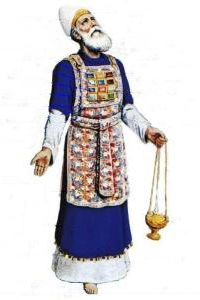
\includegraphics[width=50mm,scale=1.5]{Extras/Melchisedec.jpg}
\vspace{0.4in}  % Create a title for the document and write it in bold font
\LARGE{\textbf{\date}} % Again, do a line break
\linebreak 
% Create a subtitle \large{with Outlines, Statistics, Cross References, and Notes}
\vspace{0.5in}
\begin{flushleft}
\LARGE{Day \#72: Sunday, 13 March 2022  \\}\vspace{0.25in}
\LARGE{Joshua 22-24 Psalm 72 Proverb 13}
\end{flushleft}
\vspace{0.6in}
\bigskip

\normalsize{Xenia, Oh.\\}
\normalsize{created: \today}
\vspace{1.3in}

\end{flushright}
\end{titlepage}

\newpage 
\tableofcontents\hypertarget{TOC}{}
\listoffigures
\listoftables

\hyphenation{A-bim-e-lech bre-thren E-phra-im  Gib-e-o-nites Jer-u-sa-lem through-out Phil-i-stines The-o-phil-us Am-a-le-kites ven-geance Mesh-el-e-mi-ah onan-ism Phar-a-oh thoughts grev-ous-ness Hach-a-liah adul-ter-er Shad-rach}

%%%%%%%%%%%%%%%%% EXTRA COLORS
%%%%%%%%%%%%%%%%% EXTRA COLORS
%%%%%%%%%%%%%%%%% EXTRA COLORS
\definecolor{champagne}{rgb}{0.97,0.91,0.81}
\definecolor{bone}{rgb}{0.89,0.85,0.79}

\definecolor{ForestGreen}{rgb}{0.00,0.29,0.098}
\definecolor{GIVING}{cmyk}{1,0.0,0.72,.1}

\definecolor{MLPE}{cmyk}{1,1,0,.45}
\definecolor{SOCCER}{cmyk}{.77, 0, .42, .49}
\definecolor{PAYBILL}{cmyk}{0,0.83,0.76,0.07}
\definecolor{SERMON}{cmyk}{.14,.9,0,.30} % aka seance \href{http://www.flatuicolorpicker.com/purple-cmyk-color-model/}{seance}
\definecolor{BIBLE}{cmyk}{0,.17,.74,.17}
\definecolor{WORKBLUE}{cmyk}{1, .5, 0, .6}
\definecolor{myOrange}{cmyk}{0, .4, .98, .03}
\definecolor{myTan}{cmyk}{0.0,.07,.17,.10}
\definecolor{myRed}{cmyk}{0,1,1,0}
\definecolor{myWhite}{cmyk}{0,0,0,0}
\definecolor{BLUESoD}{cmyk}{.97,.84,0,.04}
\definecolor{WHITE}{cmyk}{0,0,0,0}
\definecolor{OLDGOLD}{cmyk}{0.05,0.3,1.00,0}
\definecolor{CASTLETON}{cmyk}{1,0,0.31,0.66}
\definecolor{cadmiumgreen}{rgb}{0.0, 0.42, 0.24}
\definecolor{jungle}{rgb}{0.203,0.4882,0.1718}
\definecolor{MYGOLD}{rgb}{1,.84,0}

\definecolor{MYLIGHTGRAY}{rgb}{.85,.85,.85}

\definecolor{codegreen}{rgb}{0,0.6,0}
\definecolor{codegray}{rgb}{0.5,0.5,0.5}
\definecolor{codepurple}{rgb}{0.58,0,0.82}
\definecolor{backcolour}{rgb}{0.95,0.95,0.92}


\mdfdefinestyle{MyFrame}{%
    linecolor=blue,
    outerlinewidth=2pt,
    roundcorner=5pt,
    innertopmargin=\baselineskip,
    innerbottommargin=\baselineskip,
    innerrightmargin=10pt,
    innerleftmargin=10pt,
    backgroundcolor=gray!25!white}


\mdfdefinestyle{MyFrame2}{%
    linecolor=black,
    outerlinewidth=2pt,
    roundcorner=5pt,
    innertopmargin=\baselineskip,
    innerbottommargin=\baselineskip,
    innerrightmargin=10pt,
    innerleftmargin=10pt,
    backgroundcolor=yellow!25!white}


%%%%%
%% for PFTTIS list
%%%%%

%%% And Joseph said unto
\index[PFTTIS]{And Joseph said unto!Genesis!Gen 40:008}
\index[PFTTIS]{And Joseph said unto!Genesis!Gen 40:012}
\index[PFTTIS]{And Joseph said unto!Genesis!Gen 41:025}
\index[PFTTIS]{And Joseph said unto!Genesis!Gen 42:014}
\index[PFTTIS]{And Joseph said unto!Genesis!Gen 42:018}
\index[PFTTIS]{And Joseph said unto!Genesis!Gen 44:015}
\index[PFTTIS]{And Joseph said unto!Genesis!Gen 45:003}
\index[PFTTIS]{And Joseph said unto!Genesis!Gen 45:004}
\index[PFTTIS]{And Joseph said unto!Genesis!Gen 46:031}
\index[PFTTIS]{And Joseph said unto!Genesis!Gen 48:009}
\index[PFTTIS]{And Joseph said unto!Genesis!Gen 48:018}
\index[PFTTIS]{And Joseph said unto!Genesis!Gen 50:019}
\index[PFTTIS]{And Joseph said unto!Genesis!Gen 50:024}


%%% a shadow
\index[PFTTIS]{a shadow!1Chronicles!1Chr 029:15}
\index[PFTTIS]{a shadow!Job!Job 008:09}
\index[PFTTIS]{a shadow!Job!Job 014:02}
\index[PFTTIS]{a shadow!Job!Job 017:07}
\index[PFTTIS]{a shadow!Psalm!Psa 102:011}
\index[PFTTIS]{a shadow!Psalm!Psa 144:004}
\index[PFTTIS]{a shadow!Ecclesiastes!Eccl 006:012}
\index[PFTTIS]{a shadow!Ecclesiastes!Eccl 008:013}
\index[PFTTIS]{a shadow!Isaiah!Isa 04:006}
\index[PFTTIS]{a shadow!Isaiah!Isa 25:004}
\index[PFTTIS]{a shadow!Jonah!Jnh 04:06}
\index[PFTTIS]{a shadow!Colossians!Col 02:017}
\index[PFTTIS]{a shadow!Hebews!Heb 10:001}

%%% blessed is the man
\index[PFTTIS]{blessed is the man!Psalm!Psa 001:001}
\index[PFTTIS]{blessed is the man!Psalm!Psa 032:002}
\index[PFTTIS]{blessed is the man!Psalm!Psa 034:008}
\index[PFTTIS]{blessed is the man!Psalm!Psa 065:004}
\index[PFTTIS]{blessed is the man!Psalm!Psa 084:005}
\index[PFTTIS]{blessed is the man!Psalm!Psa 084:012}
\index[PFTTIS]{blessed is the man!Psalm!Psa 094:012}
\index[PFTTIS]{blessed is the man!Psalm!Psa 112:001}
\index[PFTTIS]{blessed is the man!Proverbs!Pro 008:034}
\index[PFTTIS]{blessed is the man!Isaiah!Isa 056:002}
\index[PFTTIS]{blessed is the man!Jeremiah!Jer 017:007}
\index[PFTTIS]{blessed is the man!Romans!Rom 004:008}
\index[PFTTIS]{blessed is the man!James!Jam 001:012}


%%% carry them
\index[PFTTIS]{carry them!Leviticus!Lev 14:045}
\index[PFTTIS]{carry them!Numbers!Num 11:012}
\index[PFTTIS]{carry them!Joshua!Jsh 04:003}
\index[PFTTIS]{carry them!1Samuel!1Sam 20:040}
\index[PFTTIS]{carry them!1Kings!1Kng 08:046}
\index[PFTTIS]{carry them!2Chronicles!2Chr 06:036}
\index[PFTTIS]{carry them!Ezra!Ezra 05:015}
\index[PFTTIS]{carry them!Isaiah!Isa 40:011}
\index[PFTTIS]{carry them!Isaiah!Isa 41:016}
\index[PFTTIS]{carry them!Isaiah!Isa 57:013}
\index[PFTTIS]{carry them!Jeremiah!Jer 20:004}
\index[PFTTIS]{carry them!Jeremiah!Jer 20:005}
\index[PFTTIS]{carry them!Jeremiah!Jer 43:012}


\index[PFTTIS]{good tidings!2Samuel!2Sam 18:027}
\index[PFTTIS]{good tidings!1Kings!1Ki 01:042}
\index[PFTTIS]{good tidings!2Kings!2Ki 07:009 (2x)}
\index[PFTTIS]{good tidings!Isaiah!Isa 40:009 (2x)}
\index[PFTTIS]{good tidings!Isaiah!Isa 41:007}
\index[PFTTIS]{good tidings!Isaiah!Isa 52:007}
\index[PFTTIS]{good tidings!Isaiah!Isa 61:001}
\index[PFTTIS]{good tidings!Nahum!Nah 01:005}
\index[PFTTIS]{good tidings!Luke!Lk 02:010}
\index[PFTTIS]{good tidings!1Thessalonians!1Thess 03:006}


%%% dead body
\index[PFTTIS]{dead body!Leviticus!Lev 21:011}
\index[PFTTIS]{dead body!Numbers!Num 06:006}
\index[PFTTIS]{dead body!Numbers!Num 09:006}
\index[PFTTIS]{dead body!Numbers!Num 09:007}
\index[PFTTIS]{dead body!Numbers!Num 09:010}
\index[PFTTIS]{dead body!Numbers!Num 09:011}
\index[PFTTIS]{dead body!Numbers!Num 09:013}
\index[PFTTIS]{dead body!Numbers!Num 09:016}
\index[PFTTIS]{dead body!2Kings!2Ki 08:005}
\index[PFTTIS]{dead body!Isaiah!Isa 26:019}
\index[PFTTIS]{dead body!Jeremiah!Jer 26:023}
\index[PFTTIS]{dead body!Jeremiah!Jer 36:030}
\index[PFTTIS]{dead body!Haggai!Hag 02:013}

%%% great sea
\index[PFTTIS]{great sea!Numbers!Num 34:006}
\index[PFTTIS]{great sea!Numbers!Num 34:007}
\index[PFTTIS]{great sea!Joshua!Jos 01:004}
\index[PFTTIS]{great sea!Joshua!Jos 09:001}
\index[PFTTIS]{great sea!Joshua!Jos 15:012}
\index[PFTTIS]{great sea!Joshua!Jos 15:047}
\index[PFTTIS]{great sea!Joshua!Jos 23:004}
\index[PFTTIS]{great sea!Ezekiel!Eze 47:010}
\index[PFTTIS]{great sea!Ezekiel!Eze 47:015}
\index[PFTTIS]{great sea!Ezekiel!Eze 47:019}
\index[PFTTIS]{great sea!Ezekiel!Eze 47:020}
\index[PFTTIS]{great sea!Ezekiel!Eze 48:028}
\index[PFTTIS]{great sea!Daniel!Dan 07:002}


%%% have forsaken me
\index[PFTTIS]{have forsaken me!Judges!Jdg 10:013}
\index[PFTTIS]{have forsaken me!1Samuel!1Sam 08:008}
\index[PFTTIS]{have forsaken me!1Kings!1Ki 11:033}
\index[PFTTIS]{have forsaken me!2Kings!2Ki 22:017}
\index[PFTTIS]{have forsaken me!2Chronicles!2Chr 12:005}
\index[PFTTIS]{have forsaken me!2Chronicles!2Chr 34:025}
\index[PFTTIS]{have forsaken me!Jeremiah!Jer 01:016}
\index[PFTTIS]{have forsaken me!Jeremiah!Jer 02:013}
\index[PFTTIS]{have forsaken me!Jeremiah!Jer 05:007}
\index[PFTTIS]{have forsaken me!Jeremiah!Jer 05:019}
\index[PFTTIS]{have forsaken me!Jeremiah!Jer 16:011 (2x)}
\index[PFTTIS]{have forsaken me!Jeremiah!Jer 19:004}

%%% no king
\index[PFTTIS]{no king!Judges!Jdg 17:06}
\index[PFTTIS]{no king!Judges!Jdg 18:01}
\index[PFTTIS]{no king!Judges!Jdg 19:01}
\index[PFTTIS]{no king!Judges!Jdg 21:25}
\index[PFTTIS]{no king!1Kings!1Ki 22:47}
\index[PFTTIS]{no king!2Kings!2Ki 23:25}
\index[PFTTIS]{no king!Nehemiah!Neh 13:26}
\index[PFTTIS]{no king!Psalms!Psa 033:016}
\index[PFTTIS]{no king!Proverbs!Pro 30:27}
\index[PFTTIS]{no king!Daniel!Dan 02:10}
\index[PFTTIS]{no king!Hosea!Hos 10:03}
\index[PFTTIS]{no king!Micah!Mic 04:09}
\index[PFTTIS]{no king!John!Jhn 19:15}


%%% rebellious house
\index[PFTTIS]{rebellious house!Exodus!Exo 02:005}
\index[PFTTIS]{rebellious house!Exodus!Exo 02:006}
\index[PFTTIS]{rebellious house!Exodus!Exo 02:008}
\index[PFTTIS]{rebellious house!Exodus!Exo 03:009}
\index[PFTTIS]{rebellious house!Exodus!Exo 03:026}
\index[PFTTIS]{rebellious house!Exodus!Exo 03:027}
\index[PFTTIS]{rebellious house!Exodus!Exo 12:002 (2x)}
\index[PFTTIS]{rebellious house!Exodus!Exo 12:003}
\index[PFTTIS]{rebellious house!Exodus!Exo 12:009}
\index[PFTTIS]{rebellious house!Exodus!Exo 12:025}
\index[PFTTIS]{rebellious house!Exodus!Exo 17:012}
\index[PFTTIS]{rebellious house!Exodus!Exo 24:003}

%%% seek him
\index[PFTTIS]{seek him!Deuteronomy!Deu 04:029}\index[PFTTIS]{seek him!1Samuel!1Sam 23:025}
\index[PFTTIS]{seek him!1Chronicles!1Chr 28:009}
\index[PFTTIS]{seek him!2Chronicles!1Chr 15:002}
\index[PFTTIS]{seek him!Ezra!Ezr 08:022}
\index[PFTTIS]{seek him!Psalms!Psa 022:026}
\index[PFTTIS]{seek him!Psalms!Psa 024:006}
\index[PFTTIS]{seek him!Psalms!Psa 119:002}
\index[PFTTIS]{seek him!SoS!SoS 03:002}
\index[PFTTIS]{seek him!SoS!SoS 06:001}
\index[PFTTIS]{seek him!Hosea!Hos 07:010}
\index[PFTTIS]{seek him!Amos!Amo 05:008}
\index[PFTTIS]{seek him!Hebrews!Heb 11:0063}


%%% seek ye
\index[PFTTIS]{seek ye!Isaiah!Isa 34:016}
\index[PFTTIS]{seek ye!Isaiah!Isa 45:019}
\index[PFTTIS]{seek ye!Isaiah!Isa 55:006}
\index[PFTTIS]{seek ye!Amos!Amos 5:004}
\index[PFTTIS]{seek ye!John!John 1:38}
\index[PFTTIS]{seek ye!John!John 18:4}
\index[PFTTIS]{seek ye!John!John 18:7}
\index[PFTTIS]{seek ye!Matthew!Matt 6:33}
\index[PFTTIS]{seek ye!Numbers!Num 16:10}
\index[PFTTIS]{seek ye!Luke!Luke 12:31}
\index[PFTTIS]{seek ye!Luke!Luke 24:5}
\index[PFTTIS]{seek ye!Psalm!Psa 27:8}
\index[PFTTIS]{seek ye!Zephaniah!Zeph 2:3}

%%% the uncircumcised
\index[PFTTIS]{the uncircumcised!Genesis!Gen 17:014}
\index[PFTTIS]{the uncircumcised!Judges!Jdg 14:003}
\index[PFTTIS]{the uncircumcised!Judges!Jdg 15:018}
\index[PFTTIS]{the uncircumcised!2Samuel!2Sam 01:020}
\index[PFTTIS]{the uncircumcised!Isaiah!Isa 02:001}
\index[PFTTIS]{the uncircumcised!Jeremiah!Jer 09:025}
\index[PFTTIS]{the uncircumcised!Ezekiel!Eze 28:010}
\index[PFTTIS]{the uncircumcised!Ezekiel!Eze 31:018}
\index[PFTTIS]{the uncircumcised!Ezekiel!Eze 32:019}
\index[PFTTIS]{the uncircumcised!Ezekiel!Eze 32:027}
\index[PFTTIS]{the uncircumcised!Ezekiel!Eze 32:028}
\index[PFTTIS]{the uncircumcised!Ezekiel!Eze 32:029}
\index[PFTTIS]{the uncircumcised!Ezekiel!Eze 32:032}

%%% worship him
\index[PFTTIS]{worship him!Psalms!Psa 97:007}
\index[PFTTIS]{worship him!Zephaniah!Zeph 02:011}
\index[PFTTIS]{worship him!Matthew!Matt 02:002}
\index[PFTTIS]{worship him!Matthew!Matt 02:008}
\index[PFTTIS]{worship him!John!John 04:023}
\index[PFTTIS]{worship him!John!John 04:024 (2x)} 
\index[PFTTIS]{worship him!Acts!Acts 17:023}
\index[PFTTIS]{worship him!Hebrews!Heb 01:006}
\index[PFTTIS]{worship him!Revelation!Rev 04:010}
\index[PFTTIS]{worship him!Revelation!Rev 13:008}
\index[PFTTIS]{worship him!Revelation!Rev 14:007}
\index[PFTTIS]{worship him!Revelation!Rev 19:010}


%%%%%
%% for PFTTIS list
%%%%%

%%% afflictions
\index[WFTTIS]{afflictions!Psalms!Psa 34:019}
\index[WFTTIS]{afflictions!Psalms!Psa 132:001}
\index[WFTTIS]{afflictions!Acts!Acts 07:010}
\index[WFTTIS]{afflictions!Acts!Acts 20:023}
\index[WFTTIS]{afflictions!2Corinthians!2Cor 06:004}
\index[WFTTIS]{afflictions!Colossians!Col 01:024}
\index[WFTTIS]{afflictions!1Thessalonians!1Thess 03:003}
\index[WFTTIS]{afflictions!2Timothy!2Tim 01:008}
\index[WFTTIS]{afflictions!2Timothy!2Tim 03:011}
\index[WFTTIS]{afflictions!2Timothy!2Tim 04:005}
\index[WFTTIS]{afflictions!Hebrews!Heb 10:032}
\index[WFTTIS]{afflictions!Hebrews!Heb 10:033}
\index[WFTTIS]{afflictions!1Peter!1Pet 05:009}

%%% acsend
\index[WFTTIS]{acsend!Joshua!Jos 06:05}
\index[WFTTIS]{acsend!Psalm!Psa 024:003}
\index[WFTTIS]{acsend!Psalm!Psa 135:007}
\index[WFTTIS]{acsend!Psalm!Psa 139:008}
\index[WFTTIS]{acsend!Isaiah!Isa 14:013}
\index[WFTTIS]{acsend!Isaiah!Isa 14:014}
\index[WFTTIS]{acsend!Jeremiah!Jer 10:013}
\index[WFTTIS]{acsend!Jeremiah!Jer 51:016}
\index[WFTTIS]{acsend!Ezekiel!Eze 38:009}
\index[WFTTIS]{acsend!John!John 06:062}
\index[WFTTIS]{acsend!John!John 20:017}
\index[WFTTIS]{acsend!Romans!Rom 10:006}
\index[WFTTIS]{acsend!Revelation!Rev 17:008}

%%% Assyrian
\index[WFTTIS]{Assyrian!Isaiah!Isa 10:005}
\index[WFTTIS]{Assyrian!Isaiah!Isa 10:024}
\index[WFTTIS]{Assyrian!Isaiah!Isa 14:025}
\index[WFTTIS]{Assyrian!Isaiah!Isa 19:023}
\index[WFTTIS]{Assyrian!Isaiah!Isa 23:013}
\index[WFTTIS]{Assyrian!Isaiah!Isa 30:031}
\index[WFTTIS]{Assyrian!Isaiah!Isa 31:008}
\index[WFTTIS]{Assyrian!Isaiah!Isa 52:004}
\index[WFTTIS]{Assyrian!Ezekiel!Eze 31:003}
\index[WFTTIS]{Assyrian!Hosea!Hos 05:013}
\index[WFTTIS]{Assyrian!Hosea!Hos 11:005}
\index[WFTTIS]{Assyrian!Micah!Hos 05:005}
\index[WFTTIS]{Assyrian!Micah!Hos 05:006}

%%% blot
\index[WFTTIS]{blot!Exodus!Exo 32:032}
\index[WFTTIS]{blot!Exodus!Exo 32:033}
\index[WFTTIS]{blot!Numbers!Num 05:026}
\index[WFTTIS]{blot!Deuteronomy!Deut 09:014}
\index[WFTTIS]{blot!Deuteronomy!Deut 25:019}
\index[WFTTIS]{blot!Deuteronomy!Deut 29:020}
\index[WFTTIS]{blot!2Kings!2Ki 14:027}
\index[WFTTIS]{blot!Job!Job 31:007}
\index[WFTTIS]{blot!Psalms!Psa 51:001}
\index[WFTTIS]{blot!Psalms!Psa 51:009}
\index[WFTTIS]{blot!Proverbs!Pro 09:007}
\index[WFTTIS]{blot!Jeremiah!Jer 18:023}
\index[WFTTIS]{blot!Revelation!Rev 03:005}


%%% chain
\index[WFTTIS]{chain!Genesis!Gen 41:042}
\index[WFTTIS]{chain!1Kings!1Ki 07:017}
\index[WFTTIS]{chain!Psalms!Psa 73:006}
\index[WFTTIS]{chain!SoS!Sos 04:009}
\index[WFTTIS]{chain!Lamentations!Lam 03:007}
\index[WFTTIS]{chain!Ezekiel!Eze 07:023}
\index[WFTTIS]{chain!Ezekiel!Eze 16:011}
\index[WFTTIS]{chain!Daniel!Dan 05:007}
\index[WFTTIS]{chain!Daniel!Dan 05:016}
\index[WFTTIS]{chain!Daniel!Dan 05:029}
\index[WFTTIS]{chain!Acts!Acts 28:020}
\index[WFTTIS]{chain!2Timothy!2Tim 01:016}
\index[WFTTIS]{chain!Revelation!Rev 20:001}


%%% controversy
\index[WFTTIS]{controversy!Deuteronomy!Deu 17:008}
\index[WFTTIS]{controversy!Deuteronomy!Deu 19:017}
\index[WFTTIS]{controversy!Deuteronomy!Deu 21:005}
\index[WFTTIS]{controversy!Deuteronomy!Deu 25:001}
\index[WFTTIS]{controversy!2Samuel!2Sam 15:002}
\index[WFTTIS]{controversy!Isaiah!Isa 34:008}
\index[WFTTIS]{controversy!Jeremiah!Jer 25:031}
\index[WFTTIS]{controversy!Ezekiel!Eze 44:024}
\index[WFTTIS]{controversy!Hosea!Hos 04:001}
\index[WFTTIS]{controversy!Hosea!Hos 12:002}
\index[WFTTIS]{controversy!Micah!Mic 06:002 (2x)}
\index[WFTTIS]{controversy!1Timothy!1Tim 03:016}


%%% Dagon/Dagon's
\index[WFTTIS]{Dagon!Judges!Jdg 16:023}
\index[WFTTIS]{Dagon!1Samuel!1Sam 05:002 (2x)}
\index[WFTTIS]{Dagon!1Samuel!1Sam 05:003 (2x)}
\index[WFTTIS]{Dagon!1Samuel!1Sam 05:004 (3x)}
\index[WFTTIS]{Dagon!1Samuel!1Sam 05:005 (3x)}
\index[WFTTIS]{Dagon!1Samuel!1Sam 05:007}
\index[WFTTIS]{Dagon!1Chronicles!1Chr 10:010}

%%% disobedient
\index[WFTTIS]{disobedient!1Kings!1Ki 13:026}
\index[WFTTIS]{disobedient!Nehemiah!Neh 09:026}
\index[WFTTIS]{disobedient!Luke!Luke 01:017}
\index[WFTTIS]{disobedient!Acts!Acts 26:019}
\index[WFTTIS]{disobedient!Romans!Rom 01:030}
\index[WFTTIS]{disobedient!Romans!Rom 10:021}
\index[WFTTIS]{disobedient!1Timothy!1Tim 01:009}
\index[WFTTIS]{disobedient!2Timothy!2Tim 03:002}
\index[WFTTIS]{disobedient!Titus!Titus 01:016}
\index[WFTTIS]{disobedient!Titus!Titus 03:003}
\index[WFTTIS]{disobedient!1Peter!1Pet 02:007}
\index[WFTTIS]{disobedient!1Peter!1Pet 02:008}
\index[WFTTIS]{disobedient!1Peter!1Pet 03:020}


%%% doubt
\index[WFTTIS]{doubt!Genesis!Gen 37:033}
\index[WFTTIS]{doubt!Deuteronomy!Deu 28:066}
\index[WFTTIS]{doubt!Job!Job 12:002}
\index[WFTTIS]{doubt!Matthew!Matt 14:031}
\index[WFTTIS]{doubt!Matthew!Matt 21:021}
\index[WFTTIS]{doubt!Mark!Mk 11:023}
\index[WFTTIS]{doubt!Luke!Lk 11:020}
\index[WFTTIS]{doubt!John!Jhn 10:024}
\index[WFTTIS]{doubt!Acts!Acts 02:012}
\index[WFTTIS]{doubt!Acts!Acts 28:004}
\index[WFTTIS]{doubt!1Corinthians!1Cor 09:010}
\index[WFTTIS]{doubt!Galatians!Gal 04:020}
\index[WFTTIS]{doubt!1John!1Jhn 02:019}


%%% dungeon
\index[WFTTIS]{dungeon!Genesis!Gen 40:015}
\index[WFTTIS]{dungeon!Genesis!Gen 41:014}
\index[WFTTIS]{dungeon!Exodus!Exo 12:029}
\index[WFTTIS]{dungeon!Jeremiah!Jer 37:016}
\index[WFTTIS]{dungeon!Jeremiah!Jer 38:006 (2x)}
\index[WFTTIS]{dungeon!Jeremiah!Jer 38:007}
\index[WFTTIS]{dungeon!Jeremiah!Jer 38:009}
\index[WFTTIS]{dungeon!Jeremiah!Jer 38:010}
\index[WFTTIS]{dungeon!Jeremiah!Jer 38:011}
\index[WFTTIS]{dungeon!Jeremiah!Jer 38:013}
\index[WFTTIS]{dungeon!Lamentations!Lam 03:053}
\index[WFTTIS]{dungeon!Lamentations!Lam 03:055}


%%% error
\index[WFTTIS]{error!2Samuel!2Sam 06:007}
\index[WFTTIS]{error!Job!Job 19:004}
\index[WFTTIS]{error!Ecclesiastes!Ecc 05:006}
\index[WFTTIS]{error!Ecclesiastes!Ecc 10:005}
\index[WFTTIS]{error!Isaiah!Isa 32:006}
\index[WFTTIS]{error!Daniel!Dan 06:004}
\index[WFTTIS]{error!Matthew!Matt 27:064}
\index[WFTTIS]{error!Romans!Rom 01:027}
\index[WFTTIS]{error!James!Jam 05:020}
\index[WFTTIS]{error!2Peter!2Pet 02:018}
\index[WFTTIS]{error!2Peter!2Pet 03:017}
\index[WFTTIS]{error!1John!1Jn 04:006}
\index[WFTTIS]{error!Jude!Jude 01:011}

%%% fourish
\index[WFTTIS]{fourish!Psalms!Psa 072:007}
\index[WFTTIS]{fourish!Psalms!Psa 072:016}
\index[WFTTIS]{fourish!Psalms!Psa 092:007}
\index[WFTTIS]{fourish!Psalms!Psa 092:012}
\index[WFTTIS]{fourish!Psalms!Psa 092:013}
\index[WFTTIS]{fourish!Psalms!Psa 132:018}
\index[WFTTIS]{fourish!Proverbs!Pro 11:28}
\index[WFTTIS]{fourish!Proverbs!Pro 14:11}
\index[WFTTIS]{fourish!Ecclesiastes!Ecc 12:05}
\index[WFTTIS]{fourish!SongOfSolomon!SOS 07:12}
\index[WFTTIS]{fourish!Isaiah!Isa 17:11}
\index[WFTTIS]{fourish!Isaiah!Isa 66:14}
\index[WFTTIS]{fourish!Ezekiel!Eze 17:24}




%%% giants
\index[WFTTIS]{giants!Genesis!Gen 06:004}
\index[WFTTIS]{giants!Numbers!Num 13:033}
\index[WFTTIS]{giants!Deuteronomy!Deut 02:011}
\index[WFTTIS]{giants!Deuteronomy!Deut 02:021}
\index[WFTTIS]{giants!Deuteronomy!Deut 03:011}
\index[WFTTIS]{giants!Deuteronomy!Deut 03:013}
\index[WFTTIS]{giants!Joshua!Josh 12:004}
\index[WFTTIS]{giants!Joshua!Josh 13:012}
\index[WFTTIS]{giants!Joshua!Josh 15:008}
\index[WFTTIS]{giants!Joshua!Josh 17:015}
\index[WFTTIS]{giants!Joshua!Josh 16:016}

%%% good man
\index[WFTTIS]{good man!2 Samuel!2Sa 18:27}
%(1) Psalms 37:23 [5]
%(1) Psalms 112:5 [2]
%(1) Proverbs 12:2 [2]
%(1) Proverbs 13:22 [2]
%(1) Proverbs 14:14 [14]
%(1) Micah 7:2 [2]
%(1) Matthew 12:35 [2]
%(1) Luke 6:45 [2]
%(1) Luke 23:50 [15]
%(1) John 7:12 [17]
%(1) Acts 11:24 [5]
%(1) Romans 5:7 [14]

%%% Hinnom
\index[WFTTIS]{Hinnom!Joshua!Jsh 15:008}
\index[WFTTIS]{Hinnom!Joshua!Jsh 18:016}
\index[WFTTIS]{Hinnom!2Kings!2Ki 23:010}
\index[WFTTIS]{Hinnom!2Chronicles!2Chr 28:003}
\index[WFTTIS]{Hinnom!2Chronicles!2Chr 33:006}
\index[WFTTIS]{Hinnom!Nehemiah!Neh 11:030}
\index[WFTTIS]{Hinnom!Jeremiah!Jer 07:031}
\index[WFTTIS]{Hinnom!Jeremiah!Jer 07:032}
\index[WFTTIS]{Hinnom!Jeremiah!Jer 19:002}
\index[WFTTIS]{Hinnom!Jeremiah!Jer 19:006}
\index[WFTTIS]{Hinnom!Jeremiah!Jer 32:035}

%%% inclined
\index[WFTTIS]{inclined!Judges!Jdg 09:003}
\index[WFTTIS]{inclined!Psalms!Psa 040:001}
\index[WFTTIS]{inclined!Psalms!Psa 116:002}
\index[WFTTIS]{inclined!Psalms!Psa 119:112}
\index[WFTTIS]{inclined!Proverbs!Pro 05:13}
\index[WFTTIS]{inclined!Jeremiah!Jer 07:24}
\index[WFTTIS]{inclined!Jeremiah!Jer 07:26}
\index[WFTTIS]{inclined!Jeremiah!Jer 11:08}
\index[WFTTIS]{inclined!Jeremiah!Jer 17:23}
\index[WFTTIS]{inclined!Jeremiah!Jer 25:04}
\index[WFTTIS]{inclined!Jeremiah!Jer 34:14}
\index[WFTTIS]{inclined!Jeremiah!Jer 35:15}
\index[WFTTIS]{inclined!Jeremiah!Jer 44:05}


%%% laughed
\index[WFTTIS]{laughed!Genesis!Gen 17:017}
\index[WFTTIS]{laughed!Genesis!Gen 18:012}
\index[WFTTIS]{laughed!Genesis!Gen 18:015}
\index[WFTTIS]{laughed!2Kings!2Ki 19:021}
\index[WFTTIS]{laughed!2Chronicles!2Chr 30:010}
\index[WFTTIS]{laughed!Nehemiah!Neh 02:019}
\index[WFTTIS]{laughed!Job!Job 12:004}
\index[WFTTIS]{laughed!Job!Job 29:024}
\index[WFTTIS]{laughed!Isaiah!Isa 37:022}
\index[WFTTIS]{laughed!Ezekiel!Ezek 23:032}
\index[WFTTIS]{laughed!Matthew!Matt 09:024}
\index[WFTTIS]{laughed!Mark!Mk 05:040}
\index[WFTTIS]{laughed!Luke!Lk 08:053}

%%% liar
\index[WFTTIS]{liar!Job!Job 24:025}
\index[WFTTIS]{liar!Proverbs!Pro 17:004}
\index[WFTTIS]{liar!Proverbs!Pro 19:022}
\index[WFTTIS]{liar!Proverbs!Pro 30:006}
\index[WFTTIS]{liar!Jeremiah!Jer 15:018}
\index[WFTTIS]{liar!John!Jhn 08:044}
\index[WFTTIS]{liar!John!Jhn 08:055}
\index[WFTTIS]{liar!Romans!Rom 03:004}
\index[WFTTIS]{liar!1John!1Jhn 01:010}
\index[WFTTIS]{liar!1John!1Jhn 02:004}
\index[WFTTIS]{liar!1John!1Jhn 02:022}
\index[WFTTIS]{liar!1John!1Jhn 04:020}
\index[WFTTIS]{liar!1John!1Jhn 05:010}

%%% palsy
\index[WFTTIS]{palsy!Matthew!Matt 04:024}
\index[WFTTIS]{palsy!Matthew!Matt 08:006}
\index[WFTTIS]{palsy!Matthew!Matt 09:002}
\index[WFTTIS]{palsy!Matthew!Matt 09:006}
\index[WFTTIS]{palsy!Mark!Mk 02:003}
\index[WFTTIS]{palsy!Mark!Mk 02:004}
\index[WFTTIS]{palsy!Mark!Mk 02:005}
\index[WFTTIS]{palsy!Mark!Mk 02:009}
\index[WFTTIS]{palsy!Mark!Mk 02:010}
\index[WFTTIS]{palsy!Luke!Lk 05:018}
\index[WFTTIS]{palsy!Luke!Lk 05:024}
\index[WFTTIS]{palsy!Acts!Acts 09:033}

%%% Profitable
\index[WFTTIS]{profitable!Job!Job 22:002 (2x)}
\index[WFTTIS]{profitable!Ecclesiastes!Ecc 10:010}
\index[WFTTIS]{profitable!Isaiah!Isa 44:010}
\index[WFTTIS]{profitable!Jeremiah!Jer 13:007}
\index[WFTTIS]{profitable!Matthew!Matt 05:029}
\index[WFTTIS]{profitable!Matthew!Matt 05:030}
\index[WFTTIS]{profitable!Acts!Acts 20:020}
\index[WFTTIS]{profitable!1Timothy!1Tim 04:008}
\index[WFTTIS]{profitable!2Timothy!2Tim 03:016}
\index[WFTTIS]{profitable!2Timothy!2Tim 04:011}
\index[WFTTIS]{profitable!Titus!Titus 03:008}
\index[WFTTIS]{profitable!Philemon!Phlm 01:011}

%%% Rechab
\index[WFTTIS]{Rechab!2Samuel!2Sam 04:002}
\index[WFTTIS]{Rechab!2Samuel!2Sam 04:005}
\index[WFTTIS]{Rechab!2Samuel!2Sam 04:006}
\index[WFTTIS]{Rechab!2Samuel!2Sam 04:009}
\index[WFTTIS]{Rechab!2KIngs!2Ki 10:015}
\index[WFTTIS]{Rechab!2KIngs!2Ki 10:023}
\index[WFTTIS]{Rechab!1Chronicles!1Chr 02:055}
\index[WFTTIS]{Rechab!Nehemiah!Neh 03:014}
\index[WFTTIS]{Rechab!Jeremiah!Jer 35:006}
\index[WFTTIS]{Rechab!Jeremiah!Jer 35:008}
\index[WFTTIS]{Rechab!Jeremiah!Jer 35:014}
\index[WFTTIS]{Rechab!Jeremiah!Jer 35:016}
\index[WFTTIS]{Rechab!Jeremiah!Jer 35:019}

%%% serpents
\index[WFTTIS]{serpents!Exodus!Exo 07:012}
\index[WFTTIS]{serpents!Numbers!Num 21:006}
\index[WFTTIS]{serpents!Numbers!Num 21:007}
\index[WFTTIS]{serpents!Deuteronomy!Deu 08:015}
\index[WFTTIS]{serpents!Deuteronomy!Deu 32:024}
\index[WFTTIS]{serpents!Jeremiah!Jer 08:017}
\index[WFTTIS]{serpents!Matthew!Matt 10:016}
\index[WFTTIS]{serpents!Matthew!Matt 23:033}
\index[WFTTIS]{serpents!Mark!Mk 16:018}
\index[WFTTIS]{serpents!Luke!Lk 10:019}
\index[WFTTIS]{serpents!1Corinthians!1Cor 10:009}
\index[WFTTIS]{serpents!James!Jas 03:007}
\index[WFTTIS]{serpents!Revelation!Rev 09:019}

%%% short
\index[WFTTIS]{short!Numbers!Num 11:023}
\index[WFTTIS]{short!2Kings!2Ki 10:032}
\index[WFTTIS]{short!Job!Job 17:012}
\index[WFTTIS]{short!Job!Job 20:005}
\index[WFTTIS]{short!Psalms!Psa 89:047}
\index[WFTTIS]{short!Romans!Rom 03:023}
\index[WFTTIS]{short!Romans!Rom 09:028  (2x)}
\index[WFTTIS]{short!1Corinthians!1Cor 07:029}
\index[WFTTIS]{short!1Thessalonians!1Thess 02:017}
\index[WFTTIS]{short!Hebrews!Heb 04:001}
\index[WFTTIS]{short!Revelation!Rev 12:012}
\index[WFTTIS]{short!Revelation!Rev 17:010}

%%% smiteth
\index[WFTTIS]{smiteth!Exodus!Exo 21:012}
\index[WFTTIS]{smiteth!Exodus!Exo 21:15}
\index[WFTTIS]{smiteth!Deuteronomy!Dt 25:11}
\index[WFTTIS]{smiteth!Deuteronomy!Dt 27:24}
\index[WFTTIS]{smiteth!Joshua!Jsh 15:16}
\index[WFTTIS]{smiteth!Judges!Jdg 15:16}
\index[WFTTIS]{smiteth!2 Samuel!2Sa 05:08}
\index[WFTTIS]{smiteth!1Chronicles!1Chr 11:06}
\index[WFTTIS]{smiteth!Job!1Chr 26:12}
\index[WFTTIS]{smiteth!Isaiah!Isa 09:13}
\index[WFTTIS]{smiteth!Lamentations!Lam 03:30}
\index[WFTTIS]{smiteth!Ezekiel!Eze 07:09}
\index[WFTTIS]{smiteth!Luke!Lk 06:29}



%%% vanities
\index[WFTTIS]{vanities!Deuteronomy!Deut 21:021}
\index[WFTTIS]{vanities!1Kings!1Ki 16:013}
\index[WFTTIS]{vanities!1Kings!1Ki 16:026}
\index[WFTTIS]{vanities!Psalms!Psa 031:006}
\index[WFTTIS]{vanities!Ecclesiastes!Ecc 01:002 (2x)}
\index[WFTTIS]{vanities!Ecclesiastes!Ecc 05:007}
\index[WFTTIS]{vanities!Ecclesiastes!Ecc 12:008}
\index[WFTTIS]{vanities!Jeremiah!Jer 08:019}
\index[WFTTIS]{vanities!Jeremiah!Jer 10:008}
\index[WFTTIS]{vanities!Jeremiah!Jer 14:022}
\index[WFTTIS]{vanities!Jonah!Jnh 02:008}
\index[WFTTIS]{vanities!Acts!Acts 14:015}



%%%%%
%% for PFTTIS list
%%%%%

%%% worm
\index[WFITV]{worm!Exodus!Exo 16:024}
\index[WFITV]{worm!Job!Job 17:014}
\index[WFITV]{worm!Job!Job 24:029}
\index[WFITV]{worm!Job!Job 25:005 (2x)}
\index[WFITV]{worm!Psalms!Psa 022:006}
\index[WFITV]{worm!Isaiah!Isa 14:011}
\index[WFITV]{worm!Isaiah!Isa 41:014}
\index[WFITV]{worm!Isaiah!Isa 51:008}
\index[WFITV]{worm!Isaiah!Isa 66:024}
\index[WFITV]{worm!Jonah!Jnh 04:007}
\index[WFITV]{worm!Mark!Mk 09:044}
\index[WFITV]{worm!Mark!Mk 09:046}
\index[WFITV]{worm!Mark!Mk 09:048}


%\subsubsection{Title}
%\textbf{Introduction:} Isaiah 46 
%\index[speaker]{Speaker!Isaiah 49 (Title}
%\index[series]{Book (Speaker)!IPassage (Title)}
%\index[date]{2017/07/09!Isaiah 49 (Title)}
%\begin{compactenum}[I.]
%    \item  \textbf{Point} \index[scripture]{Isaiah!IPassage} (IPassage)
%\end{compactenum}




  


%\input{02OT-Exodus/ExodusIntroduction}

%\newpage
%\begin{figure}
%\begin{center}
%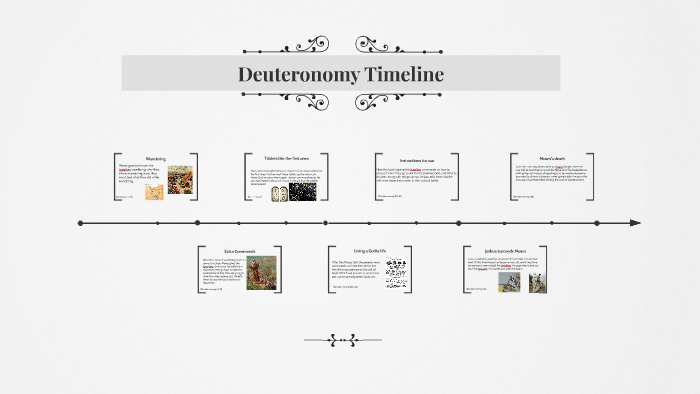
\includegraphics[scale=.7, angle=0]{05OT-Deuteronomy/References/AndrewSmithDeuteronomyTimeline.png}
%\caption[Deuteronomy Timeline by Andrew Smith]{Deuteronomy Timeline by Andrew %Smith}
%\label{fig:Deuteronomy Timeline by Andrew Smith}
%\end{center}
%\end{figure}

\newpage
\begin{figure}
\begin{center}
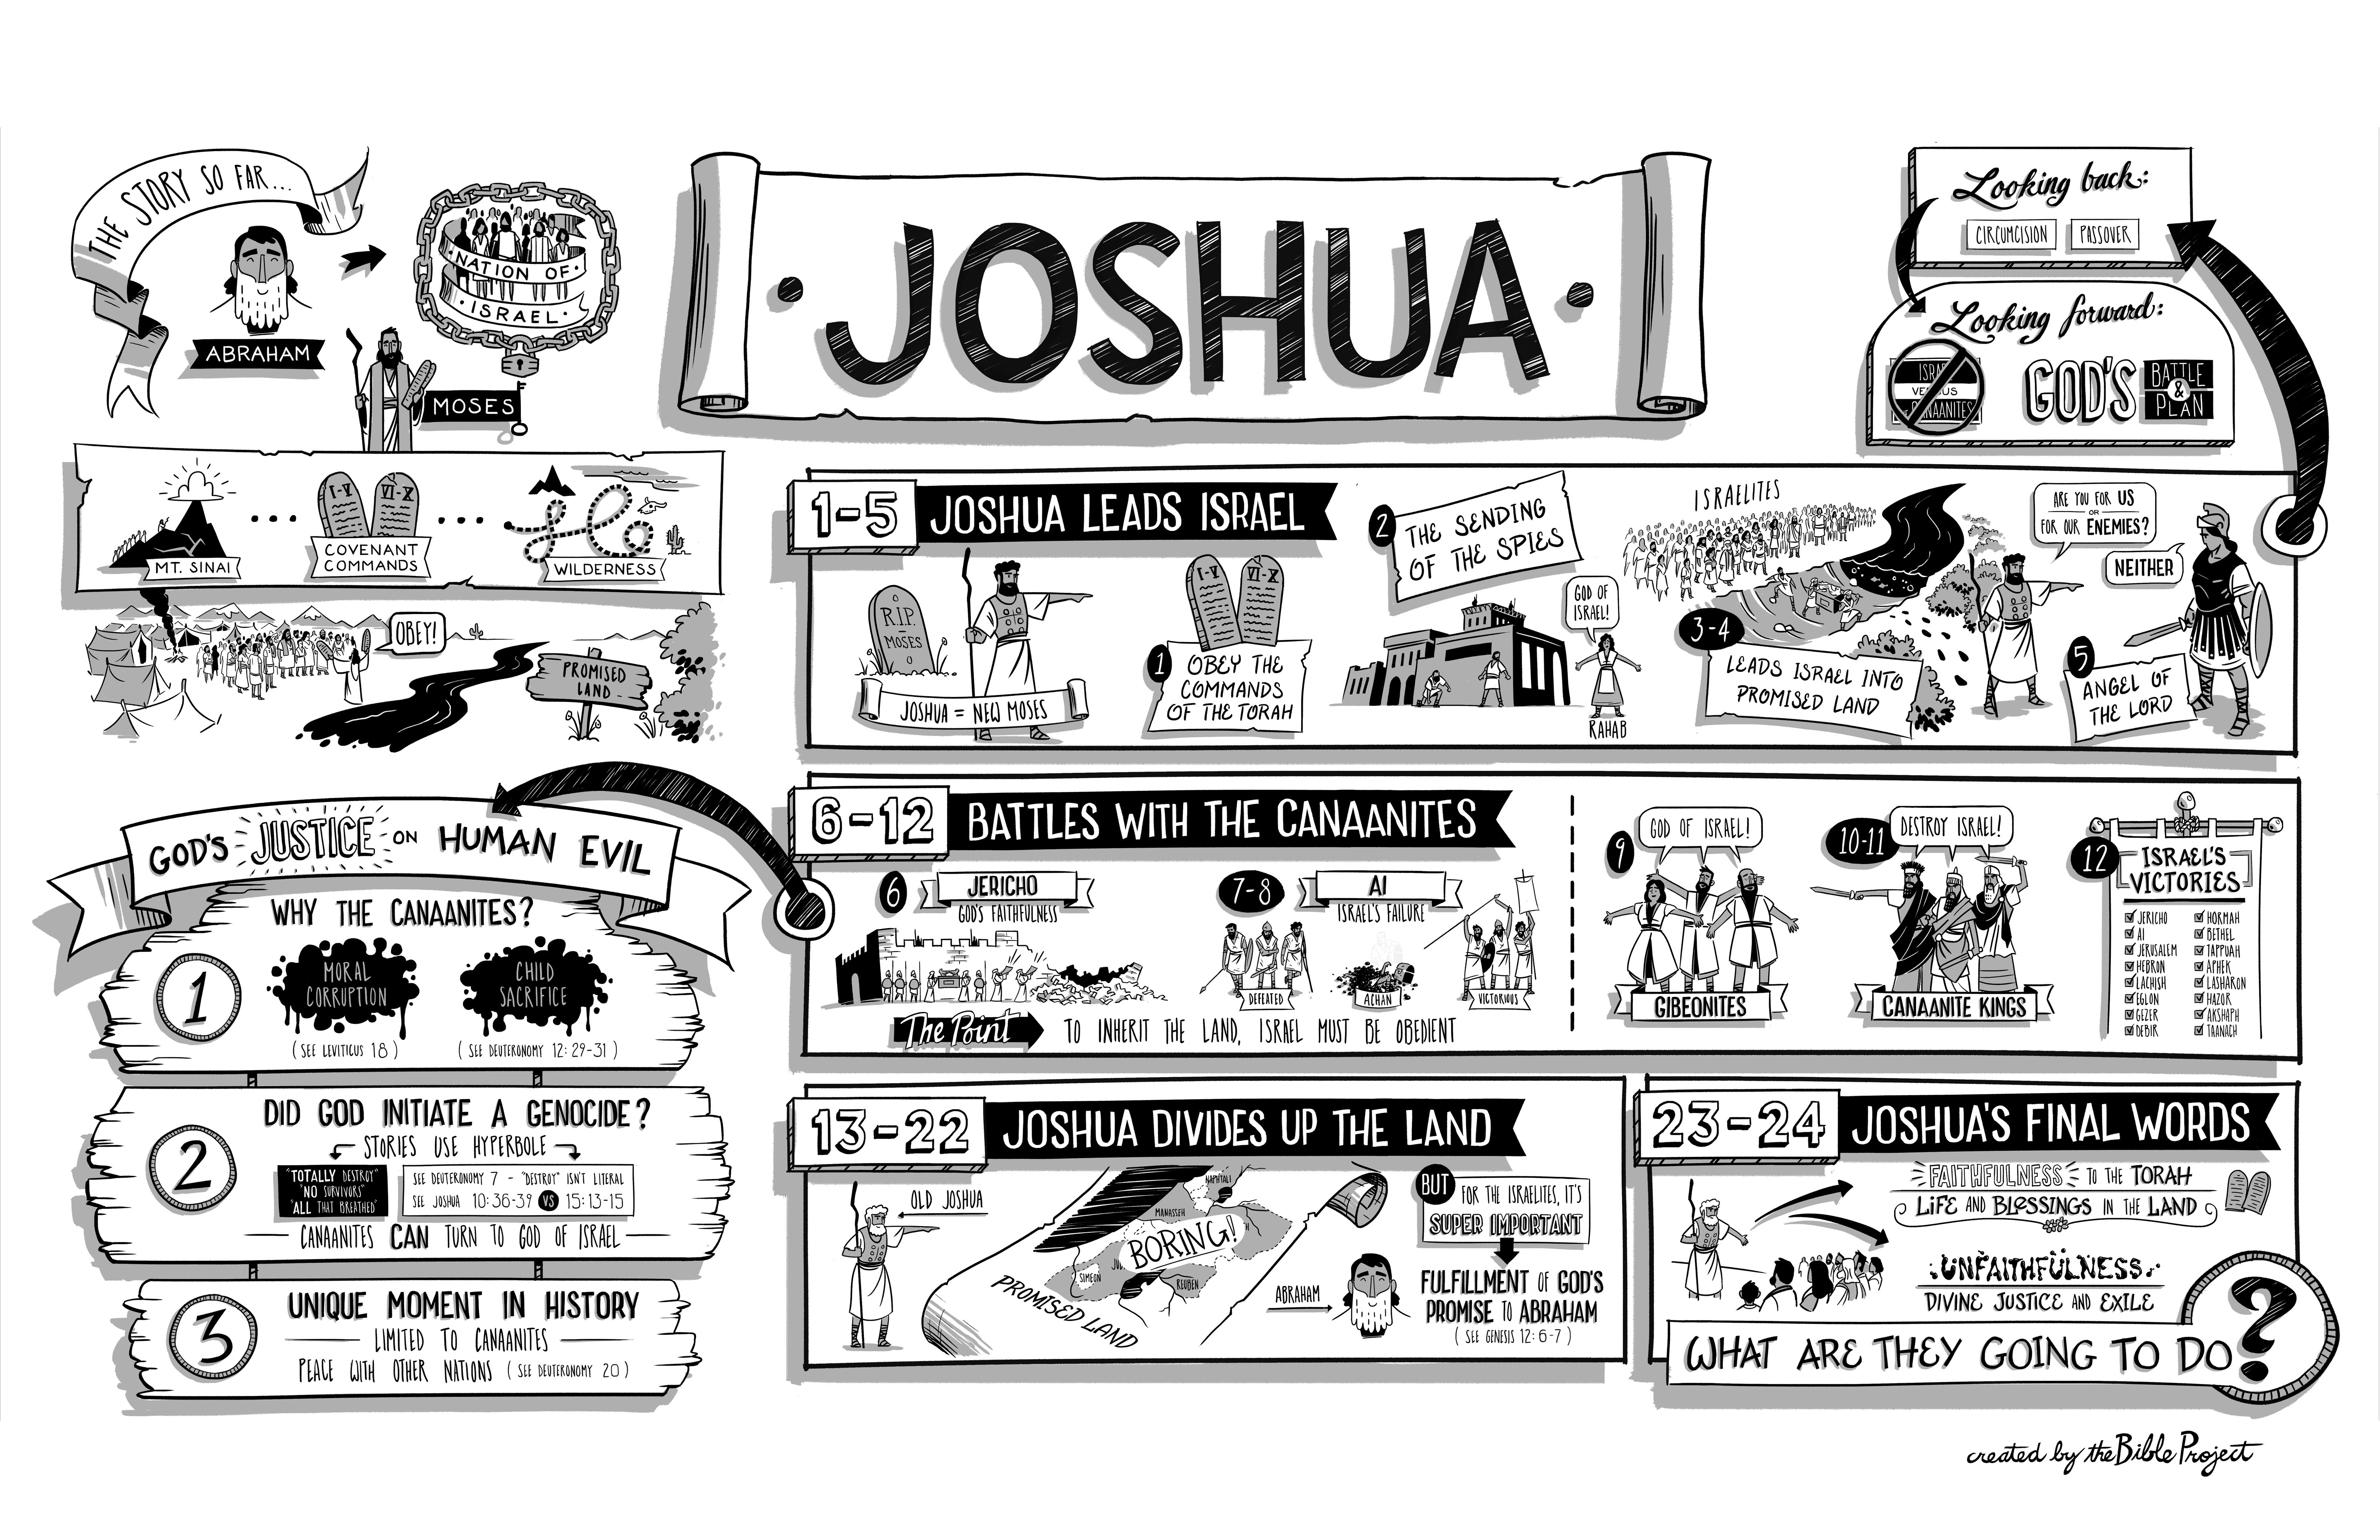
\includegraphics[scale=0.5, angle=90]{06OT-Joshua/References/1.BibleProject-Joshua.jpg}
\caption[Joshua from the Bible Project]{Joshua from the Bible Project}
\label{fig:Joshua from the Bible Project}
\end{center}
\end{figure}

\newpage
\begin{figure}
\begin{center}
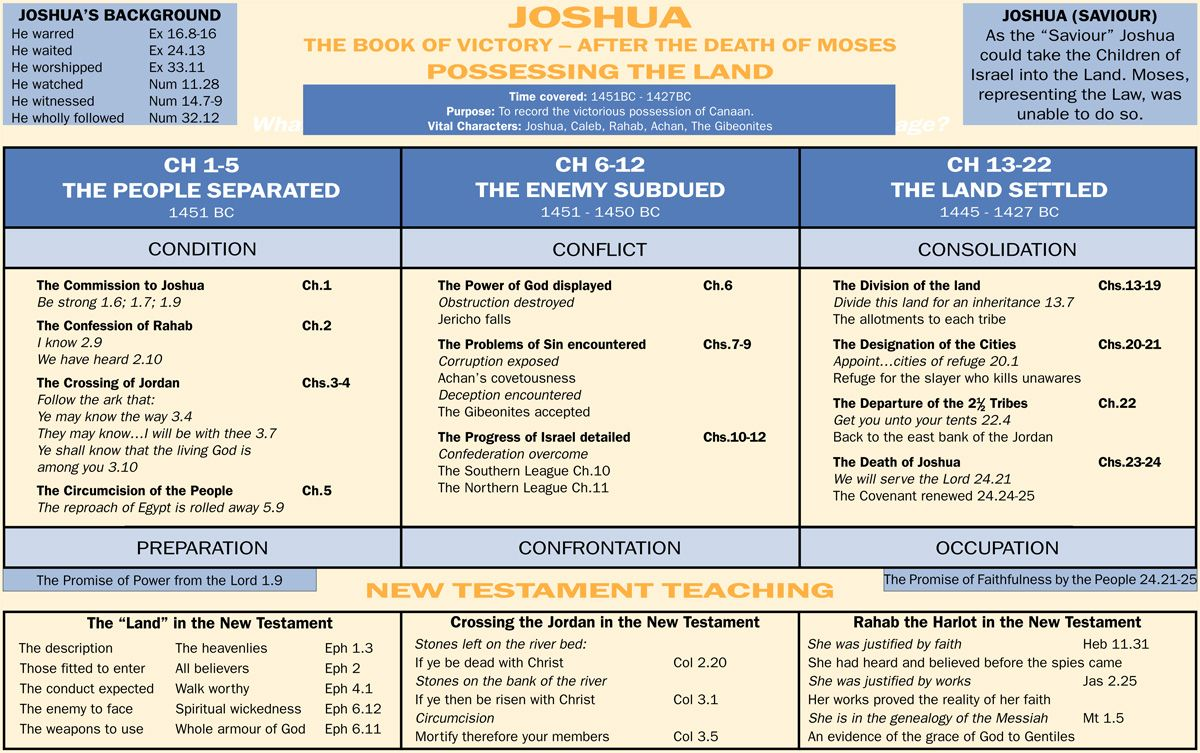
\includegraphics[scale=0.5, angle=90]{06OT-Joshua/References/2.JohnGrant-Joshua.jpg}
\caption[Joshua from John Grant]{Joshua from John Grant}
\label{fig:Joshua from John Grant}
\end{center}
\end{figure}

\newpage
\begin{figure}
\begin{center}
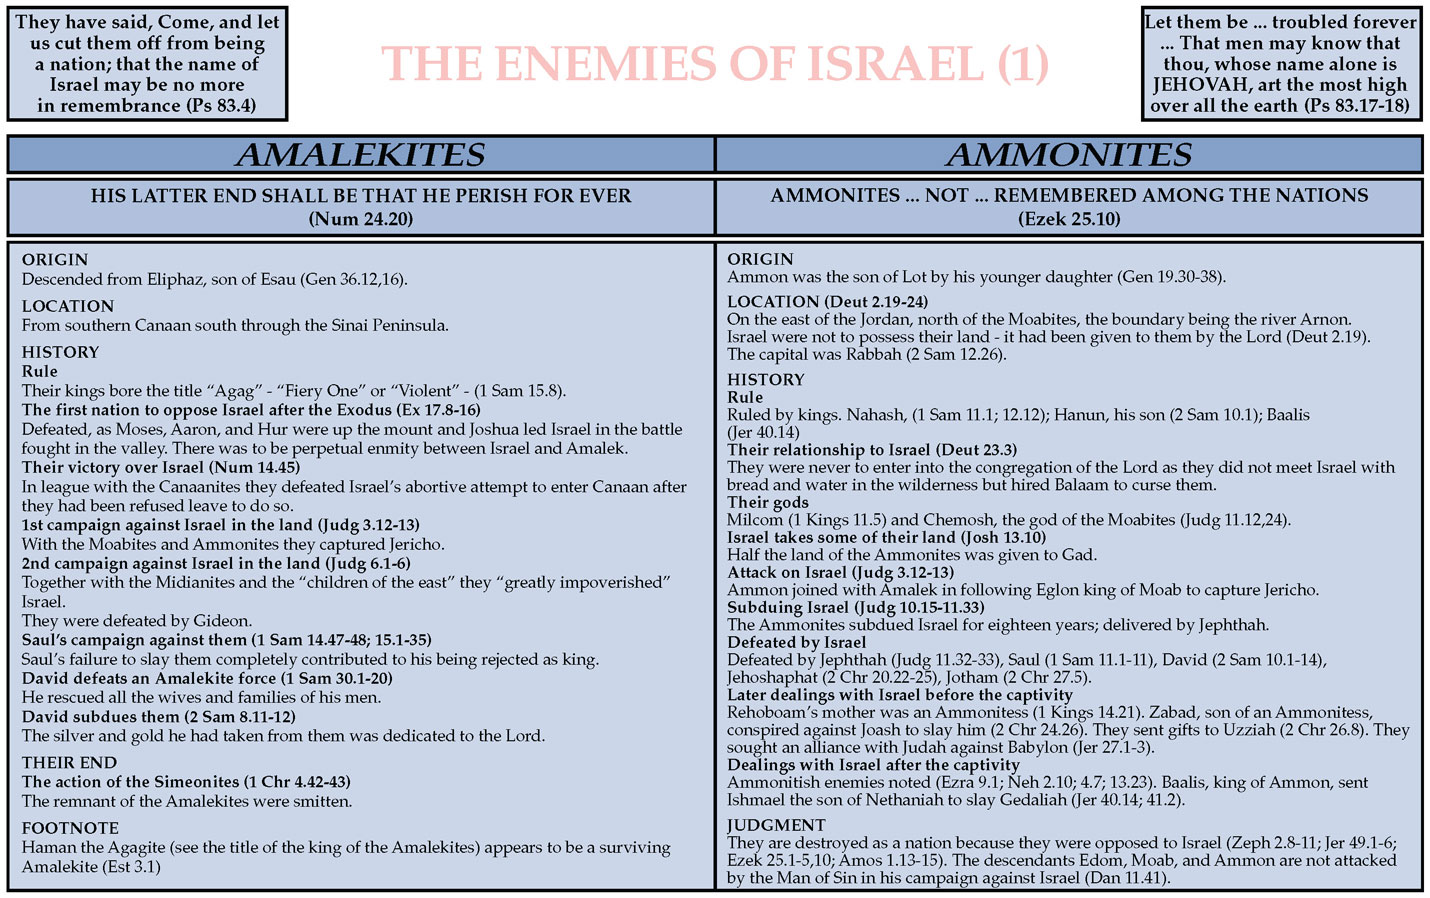
\includegraphics[scale=0.4, angle=90]{06OT-Joshua/References/3.EnemiesOfIsrael1.jpg}
\caption[Enemies of Israel 1]{Enemies of Israel 1}
\label{fig:Enemies of Israel 1}
\end{center}
\end{figure}

\newpage
\begin{figure}
\begin{center}
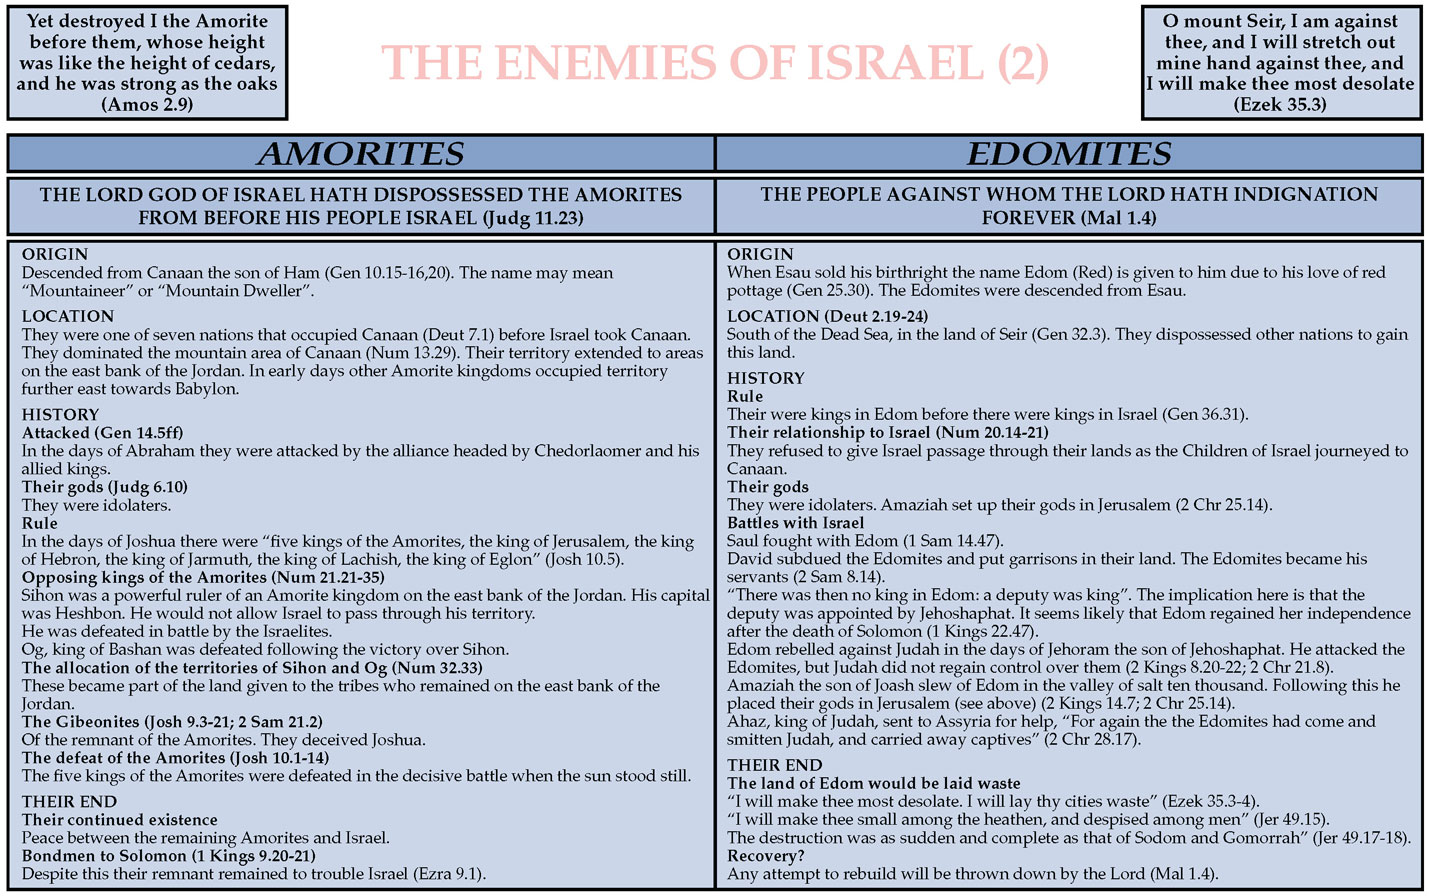
\includegraphics[scale=0.4, angle=90]{06OT-Joshua/References/4.EnemiesOfIsrael2.jpg}
\caption[Enemies of Israel 2]{Enemies of Israel 2}
\label{fig:Enemies of Israel 2}
\end{center}
\end{figure}

\newpage
\begin{figure}
\begin{center}
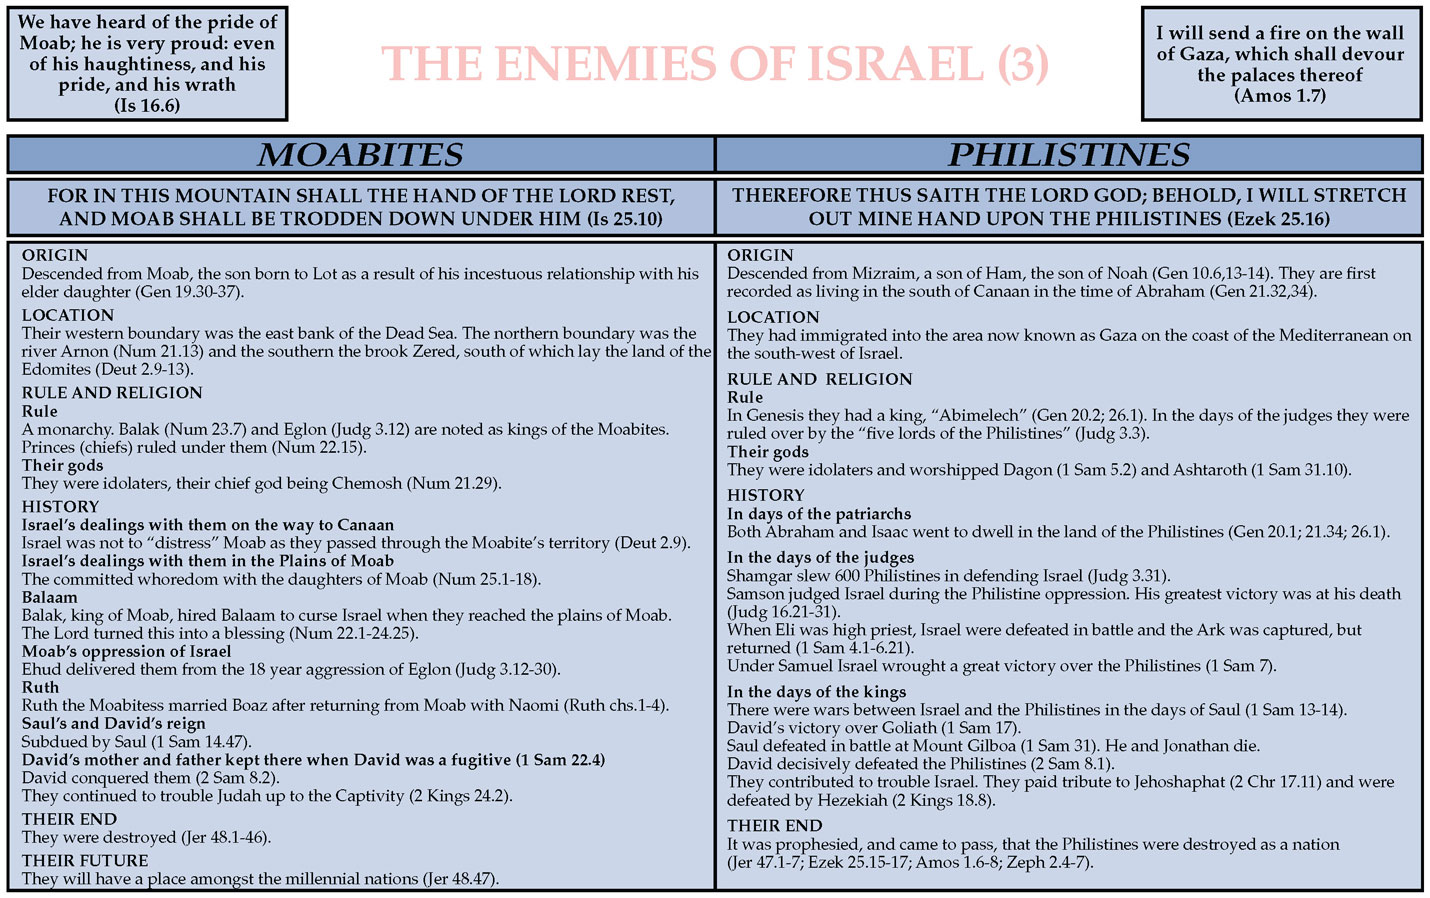
\includegraphics[scale=0.4, angle=90]{06OT-Joshua/References/5.EnemiesOfIsrael3.jpg}
\caption[Enemies of Israel 3]{Enemies of Israel 3}
\label{fig:Enemies of Israel 3}
\end{center}
\end{figure}

\newpage
\begin{figure}
\begin{center}
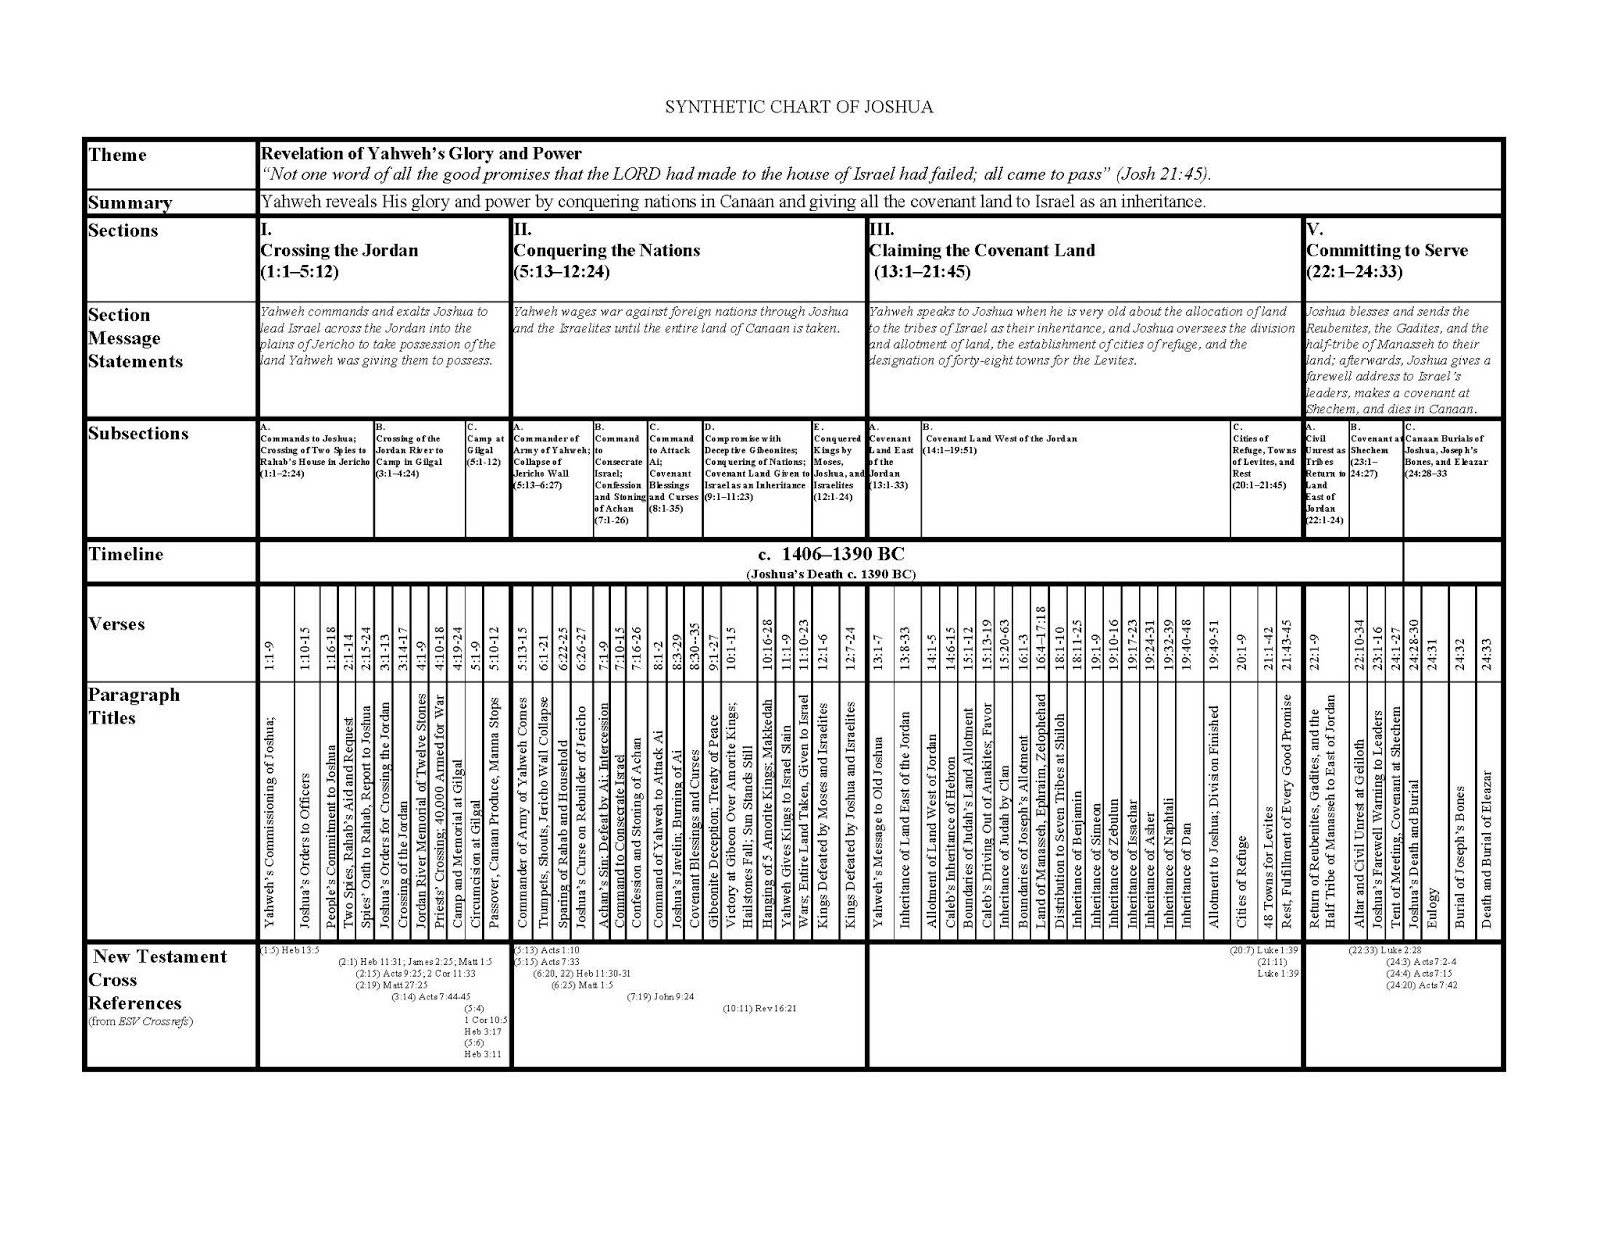
\includegraphics[scale=.4, angle=90]{06OT-Joshua/References/6.SyntheticChartofJoshua.jpg}
\caption[Synthetic Chart of Joshua]{Synthetic Chart of Joshua}
\label{fig:Synthetic Chart of Joshua}
\end{center}
\end{figure}


\newpage
\begin{figure}
\begin{center}
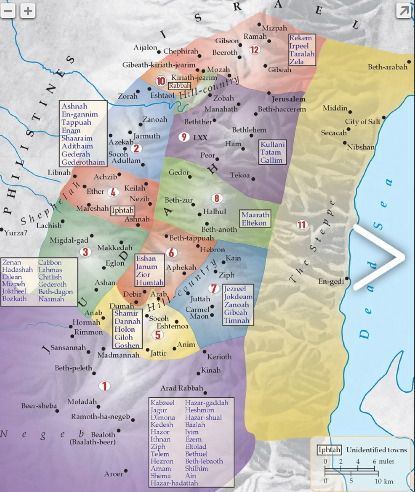
\includegraphics[scale=1, angle=0]{06OT-Joshua/References/7.WestSideOfDeadSea.jpg}
\caption[The West Side of the Dead Sea]{The West Side of the Dead Sea}
\label{fig:The West Side of the Dead Sea}
\end{center}
\end{figure}


\newpage
\begin{figure}
\begin{center}
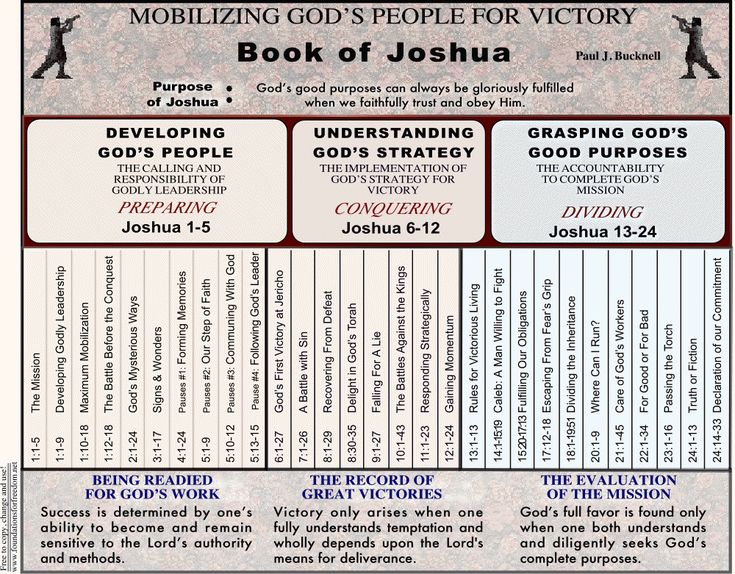
\includegraphics[scale=0.75, angle=90]{06OT-Joshua/References/8.Bucknell-Joshua.jpg}
\caption[Joshua from Bucknell]{Joshua from Bucknell}
\label{fig:Joshua from Bucknell}
\end{center}
\end{figure}


\newpage
\begin{figure}
\begin{center}
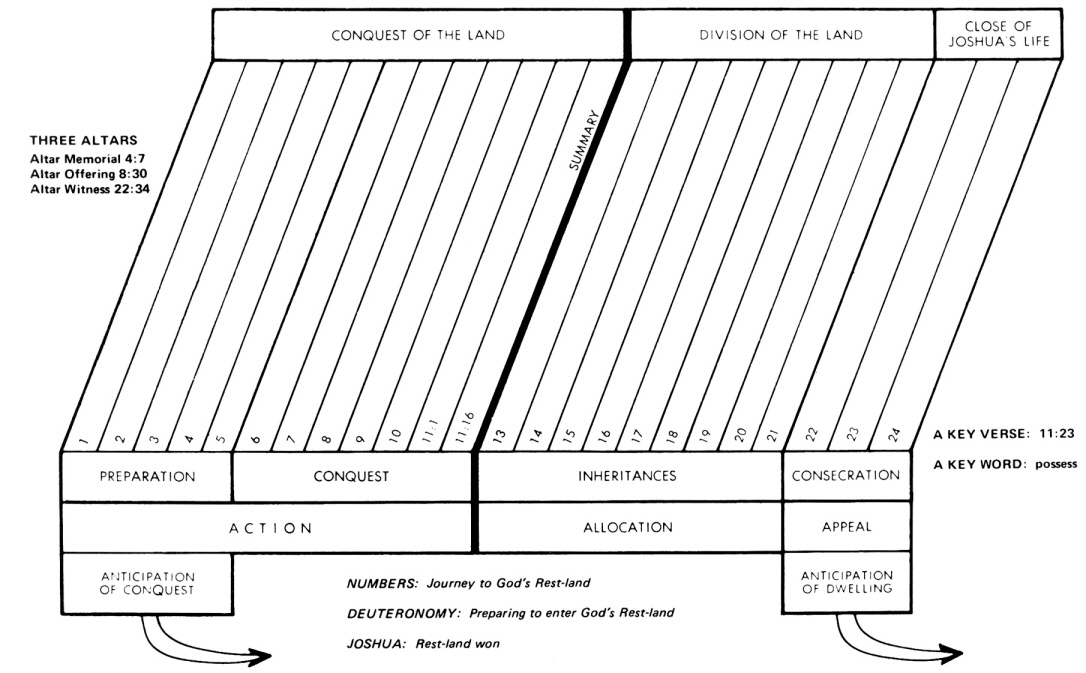
\includegraphics[scale=2, angle=90]{06OT-Joshua/References/9.Jensen-Joshua.png}
\caption[Joshua from Jensen]{Joshua from Jensen}
\label{fig:Joshua from Jensen}
\end{center}
\end{figure}


\newpage
\begin{figure}
\begin{center}
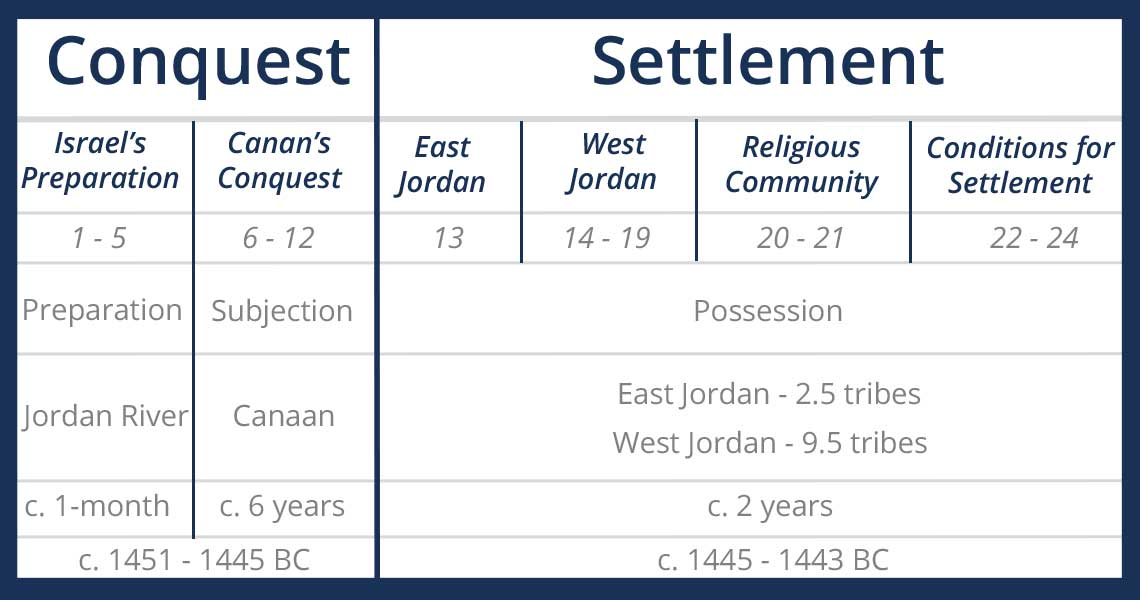
\includegraphics[scale=.5, angle=90]{06OT-Joshua/References/10.Bible-Brief-Joshua.jpg}
\caption[Bible Brief for Joshua]{Bible Brief for Joshua}
\label{fig:Bible Brief for Joshua}
\end{center}
\end{figure}

\newpage
\begin{figure}
\begin{center}
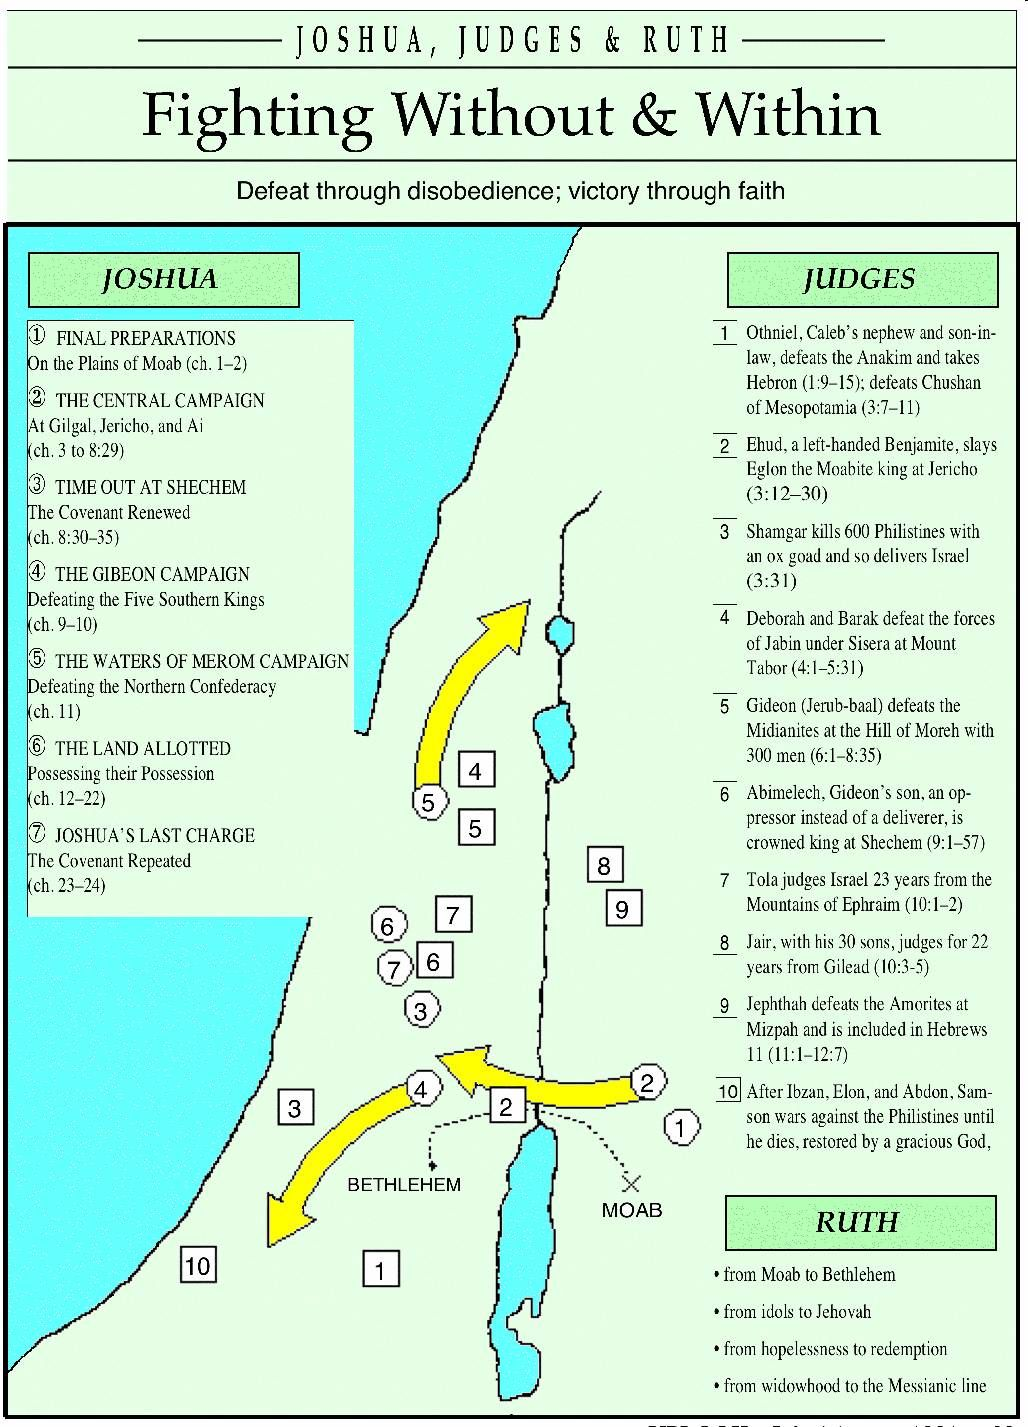
\includegraphics[scale=.5, angle=0]{06OT-Joshua/References/11.FightingInJoshuaAndJudges.jpg}
\caption[The Fighting in Joshua and Judges]{The Fighting in Joshua and Judges}
\label{fig:The Fighting in Joshua and Judges}
\end{center}
\end{figure}

\newpage
\begin{figure}
\begin{center}
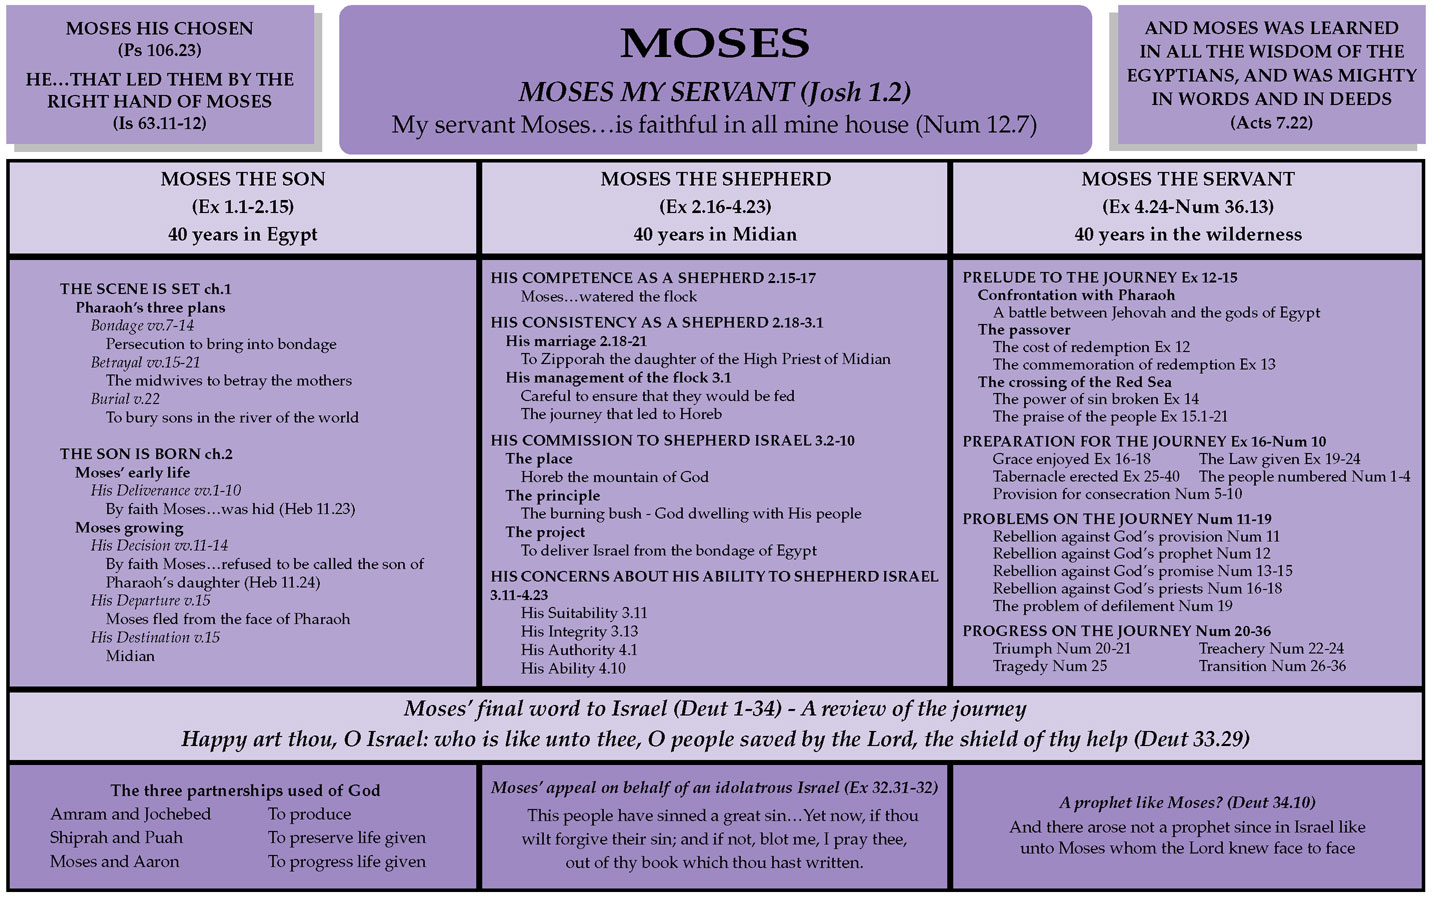
\includegraphics[scale=.4, angle=90]{06OT-Joshua/References/12.JohnGrantMoses.jpg}
\caption[Moses from John Grant]{Moses from John Grant}
\label{fig:Moses from John Grant}
\end{center}
\end{figure}







\chapter{Joshua 22}

% \textcolor[cmyk]{0.99998,1,0,0}{
\marginpar{\scriptsize \centering \fcolorbox{bone}{lime}{\textbf{BACK TO THE OTHER SIDE}}\\ (Joshua 22)

\begin{compactenum}[I.][8]

    \item The \textbf{Two-and-a-Half} \index[scripture]{Joshua!Jsh 22:01}(Jsh 22:1)
    \item \textbf{Toward the East} \index[scripture]{Joshua!Jsh 22:05}(Jsh 22:5)
    \item \textbf{Trouble at Church} \index[scripture]{Joshua!Jsh 22:11}(Jsh 22:11)
    \item \textbf{Tension} \index[scripture]{Joshua!Jsh 22:12}(Jsh 22:12)
    \item A \textbf{Testimony to Unity} \index[scripture]{Joshua!Jsh 22:27}(Jsh 22:27)

\end{compactenum}}

\footnote{\textcolor[rgb]{0.00,0.25,0.00}{\hyperlink{TOC}{Return to end of Table of Contents.}}}\footnote{\href{https://audiobible.com/bible/joshua_22.html}{\textcolor[cmyk]{0.99998,1,0,0}{Joshua 22 Audio}}}\textcolor[cmyk]{0.99998,1,0,0}{Then Joshua called the Reubenites, and the Gadites, and the half tribe of Manasseh,}
[2] \textcolor[cmyk]{0.99998,1,0,0}{And said unto them, Ye have kept all that Moses the servant \fcolorbox{bone}{bone}{of the LORD} commanded you, and have obeyed my voice in all that I commanded you:}
[3] \textcolor[cmyk]{0.99998,1,0,0}{Ye have not left your brethren these many days unto this day, but have kept the charge of the commandment \fcolorbox{bone}{bone}{of the LORD} your God.}
[4] \textcolor[cmyk]{0.99998,1,0,0}{And now the LORD your God hath given rest unto your brethren, as he promised them: therefore now return ye, and get you unto your tents, \emph{and} unto the land of your possession, which Moses the servant \fcolorbox{bone}{bone}{of the LORD} gave you on the other side Jordan.}
[5] \textcolor[cmyk]{0.99998,1,0,0}{But take diligent heed to do the commandment and the law, which Moses the servant \fcolorbox{bone}{bone}{of the LORD} charged you, to love the LORD your God, and to walk in all his ways, and to keep his commandments, and to cleave unto him, and to serve him with all your heart and with all your soul.}
[6] \textcolor[cmyk]{0.99998,1,0,0}{So Joshua blessed them, and sent them away: and they went unto their tents.}\\
\\
\P \textcolor[cmyk]{0.99998,1,0,0}{Now to the \emph{one} half of the tribe of Manasseh Moses had given \emph{possession} in Bashan: but unto the \emph{other} half thereof gave Joshua among their brethren on this side Jordan westward. And when Joshua sent them away also unto their tents, then he blessed them,}
[8] \textcolor[cmyk]{0.99998,1,0,0}{And he spake unto them, saying, Return with much riches unto your tents, and with very much cattle, with silver, and with gold, and with brass, and with iron, and with very much raiment: divide the spoil of your enemies with your brethren.}\\
\\
\P \textcolor[cmyk]{0.99998,1,0,0}{And the children of Reuben and the children of Gad and the half tribe of Manasseh returned, and departed from the children of Israel out of Shiloh, which \emph{is} in the land of Canaan, to go unto the country of Gilead, to the land of their possession, whereof they were possessed, according to the word \fcolorbox{bone}{bone}{of the LORD} by the hand of Moses.}\\
\\
\P \textcolor[cmyk]{0.99998,1,0,0}{And when they came unto the borders of Jordan, that \emph{are} in the land of Canaan, the children of Reuben and the children of Gad and the half tribe of Manasseh built there an altar by Jordan, a great altar to see to.}\\
\\
\P \textcolor[cmyk]{0.99998,1,0,0}{And the children of Israel heard say, Behold, the children of Reuben and the children of Gad and the half tribe of Manasseh have built an altar over against the land of Canaan, in the borders of Jordan, at the passage of the children of Israel.}
[12] \textcolor[cmyk]{0.99998,1,0,0}{And when the children of Israel heard \emph{of} \emph{it}, the whole congregation of the children of Israel gathered themselves together at Shiloh, to go up to war against them.}
[13] \textcolor[cmyk]{0.99998,1,0,0}{And the children of Israel sent unto the children of Reuben, and to the children of Gad, and to the half tribe of Manasseh, into the land of Gilead, Phinehas the son of Eleazar the priest,}
[14] \textcolor[cmyk]{0.99998,1,0,0}{And with him ten princes, of each chief house a prince throughout all the tribes of Israel; and each one \emph{was} an head of the house of their fathers among the thousands of Israel.}\\
\\
\P \textcolor[cmyk]{0.99998,1,0,0}{And they came unto the children of Reuben, and to the children of Gad, and to the half tribe of Manasseh, unto the land of Gilead, and they spake with them, saying,}
[16] \textcolor[cmyk]{0.99998,1,0,0}{Thus saith the whole congregation \fcolorbox{bone}{bone}{of the LORD}, What trespass \emph{is} this that ye have committed against the God of Israel, to turn away this day from following the LORD, in that ye have builded you an altar, that ye might rebel this day against the LORD?}
[17] \textcolor[cmyk]{0.99998,1,0,0}{\emph{Is} the iniquity of Peor too little for us, from which we are not cleansed until this day, although there was a plague in the congregation \fcolorbox{bone}{bone}{of the LORD},}
[18] \textcolor[cmyk]{0.99998,1,0,0}{But that ye must turn away this day from following the LORD? and it will be, \emph{seeing} ye rebel to day against the LORD, that to morrow he will be wroth with the whole congregation of Israel.}
[19] \textcolor[cmyk]{0.99998,1,0,0}{Notwithstanding, if the land of your possession \emph{be} unclean, \emph{then} pass ye over unto the land of the possession \fcolorbox{bone}{bone}{of the LORD}, wherein the LORD'S tabernacle dwelleth, and take possession among us: but rebel not against the LORD, nor rebel against us, in building you an altar beside the altar \fcolorbox{bone}{bone}{of the LORD} our God.}
[20] \textcolor[cmyk]{0.99998,1,0,0}{Did not Achan the son of Zerah commit a trespass in the accursed thing, and wrath fell on all the congregation of Israel? and that man perished not alone in his iniquity.}\\
\\
\P \textcolor[cmyk]{0.99998,1,0,0}{Then the children of Reuben and the children of Gad and the half tribe of Manasseh answered, and said unto the heads of the thousands of Israel,}
[22] \textcolor[cmyk]{0.99998,1,0,0}{The LORD God of gods, the LORD God of gods, he knoweth, and Israel he shall know; if \emph{it} \emph{be} in rebellion, or if in \fcolorbox{bone}{MYGOLD}{transgression} against the LORD, (save us not this day,)}
[23] \textcolor[cmyk]{0.99998,1,0,0}{That we have built us an altar to turn from following the LORD, or if to offer thereon burnt offering or meat offering, or if to offer peace offerings thereon, let the LORD himself require \emph{it};}
[24] \textcolor[cmyk]{0.99998,1,0,0}{And if we have not \emph{rather} done it for fear of \emph{this} thing, saying, In time to come your children might speak unto our children, saying, What have ye to do with the LORD God of Israel?}
[25] \textcolor[cmyk]{0.99998,1,0,0}{For the LORD hath made Jordan a border between us and you, ye children of Reuben and children of Gad; ye have no part in the LORD: so shall your children make our children cease from fearing the LORD.}
[26] \textcolor[cmyk]{0.99998,1,0,0}{Therefore we said, Let us now prepare to build us an altar, not for burnt offering, nor for sacrifice:}
[27] \textcolor[cmyk]{0.99998,1,0,0}{But \emph{that} it \emph{may} \emph{be} a witness between us, and you, and our generations after us, that we might do the service \fcolorbox{bone}{bone}{of the LORD} before him with our burnt offerings, and with our sacrifices, and with our peace offerings; that your children may not say to our children in time to come, Ye have no part in the LORD.}
[28] \textcolor[cmyk]{0.99998,1,0,0}{Therefore said we, that it shall be, when they should \emph{so} say to us or to our generations in time to come, that we may say \emph{again}, Behold the pattern of the altar \fcolorbox{bone}{bone}{of the LORD}, which our fathers made, not for burnt offerings, nor for sacrifices; but it \emph{is} a witness between us and you.}
[29] \textcolor[cmyk]{0.99998,1,0,0}{God forbid that we should rebel against the LORD, and turn this day from following the LORD, to build an altar for burnt offerings, for meat offerings, or for sacrifices, beside the altar \fcolorbox{bone}{bone}{of the LORD} our God that \emph{is} before his tabernacle.}\\
\\
\P \textcolor[cmyk]{0.99998,1,0,0}{And when Phinehas the priest, and the princes of the congregation and heads of the thousands of Israel which \emph{were} with him, heard the words that the children of Reuben and the children of Gad and the children of Manasseh spake, it pleased them.}
[31] \textcolor[cmyk]{0.99998,1,0,0}{And Phinehas the son of Eleazar the priest said unto the children of Reuben, and to the children of Gad, and to the children of Manasseh, This day we perceive that the LORD \emph{is} among us, because ye have not committed this trespass against the LORD: now ye have delivered the children of Israel out of the hand \fcolorbox{bone}{bone}{of the LORD}.}\\
\\
\P \textcolor[cmyk]{0.99998,1,0,0}{And Phinehas the son of Eleazar the priest, and the princes, returned from the children of Reuben, and from the children of Gad, out of the land of Gilead, unto the land of Canaan, to the children of Israel, and brought them word again.}
[33] \textcolor[cmyk]{0.99998,1,0,0}{And the thing pleased the children of Israel; and the children of Israel blessed God, and did not intend to go up against them in battle, to destroy the land wherein the children of Reuben and Gad dwelt.}
[34] \textcolor[cmyk]{0.99998,1,0,0}{And the children of Reuben and the children of Gad called the altar \emph{Ed}: for it \emph{shall} \emph{be} a witness between us that the LORD \emph{is} God.}
\index[NWIV]{14!Joshua!Jos 22:1}\index[AWIP]{Then!Joshua!Jos 22:1}\index[AWIP]{Joshua!Joshua!Jos 22:1}\index[AWIP]{called!Joshua!Jos 22:1}\index[AWIP]{the!Joshua!Jos 22:1}\index[AWIP]{the!Joshua!Jos 22:1 (2)}\index[AWIP]{the!Joshua!Jos 22:1 (3)}\index[AWIP]{Reubenites!Joshua!Jos 22:1}\index[AWIP]{and!Joshua!Jos 22:1}\index[AWIP]{and!Joshua!Jos 22:1 (2)}\index[AWIP]{Gadites!Joshua!Jos 22:1}\index[AWIP]{half!Joshua!Jos 22:1}\index[AWIP]{tribe!Joshua!Jos 22:1}\index[AWIP]{of!Joshua!Jos 22:1}\index[AWIP]{Manasseh!Joshua!Jos 22:1}

\index[NWIV]{28!Joshua!Jos 22:2}\index[AWIP]{And!Joshua!Jos 22:2}\index[AWIP]{said!Joshua!Jos 22:2}\index[AWIP]{unto!Joshua!Jos 22:2}\index[AWIP]{them!Joshua!Jos 22:2}\index[AWIP]{Ye!Joshua!Jos 22:2}\index[AWIP]{have!Joshua!Jos 22:2}\index[AWIP]{have!Joshua!Jos 22:2 (2)}\index[AWIP]{kept!Joshua!Jos 22:2}\index[AWIP]{all!Joshua!Jos 22:2}\index[AWIP]{all!Joshua!Jos 22:2 (2)}\index[AWIP]{that!Joshua!Jos 22:2}\index[AWIP]{that!Joshua!Jos 22:2 (2)}\index[AWIP]{Moses!Joshua!Jos 22:2}\index[AWIP]{the!Joshua!Jos 22:2}\index[AWIP]{the!Joshua!Jos 22:2 (2)}\index[AWIP]{servant!Joshua!Jos 22:2}\index[AWIP]{of!Joshua!Jos 22:2}\index[AWIP]{LORD!Joshua!Jos 22:2}\index[AWIP]{commanded!Joshua!Jos 22:2}\index[AWIP]{commanded!Joshua!Jos 22:2 (2)}\index[AWIP]{you!Joshua!Jos 22:2}\index[AWIP]{you!Joshua!Jos 22:2 (2)}\index[AWIP]{and!Joshua!Jos 22:2}\index[AWIP]{obeyed!Joshua!Jos 22:2}\index[AWIP]{my!Joshua!Jos 22:2}\index[AWIP]{voice!Joshua!Jos 22:2}\index[AWIP]{in!Joshua!Jos 22:2}\index[AWIP]{I!Joshua!Jos 22:2}

\index[NWIV]{25!Joshua!Jos 22:3}\index[AWIP]{Ye!Joshua!Jos 22:3}\index[AWIP]{have!Joshua!Jos 22:3}\index[AWIP]{have!Joshua!Jos 22:3 (2)}\index[AWIP]{not!Joshua!Jos 22:3}\index[AWIP]{left!Joshua!Jos 22:3}\index[AWIP]{your!Joshua!Jos 22:3}\index[AWIP]{your!Joshua!Jos 22:3 (2)}\index[AWIP]{brethren!Joshua!Jos 22:3}\index[AWIP]{these!Joshua!Jos 22:3}\index[AWIP]{many!Joshua!Jos 22:3}\index[AWIP]{days!Joshua!Jos 22:3}\index[AWIP]{unto!Joshua!Jos 22:3}\index[AWIP]{this!Joshua!Jos 22:3}\index[AWIP]{day!Joshua!Jos 22:3}\index[AWIP]{but!Joshua!Jos 22:3}\index[AWIP]{kept!Joshua!Jos 22:3}\index[AWIP]{the!Joshua!Jos 22:3}\index[AWIP]{the!Joshua!Jos 22:3 (2)}\index[AWIP]{the!Joshua!Jos 22:3 (3)}\index[AWIP]{charge!Joshua!Jos 22:3}\index[AWIP]{of!Joshua!Jos 22:3}\index[AWIP]{of!Joshua!Jos 22:3 (2)}\index[AWIP]{commandment!Joshua!Jos 22:3}\index[AWIP]{LORD!Joshua!Jos 22:3}\index[AWIP]{God!Joshua!Jos 22:3}

\index[NWIV]{47!Joshua!Jos 22:4}\index[AWIP]{And!Joshua!Jos 22:4}\index[AWIP]{now!Joshua!Jos 22:4}\index[AWIP]{now!Joshua!Jos 22:4 (2)}\index[AWIP]{the!Joshua!Jos 22:4}\index[AWIP]{the!Joshua!Jos 22:4 (2)}\index[AWIP]{the!Joshua!Jos 22:4 (3)}\index[AWIP]{the!Joshua!Jos 22:4 (4)}\index[AWIP]{the!Joshua!Jos 22:4 (5)}\index[AWIP]{LORD!Joshua!Jos 22:4}\index[AWIP]{LORD!Joshua!Jos 22:4 (2)}\index[AWIP]{your!Joshua!Jos 22:4}\index[AWIP]{your!Joshua!Jos 22:4 (2)}\index[AWIP]{your!Joshua!Jos 22:4 (3)}\index[AWIP]{your!Joshua!Jos 22:4 (4)}\index[AWIP]{God!Joshua!Jos 22:4}\index[AWIP]{hath!Joshua!Jos 22:4}\index[AWIP]{given!Joshua!Jos 22:4}\index[AWIP]{rest!Joshua!Jos 22:4}\index[AWIP]{unto!Joshua!Jos 22:4}\index[AWIP]{unto!Joshua!Jos 22:4 (2)}\index[AWIP]{unto!Joshua!Jos 22:4 (3)}\index[AWIP]{brethren!Joshua!Jos 22:4}\index[AWIP]{as!Joshua!Jos 22:4}\index[AWIP]{he!Joshua!Jos 22:4}\index[AWIP]{promised!Joshua!Jos 22:4}\index[AWIP]{them!Joshua!Jos 22:4}\index[AWIP]{therefore!Joshua!Jos 22:4}\index[AWIP]{return!Joshua!Jos 22:4}\index[AWIP]{ye!Joshua!Jos 22:4}\index[AWIP]{and!Joshua!Jos 22:4}\index[AWIP]{get!Joshua!Jos 22:4}\index[AWIP]{you!Joshua!Jos 22:4}\index[AWIP]{you!Joshua!Jos 22:4 (2)}\index[AWIP]{tents!Joshua!Jos 22:4}\index[AWIP]{\emph{and}!Joshua!Jos 22:4}\index[AWIP]{land!Joshua!Jos 22:4}\index[AWIP]{of!Joshua!Jos 22:4}\index[AWIP]{of!Joshua!Jos 22:4 (2)}\index[AWIP]{possession!Joshua!Jos 22:4}\index[AWIP]{which!Joshua!Jos 22:4}\index[AWIP]{Moses!Joshua!Jos 22:4}\index[AWIP]{servant!Joshua!Jos 22:4}\index[AWIP]{gave!Joshua!Jos 22:4}\index[AWIP]{on!Joshua!Jos 22:4}\index[AWIP]{other!Joshua!Jos 22:4}\index[AWIP]{side!Joshua!Jos 22:4}\index[AWIP]{Jordan!Joshua!Jos 22:4}\index[AWIP]{\emph{and}!Joshua!Jos 22:4}

\index[NWIV]{56!Joshua!Jos 22:5}\index[AWIP]{But!Joshua!Jos 22:5}\index[AWIP]{take!Joshua!Jos 22:5}\index[AWIP]{diligent!Joshua!Jos 22:5}\index[AWIP]{heed!Joshua!Jos 22:5}\index[AWIP]{to!Joshua!Jos 22:5}\index[AWIP]{to!Joshua!Jos 22:5 (2)}\index[AWIP]{to!Joshua!Jos 22:5 (3)}\index[AWIP]{to!Joshua!Jos 22:5 (4)}\index[AWIP]{to!Joshua!Jos 22:5 (5)}\index[AWIP]{to!Joshua!Jos 22:5 (6)}\index[AWIP]{do!Joshua!Jos 22:5}\index[AWIP]{the!Joshua!Jos 22:5}\index[AWIP]{the!Joshua!Jos 22:5 (2)}\index[AWIP]{the!Joshua!Jos 22:5 (3)}\index[AWIP]{the!Joshua!Jos 22:5 (4)}\index[AWIP]{the!Joshua!Jos 22:5 (5)}\index[AWIP]{commandment!Joshua!Jos 22:5}\index[AWIP]{and!Joshua!Jos 22:5}\index[AWIP]{and!Joshua!Jos 22:5 (2)}\index[AWIP]{and!Joshua!Jos 22:5 (3)}\index[AWIP]{and!Joshua!Jos 22:5 (4)}\index[AWIP]{and!Joshua!Jos 22:5 (5)}\index[AWIP]{and!Joshua!Jos 22:5 (6)}\index[AWIP]{law!Joshua!Jos 22:5}\index[AWIP]{which!Joshua!Jos 22:5}\index[AWIP]{Moses!Joshua!Jos 22:5}\index[AWIP]{servant!Joshua!Jos 22:5}\index[AWIP]{of!Joshua!Jos 22:5}\index[AWIP]{LORD!Joshua!Jos 22:5}\index[AWIP]{LORD!Joshua!Jos 22:5 (2)}\index[AWIP]{charged!Joshua!Jos 22:5}\index[AWIP]{you!Joshua!Jos 22:5}\index[AWIP]{love!Joshua!Jos 22:5}\index[AWIP]{your!Joshua!Jos 22:5}\index[AWIP]{your!Joshua!Jos 22:5 (2)}\index[AWIP]{your!Joshua!Jos 22:5 (3)}\index[AWIP]{God!Joshua!Jos 22:5}\index[AWIP]{walk!Joshua!Jos 22:5}\index[AWIP]{in!Joshua!Jos 22:5}\index[AWIP]{all!Joshua!Jos 22:5}\index[AWIP]{all!Joshua!Jos 22:5 (2)}\index[AWIP]{all!Joshua!Jos 22:5 (3)}\index[AWIP]{his!Joshua!Jos 22:5}\index[AWIP]{his!Joshua!Jos 22:5 (2)}\index[AWIP]{ways!Joshua!Jos 22:5}\index[AWIP]{keep!Joshua!Jos 22:5}\index[AWIP]{commandments!Joshua!Jos 22:5}\index[AWIP]{cleave!Joshua!Jos 22:5}\index[AWIP]{unto!Joshua!Jos 22:5}\index[AWIP]{him!Joshua!Jos 22:5}\index[AWIP]{him!Joshua!Jos 22:5 (2)}\index[AWIP]{serve!Joshua!Jos 22:5}\index[AWIP]{with!Joshua!Jos 22:5}\index[AWIP]{with!Joshua!Jos 22:5 (2)}\index[AWIP]{heart!Joshua!Jos 22:5}\index[AWIP]{soul!Joshua!Jos 22:5}

\index[NWIV]{14!Joshua!Jos 22:6}\index[AWIP]{So!Joshua!Jos 22:6}\index[AWIP]{Joshua!Joshua!Jos 22:6}\index[AWIP]{blessed!Joshua!Jos 22:6}\index[AWIP]{them!Joshua!Jos 22:6}\index[AWIP]{them!Joshua!Jos 22:6 (2)}\index[AWIP]{and!Joshua!Jos 22:6}\index[AWIP]{and!Joshua!Jos 22:6 (2)}\index[AWIP]{sent!Joshua!Jos 22:6}\index[AWIP]{away!Joshua!Jos 22:6}\index[AWIP]{they!Joshua!Jos 22:6}\index[AWIP]{went!Joshua!Jos 22:6}\index[AWIP]{unto!Joshua!Jos 22:6}\index[AWIP]{their!Joshua!Jos 22:6}\index[AWIP]{tents!Joshua!Jos 22:6}

\index[NWIV]{46!Joshua!Jos 22:7}\index[AWIP]{Now!Joshua!Jos 22:7}\index[AWIP]{to!Joshua!Jos 22:7}\index[AWIP]{the!Joshua!Jos 22:7}\index[AWIP]{the!Joshua!Jos 22:7 (2)}\index[AWIP]{the!Joshua!Jos 22:7 (3)}\index[AWIP]{\emph{one}!Joshua!Jos 22:7}\index[AWIP]{half!Joshua!Jos 22:7}\index[AWIP]{half!Joshua!Jos 22:7 (2)}\index[AWIP]{of!Joshua!Jos 22:7}\index[AWIP]{of!Joshua!Jos 22:7 (2)}\index[AWIP]{tribe!Joshua!Jos 22:7}\index[AWIP]{Manasseh!Joshua!Jos 22:7}\index[AWIP]{Moses!Joshua!Jos 22:7}\index[AWIP]{had!Joshua!Jos 22:7}\index[AWIP]{given!Joshua!Jos 22:7}\index[AWIP]{\emph{possession}!Joshua!Jos 22:7}\index[AWIP]{in!Joshua!Jos 22:7}\index[AWIP]{Bashan!Joshua!Jos 22:7}\index[AWIP]{but!Joshua!Jos 22:7}\index[AWIP]{unto!Joshua!Jos 22:7}\index[AWIP]{unto!Joshua!Jos 22:7 (2)}\index[AWIP]{\emph{other}!Joshua!Jos 22:7}\index[AWIP]{thereof!Joshua!Jos 22:7}\index[AWIP]{gave!Joshua!Jos 22:7}\index[AWIP]{Joshua!Joshua!Jos 22:7}\index[AWIP]{Joshua!Joshua!Jos 22:7 (2)}\index[AWIP]{among!Joshua!Jos 22:7}\index[AWIP]{their!Joshua!Jos 22:7}\index[AWIP]{their!Joshua!Jos 22:7 (2)}\index[AWIP]{brethren!Joshua!Jos 22:7}\index[AWIP]{on!Joshua!Jos 22:7}\index[AWIP]{this!Joshua!Jos 22:7}\index[AWIP]{side!Joshua!Jos 22:7}\index[AWIP]{Jordan!Joshua!Jos 22:7}\index[AWIP]{westward!Joshua!Jos 22:7}\index[AWIP]{And!Joshua!Jos 22:7}\index[AWIP]{when!Joshua!Jos 22:7}\index[AWIP]{sent!Joshua!Jos 22:7}\index[AWIP]{them!Joshua!Jos 22:7}\index[AWIP]{them!Joshua!Jos 22:7 (2)}\index[AWIP]{away!Joshua!Jos 22:7}\index[AWIP]{also!Joshua!Jos 22:7}\index[AWIP]{tents!Joshua!Jos 22:7}\index[AWIP]{then!Joshua!Jos 22:7}\index[AWIP]{he!Joshua!Jos 22:7}\index[AWIP]{blessed!Joshua!Jos 22:7}\index[AWIP]{\emph{one}!Joshua!Jos 22:7}\index[AWIP]{\emph{possession}!Joshua!Jos 22:7}\index[AWIP]{\emph{other}!Joshua!Jos 22:7}

\index[NWIV]{43!Joshua!Jos 22:8}\index[AWIP]{And!Joshua!Jos 22:8}\index[AWIP]{he!Joshua!Jos 22:8}\index[AWIP]{spake!Joshua!Jos 22:8}\index[AWIP]{unto!Joshua!Jos 22:8}\index[AWIP]{unto!Joshua!Jos 22:8 (2)}\index[AWIP]{them!Joshua!Jos 22:8}\index[AWIP]{saying!Joshua!Jos 22:8}\index[AWIP]{Return!Joshua!Jos 22:8}\index[AWIP]{with!Joshua!Jos 22:8}\index[AWIP]{with!Joshua!Jos 22:8 (2)}\index[AWIP]{with!Joshua!Jos 22:8 (3)}\index[AWIP]{with!Joshua!Jos 22:8 (4)}\index[AWIP]{with!Joshua!Jos 22:8 (5)}\index[AWIP]{with!Joshua!Jos 22:8 (6)}\index[AWIP]{with!Joshua!Jos 22:8 (7)}\index[AWIP]{with!Joshua!Jos 22:8 (8)}\index[AWIP]{much!Joshua!Jos 22:8}\index[AWIP]{much!Joshua!Jos 22:8 (2)}\index[AWIP]{much!Joshua!Jos 22:8 (3)}\index[AWIP]{riches!Joshua!Jos 22:8}\index[AWIP]{your!Joshua!Jos 22:8}\index[AWIP]{your!Joshua!Jos 22:8 (2)}\index[AWIP]{your!Joshua!Jos 22:8 (3)}\index[AWIP]{tents!Joshua!Jos 22:8}\index[AWIP]{and!Joshua!Jos 22:8}\index[AWIP]{and!Joshua!Jos 22:8 (2)}\index[AWIP]{and!Joshua!Jos 22:8 (3)}\index[AWIP]{and!Joshua!Jos 22:8 (4)}\index[AWIP]{and!Joshua!Jos 22:8 (5)}\index[AWIP]{very!Joshua!Jos 22:8}\index[AWIP]{very!Joshua!Jos 22:8 (2)}\index[AWIP]{cattle!Joshua!Jos 22:8}\index[AWIP]{silver!Joshua!Jos 22:8}\index[AWIP]{gold!Joshua!Jos 22:8}\index[AWIP]{brass!Joshua!Jos 22:8}\index[AWIP]{iron!Joshua!Jos 22:8}\index[AWIP]{raiment!Joshua!Jos 22:8}\index[AWIP]{divide!Joshua!Jos 22:8}\index[AWIP]{the!Joshua!Jos 22:8}\index[AWIP]{spoil!Joshua!Jos 22:8}\index[AWIP]{of!Joshua!Jos 22:8}\index[AWIP]{enemies!Joshua!Jos 22:8}\index[AWIP]{brethren!Joshua!Jos 22:8}

\index[NWIV]{63!Joshua!Jos 22:9}\index[AWIP]{And!Joshua!Jos 22:9}\index[AWIP]{the!Joshua!Jos 22:9}\index[AWIP]{the!Joshua!Jos 22:9 (2)}\index[AWIP]{the!Joshua!Jos 22:9 (3)}\index[AWIP]{the!Joshua!Jos 22:9 (4)}\index[AWIP]{the!Joshua!Jos 22:9 (5)}\index[AWIP]{the!Joshua!Jos 22:9 (6)}\index[AWIP]{the!Joshua!Jos 22:9 (7)}\index[AWIP]{the!Joshua!Jos 22:9 (8)}\index[AWIP]{the!Joshua!Jos 22:9 (9)}\index[AWIP]{the!Joshua!Jos 22:9 (10)}\index[AWIP]{children!Joshua!Jos 22:9}\index[AWIP]{children!Joshua!Jos 22:9 (2)}\index[AWIP]{children!Joshua!Jos 22:9 (3)}\index[AWIP]{of!Joshua!Jos 22:9}\index[AWIP]{of!Joshua!Jos 22:9 (2)}\index[AWIP]{of!Joshua!Jos 22:9 (3)}\index[AWIP]{of!Joshua!Jos 22:9 (4)}\index[AWIP]{of!Joshua!Jos 22:9 (5)}\index[AWIP]{of!Joshua!Jos 22:9 (6)}\index[AWIP]{of!Joshua!Jos 22:9 (7)}\index[AWIP]{of!Joshua!Jos 22:9 (8)}\index[AWIP]{of!Joshua!Jos 22:9 (9)}\index[AWIP]{of!Joshua!Jos 22:9 (10)}\index[AWIP]{Reuben!Joshua!Jos 22:9}\index[AWIP]{and!Joshua!Jos 22:9}\index[AWIP]{and!Joshua!Jos 22:9 (2)}\index[AWIP]{and!Joshua!Jos 22:9 (3)}\index[AWIP]{Gad!Joshua!Jos 22:9}\index[AWIP]{half!Joshua!Jos 22:9}\index[AWIP]{tribe!Joshua!Jos 22:9}\index[AWIP]{Manasseh!Joshua!Jos 22:9}\index[AWIP]{returned!Joshua!Jos 22:9}\index[AWIP]{departed!Joshua!Jos 22:9}\index[AWIP]{from!Joshua!Jos 22:9}\index[AWIP]{Israel!Joshua!Jos 22:9}\index[AWIP]{out!Joshua!Jos 22:9}\index[AWIP]{Shiloh!Joshua!Jos 22:9}\index[AWIP]{which!Joshua!Jos 22:9}\index[AWIP]{\emph{is}!Joshua!Jos 22:9}\index[AWIP]{in!Joshua!Jos 22:9}\index[AWIP]{land!Joshua!Jos 22:9}\index[AWIP]{land!Joshua!Jos 22:9 (2)}\index[AWIP]{Canaan!Joshua!Jos 22:9}\index[AWIP]{to!Joshua!Jos 22:9}\index[AWIP]{to!Joshua!Jos 22:9 (2)}\index[AWIP]{to!Joshua!Jos 22:9 (3)}\index[AWIP]{go!Joshua!Jos 22:9}\index[AWIP]{unto!Joshua!Jos 22:9}\index[AWIP]{country!Joshua!Jos 22:9}\index[AWIP]{Gilead!Joshua!Jos 22:9}\index[AWIP]{their!Joshua!Jos 22:9}\index[AWIP]{possession!Joshua!Jos 22:9}\index[AWIP]{whereof!Joshua!Jos 22:9}\index[AWIP]{they!Joshua!Jos 22:9}\index[AWIP]{were!Joshua!Jos 22:9}\index[AWIP]{possessed!Joshua!Jos 22:9}\index[AWIP]{according!Joshua!Jos 22:9}\index[AWIP]{word!Joshua!Jos 22:9}\index[AWIP]{LORD!Joshua!Jos 22:9}\index[AWIP]{by!Joshua!Jos 22:9}\index[AWIP]{hand!Joshua!Jos 22:9}\index[AWIP]{Moses!Joshua!Jos 22:9}\index[AWIP]{\emph{is}!Joshua!Jos 22:9}

\index[NWIV]{43!Joshua!Jos 22:10}\index[AWIP]{And!Joshua!Jos 22:10}\index[AWIP]{when!Joshua!Jos 22:10}\index[AWIP]{they!Joshua!Jos 22:10}\index[AWIP]{came!Joshua!Jos 22:10}\index[AWIP]{unto!Joshua!Jos 22:10}\index[AWIP]{the!Joshua!Jos 22:10}\index[AWIP]{the!Joshua!Jos 22:10 (2)}\index[AWIP]{the!Joshua!Jos 22:10 (3)}\index[AWIP]{the!Joshua!Jos 22:10 (4)}\index[AWIP]{the!Joshua!Jos 22:10 (5)}\index[AWIP]{borders!Joshua!Jos 22:10}\index[AWIP]{of!Joshua!Jos 22:10}\index[AWIP]{of!Joshua!Jos 22:10 (2)}\index[AWIP]{of!Joshua!Jos 22:10 (3)}\index[AWIP]{of!Joshua!Jos 22:10 (4)}\index[AWIP]{of!Joshua!Jos 22:10 (5)}\index[AWIP]{Jordan!Joshua!Jos 22:10}\index[AWIP]{Jordan!Joshua!Jos 22:10 (2)}\index[AWIP]{that!Joshua!Jos 22:10}\index[AWIP]{\emph{are}!Joshua!Jos 22:10}\index[AWIP]{in!Joshua!Jos 22:10}\index[AWIP]{land!Joshua!Jos 22:10}\index[AWIP]{Canaan!Joshua!Jos 22:10}\index[AWIP]{children!Joshua!Jos 22:10}\index[AWIP]{children!Joshua!Jos 22:10 (2)}\index[AWIP]{Reuben!Joshua!Jos 22:10}\index[AWIP]{and!Joshua!Jos 22:10}\index[AWIP]{and!Joshua!Jos 22:10 (2)}\index[AWIP]{Gad!Joshua!Jos 22:10}\index[AWIP]{half!Joshua!Jos 22:10}\index[AWIP]{tribe!Joshua!Jos 22:10}\index[AWIP]{Manasseh!Joshua!Jos 22:10}\index[AWIP]{built!Joshua!Jos 22:10}\index[AWIP]{there!Joshua!Jos 22:10}\index[AWIP]{an!Joshua!Jos 22:10}\index[AWIP]{altar!Joshua!Jos 22:10}\index[AWIP]{altar!Joshua!Jos 22:10 (2)}\index[AWIP]{by!Joshua!Jos 22:10}\index[AWIP]{a!Joshua!Jos 22:10}\index[AWIP]{great!Joshua!Jos 22:10}\index[AWIP]{to!Joshua!Jos 22:10}\index[AWIP]{to!Joshua!Jos 22:10 (2)}\index[AWIP]{see!Joshua!Jos 22:10}\index[AWIP]{\emph{are}!Joshua!Jos 22:10}

\index[NWIV]{46!Joshua!Jos 22:11}\index[AWIP]{And!Joshua!Jos 22:11}\index[AWIP]{the!Joshua!Jos 22:11}\index[AWIP]{the!Joshua!Jos 22:11 (2)}\index[AWIP]{the!Joshua!Jos 22:11 (3)}\index[AWIP]{the!Joshua!Jos 22:11 (4)}\index[AWIP]{the!Joshua!Jos 22:11 (5)}\index[AWIP]{the!Joshua!Jos 22:11 (6)}\index[AWIP]{the!Joshua!Jos 22:11 (7)}\index[AWIP]{the!Joshua!Jos 22:11 (8)}\index[AWIP]{children!Joshua!Jos 22:11}\index[AWIP]{children!Joshua!Jos 22:11 (2)}\index[AWIP]{children!Joshua!Jos 22:11 (3)}\index[AWIP]{children!Joshua!Jos 22:11 (4)}\index[AWIP]{of!Joshua!Jos 22:11}\index[AWIP]{of!Joshua!Jos 22:11 (2)}\index[AWIP]{of!Joshua!Jos 22:11 (3)}\index[AWIP]{of!Joshua!Jos 22:11 (4)}\index[AWIP]{of!Joshua!Jos 22:11 (5)}\index[AWIP]{of!Joshua!Jos 22:11 (6)}\index[AWIP]{of!Joshua!Jos 22:11 (7)}\index[AWIP]{of!Joshua!Jos 22:11 (8)}\index[AWIP]{Israel!Joshua!Jos 22:11}\index[AWIP]{Israel!Joshua!Jos 22:11 (2)}\index[AWIP]{heard!Joshua!Jos 22:11}\index[AWIP]{say!Joshua!Jos 22:11}\index[AWIP]{Behold!Joshua!Jos 22:11}\index[AWIP]{Reuben!Joshua!Jos 22:11}\index[AWIP]{and!Joshua!Jos 22:11}\index[AWIP]{and!Joshua!Jos 22:11 (2)}\index[AWIP]{Gad!Joshua!Jos 22:11}\index[AWIP]{half!Joshua!Jos 22:11}\index[AWIP]{tribe!Joshua!Jos 22:11}\index[AWIP]{Manasseh!Joshua!Jos 22:11}\index[AWIP]{have!Joshua!Jos 22:11}\index[AWIP]{built!Joshua!Jos 22:11}\index[AWIP]{an!Joshua!Jos 22:11}\index[AWIP]{altar!Joshua!Jos 22:11}\index[AWIP]{over!Joshua!Jos 22:11}\index[AWIP]{against!Joshua!Jos 22:11}\index[AWIP]{land!Joshua!Jos 22:11}\index[AWIP]{Canaan!Joshua!Jos 22:11}\index[AWIP]{in!Joshua!Jos 22:11}\index[AWIP]{borders!Joshua!Jos 22:11}\index[AWIP]{Jordan!Joshua!Jos 22:11}\index[AWIP]{at!Joshua!Jos 22:11}\index[AWIP]{passage!Joshua!Jos 22:11}

\index[NWIV]{29!Joshua!Jos 22:12}\index[AWIP]{And!Joshua!Jos 22:12}\index[AWIP]{when!Joshua!Jos 22:12}\index[AWIP]{the!Joshua!Jos 22:12}\index[AWIP]{the!Joshua!Jos 22:12 (2)}\index[AWIP]{the!Joshua!Jos 22:12 (3)}\index[AWIP]{children!Joshua!Jos 22:12}\index[AWIP]{children!Joshua!Jos 22:12 (2)}\index[AWIP]{of!Joshua!Jos 22:12}\index[AWIP]{of!Joshua!Jos 22:12 (2)}\index[AWIP]{of!Joshua!Jos 22:12 (3)}\index[AWIP]{Israel!Joshua!Jos 22:12}\index[AWIP]{Israel!Joshua!Jos 22:12 (2)}\index[AWIP]{heard!Joshua!Jos 22:12}\index[AWIP]{\emph{of}!Joshua!Jos 22:12}\index[AWIP]{\emph{it}!Joshua!Jos 22:12}\index[AWIP]{whole!Joshua!Jos 22:12}\index[AWIP]{congregation!Joshua!Jos 22:12}\index[AWIP]{gathered!Joshua!Jos 22:12}\index[AWIP]{themselves!Joshua!Jos 22:12}\index[AWIP]{together!Joshua!Jos 22:12}\index[AWIP]{at!Joshua!Jos 22:12}\index[AWIP]{Shiloh!Joshua!Jos 22:12}\index[AWIP]{to!Joshua!Jos 22:12}\index[AWIP]{to!Joshua!Jos 22:12 (2)}\index[AWIP]{go!Joshua!Jos 22:12}\index[AWIP]{up!Joshua!Jos 22:12}\index[AWIP]{war!Joshua!Jos 22:12}\index[AWIP]{against!Joshua!Jos 22:12}\index[AWIP]{them!Joshua!Jos 22:12}\index[AWIP]{\emph{of}!Joshua!Jos 22:12}\index[AWIP]{\emph{it}!Joshua!Jos 22:12}

\index[NWIV]{36!Joshua!Jos 22:13}\index[AWIP]{And!Joshua!Jos 22:13}\index[AWIP]{the!Joshua!Jos 22:13}\index[AWIP]{the!Joshua!Jos 22:13 (2)}\index[AWIP]{the!Joshua!Jos 22:13 (3)}\index[AWIP]{the!Joshua!Jos 22:13 (4)}\index[AWIP]{the!Joshua!Jos 22:13 (5)}\index[AWIP]{the!Joshua!Jos 22:13 (6)}\index[AWIP]{the!Joshua!Jos 22:13 (7)}\index[AWIP]{children!Joshua!Jos 22:13}\index[AWIP]{children!Joshua!Jos 22:13 (2)}\index[AWIP]{children!Joshua!Jos 22:13 (3)}\index[AWIP]{of!Joshua!Jos 22:13}\index[AWIP]{of!Joshua!Jos 22:13 (2)}\index[AWIP]{of!Joshua!Jos 22:13 (3)}\index[AWIP]{of!Joshua!Jos 22:13 (4)}\index[AWIP]{of!Joshua!Jos 22:13 (5)}\index[AWIP]{of!Joshua!Jos 22:13 (6)}\index[AWIP]{Israel!Joshua!Jos 22:13}\index[AWIP]{sent!Joshua!Jos 22:13}\index[AWIP]{unto!Joshua!Jos 22:13}\index[AWIP]{Reuben!Joshua!Jos 22:13}\index[AWIP]{and!Joshua!Jos 22:13}\index[AWIP]{and!Joshua!Jos 22:13 (2)}\index[AWIP]{to!Joshua!Jos 22:13}\index[AWIP]{to!Joshua!Jos 22:13 (2)}\index[AWIP]{Gad!Joshua!Jos 22:13}\index[AWIP]{half!Joshua!Jos 22:13}\index[AWIP]{tribe!Joshua!Jos 22:13}\index[AWIP]{Manasseh!Joshua!Jos 22:13}\index[AWIP]{into!Joshua!Jos 22:13}\index[AWIP]{land!Joshua!Jos 22:13}\index[AWIP]{Gilead!Joshua!Jos 22:13}\index[AWIP]{Phinehas!Joshua!Jos 22:13}\index[AWIP]{son!Joshua!Jos 22:13}\index[AWIP]{Eleazar!Joshua!Jos 22:13}\index[AWIP]{priest!Joshua!Jos 22:13}

\index[NWIV]{34!Joshua!Jos 22:14}\index[AWIP]{And!Joshua!Jos 22:14}\index[AWIP]{with!Joshua!Jos 22:14}\index[AWIP]{him!Joshua!Jos 22:14}\index[AWIP]{ten!Joshua!Jos 22:14}\index[AWIP]{princes!Joshua!Jos 22:14}\index[AWIP]{of!Joshua!Jos 22:14}\index[AWIP]{of!Joshua!Jos 22:14 (2)}\index[AWIP]{of!Joshua!Jos 22:14 (3)}\index[AWIP]{of!Joshua!Jos 22:14 (4)}\index[AWIP]{of!Joshua!Jos 22:14 (5)}\index[AWIP]{each!Joshua!Jos 22:14}\index[AWIP]{each!Joshua!Jos 22:14 (2)}\index[AWIP]{chief!Joshua!Jos 22:14}\index[AWIP]{house!Joshua!Jos 22:14}\index[AWIP]{house!Joshua!Jos 22:14 (2)}\index[AWIP]{a!Joshua!Jos 22:14}\index[AWIP]{prince!Joshua!Jos 22:14}\index[AWIP]{throughout!Joshua!Jos 22:14}\index[AWIP]{all!Joshua!Jos 22:14}\index[AWIP]{the!Joshua!Jos 22:14}\index[AWIP]{the!Joshua!Jos 22:14 (2)}\index[AWIP]{the!Joshua!Jos 22:14 (3)}\index[AWIP]{tribes!Joshua!Jos 22:14}\index[AWIP]{Israel!Joshua!Jos 22:14}\index[AWIP]{Israel!Joshua!Jos 22:14 (2)}\index[AWIP]{and!Joshua!Jos 22:14}\index[AWIP]{one!Joshua!Jos 22:14}\index[AWIP]{\emph{was}!Joshua!Jos 22:14}\index[AWIP]{an!Joshua!Jos 22:14}\index[AWIP]{head!Joshua!Jos 22:14}\index[AWIP]{their!Joshua!Jos 22:14}\index[AWIP]{fathers!Joshua!Jos 22:14}\index[AWIP]{among!Joshua!Jos 22:14}\index[AWIP]{thousands!Joshua!Jos 22:14}\index[AWIP]{\emph{was}!Joshua!Jos 22:14}

\index[NWIV]{32!Joshua!Jos 22:15}\index[AWIP]{And!Joshua!Jos 22:15}\index[AWIP]{they!Joshua!Jos 22:15}\index[AWIP]{they!Joshua!Jos 22:15 (2)}\index[AWIP]{came!Joshua!Jos 22:15}\index[AWIP]{unto!Joshua!Jos 22:15}\index[AWIP]{unto!Joshua!Jos 22:15 (2)}\index[AWIP]{the!Joshua!Jos 22:15}\index[AWIP]{the!Joshua!Jos 22:15 (2)}\index[AWIP]{the!Joshua!Jos 22:15 (3)}\index[AWIP]{the!Joshua!Jos 22:15 (4)}\index[AWIP]{children!Joshua!Jos 22:15}\index[AWIP]{children!Joshua!Jos 22:15 (2)}\index[AWIP]{of!Joshua!Jos 22:15}\index[AWIP]{of!Joshua!Jos 22:15 (2)}\index[AWIP]{of!Joshua!Jos 22:15 (3)}\index[AWIP]{of!Joshua!Jos 22:15 (4)}\index[AWIP]{Reuben!Joshua!Jos 22:15}\index[AWIP]{and!Joshua!Jos 22:15}\index[AWIP]{and!Joshua!Jos 22:15 (2)}\index[AWIP]{and!Joshua!Jos 22:15 (3)}\index[AWIP]{to!Joshua!Jos 22:15}\index[AWIP]{to!Joshua!Jos 22:15 (2)}\index[AWIP]{Gad!Joshua!Jos 22:15}\index[AWIP]{half!Joshua!Jos 22:15}\index[AWIP]{tribe!Joshua!Jos 22:15}\index[AWIP]{Manasseh!Joshua!Jos 22:15}\index[AWIP]{land!Joshua!Jos 22:15}\index[AWIP]{Gilead!Joshua!Jos 22:15}\index[AWIP]{spake!Joshua!Jos 22:15}\index[AWIP]{with!Joshua!Jos 22:15}\index[AWIP]{them!Joshua!Jos 22:15}\index[AWIP]{saying!Joshua!Jos 22:15}

\index[NWIV]{47!Joshua!Jos 22:16}\index[AWIP]{Thus!Joshua!Jos 22:16}\index[AWIP]{saith!Joshua!Jos 22:16}\index[AWIP]{the!Joshua!Jos 22:16}\index[AWIP]{the!Joshua!Jos 22:16 (2)}\index[AWIP]{the!Joshua!Jos 22:16 (3)}\index[AWIP]{the!Joshua!Jos 22:16 (4)}\index[AWIP]{the!Joshua!Jos 22:16 (5)}\index[AWIP]{whole!Joshua!Jos 22:16}\index[AWIP]{congregation!Joshua!Jos 22:16}\index[AWIP]{of!Joshua!Jos 22:16}\index[AWIP]{of!Joshua!Jos 22:16 (2)}\index[AWIP]{LORD!Joshua!Jos 22:16}\index[AWIP]{LORD!Joshua!Jos 22:16 (2)}\index[AWIP]{What!Joshua!Jos 22:16}\index[AWIP]{trespass!Joshua!Jos 22:16}\index[AWIP]{\emph{is}!Joshua!Jos 22:16}\index[AWIP]{this!Joshua!Jos 22:16}\index[AWIP]{this!Joshua!Jos 22:16 (2)}\index[AWIP]{this!Joshua!Jos 22:16 (3)}\index[AWIP]{that!Joshua!Jos 22:16}\index[AWIP]{that!Joshua!Jos 22:16 (2)}\index[AWIP]{that!Joshua!Jos 22:16 (3)}\index[AWIP]{ye!Joshua!Jos 22:16}\index[AWIP]{ye!Joshua!Jos 22:16 (2)}\index[AWIP]{ye!Joshua!Jos 22:16 (3)}\index[AWIP]{have!Joshua!Jos 22:16}\index[AWIP]{have!Joshua!Jos 22:16 (2)}\index[AWIP]{committed!Joshua!Jos 22:16}\index[AWIP]{against!Joshua!Jos 22:16}\index[AWIP]{against!Joshua!Jos 22:16 (2)}\index[AWIP]{God!Joshua!Jos 22:16}\index[AWIP]{Israel!Joshua!Jos 22:16}\index[AWIP]{to!Joshua!Jos 22:16}\index[AWIP]{turn!Joshua!Jos 22:16}\index[AWIP]{away!Joshua!Jos 22:16}\index[AWIP]{day!Joshua!Jos 22:16}\index[AWIP]{day!Joshua!Jos 22:16 (2)}\index[AWIP]{from!Joshua!Jos 22:16}\index[AWIP]{following!Joshua!Jos 22:16}\index[AWIP]{in!Joshua!Jos 22:16}\index[AWIP]{builded!Joshua!Jos 22:16}\index[AWIP]{you!Joshua!Jos 22:16}\index[AWIP]{an!Joshua!Jos 22:16}\index[AWIP]{altar!Joshua!Jos 22:16}\index[AWIP]{might!Joshua!Jos 22:16}\index[AWIP]{rebel!Joshua!Jos 22:16}\index[AWIP]{LORD?!Joshua!Jos 22:16}\index[AWIP]{\emph{is}!Joshua!Jos 22:16}

\index[NWIV]{29!Joshua!Jos 22:17}\index[AWIP]{\emph{Is}!Joshua!Jos 22:17}\index[AWIP]{the!Joshua!Jos 22:17}\index[AWIP]{the!Joshua!Jos 22:17 (2)}\index[AWIP]{the!Joshua!Jos 22:17 (3)}\index[AWIP]{iniquity!Joshua!Jos 22:17}\index[AWIP]{of!Joshua!Jos 22:17}\index[AWIP]{of!Joshua!Jos 22:17 (2)}\index[AWIP]{Peor!Joshua!Jos 22:17}\index[AWIP]{too!Joshua!Jos 22:17}\index[AWIP]{little!Joshua!Jos 22:17}\index[AWIP]{for!Joshua!Jos 22:17}\index[AWIP]{us!Joshua!Jos 22:17}\index[AWIP]{from!Joshua!Jos 22:17}\index[AWIP]{which!Joshua!Jos 22:17}\index[AWIP]{we!Joshua!Jos 22:17}\index[AWIP]{are!Joshua!Jos 22:17}\index[AWIP]{not!Joshua!Jos 22:17}\index[AWIP]{cleansed!Joshua!Jos 22:17}\index[AWIP]{until!Joshua!Jos 22:17}\index[AWIP]{this!Joshua!Jos 22:17}\index[AWIP]{day!Joshua!Jos 22:17}\index[AWIP]{although!Joshua!Jos 22:17}\index[AWIP]{there!Joshua!Jos 22:17}\index[AWIP]{was!Joshua!Jos 22:17}\index[AWIP]{a!Joshua!Jos 22:17}\index[AWIP]{plague!Joshua!Jos 22:17}\index[AWIP]{in!Joshua!Jos 22:17}\index[AWIP]{congregation!Joshua!Jos 22:17}\index[AWIP]{LORD!Joshua!Jos 22:17}\index[AWIP]{\emph{Is}!Joshua!Jos 22:17}

\index[NWIV]{37!Joshua!Jos 22:18}\index[AWIP]{But!Joshua!Jos 22:18}\index[AWIP]{that!Joshua!Jos 22:18}\index[AWIP]{that!Joshua!Jos 22:18 (2)}\index[AWIP]{ye!Joshua!Jos 22:18}\index[AWIP]{ye!Joshua!Jos 22:18 (2)}\index[AWIP]{must!Joshua!Jos 22:18}\index[AWIP]{turn!Joshua!Jos 22:18}\index[AWIP]{away!Joshua!Jos 22:18}\index[AWIP]{this!Joshua!Jos 22:18}\index[AWIP]{day!Joshua!Jos 22:18}\index[AWIP]{day!Joshua!Jos 22:18 (2)}\index[AWIP]{from!Joshua!Jos 22:18}\index[AWIP]{following!Joshua!Jos 22:18}\index[AWIP]{the!Joshua!Jos 22:18}\index[AWIP]{the!Joshua!Jos 22:18 (2)}\index[AWIP]{the!Joshua!Jos 22:18 (3)}\index[AWIP]{LORD?!Joshua!Jos 22:18}\index[AWIP]{and!Joshua!Jos 22:18}\index[AWIP]{it!Joshua!Jos 22:18}\index[AWIP]{will!Joshua!Jos 22:18}\index[AWIP]{will!Joshua!Jos 22:18 (2)}\index[AWIP]{be!Joshua!Jos 22:18}\index[AWIP]{be!Joshua!Jos 22:18 (2)}\index[AWIP]{\emph{seeing}!Joshua!Jos 22:18}\index[AWIP]{rebel!Joshua!Jos 22:18}\index[AWIP]{to!Joshua!Jos 22:18}\index[AWIP]{to!Joshua!Jos 22:18 (2)}\index[AWIP]{against!Joshua!Jos 22:18}\index[AWIP]{LORD!Joshua!Jos 22:18}\index[AWIP]{morrow!Joshua!Jos 22:18}\index[AWIP]{he!Joshua!Jos 22:18}\index[AWIP]{wroth!Joshua!Jos 22:18}\index[AWIP]{with!Joshua!Jos 22:18}\index[AWIP]{whole!Joshua!Jos 22:18}\index[AWIP]{congregation!Joshua!Jos 22:18}\index[AWIP]{of!Joshua!Jos 22:18}\index[AWIP]{Israel!Joshua!Jos 22:18}\index[AWIP]{\emph{seeing}!Joshua!Jos 22:18}

\index[NWIV]{55!Joshua!Jos 22:19}\index[AWIP]{Notwithstanding!Joshua!Jos 22:19}\index[AWIP]{if!Joshua!Jos 22:19}\index[AWIP]{the!Joshua!Jos 22:19}\index[AWIP]{the!Joshua!Jos 22:19 (2)}\index[AWIP]{the!Joshua!Jos 22:19 (3)}\index[AWIP]{the!Joshua!Jos 22:19 (4)}\index[AWIP]{the!Joshua!Jos 22:19 (5)}\index[AWIP]{the!Joshua!Jos 22:19 (6)}\index[AWIP]{the!Joshua!Jos 22:19 (7)}\index[AWIP]{the!Joshua!Jos 22:19 (8)}\index[AWIP]{land!Joshua!Jos 22:19}\index[AWIP]{land!Joshua!Jos 22:19 (2)}\index[AWIP]{of!Joshua!Jos 22:19}\index[AWIP]{of!Joshua!Jos 22:19 (2)}\index[AWIP]{of!Joshua!Jos 22:19 (3)}\index[AWIP]{of!Joshua!Jos 22:19 (4)}\index[AWIP]{your!Joshua!Jos 22:19}\index[AWIP]{possession!Joshua!Jos 22:19}\index[AWIP]{possession!Joshua!Jos 22:19 (2)}\index[AWIP]{possession!Joshua!Jos 22:19 (3)}\index[AWIP]{\emph{be}!Joshua!Jos 22:19}\index[AWIP]{unclean!Joshua!Jos 22:19}\index[AWIP]{\emph{then}!Joshua!Jos 22:19}\index[AWIP]{pass!Joshua!Jos 22:19}\index[AWIP]{ye!Joshua!Jos 22:19}\index[AWIP]{over!Joshua!Jos 22:19}\index[AWIP]{unto!Joshua!Jos 22:19}\index[AWIP]{LORD!Joshua!Jos 22:19}\index[AWIP]{LORD!Joshua!Jos 22:19 (2)}\index[AWIP]{LORD!Joshua!Jos 22:19 (3)}\index[AWIP]{wherein!Joshua!Jos 22:19}\index[AWIP]{LORD'S!Joshua!Jos 22:19}\index[AWIP]{tabernacle!Joshua!Jos 22:19}\index[AWIP]{dwelleth!Joshua!Jos 22:19}\index[AWIP]{and!Joshua!Jos 22:19}\index[AWIP]{take!Joshua!Jos 22:19}\index[AWIP]{among!Joshua!Jos 22:19}\index[AWIP]{us!Joshua!Jos 22:19}\index[AWIP]{us!Joshua!Jos 22:19 (2)}\index[AWIP]{but!Joshua!Jos 22:19}\index[AWIP]{rebel!Joshua!Jos 22:19}\index[AWIP]{rebel!Joshua!Jos 22:19 (2)}\index[AWIP]{not!Joshua!Jos 22:19}\index[AWIP]{against!Joshua!Jos 22:19}\index[AWIP]{against!Joshua!Jos 22:19 (2)}\index[AWIP]{nor!Joshua!Jos 22:19}\index[AWIP]{in!Joshua!Jos 22:19}\index[AWIP]{building!Joshua!Jos 22:19}\index[AWIP]{you!Joshua!Jos 22:19}\index[AWIP]{an!Joshua!Jos 22:19}\index[AWIP]{altar!Joshua!Jos 22:19}\index[AWIP]{altar!Joshua!Jos 22:19 (2)}\index[AWIP]{beside!Joshua!Jos 22:19}\index[AWIP]{our!Joshua!Jos 22:19}\index[AWIP]{God!Joshua!Jos 22:19}\index[AWIP]{\emph{be}!Joshua!Jos 22:19}\index[AWIP]{\emph{then}!Joshua!Jos 22:19}

\index[NWIV]{32!Joshua!Jos 22:20}\index[AWIP]{Did!Joshua!Jos 22:20}\index[AWIP]{not!Joshua!Jos 22:20}\index[AWIP]{not!Joshua!Jos 22:20 (2)}\index[AWIP]{Achan!Joshua!Jos 22:20}\index[AWIP]{the!Joshua!Jos 22:20}\index[AWIP]{the!Joshua!Jos 22:20 (2)}\index[AWIP]{the!Joshua!Jos 22:20 (3)}\index[AWIP]{son!Joshua!Jos 22:20}\index[AWIP]{of!Joshua!Jos 22:20}\index[AWIP]{of!Joshua!Jos 22:20 (2)}\index[AWIP]{Zerah!Joshua!Jos 22:20}\index[AWIP]{commit!Joshua!Jos 22:20}\index[AWIP]{a!Joshua!Jos 22:20}\index[AWIP]{trespass!Joshua!Jos 22:20}\index[AWIP]{in!Joshua!Jos 22:20}\index[AWIP]{in!Joshua!Jos 22:20 (2)}\index[AWIP]{accursed!Joshua!Jos 22:20}\index[AWIP]{thing!Joshua!Jos 22:20}\index[AWIP]{and!Joshua!Jos 22:20}\index[AWIP]{and!Joshua!Jos 22:20 (2)}\index[AWIP]{wrath!Joshua!Jos 22:20}\index[AWIP]{fell!Joshua!Jos 22:20}\index[AWIP]{on!Joshua!Jos 22:20}\index[AWIP]{all!Joshua!Jos 22:20}\index[AWIP]{congregation!Joshua!Jos 22:20}\index[AWIP]{Israel?!Joshua!Jos 22:20}\index[AWIP]{that!Joshua!Jos 22:20}\index[AWIP]{man!Joshua!Jos 22:20}\index[AWIP]{perished!Joshua!Jos 22:20}\index[AWIP]{alone!Joshua!Jos 22:20}\index[AWIP]{his!Joshua!Jos 22:20}\index[AWIP]{iniquity!Joshua!Jos 22:20}

\index[NWIV]{27!Joshua!Jos 22:21}\index[AWIP]{Then!Joshua!Jos 22:21}\index[AWIP]{the!Joshua!Jos 22:21}\index[AWIP]{the!Joshua!Jos 22:21 (2)}\index[AWIP]{the!Joshua!Jos 22:21 (3)}\index[AWIP]{the!Joshua!Jos 22:21 (4)}\index[AWIP]{the!Joshua!Jos 22:21 (5)}\index[AWIP]{children!Joshua!Jos 22:21}\index[AWIP]{children!Joshua!Jos 22:21 (2)}\index[AWIP]{of!Joshua!Jos 22:21}\index[AWIP]{of!Joshua!Jos 22:21 (2)}\index[AWIP]{of!Joshua!Jos 22:21 (3)}\index[AWIP]{of!Joshua!Jos 22:21 (4)}\index[AWIP]{of!Joshua!Jos 22:21 (5)}\index[AWIP]{Reuben!Joshua!Jos 22:21}\index[AWIP]{and!Joshua!Jos 22:21}\index[AWIP]{and!Joshua!Jos 22:21 (2)}\index[AWIP]{and!Joshua!Jos 22:21 (3)}\index[AWIP]{Gad!Joshua!Jos 22:21}\index[AWIP]{half!Joshua!Jos 22:21}\index[AWIP]{tribe!Joshua!Jos 22:21}\index[AWIP]{Manasseh!Joshua!Jos 22:21}\index[AWIP]{answered!Joshua!Jos 22:21}\index[AWIP]{said!Joshua!Jos 22:21}\index[AWIP]{unto!Joshua!Jos 22:21}\index[AWIP]{heads!Joshua!Jos 22:21}\index[AWIP]{thousands!Joshua!Jos 22:21}\index[AWIP]{Israel!Joshua!Jos 22:21}

\index[NWIV]{34!Joshua!Jos 22:22}\index[AWIP]{The!Joshua!Jos 22:22}\index[AWIP]{LORD!Joshua!Jos 22:22}\index[AWIP]{LORD!Joshua!Jos 22:22 (2)}\index[AWIP]{LORD!Joshua!Jos 22:22 (3)}\index[AWIP]{God!Joshua!Jos 22:22}\index[AWIP]{God!Joshua!Jos 22:22 (2)}\index[AWIP]{of!Joshua!Jos 22:22}\index[AWIP]{of!Joshua!Jos 22:22 (2)}\index[AWIP]{gods!Joshua!Jos 22:22}\index[AWIP]{gods!Joshua!Jos 22:22 (2)}\index[AWIP]{the!Joshua!Jos 22:22}\index[AWIP]{the!Joshua!Jos 22:22 (2)}\index[AWIP]{he!Joshua!Jos 22:22}\index[AWIP]{he!Joshua!Jos 22:22 (2)}\index[AWIP]{knoweth!Joshua!Jos 22:22}\index[AWIP]{and!Joshua!Jos 22:22}\index[AWIP]{Israel!Joshua!Jos 22:22}\index[AWIP]{shall!Joshua!Jos 22:22}\index[AWIP]{know!Joshua!Jos 22:22}\index[AWIP]{if!Joshua!Jos 22:22}\index[AWIP]{if!Joshua!Jos 22:22 (2)}\index[AWIP]{\emph{it}!Joshua!Jos 22:22}\index[AWIP]{\emph{be}!Joshua!Jos 22:22}\index[AWIP]{in!Joshua!Jos 22:22}\index[AWIP]{in!Joshua!Jos 22:22 (2)}\index[AWIP]{rebellion!Joshua!Jos 22:22}\index[AWIP]{or!Joshua!Jos 22:22}\index[AWIP]{transgression!Joshua!Jos 22:22}\index[AWIP]{against!Joshua!Jos 22:22}\index[AWIP]{(save!Joshua!Jos 22:22}\index[AWIP]{us!Joshua!Jos 22:22}\index[AWIP]{not!Joshua!Jos 22:22}\index[AWIP]{this!Joshua!Jos 22:22}\index[AWIP]{day)!Joshua!Jos 22:22}\index[AWIP]{\emph{it}!Joshua!Jos 22:22}\index[AWIP]{\emph{be}!Joshua!Jos 22:22}

\index[NWIV]{36!Joshua!Jos 22:23}\index[AWIP]{That!Joshua!Jos 22:23}\index[AWIP]{we!Joshua!Jos 22:23}\index[AWIP]{have!Joshua!Jos 22:23}\index[AWIP]{built!Joshua!Jos 22:23}\index[AWIP]{us!Joshua!Jos 22:23}\index[AWIP]{an!Joshua!Jos 22:23}\index[AWIP]{altar!Joshua!Jos 22:23}\index[AWIP]{to!Joshua!Jos 22:23}\index[AWIP]{to!Joshua!Jos 22:23 (2)}\index[AWIP]{to!Joshua!Jos 22:23 (3)}\index[AWIP]{turn!Joshua!Jos 22:23}\index[AWIP]{from!Joshua!Jos 22:23}\index[AWIP]{following!Joshua!Jos 22:23}\index[AWIP]{the!Joshua!Jos 22:23}\index[AWIP]{the!Joshua!Jos 22:23 (2)}\index[AWIP]{LORD!Joshua!Jos 22:23}\index[AWIP]{LORD!Joshua!Jos 22:23 (2)}\index[AWIP]{or!Joshua!Jos 22:23}\index[AWIP]{or!Joshua!Jos 22:23 (2)}\index[AWIP]{or!Joshua!Jos 22:23 (3)}\index[AWIP]{if!Joshua!Jos 22:23}\index[AWIP]{if!Joshua!Jos 22:23 (2)}\index[AWIP]{offer!Joshua!Jos 22:23}\index[AWIP]{offer!Joshua!Jos 22:23 (2)}\index[AWIP]{thereon!Joshua!Jos 22:23}\index[AWIP]{thereon!Joshua!Jos 22:23 (2)}\index[AWIP]{burnt!Joshua!Jos 22:23}\index[AWIP]{offering!Joshua!Jos 22:23}\index[AWIP]{offering!Joshua!Jos 22:23 (2)}\index[AWIP]{meat!Joshua!Jos 22:23}\index[AWIP]{peace!Joshua!Jos 22:23}\index[AWIP]{offerings!Joshua!Jos 22:23}\index[AWIP]{let!Joshua!Jos 22:23}\index[AWIP]{himself!Joshua!Jos 22:23}\index[AWIP]{require!Joshua!Jos 22:23}\index[AWIP]{\emph{it}!Joshua!Jos 22:23}\index[AWIP]{\emph{it}!Joshua!Jos 22:23}

\index[NWIV]{37!Joshua!Jos 22:24}\index[AWIP]{And!Joshua!Jos 22:24}\index[AWIP]{if!Joshua!Jos 22:24}\index[AWIP]{we!Joshua!Jos 22:24}\index[AWIP]{have!Joshua!Jos 22:24}\index[AWIP]{have!Joshua!Jos 22:24 (2)}\index[AWIP]{not!Joshua!Jos 22:24}\index[AWIP]{\emph{rather}!Joshua!Jos 22:24}\index[AWIP]{done!Joshua!Jos 22:24}\index[AWIP]{it!Joshua!Jos 22:24}\index[AWIP]{for!Joshua!Jos 22:24}\index[AWIP]{fear!Joshua!Jos 22:24}\index[AWIP]{of!Joshua!Jos 22:24}\index[AWIP]{of!Joshua!Jos 22:24 (2)}\index[AWIP]{\emph{this}!Joshua!Jos 22:24}\index[AWIP]{thing!Joshua!Jos 22:24}\index[AWIP]{saying!Joshua!Jos 22:24}\index[AWIP]{saying!Joshua!Jos 22:24 (2)}\index[AWIP]{In!Joshua!Jos 22:24}\index[AWIP]{time!Joshua!Jos 22:24}\index[AWIP]{to!Joshua!Jos 22:24}\index[AWIP]{to!Joshua!Jos 22:24 (2)}\index[AWIP]{come!Joshua!Jos 22:24}\index[AWIP]{your!Joshua!Jos 22:24}\index[AWIP]{children!Joshua!Jos 22:24}\index[AWIP]{children!Joshua!Jos 22:24 (2)}\index[AWIP]{might!Joshua!Jos 22:24}\index[AWIP]{speak!Joshua!Jos 22:24}\index[AWIP]{unto!Joshua!Jos 22:24}\index[AWIP]{our!Joshua!Jos 22:24}\index[AWIP]{What!Joshua!Jos 22:24}\index[AWIP]{ye!Joshua!Jos 22:24}\index[AWIP]{do!Joshua!Jos 22:24}\index[AWIP]{with!Joshua!Jos 22:24}\index[AWIP]{the!Joshua!Jos 22:24}\index[AWIP]{LORD!Joshua!Jos 22:24}\index[AWIP]{God!Joshua!Jos 22:24}\index[AWIP]{Israel?!Joshua!Jos 22:24}\index[AWIP]{\emph{rather}!Joshua!Jos 22:24}\index[AWIP]{\emph{this}!Joshua!Jos 22:24}

\index[NWIV]{39!Joshua!Jos 22:25}\index[AWIP]{For!Joshua!Jos 22:25}\index[AWIP]{the!Joshua!Jos 22:25}\index[AWIP]{the!Joshua!Jos 22:25 (2)}\index[AWIP]{the!Joshua!Jos 22:25 (3)}\index[AWIP]{LORD!Joshua!Jos 22:25}\index[AWIP]{LORD!Joshua!Jos 22:25 (2)}\index[AWIP]{LORD!Joshua!Jos 22:25 (3)}\index[AWIP]{hath!Joshua!Jos 22:25}\index[AWIP]{made!Joshua!Jos 22:25}\index[AWIP]{Jordan!Joshua!Jos 22:25}\index[AWIP]{a!Joshua!Jos 22:25}\index[AWIP]{border!Joshua!Jos 22:25}\index[AWIP]{between!Joshua!Jos 22:25}\index[AWIP]{us!Joshua!Jos 22:25}\index[AWIP]{and!Joshua!Jos 22:25}\index[AWIP]{and!Joshua!Jos 22:25 (2)}\index[AWIP]{you!Joshua!Jos 22:25}\index[AWIP]{ye!Joshua!Jos 22:25}\index[AWIP]{ye!Joshua!Jos 22:25 (2)}\index[AWIP]{children!Joshua!Jos 22:25}\index[AWIP]{children!Joshua!Jos 22:25 (2)}\index[AWIP]{children!Joshua!Jos 22:25 (3)}\index[AWIP]{children!Joshua!Jos 22:25 (4)}\index[AWIP]{of!Joshua!Jos 22:25}\index[AWIP]{of!Joshua!Jos 22:25 (2)}\index[AWIP]{Reuben!Joshua!Jos 22:25}\index[AWIP]{Gad!Joshua!Jos 22:25}\index[AWIP]{have!Joshua!Jos 22:25}\index[AWIP]{no!Joshua!Jos 22:25}\index[AWIP]{part!Joshua!Jos 22:25}\index[AWIP]{in!Joshua!Jos 22:25}\index[AWIP]{so!Joshua!Jos 22:25}\index[AWIP]{shall!Joshua!Jos 22:25}\index[AWIP]{your!Joshua!Jos 22:25}\index[AWIP]{make!Joshua!Jos 22:25}\index[AWIP]{our!Joshua!Jos 22:25}\index[AWIP]{cease!Joshua!Jos 22:25}\index[AWIP]{from!Joshua!Jos 22:25}\index[AWIP]{fearing!Joshua!Jos 22:25}

\index[NWIV]{19!Joshua!Jos 22:26}\index[AWIP]{Therefore!Joshua!Jos 22:26}\index[AWIP]{we!Joshua!Jos 22:26}\index[AWIP]{said!Joshua!Jos 22:26}\index[AWIP]{Let!Joshua!Jos 22:26}\index[AWIP]{us!Joshua!Jos 22:26}\index[AWIP]{us!Joshua!Jos 22:26 (2)}\index[AWIP]{now!Joshua!Jos 22:26}\index[AWIP]{prepare!Joshua!Jos 22:26}\index[AWIP]{to!Joshua!Jos 22:26}\index[AWIP]{build!Joshua!Jos 22:26}\index[AWIP]{an!Joshua!Jos 22:26}\index[AWIP]{altar!Joshua!Jos 22:26}\index[AWIP]{not!Joshua!Jos 22:26}\index[AWIP]{for!Joshua!Jos 22:26}\index[AWIP]{for!Joshua!Jos 22:26 (2)}\index[AWIP]{burnt!Joshua!Jos 22:26}\index[AWIP]{offering!Joshua!Jos 22:26}\index[AWIP]{nor!Joshua!Jos 22:26}\index[AWIP]{sacrifice!Joshua!Jos 22:26}

\index[NWIV]{60!Joshua!Jos 22:27}\index[AWIP]{But!Joshua!Jos 22:27}\index[AWIP]{\emph{that}!Joshua!Jos 22:27}\index[AWIP]{it!Joshua!Jos 22:27}\index[AWIP]{\emph{may}!Joshua!Jos 22:27}\index[AWIP]{\emph{be}!Joshua!Jos 22:27}\index[AWIP]{a!Joshua!Jos 22:27}\index[AWIP]{witness!Joshua!Jos 22:27}\index[AWIP]{between!Joshua!Jos 22:27}\index[AWIP]{us!Joshua!Jos 22:27}\index[AWIP]{us!Joshua!Jos 22:27 (2)}\index[AWIP]{and!Joshua!Jos 22:27}\index[AWIP]{and!Joshua!Jos 22:27 (2)}\index[AWIP]{and!Joshua!Jos 22:27 (3)}\index[AWIP]{and!Joshua!Jos 22:27 (4)}\index[AWIP]{you!Joshua!Jos 22:27}\index[AWIP]{our!Joshua!Jos 22:27}\index[AWIP]{our!Joshua!Jos 22:27 (2)}\index[AWIP]{our!Joshua!Jos 22:27 (3)}\index[AWIP]{our!Joshua!Jos 22:27 (4)}\index[AWIP]{our!Joshua!Jos 22:27 (5)}\index[AWIP]{generations!Joshua!Jos 22:27}\index[AWIP]{after!Joshua!Jos 22:27}\index[AWIP]{that!Joshua!Jos 22:27}\index[AWIP]{that!Joshua!Jos 22:27 (2)}\index[AWIP]{we!Joshua!Jos 22:27}\index[AWIP]{might!Joshua!Jos 22:27}\index[AWIP]{do!Joshua!Jos 22:27}\index[AWIP]{the!Joshua!Jos 22:27}\index[AWIP]{the!Joshua!Jos 22:27 (2)}\index[AWIP]{the!Joshua!Jos 22:27 (3)}\index[AWIP]{service!Joshua!Jos 22:27}\index[AWIP]{of!Joshua!Jos 22:27}\index[AWIP]{LORD!Joshua!Jos 22:27}\index[AWIP]{LORD!Joshua!Jos 22:27 (2)}\index[AWIP]{before!Joshua!Jos 22:27}\index[AWIP]{him!Joshua!Jos 22:27}\index[AWIP]{with!Joshua!Jos 22:27}\index[AWIP]{with!Joshua!Jos 22:27 (2)}\index[AWIP]{with!Joshua!Jos 22:27 (3)}\index[AWIP]{burnt!Joshua!Jos 22:27}\index[AWIP]{offerings!Joshua!Jos 22:27}\index[AWIP]{offerings!Joshua!Jos 22:27 (2)}\index[AWIP]{sacrifices!Joshua!Jos 22:27}\index[AWIP]{peace!Joshua!Jos 22:27}\index[AWIP]{your!Joshua!Jos 22:27}\index[AWIP]{children!Joshua!Jos 22:27}\index[AWIP]{children!Joshua!Jos 22:27 (2)}\index[AWIP]{may!Joshua!Jos 22:27}\index[AWIP]{not!Joshua!Jos 22:27}\index[AWIP]{say!Joshua!Jos 22:27}\index[AWIP]{to!Joshua!Jos 22:27}\index[AWIP]{to!Joshua!Jos 22:27 (2)}\index[AWIP]{in!Joshua!Jos 22:27}\index[AWIP]{in!Joshua!Jos 22:27 (2)}\index[AWIP]{time!Joshua!Jos 22:27}\index[AWIP]{come!Joshua!Jos 22:27}\index[AWIP]{Ye!Joshua!Jos 22:27}\index[AWIP]{have!Joshua!Jos 22:27}\index[AWIP]{no!Joshua!Jos 22:27}\index[AWIP]{part!Joshua!Jos 22:27}\index[AWIP]{\emph{that}!Joshua!Jos 22:27}\index[AWIP]{\emph{may}!Joshua!Jos 22:27}\index[AWIP]{\emph{be}!Joshua!Jos 22:27}

\index[NWIV]{56!Joshua!Jos 22:28}\index[AWIP]{Therefore!Joshua!Jos 22:28}\index[AWIP]{said!Joshua!Jos 22:28}\index[AWIP]{we!Joshua!Jos 22:28}\index[AWIP]{we!Joshua!Jos 22:28 (2)}\index[AWIP]{that!Joshua!Jos 22:28}\index[AWIP]{that!Joshua!Jos 22:28 (2)}\index[AWIP]{it!Joshua!Jos 22:28}\index[AWIP]{it!Joshua!Jos 22:28 (2)}\index[AWIP]{shall!Joshua!Jos 22:28}\index[AWIP]{be!Joshua!Jos 22:28}\index[AWIP]{when!Joshua!Jos 22:28}\index[AWIP]{they!Joshua!Jos 22:28}\index[AWIP]{should!Joshua!Jos 22:28}\index[AWIP]{\emph{so}!Joshua!Jos 22:28}\index[AWIP]{say!Joshua!Jos 22:28}\index[AWIP]{say!Joshua!Jos 22:28 (2)}\index[AWIP]{to!Joshua!Jos 22:28}\index[AWIP]{to!Joshua!Jos 22:28 (2)}\index[AWIP]{to!Joshua!Jos 22:28 (3)}\index[AWIP]{us!Joshua!Jos 22:28}\index[AWIP]{us!Joshua!Jos 22:28 (2)}\index[AWIP]{or!Joshua!Jos 22:28}\index[AWIP]{our!Joshua!Jos 22:28}\index[AWIP]{our!Joshua!Jos 22:28 (2)}\index[AWIP]{generations!Joshua!Jos 22:28}\index[AWIP]{in!Joshua!Jos 22:28}\index[AWIP]{time!Joshua!Jos 22:28}\index[AWIP]{come!Joshua!Jos 22:28}\index[AWIP]{may!Joshua!Jos 22:28}\index[AWIP]{\emph{again}!Joshua!Jos 22:28}\index[AWIP]{Behold!Joshua!Jos 22:28}\index[AWIP]{the!Joshua!Jos 22:28}\index[AWIP]{the!Joshua!Jos 22:28 (2)}\index[AWIP]{the!Joshua!Jos 22:28 (3)}\index[AWIP]{pattern!Joshua!Jos 22:28}\index[AWIP]{of!Joshua!Jos 22:28}\index[AWIP]{of!Joshua!Jos 22:28 (2)}\index[AWIP]{altar!Joshua!Jos 22:28}\index[AWIP]{LORD!Joshua!Jos 22:28}\index[AWIP]{which!Joshua!Jos 22:28}\index[AWIP]{fathers!Joshua!Jos 22:28}\index[AWIP]{made!Joshua!Jos 22:28}\index[AWIP]{not!Joshua!Jos 22:28}\index[AWIP]{for!Joshua!Jos 22:28}\index[AWIP]{for!Joshua!Jos 22:28 (2)}\index[AWIP]{burnt!Joshua!Jos 22:28}\index[AWIP]{offerings!Joshua!Jos 22:28}\index[AWIP]{nor!Joshua!Jos 22:28}\index[AWIP]{sacrifices!Joshua!Jos 22:28}\index[AWIP]{but!Joshua!Jos 22:28}\index[AWIP]{\emph{is}!Joshua!Jos 22:28}\index[AWIP]{a!Joshua!Jos 22:28}\index[AWIP]{witness!Joshua!Jos 22:28}\index[AWIP]{between!Joshua!Jos 22:28}\index[AWIP]{and!Joshua!Jos 22:28}\index[AWIP]{you!Joshua!Jos 22:28}\index[AWIP]{\emph{so}!Joshua!Jos 22:28}\index[AWIP]{\emph{again}!Joshua!Jos 22:28}\index[AWIP]{\emph{is}!Joshua!Jos 22:28}

\index[NWIV]{43!Joshua!Jos 22:29}\index[AWIP]{God!Joshua!Jos 22:29}\index[AWIP]{God!Joshua!Jos 22:29 (2)}\index[AWIP]{forbid!Joshua!Jos 22:29}\index[AWIP]{that!Joshua!Jos 22:29}\index[AWIP]{that!Joshua!Jos 22:29 (2)}\index[AWIP]{we!Joshua!Jos 22:29}\index[AWIP]{should!Joshua!Jos 22:29}\index[AWIP]{rebel!Joshua!Jos 22:29}\index[AWIP]{against!Joshua!Jos 22:29}\index[AWIP]{the!Joshua!Jos 22:29}\index[AWIP]{the!Joshua!Jos 22:29 (2)}\index[AWIP]{the!Joshua!Jos 22:29 (3)}\index[AWIP]{the!Joshua!Jos 22:29 (4)}\index[AWIP]{LORD!Joshua!Jos 22:29}\index[AWIP]{LORD!Joshua!Jos 22:29 (2)}\index[AWIP]{LORD!Joshua!Jos 22:29 (3)}\index[AWIP]{and!Joshua!Jos 22:29}\index[AWIP]{turn!Joshua!Jos 22:29}\index[AWIP]{this!Joshua!Jos 22:29}\index[AWIP]{day!Joshua!Jos 22:29}\index[AWIP]{from!Joshua!Jos 22:29}\index[AWIP]{following!Joshua!Jos 22:29}\index[AWIP]{to!Joshua!Jos 22:29}\index[AWIP]{build!Joshua!Jos 22:29}\index[AWIP]{an!Joshua!Jos 22:29}\index[AWIP]{altar!Joshua!Jos 22:29}\index[AWIP]{altar!Joshua!Jos 22:29 (2)}\index[AWIP]{for!Joshua!Jos 22:29}\index[AWIP]{for!Joshua!Jos 22:29 (2)}\index[AWIP]{for!Joshua!Jos 22:29 (3)}\index[AWIP]{burnt!Joshua!Jos 22:29}\index[AWIP]{offerings!Joshua!Jos 22:29}\index[AWIP]{offerings!Joshua!Jos 22:29 (2)}\index[AWIP]{meat!Joshua!Jos 22:29}\index[AWIP]{or!Joshua!Jos 22:29}\index[AWIP]{sacrifices!Joshua!Jos 22:29}\index[AWIP]{beside!Joshua!Jos 22:29}\index[AWIP]{of!Joshua!Jos 22:29}\index[AWIP]{our!Joshua!Jos 22:29}\index[AWIP]{\emph{is}!Joshua!Jos 22:29}\index[AWIP]{before!Joshua!Jos 22:29}\index[AWIP]{his!Joshua!Jos 22:29}\index[AWIP]{tabernacle!Joshua!Jos 22:29}\index[AWIP]{\emph{is}!Joshua!Jos 22:29}

\index[NWIV]{44!Joshua!Jos 22:30}\index[AWIP]{And!Joshua!Jos 22:30}\index[AWIP]{when!Joshua!Jos 22:30}\index[AWIP]{Phinehas!Joshua!Jos 22:30}\index[AWIP]{the!Joshua!Jos 22:30}\index[AWIP]{the!Joshua!Jos 22:30 (2)}\index[AWIP]{the!Joshua!Jos 22:30 (3)}\index[AWIP]{the!Joshua!Jos 22:30 (4)}\index[AWIP]{the!Joshua!Jos 22:30 (5)}\index[AWIP]{the!Joshua!Jos 22:30 (6)}\index[AWIP]{the!Joshua!Jos 22:30 (7)}\index[AWIP]{the!Joshua!Jos 22:30 (8)}\index[AWIP]{priest!Joshua!Jos 22:30}\index[AWIP]{and!Joshua!Jos 22:30}\index[AWIP]{and!Joshua!Jos 22:30 (2)}\index[AWIP]{and!Joshua!Jos 22:30 (3)}\index[AWIP]{and!Joshua!Jos 22:30 (4)}\index[AWIP]{princes!Joshua!Jos 22:30}\index[AWIP]{of!Joshua!Jos 22:30}\index[AWIP]{of!Joshua!Jos 22:30 (2)}\index[AWIP]{of!Joshua!Jos 22:30 (3)}\index[AWIP]{of!Joshua!Jos 22:30 (4)}\index[AWIP]{of!Joshua!Jos 22:30 (5)}\index[AWIP]{of!Joshua!Jos 22:30 (6)}\index[AWIP]{congregation!Joshua!Jos 22:30}\index[AWIP]{heads!Joshua!Jos 22:30}\index[AWIP]{thousands!Joshua!Jos 22:30}\index[AWIP]{Israel!Joshua!Jos 22:30}\index[AWIP]{which!Joshua!Jos 22:30}\index[AWIP]{\emph{were}!Joshua!Jos 22:30}\index[AWIP]{with!Joshua!Jos 22:30}\index[AWIP]{him!Joshua!Jos 22:30}\index[AWIP]{heard!Joshua!Jos 22:30}\index[AWIP]{words!Joshua!Jos 22:30}\index[AWIP]{that!Joshua!Jos 22:30}\index[AWIP]{children!Joshua!Jos 22:30}\index[AWIP]{children!Joshua!Jos 22:30 (2)}\index[AWIP]{children!Joshua!Jos 22:30 (3)}\index[AWIP]{Reuben!Joshua!Jos 22:30}\index[AWIP]{Gad!Joshua!Jos 22:30}\index[AWIP]{Manasseh!Joshua!Jos 22:30}\index[AWIP]{spake!Joshua!Jos 22:30}\index[AWIP]{it!Joshua!Jos 22:30}\index[AWIP]{pleased!Joshua!Jos 22:30}\index[AWIP]{them!Joshua!Jos 22:30}\index[AWIP]{\emph{were}!Joshua!Jos 22:30}

\index[NWIV]{61!Joshua!Jos 22:31}\index[AWIP]{And!Joshua!Jos 22:31}\index[AWIP]{Phinehas!Joshua!Jos 22:31}\index[AWIP]{the!Joshua!Jos 22:31}\index[AWIP]{the!Joshua!Jos 22:31 (2)}\index[AWIP]{the!Joshua!Jos 22:31 (3)}\index[AWIP]{the!Joshua!Jos 22:31 (4)}\index[AWIP]{the!Joshua!Jos 22:31 (5)}\index[AWIP]{the!Joshua!Jos 22:31 (6)}\index[AWIP]{the!Joshua!Jos 22:31 (7)}\index[AWIP]{the!Joshua!Jos 22:31 (8)}\index[AWIP]{the!Joshua!Jos 22:31 (9)}\index[AWIP]{the!Joshua!Jos 22:31 (10)}\index[AWIP]{son!Joshua!Jos 22:31}\index[AWIP]{of!Joshua!Jos 22:31}\index[AWIP]{of!Joshua!Jos 22:31 (2)}\index[AWIP]{of!Joshua!Jos 22:31 (3)}\index[AWIP]{of!Joshua!Jos 22:31 (4)}\index[AWIP]{of!Joshua!Jos 22:31 (5)}\index[AWIP]{of!Joshua!Jos 22:31 (6)}\index[AWIP]{of!Joshua!Jos 22:31 (7)}\index[AWIP]{Eleazar!Joshua!Jos 22:31}\index[AWIP]{priest!Joshua!Jos 22:31}\index[AWIP]{said!Joshua!Jos 22:31}\index[AWIP]{unto!Joshua!Jos 22:31}\index[AWIP]{children!Joshua!Jos 22:31}\index[AWIP]{children!Joshua!Jos 22:31 (2)}\index[AWIP]{children!Joshua!Jos 22:31 (3)}\index[AWIP]{children!Joshua!Jos 22:31 (4)}\index[AWIP]{Reuben!Joshua!Jos 22:31}\index[AWIP]{and!Joshua!Jos 22:31}\index[AWIP]{and!Joshua!Jos 22:31 (2)}\index[AWIP]{to!Joshua!Jos 22:31}\index[AWIP]{to!Joshua!Jos 22:31 (2)}\index[AWIP]{Gad!Joshua!Jos 22:31}\index[AWIP]{Manasseh!Joshua!Jos 22:31}\index[AWIP]{This!Joshua!Jos 22:31}\index[AWIP]{day!Joshua!Jos 22:31}\index[AWIP]{we!Joshua!Jos 22:31}\index[AWIP]{perceive!Joshua!Jos 22:31}\index[AWIP]{that!Joshua!Jos 22:31}\index[AWIP]{LORD!Joshua!Jos 22:31}\index[AWIP]{LORD!Joshua!Jos 22:31 (2)}\index[AWIP]{LORD!Joshua!Jos 22:31 (3)}\index[AWIP]{\emph{is}!Joshua!Jos 22:31}\index[AWIP]{among!Joshua!Jos 22:31}\index[AWIP]{us!Joshua!Jos 22:31}\index[AWIP]{because!Joshua!Jos 22:31}\index[AWIP]{ye!Joshua!Jos 22:31}\index[AWIP]{ye!Joshua!Jos 22:31 (2)}\index[AWIP]{have!Joshua!Jos 22:31}\index[AWIP]{have!Joshua!Jos 22:31 (2)}\index[AWIP]{not!Joshua!Jos 22:31}\index[AWIP]{committed!Joshua!Jos 22:31}\index[AWIP]{this!Joshua!Jos 22:31}\index[AWIP]{trespass!Joshua!Jos 22:31}\index[AWIP]{against!Joshua!Jos 22:31}\index[AWIP]{now!Joshua!Jos 22:31}\index[AWIP]{delivered!Joshua!Jos 22:31}\index[AWIP]{Israel!Joshua!Jos 22:31}\index[AWIP]{out!Joshua!Jos 22:31}\index[AWIP]{hand!Joshua!Jos 22:31}\index[AWIP]{\emph{is}!Joshua!Jos 22:31}

\index[NWIV]{44!Joshua!Jos 22:32}\index[AWIP]{And!Joshua!Jos 22:32}\index[AWIP]{Phinehas!Joshua!Jos 22:32}\index[AWIP]{the!Joshua!Jos 22:32}\index[AWIP]{the!Joshua!Jos 22:32 (2)}\index[AWIP]{the!Joshua!Jos 22:32 (3)}\index[AWIP]{the!Joshua!Jos 22:32 (4)}\index[AWIP]{the!Joshua!Jos 22:32 (5)}\index[AWIP]{the!Joshua!Jos 22:32 (6)}\index[AWIP]{the!Joshua!Jos 22:32 (7)}\index[AWIP]{the!Joshua!Jos 22:32 (8)}\index[AWIP]{son!Joshua!Jos 22:32}\index[AWIP]{of!Joshua!Jos 22:32}\index[AWIP]{of!Joshua!Jos 22:32 (2)}\index[AWIP]{of!Joshua!Jos 22:32 (3)}\index[AWIP]{of!Joshua!Jos 22:32 (4)}\index[AWIP]{of!Joshua!Jos 22:32 (5)}\index[AWIP]{of!Joshua!Jos 22:32 (6)}\index[AWIP]{of!Joshua!Jos 22:32 (7)}\index[AWIP]{Eleazar!Joshua!Jos 22:32}\index[AWIP]{priest!Joshua!Jos 22:32}\index[AWIP]{and!Joshua!Jos 22:32}\index[AWIP]{and!Joshua!Jos 22:32 (2)}\index[AWIP]{and!Joshua!Jos 22:32 (3)}\index[AWIP]{princes!Joshua!Jos 22:32}\index[AWIP]{returned!Joshua!Jos 22:32}\index[AWIP]{from!Joshua!Jos 22:32}\index[AWIP]{from!Joshua!Jos 22:32 (2)}\index[AWIP]{children!Joshua!Jos 22:32}\index[AWIP]{children!Joshua!Jos 22:32 (2)}\index[AWIP]{children!Joshua!Jos 22:32 (3)}\index[AWIP]{Reuben!Joshua!Jos 22:32}\index[AWIP]{Gad!Joshua!Jos 22:32}\index[AWIP]{out!Joshua!Jos 22:32}\index[AWIP]{land!Joshua!Jos 22:32}\index[AWIP]{land!Joshua!Jos 22:32 (2)}\index[AWIP]{Gilead!Joshua!Jos 22:32}\index[AWIP]{unto!Joshua!Jos 22:32}\index[AWIP]{Canaan!Joshua!Jos 22:32}\index[AWIP]{to!Joshua!Jos 22:32}\index[AWIP]{Israel!Joshua!Jos 22:32}\index[AWIP]{brought!Joshua!Jos 22:32}\index[AWIP]{them!Joshua!Jos 22:32}\index[AWIP]{word!Joshua!Jos 22:32}\index[AWIP]{again!Joshua!Jos 22:32}

\index[NWIV]{38!Joshua!Jos 22:33}\index[AWIP]{And!Joshua!Jos 22:33}\index[AWIP]{the!Joshua!Jos 22:33}\index[AWIP]{the!Joshua!Jos 22:33 (2)}\index[AWIP]{the!Joshua!Jos 22:33 (3)}\index[AWIP]{the!Joshua!Jos 22:33 (4)}\index[AWIP]{the!Joshua!Jos 22:33 (5)}\index[AWIP]{thing!Joshua!Jos 22:33}\index[AWIP]{pleased!Joshua!Jos 22:33}\index[AWIP]{children!Joshua!Jos 22:33}\index[AWIP]{children!Joshua!Jos 22:33 (2)}\index[AWIP]{children!Joshua!Jos 22:33 (3)}\index[AWIP]{of!Joshua!Jos 22:33}\index[AWIP]{of!Joshua!Jos 22:33 (2)}\index[AWIP]{of!Joshua!Jos 22:33 (3)}\index[AWIP]{Israel!Joshua!Jos 22:33}\index[AWIP]{Israel!Joshua!Jos 22:33 (2)}\index[AWIP]{and!Joshua!Jos 22:33}\index[AWIP]{and!Joshua!Jos 22:33 (2)}\index[AWIP]{and!Joshua!Jos 22:33 (3)}\index[AWIP]{blessed!Joshua!Jos 22:33}\index[AWIP]{God!Joshua!Jos 22:33}\index[AWIP]{did!Joshua!Jos 22:33}\index[AWIP]{not!Joshua!Jos 22:33}\index[AWIP]{intend!Joshua!Jos 22:33}\index[AWIP]{to!Joshua!Jos 22:33}\index[AWIP]{to!Joshua!Jos 22:33 (2)}\index[AWIP]{go!Joshua!Jos 22:33}\index[AWIP]{up!Joshua!Jos 22:33}\index[AWIP]{against!Joshua!Jos 22:33}\index[AWIP]{them!Joshua!Jos 22:33}\index[AWIP]{in!Joshua!Jos 22:33}\index[AWIP]{battle!Joshua!Jos 22:33}\index[AWIP]{destroy!Joshua!Jos 22:33}\index[AWIP]{land!Joshua!Jos 22:33}\index[AWIP]{wherein!Joshua!Jos 22:33}\index[AWIP]{Reuben!Joshua!Jos 22:33}\index[AWIP]{Gad!Joshua!Jos 22:33}\index[AWIP]{dwelt!Joshua!Jos 22:33}

\index[NWIV]{27!Joshua!Jos 22:34}\index[AWIP]{And!Joshua!Jos 22:34}\index[AWIP]{the!Joshua!Jos 22:34}\index[AWIP]{the!Joshua!Jos 22:34 (2)}\index[AWIP]{the!Joshua!Jos 22:34 (3)}\index[AWIP]{the!Joshua!Jos 22:34 (4)}\index[AWIP]{children!Joshua!Jos 22:34}\index[AWIP]{children!Joshua!Jos 22:34 (2)}\index[AWIP]{of!Joshua!Jos 22:34}\index[AWIP]{of!Joshua!Jos 22:34 (2)}\index[AWIP]{Reuben!Joshua!Jos 22:34}\index[AWIP]{and!Joshua!Jos 22:34}\index[AWIP]{Gad!Joshua!Jos 22:34}\index[AWIP]{called!Joshua!Jos 22:34}\index[AWIP]{altar!Joshua!Jos 22:34}\index[AWIP]{\emph{Ed}!Joshua!Jos 22:34}\index[AWIP]{for!Joshua!Jos 22:34}\index[AWIP]{it!Joshua!Jos 22:34}\index[AWIP]{\emph{shall}!Joshua!Jos 22:34}\index[AWIP]{\emph{be}!Joshua!Jos 22:34}\index[AWIP]{a!Joshua!Jos 22:34}\index[AWIP]{witness!Joshua!Jos 22:34}\index[AWIP]{between!Joshua!Jos 22:34}\index[AWIP]{us!Joshua!Jos 22:34}\index[AWIP]{that!Joshua!Jos 22:34}\index[AWIP]{LORD!Joshua!Jos 22:34}\index[AWIP]{\emph{is}!Joshua!Jos 22:34}\index[AWIP]{God!Joshua!Jos 22:34}\index[AWIP]{\emph{Ed}!Joshua!Jos 22:34}\index[AWIP]{\emph{shall}!Joshua!Jos 22:34}\index[AWIP]{\emph{be}!Joshua!Jos 22:34}\index[AWIP]{\emph{is}!Joshua!Jos 22:34}


\section{Joshua 22 Outlines}

\subsection{My Outlines}

\subsubsection{Back to the Other Side}
\index[speaker]{Keith Anthony!Joshua 22 (Back to the Other Side)}
\index[series]{Joshua (Keith Anthony)!Joshua 22 (Back to the Other Side)}
\index[date]{2017/03/13!Joshua 22 (Back to the Other Side) (Keith Anthony)}
%\textbf{Introduction:} Introduction: The context is the end-times, tribulation, and The parallel to Old Testament Israel is clear. The appeal is to not repeat the past mistakes::
\begin{compactenum}[I.][8]
    \item The \textbf{Two-and-a-Half} \index[scripture]{Joshua!Jsh 22:01}(Jsh 22:1)
    \item \textbf{Toward the East} \index[scripture]{Joshua!Jsh 22:05}(Jsh 22:5)
    \item \textbf{Trouble at Church} \index[scripture]{Joshua!Jsh 22:11}(Jsh 22:11)
    \item \textbf{Tension} \index[scripture]{Joshua!Jsh 22:12}(Jsh 22:12)
    \item A \textbf{Testimony to Unity} \index[scripture]{Joshua!Jsh 22:27}(Jsh 22:27)
\end{compactenum}


\subsection{My Outlines from Others}


\section{Joshua 22 Comments}

\subsection{Numeric Nuggets}
\textbf{13: } The phrase `of the LORD'' is used 13 times in the chapter. The 13-letter wordf ``transgression'' is found in the chapter.


\subsection{Joshua22 Repeated Phrases}


%%%%%%%%%%
%%%%%%%%%%
\normalsize
 
\begin{center}
\begin{longtable}{|p{3.0in}|p{0.5in}|}
\caption[Joshua22 Repeated Phrases]{Joshua22 Repeated Phrases}\label{table:Repeated Phrases Joshua22} \\
\hline \multicolumn{1}{|c|}{\textbf{Phrase}} & \multicolumn{1}{c|}{\textbf{Frequency}} \\ \hline 
\endfirsthead
 
\multicolumn{2}{c}
{{\bfseries \tablename\ \thetable{} -- continued from previous page}} \\  
\hline \multicolumn{1}{|c|}{\textbf{Phrase}} & \multicolumn{1}{c|}{\textbf{Frequency}} \\ \hline 
\endhead
 
\hline \multicolumn{2}{c}{{ }} \\ \hline
\endfoot 
children of & 35\\ \hline 
the LORD & 34\\ \hline 
the children & 33\\ \hline 
the children of & 33\\ \hline 
of the & 25\\ \hline 
of Israel & 18\\ \hline 
and the & 17\\ \hline 
of the LORD & 13\\ \hline 
the land & 12\\ \hline 
children of Reuben & 12\\ \hline 
children of Reuben and & 12\\ \hline 
of Reuben & 12\\ \hline 
of Reuben and & 12\\ \hline 
Reuben and & 12\\ \hline 
unto the & 11\\ \hline 
the land of & 11\\ \hline 
land of & 11\\ \hline 
the children of Reuben & 11\\ \hline 
the children of Reuben and & 11\\ \hline 
children of Gad & 11\\ \hline 
of Gad & 11\\ \hline 
of Manasseh & 10\\ \hline 
and to & 10\\ \hline 
to the & 10\\ \hline 
the children of Gad & 10\\ \hline 
the children of Israel & 10\\ \hline 
children of Israel & 10\\ \hline 
tribe of & 8\\ \hline 
tribe of Manasseh & 8\\ \hline 
and with & 8\\ \hline 
and the children & 8\\ \hline 
and the children of & 8\\ \hline 
the children of Gad and & 8\\ \hline 
children of Gad and & 8\\ \hline 
of Gad and & 8\\ \hline 
Gad and & 8\\ \hline 
against the & 8\\ \hline 
the half & 7\\ \hline 
the half tribe & 7\\ \hline 
the half tribe of & 7\\ \hline 
the half tribe of Manasseh & 7\\ \hline 
half tribe & 7\\ \hline 
half tribe of & 7\\ \hline 
half tribe of Manasseh & 7\\ \hline 
in the & 7\\ \hline 
an altar & 7\\ \hline 
this day & 6\\ \hline 
the children of Reuben and the & 6\\ \hline 
the children of Reuben and the children & 6\\ \hline 
the children of Reuben and the children of & 6\\ \hline 
the children of Reuben and the children of Gad & 6\\ \hline 
children of Reuben and the & 6\\ \hline 
children of Reuben and the children & 6\\ \hline 
children of Reuben and the children of & 6\\ \hline 
children of Reuben and the children of Gad & 6\\ \hline 
of Reuben and the & 6\\ \hline 
of Reuben and the children & 6\\ \hline 
of Reuben and the children of & 6\\ \hline 
of Reuben and the children of Gad & 6\\ \hline 
Reuben and the & 6\\ \hline 
Reuben and the children & 6\\ \hline 
Reuben and the children of & 6\\ \hline 
Reuben and the children of Gad & 6\\ \hline 
and the children of Gad & 6\\ \hline 
and to the & 6\\ \hline 
against the LORD & 6\\ \hline 
and the half & 5\\ \hline 
and the half tribe & 5\\ \hline 
and the half tribe of & 5\\ \hline 
and the half tribe of Manasseh & 5\\ \hline 
And the & 5\\ \hline 
the children of Reuben and the children of Gad and & 5\\ \hline 
the children of Reuben and the children of Gad and the & 5\\ \hline 
children of Reuben and the children of Gad and & 5\\ \hline 
children of Reuben and the children of Gad and the & 5\\ \hline 
of Reuben and the children of Gad and & 5\\ \hline 
of Reuben and the children of Gad and the & 5\\ \hline 
Reuben and the children of Gad and & 5\\ \hline 
Reuben and the children of Gad and the & 5\\ \hline 
and the children of Gad and & 5\\ \hline 
and the children of Gad and the & 5\\ \hline 
the children of Gad and the & 5\\ \hline 
children of Gad and the & 5\\ \hline 
of Gad and the & 5\\ \hline 
Gad and the & 5\\ \hline 
congregation of & 5\\ \hline 
to the children & 5\\ \hline 
to the children of & 5\\ \hline 
ye have & 5\\ \hline 
unto the land & 4\\ \hline 
unto the land of & 4\\ \hline 
And when & 4\\ \hline 
And the children & 4\\ \hline 
And the children of & 4\\ \hline 
the children of Reuben and the children of Gad and the half & 4\\ \hline 
the children of Reuben and the children of Gad and the half tribe & 4\\ \hline 
the children of Reuben and the children of Gad and the half tribe of & 4\\ \hline 
the children of Reuben and the children of Gad and the half tribe of Manasseh & 4\\ \hline 
children of Reuben and the children of Gad and the half & 4\\ \hline 
children of Reuben and the children of Gad and the half tribe & 4\\ \hline 
children of Reuben and the children of Gad and the half tribe of & 4\\ \hline 
children of Reuben and the children of Gad and the half tribe of Manasseh & 4\\ \hline 
of Reuben and the children of Gad and the half & 4\\ \hline 
of Reuben and the children of Gad and the half tribe & 4\\ \hline 
of Reuben and the children of Gad and the half tribe of & 4\\ \hline 
of Reuben and the children of Gad and the half tribe of Manasseh & 4\\ \hline 
Reuben and the children of Gad and the half & 4\\ \hline 
Reuben and the children of Gad and the half tribe & 4\\ \hline 
Reuben and the children of Gad and the half tribe of & 4\\ \hline 
Reuben and the children of Gad and the half tribe of Manasseh & 4\\ \hline 
and the children of Gad and the half & 4\\ \hline 
and the children of Gad and the half tribe & 4\\ \hline 
and the children of Gad and the half tribe of & 4\\ \hline 
and the children of Gad and the half tribe of Manasseh & 4\\ \hline 
the children of Gad and the half & 4\\ \hline 
the children of Gad and the half tribe & 4\\ \hline 
the children of Gad and the half tribe of & 4\\ \hline 
the children of Gad and the half tribe of Manasseh & 4\\ \hline 
children of Gad and the half & 4\\ \hline 
children of Gad and the half tribe & 4\\ \hline 
children of Gad and the half tribe of & 4\\ \hline 
children of Gad and the half tribe of Manasseh & 4\\ \hline 
of Gad and the half & 4\\ \hline 
of Gad and the half tribe & 4\\ \hline 
of Gad and the half tribe of & 4\\ \hline 
of Gad and the half tribe of Manasseh & 4\\ \hline 
Gad and the half & 4\\ \hline 
Gad and the half tribe & 4\\ \hline 
Gad and the half tribe of & 4\\ \hline 
Gad and the half tribe of Manasseh & 4\\ \hline 
the land of Canaan & 4\\ \hline 
land of Canaan & 4\\ \hline 
of Canaan & 4\\ \hline 
of Gilead & 4\\ \hline 
and to the children & 4\\ \hline 
and to the children of & 4\\ \hline 
Phinehas the & 4\\ \hline 
the son & 4\\ \hline 
the son of & 4\\ \hline 
son of & 4\\ \hline 
the priest & 4\\ \hline 
of Israel and & 4\\ \hline 
Israel and & 4\\ \hline 
that ye & 4\\ \hline 
God of & 4\\ \hline 
from following & 4\\ \hline 
from following the & 4\\ \hline 
from following the LORD & 4\\ \hline 
following the & 4\\ \hline 
following the LORD & 4\\ \hline 
the altar & 4\\ \hline 
between us & 4\\ \hline 
said unto & 3\\ \hline 
Ye have & 3\\ \hline 
Moses the & 3\\ \hline 
Moses the servant & 3\\ \hline 
Moses the servant of & 3\\ \hline 
Moses the servant of the & 3\\ \hline 
Moses the servant of the LORD & 3\\ \hline 
the servant & 3\\ \hline 
the servant of & 3\\ \hline 
the servant of the & 3\\ \hline 
the servant of the LORD & 3\\ \hline 
servant of & 3\\ \hline 
servant of the & 3\\ \hline 
servant of the LORD & 3\\ \hline 
have not & 3\\ \hline 
your brethren & 3\\ \hline 
the LORD your & 3\\ \hline 
the LORD your God & 3\\ \hline 
LORD your & 3\\ \hline 
LORD your God & 3\\ \hline 
your God & 3\\ \hline 
unto your & 3\\ \hline 
of your & 3\\ \hline 
from the & 3\\ \hline 
from the children & 3\\ \hline 
from the children of & 3\\ \hline 
out of & 3\\ \hline 
to go & 3\\ \hline 
the whole & 3\\ \hline 
the whole congregation & 3\\ \hline 
the whole congregation of & 3\\ \hline 
whole congregation & 3\\ \hline 
whole congregation of & 3\\ \hline 
congregation of the & 3\\ \hline 
unto the children & 3\\ \hline 
unto the children of & 3\\ \hline 
unto the children of Reuben & 3\\ \hline 
unto the children of Reuben and & 3\\ \hline 
unto the children of Reuben and to & 3\\ \hline 
unto the children of Reuben and to the & 3\\ \hline 
unto the children of Reuben and to the children & 3\\ \hline 
unto the children of Reuben and to the children of & 3\\ \hline 
unto the children of Reuben and to the children of Gad & 3\\ \hline 
unto the children of Reuben and to the children of Gad and & 3\\ \hline 
unto the children of Reuben and to the children of Gad and to & 3\\ \hline 
unto the children of Reuben and to the children of Gad and to the & 3\\ \hline 
the children of Reuben and to & 3\\ \hline 
the children of Reuben and to the & 3\\ \hline 
the children of Reuben and to the children & 3\\ \hline 
the children of Reuben and to the children of & 3\\ \hline 
the children of Reuben and to the children of Gad & 3\\ \hline 
the children of Reuben and to the children of Gad and & 3\\ \hline 
the children of Reuben and to the children of Gad and to & 3\\ \hline 
the children of Reuben and to the children of Gad and to the & 3\\ \hline 
children of Reuben and to & 3\\ \hline 
children of Reuben and to the & 3\\ \hline 
children of Reuben and to the children & 3\\ \hline 
children of Reuben and to the children of & 3\\ \hline 
children of Reuben and to the children of Gad & 3\\ \hline 
children of Reuben and to the children of Gad and & 3\\ \hline 
children of Reuben and to the children of Gad and to & 3\\ \hline 
children of Reuben and to the children of Gad and to the & 3\\ \hline 
of Reuben and to & 3\\ \hline 
of Reuben and to the & 3\\ \hline 
of Reuben and to the children & 3\\ \hline 
of Reuben and to the children of & 3\\ \hline 
of Reuben and to the children of Gad & 3\\ \hline 
of Reuben and to the children of Gad and & 3\\ \hline 
of Reuben and to the children of Gad and to & 3\\ \hline 
of Reuben and to the children of Gad and to the & 3\\ \hline 
Reuben and to & 3\\ \hline 
Reuben and to the & 3\\ \hline 
Reuben and to the children & 3\\ \hline 
Reuben and to the children of & 3\\ \hline 
Reuben and to the children of Gad & 3\\ \hline 
Reuben and to the children of Gad and & 3\\ \hline 
Reuben and to the children of Gad and to & 3\\ \hline 
Reuben and to the children of Gad and to the & 3\\ \hline 
and to the children of Gad & 3\\ \hline 
and to the children of Gad and & 3\\ \hline 
and to the children of Gad and to & 3\\ \hline 
and to the children of Gad and to the & 3\\ \hline 
to the children of Gad & 3\\ \hline 
to the children of Gad and & 3\\ \hline 
to the children of Gad and to & 3\\ \hline 
to the children of Gad and to the & 3\\ \hline 
the children of Gad and to & 3\\ \hline 
the children of Gad and to the & 3\\ \hline 
children of Gad and to & 3\\ \hline 
children of Gad and to the & 3\\ \hline 
of Gad and to & 3\\ \hline 
of Gad and to the & 3\\ \hline 
Gad and to & 3\\ \hline 
Gad and to the & 3\\ \hline 
the land of Gilead & 3\\ \hline 
land of Gilead & 3\\ \hline 
Phinehas the son & 3\\ \hline 
Phinehas the son of & 3\\ \hline 
Phinehas the son of Eleazar & 3\\ \hline 
Phinehas the son of Eleazar the & 3\\ \hline 
Phinehas the son of Eleazar the priest & 3\\ \hline 
the son of Eleazar & 3\\ \hline 
the son of Eleazar the & 3\\ \hline 
the son of Eleazar the priest & 3\\ \hline 
son of Eleazar & 3\\ \hline 
son of Eleazar the & 3\\ \hline 
son of Eleazar the priest & 3\\ \hline 
of Eleazar & 3\\ \hline 
of Eleazar the & 3\\ \hline 
of Eleazar the priest & 3\\ \hline 
Eleazar the & 3\\ \hline 
Eleazar the priest & 3\\ \hline 
the thousands & 3\\ \hline 
the thousands of & 3\\ \hline 
the thousands of Israel & 3\\ \hline 
thousands of & 3\\ \hline 
thousands of Israel & 3\\ \hline 
this day from & 3\\ \hline 
this day from following & 3\\ \hline 
this day from following the & 3\\ \hline 
this day from following the LORD & 3\\ \hline 
day from & 3\\ \hline 
day from following & 3\\ \hline 
day from following the & 3\\ \hline 
day from following the LORD & 3\\ \hline 
the congregation & 3\\ \hline 
the altar of & 3\\ \hline 
the altar of the & 3\\ \hline 
the altar of the LORD & 3\\ \hline 
altar of & 3\\ \hline 
altar of the & 3\\ \hline 
altar of the LORD & 3\\ \hline 
LORD God & 3\\ \hline 
LORD God of & 3\\ \hline 
or if & 3\\ \hline 
time to & 3\\ \hline 
time to come & 3\\ \hline 
to come & 3\\ \hline 
your children & 3\\ \hline 
our children & 3\\ \hline 
between us and & 3\\ \hline 
between us and you & 3\\ \hline 
us and & 3\\ \hline 
us and you & 3\\ \hline 
and you & 3\\ \hline 
for burnt & 3\\ \hline 
a witness & 3\\ \hline 
a witness between & 3\\ \hline 
a witness between us & 3\\ \hline 
witness between & 3\\ \hline 
witness between us & 3\\ \hline 
that we & 3\\ \hline 
with our & 3\\ \hline 
burnt offerings & 3\\ \hline 
that the & 3\\ \hline 
\end{longtable}
\end{center}



%%%%%%%%%%
%%%%%%%%%%



\section{Joshua 22 Word Statistics}


%%%%%%%%%%
%%%%%%%%%%
\normalsize
 
\begin{center}
\begin{longtable}{l|c|c|c|c}
\caption[Joshua 22 Statistics]{Joshua 22 Statistics}\label{table:Statistics for Joshua 22} \\
\hline \multicolumn{1}{|c|}{\textbf{Verse(s)}} & \multicolumn{1}{|c|}{\textbf{Count}} & \multicolumn{1}{|c|}{\textbf{Unique}} & \multicolumn{1}{|c|}{\textbf{Italics}} & \multicolumn{1}{|c|}{\textbf{Uniq Italic}}  \\ \hline 
\endfirsthead
 
\multicolumn{5}{c}
{{\bfseries \tablename\ \thetable{} -- continued from previous page}} \\  
\hline \multicolumn{1}{|c|}{\textbf{Verse(s)}} & \multicolumn{1}{|c|}{\textbf{Count}} & \multicolumn{1}{|c|}{\textbf{Unique}} & \multicolumn{1}{|c|}{\textbf{Italics}} & \multicolumn{1}{|c|}{\textbf{Uniq Italic}}  \\ \hline 
\endhead
 
\hline \multicolumn{5}{|r|}{{Continued if needed}} \\ \hline
\endfoot 
1 & 14 & 11 & 0 & 0\\ \hline
2 & 28 & 22 & 0 & 0\\ \hline
3 & 25 & 20 & 0 & 0\\ \hline
4 & 47 & 34 & 1 & 1\\ \hline
5 & 56 & 34 & 0 & 0\\ \hline
6 & 14 & 12 & 0 & 0\\ \hline
7 & 46 & 38 & 3 & 3\\ \hline
8 & 43 & 26 & 0 & 0\\ \hline
9 & 63 & 38 & 1 & 1\\ \hline
10 & 43 & 30 & 1 & 1\\ \hline
11 & 46 & 27 & 0 & 0\\ \hline
12 & 29 & 22 & 2 & 2\\ \hline
13 & 36 & 21 & 0 & 0\\ \hline
14 & 34 & 25 & 1 & 1\\ \hline
15 & 32 & 20 & 0 & 0\\ \hline
16 & 47 & 31 & 1 & 1\\ \hline
17 & 29 & 26 & 1 & 1\\ \hline
18 & 37 & 28 & 1 & 1\\ \hline
19 & 55 & 36 & 2 & 2\\ \hline
20 & 32 & 26 & 0 & 0\\ \hline
21 & 27 & 16 & 0 & 0\\ \hline
22 & 34 & 25 & 2 & 2\\ \hline
23 & 36 & 26 & 1 & 1\\ \hline
24 & 37 & 32 & 2 & 2\\ \hline
25 & 39 & 29 & 0 & 0\\ \hline
26 & 19 & 17 & 0 & 0\\ \hline
27 & 60 & 42 & 3 & 3\\ \hline
28 & 56 & 44 & 3 & 3\\ \hline
29 & 43 & 32 & 1 & 1\\ \hline
30 & 44 & 27 & 1 & 1\\ \hline
31 & 61 & 37 & 1 & 1\\ \hline
32 & 44 & 25 & 0 & 0\\ \hline
33 & 38 & 26 & 0 & 0\\ \hline
34 & 27 & 22 & 4 & 4\\ \hline
Total & 1321 & 314 & 32 & 22
\end{longtable}
\end{center}



%%%%%%%%%%
%%%%%%%%%%


\subsection{Joshua 22 Words by Frequency}


%%%%%%%%%%
%%%%%%%%%%
\normalsize
 
\begin{center}
\begin{longtable}{l|r}
\caption[Joshua 22 Words by Frequency]{Joshua 22 Words by Frequency}\label{table:WordsbyFrequency for Joshua 22} \\
\hline \multicolumn{1}{|c|}{\textbf{Word}} & \multicolumn{1}{c|}{\textbf{Frequency}} \\ \hline 
\endfirsthead
 
\multicolumn{2}{c}
{{\bfseries \tablename\ \thetable{} -- continued from previous page}} \\  
\hline \multicolumn{1}{|c|}{\textbf{Word}} & \multicolumn{1}{c|}{\textbf{Frequency}} \\ \hline 
\endhead
 
\hline \multicolumn{2}{c}{{ }} \\ \hline
\endfoot 
the & 142\\ \hline 
of & 102\\ \hline 
and & 59\\ \hline 
children & 41\\ \hline 
to & 38\\ \hline 
LORD & 35\\ \hline 
unto & 21\\ \hline 
Israel & 19\\ \hline 
that & 18\\ \hline 
in & 18\\ \hline 
with & 18\\ \hline 
And & 17\\ \hline 
your & 16\\ \hline 
have & 14\\ \hline 
us & 14\\ \hline 
them & 12\\ \hline 
not & 12\\ \hline 
God & 12\\ \hline 
ye & 12\\ \hline 
land & 12\\ \hline 
Reuben & 12\\ \hline 
Gad & 12\\ \hline 
altar & 12\\ \hline 
against & 11\\ \hline 
our & 11\\ \hline 
Manasseh & 10\\ \hline 
you & 10\\ \hline 
this & 10\\ \hline 
for & 10\\ \hline 
half & 9\\ \hline 
day & 9\\ \hline 
from & 9\\ \hline 
we & 9\\ \hline 
tribe & 8\\ \hline 
an & 8\\ \hline 
a & 8\\ \hline 
all & 7\\ \hline 
it & 7\\ \hline 
he & 6\\ \hline 
which & 6\\ \hline 
Jordan & 6\\ \hline 
they & 6\\ \hline 
\emph{is} & 6\\ \hline 
congregation & 6\\ \hline 
if & 6\\ \hline 
or & 6\\ \hline 
offerings & 6\\ \hline 
said & 5\\ \hline 
Moses & 5\\ \hline 
possession & 5\\ \hline 
him & 5\\ \hline 
their & 5\\ \hline 
when & 5\\ \hline 
rebel & 5\\ \hline 
burnt & 5\\ \hline 
Joshua & 4\\ \hline 
brethren & 4\\ \hline 
but & 4\\ \hline 
now & 4\\ \hline 
tents & 4\\ \hline 
his & 4\\ \hline 
away & 4\\ \hline 
among & 4\\ \hline 
saying & 4\\ \hline 
Canaan & 4\\ \hline 
Gilead & 4\\ \hline 
say & 4\\ \hline 
Phinehas & 4\\ \hline 
son & 4\\ \hline 
priest & 4\\ \hline 
turn & 4\\ \hline 
following & 4\\ \hline 
\emph{be} & 4\\ \hline 
between & 4\\ \hline 
Ye & 3\\ \hline 
servant & 3\\ \hline 
on & 3\\ \hline 
But & 3\\ \hline 
do & 3\\ \hline 
blessed & 3\\ \hline 
sent & 3\\ \hline 
spake & 3\\ \hline 
much & 3\\ \hline 
out & 3\\ \hline 
go & 3\\ \hline 
built & 3\\ \hline 
heard & 3\\ \hline 
\emph{it} & 3\\ \hline 
whole & 3\\ \hline 
Eleazar & 3\\ \hline 
princes & 3\\ \hline 
thousands & 3\\ \hline 
trespass & 3\\ \hline 
might & 3\\ \hline 
be & 3\\ \hline 
nor & 3\\ \hline 
thing & 3\\ \hline 
shall & 3\\ \hline 
offering & 3\\ \hline 
time & 3\\ \hline 
come & 3\\ \hline 
witness & 3\\ \hline 
sacrifices & 3\\ \hline 
Then & 2\\ \hline 
called & 2\\ \hline 
kept & 2\\ \hline 
commanded & 2\\ \hline 
commandment & 2\\ \hline 
hath & 2\\ \hline 
given & 2\\ \hline 
gave & 2\\ \hline 
side & 2\\ \hline 
take & 2\\ \hline 
very & 2\\ \hline 
returned & 2\\ \hline 
Shiloh & 2\\ \hline 
word & 2\\ \hline 
by & 2\\ \hline 
hand & 2\\ \hline 
came & 2\\ \hline 
borders & 2\\ \hline 
there & 2\\ \hline 
Behold & 2\\ \hline 
over & 2\\ \hline 
at & 2\\ \hline 
up & 2\\ \hline 
each & 2\\ \hline 
house & 2\\ \hline 
fathers & 2\\ \hline 
What & 2\\ \hline 
committed & 2\\ \hline 
iniquity & 2\\ \hline 
will & 2\\ \hline 
wherein & 2\\ \hline 
tabernacle & 2\\ \hline 
beside & 2\\ \hline 
heads & 2\\ \hline 
gods & 2\\ \hline 
offer & 2\\ \hline 
thereon & 2\\ \hline 
meat & 2\\ \hline 
peace & 2\\ \hline 
made & 2\\ \hline 
no & 2\\ \hline 
part & 2\\ \hline 
Therefore & 2\\ \hline 
build & 2\\ \hline 
generations & 2\\ \hline 
before & 2\\ \hline 
may & 2\\ \hline 
should & 2\\ \hline 
pleased & 2\\ \hline 
Reubenites & 1\\ \hline 
Gadites & 1\\ \hline 
obeyed & 1\\ \hline 
my & 1\\ \hline 
voice & 1\\ \hline 
I & 1\\ \hline 
left & 1\\ \hline 
these & 1\\ \hline 
many & 1\\ \hline 
days & 1\\ \hline 
charge & 1\\ \hline 
rest & 1\\ \hline 
as & 1\\ \hline 
promised & 1\\ \hline 
therefore & 1\\ \hline 
return & 1\\ \hline 
get & 1\\ \hline 
\emph{and} & 1\\ \hline 
other & 1\\ \hline 
diligent & 1\\ \hline 
heed & 1\\ \hline 
law & 1\\ \hline 
charged & 1\\ \hline 
love & 1\\ \hline 
walk & 1\\ \hline 
ways & 1\\ \hline 
keep & 1\\ \hline 
commandments & 1\\ \hline 
cleave & 1\\ \hline 
serve & 1\\ \hline 
heart & 1\\ \hline 
soul & 1\\ \hline 
So & 1\\ \hline 
went & 1\\ \hline 
Now & 1\\ \hline 
\emph{one} & 1\\ \hline 
had & 1\\ \hline 
\emph{possession} & 1\\ \hline 
Bashan & 1\\ \hline 
\emph{other} & 1\\ \hline 
thereof & 1\\ \hline 
westward & 1\\ \hline 
also & 1\\ \hline 
then & 1\\ \hline 
Return & 1\\ \hline 
riches & 1\\ \hline 
cattle & 1\\ \hline 
silver & 1\\ \hline 
gold & 1\\ \hline 
brass & 1\\ \hline 
iron & 1\\ \hline 
raiment & 1\\ \hline 
divide & 1\\ \hline 
spoil & 1\\ \hline 
enemies & 1\\ \hline 
departed & 1\\ \hline 
country & 1\\ \hline 
whereof & 1\\ \hline 
were & 1\\ \hline 
possessed & 1\\ \hline 
according & 1\\ \hline 
\emph{are} & 1\\ \hline 
great & 1\\ \hline 
see & 1\\ \hline 
passage & 1\\ \hline 
\emph{of} & 1\\ \hline 
gathered & 1\\ \hline 
themselves & 1\\ \hline 
together & 1\\ \hline 
war & 1\\ \hline 
into & 1\\ \hline 
ten & 1\\ \hline 
chief & 1\\ \hline 
prince & 1\\ \hline 
throughout & 1\\ \hline 
tribes & 1\\ \hline 
one & 1\\ \hline 
\emph{was} & 1\\ \hline 
head & 1\\ \hline 
Thus & 1\\ \hline 
saith & 1\\ \hline 
builded & 1\\ \hline 
\emph{Is} & 1\\ \hline 
Peor & 1\\ \hline 
too & 1\\ \hline 
little & 1\\ \hline 
are & 1\\ \hline 
cleansed & 1\\ \hline 
until & 1\\ \hline 
although & 1\\ \hline 
was & 1\\ \hline 
plague & 1\\ \hline 
must & 1\\ \hline 
\emph{seeing} & 1\\ \hline 
morrow & 1\\ \hline 
wroth & 1\\ \hline 
Notwithstanding & 1\\ \hline 
unclean & 1\\ \hline 
\emph{then} & 1\\ \hline 
pass & 1\\ \hline 
LORD'S & 1\\ \hline 
dwelleth & 1\\ \hline 
building & 1\\ \hline 
Did & 1\\ \hline 
Achan & 1\\ \hline 
Zerah & 1\\ \hline 
commit & 1\\ \hline 
accursed & 1\\ \hline 
wrath & 1\\ \hline 
fell & 1\\ \hline 
man & 1\\ \hline 
perished & 1\\ \hline 
alone & 1\\ \hline 
answered & 1\\ \hline 
The & 1\\ \hline 
knoweth & 1\\ \hline 
know & 1\\ \hline 
rebellion & 1\\ \hline 
transgression & 1\\ \hline 
save & 1\\ \hline 
That & 1\\ \hline 
let & 1\\ \hline 
himself & 1\\ \hline 
require & 1\\ \hline 
\emph{rather} & 1\\ \hline 
done & 1\\ \hline 
fear & 1\\ \hline 
\emph{this} & 1\\ \hline 
In & 1\\ \hline 
speak & 1\\ \hline 
For & 1\\ \hline 
border & 1\\ \hline 
so & 1\\ \hline 
make & 1\\ \hline 
cease & 1\\ \hline 
fearing & 1\\ \hline 
Let & 1\\ \hline 
prepare & 1\\ \hline 
sacrifice & 1\\ \hline 
\emph{that} & 1\\ \hline 
\emph{may} & 1\\ \hline 
after & 1\\ \hline 
service & 1\\ \hline 
\emph{so} & 1\\ \hline 
\emph{again} & 1\\ \hline 
pattern & 1\\ \hline 
forbid & 1\\ \hline 
\emph{were} & 1\\ \hline 
words & 1\\ \hline 
This & 1\\ \hline 
perceive & 1\\ \hline 
because & 1\\ \hline 
delivered & 1\\ \hline 
brought & 1\\ \hline 
again & 1\\ \hline 
did & 1\\ \hline 
intend & 1\\ \hline 
battle & 1\\ \hline 
destroy & 1\\ \hline 
dwelt & 1\\ \hline 
\emph{Ed} & 1\\ \hline 
\emph{shall} & 1\\ \hline 
\end{longtable}
\end{center}



%%%%%%%%%%
%%%%%%%%%%


\subsection{Joshua 22 Words Alphabetically}


%%%%%%%%%%
%%%%%%%%%%
\normalsize
 
\begin{center}
\begin{longtable}{l|r}
\caption[Joshua 22 Words Alphabetically]{Joshua 22 Words Alphabetically}\label{table:WordsAlphabetically for Joshua 22} \\
\hline \multicolumn{1}{|c|}{\textbf{Word}} & \multicolumn{1}{c|}{\textbf{Frequency}} \\ \hline 
\endfirsthead
 
\multicolumn{2}{c}
{{\bfseries \tablename\ \thetable{} -- continued from previous page}} \\  
\hline \multicolumn{1}{|c|}{\textbf{Word}} & \multicolumn{1}{c|}{\textbf{Frequency}} \\ \hline 
\endhead
 
\hline \multicolumn{2}{c}{{ }} \\ \hline
\endfoot 
Achan & 1\\ \hline 
And & 17\\ \hline 
Bashan & 1\\ \hline 
Behold & 2\\ \hline 
But & 3\\ \hline 
Canaan & 4\\ \hline 
Did & 1\\ \hline 
Eleazar & 3\\ \hline 
For & 1\\ \hline 
Gad & 12\\ \hline 
Gadites & 1\\ \hline 
Gilead & 4\\ \hline 
God & 12\\ \hline 
I & 1\\ \hline 
In & 1\\ \hline 
Israel & 19\\ \hline 
Jordan & 6\\ \hline 
Joshua & 4\\ \hline 
LORD & 35\\ \hline 
LORD'S & 1\\ \hline 
Let & 1\\ \hline 
Manasseh & 10\\ \hline 
Moses & 5\\ \hline 
Notwithstanding & 1\\ \hline 
Now & 1\\ \hline 
Peor & 1\\ \hline 
Phinehas & 4\\ \hline 
Return & 1\\ \hline 
Reuben & 12\\ \hline 
Reubenites & 1\\ \hline 
Shiloh & 2\\ \hline 
So & 1\\ \hline 
That & 1\\ \hline 
The & 1\\ \hline 
Then & 2\\ \hline 
Therefore & 2\\ \hline 
This & 1\\ \hline 
Thus & 1\\ \hline 
What & 2\\ \hline 
Ye & 3\\ \hline 
Zerah & 1\\ \hline 
\emph{Ed} & 1\\ \hline 
\emph{Is} & 1\\ \hline 
\emph{again} & 1\\ \hline 
\emph{and} & 1\\ \hline 
\emph{are} & 1\\ \hline 
\emph{be} & 4\\ \hline 
\emph{is} & 6\\ \hline 
\emph{it} & 3\\ \hline 
\emph{may} & 1\\ \hline 
\emph{of} & 1\\ \hline 
\emph{one} & 1\\ \hline 
\emph{other} & 1\\ \hline 
\emph{possession} & 1\\ \hline 
\emph{rather} & 1\\ \hline 
\emph{seeing} & 1\\ \hline 
\emph{shall} & 1\\ \hline 
\emph{so} & 1\\ \hline 
\emph{that} & 1\\ \hline 
\emph{then} & 1\\ \hline 
\emph{this} & 1\\ \hline 
\emph{was} & 1\\ \hline 
\emph{were} & 1\\ \hline 
a & 8\\ \hline 
according & 1\\ \hline 
accursed & 1\\ \hline 
after & 1\\ \hline 
again & 1\\ \hline 
against & 11\\ \hline 
all & 7\\ \hline 
alone & 1\\ \hline 
also & 1\\ \hline 
altar & 12\\ \hline 
although & 1\\ \hline 
among & 4\\ \hline 
an & 8\\ \hline 
and & 59\\ \hline 
answered & 1\\ \hline 
are & 1\\ \hline 
as & 1\\ \hline 
at & 2\\ \hline 
away & 4\\ \hline 
battle & 1\\ \hline 
be & 3\\ \hline 
because & 1\\ \hline 
before & 2\\ \hline 
beside & 2\\ \hline 
between & 4\\ \hline 
blessed & 3\\ \hline 
border & 1\\ \hline 
borders & 2\\ \hline 
brass & 1\\ \hline 
brethren & 4\\ \hline 
brought & 1\\ \hline 
build & 2\\ \hline 
builded & 1\\ \hline 
building & 1\\ \hline 
built & 3\\ \hline 
burnt & 5\\ \hline 
but & 4\\ \hline 
by & 2\\ \hline 
called & 2\\ \hline 
came & 2\\ \hline 
cattle & 1\\ \hline 
cease & 1\\ \hline 
charge & 1\\ \hline 
charged & 1\\ \hline 
chief & 1\\ \hline 
children & 41\\ \hline 
cleansed & 1\\ \hline 
cleave & 1\\ \hline 
come & 3\\ \hline 
commanded & 2\\ \hline 
commandment & 2\\ \hline 
commandments & 1\\ \hline 
commit & 1\\ \hline 
committed & 2\\ \hline 
congregation & 6\\ \hline 
country & 1\\ \hline 
day & 9\\ \hline 
days & 1\\ \hline 
delivered & 1\\ \hline 
departed & 1\\ \hline 
destroy & 1\\ \hline 
did & 1\\ \hline 
diligent & 1\\ \hline 
divide & 1\\ \hline 
do & 3\\ \hline 
done & 1\\ \hline 
dwelleth & 1\\ \hline 
dwelt & 1\\ \hline 
each & 2\\ \hline 
enemies & 1\\ \hline 
fathers & 2\\ \hline 
fear & 1\\ \hline 
fearing & 1\\ \hline 
fell & 1\\ \hline 
following & 4\\ \hline 
for & 10\\ \hline 
forbid & 1\\ \hline 
from & 9\\ \hline 
gathered & 1\\ \hline 
gave & 2\\ \hline 
generations & 2\\ \hline 
get & 1\\ \hline 
given & 2\\ \hline 
go & 3\\ \hline 
gods & 2\\ \hline 
gold & 1\\ \hline 
great & 1\\ \hline 
had & 1\\ \hline 
half & 9\\ \hline 
hand & 2\\ \hline 
hath & 2\\ \hline 
have & 14\\ \hline 
he & 6\\ \hline 
head & 1\\ \hline 
heads & 2\\ \hline 
heard & 3\\ \hline 
heart & 1\\ \hline 
heed & 1\\ \hline 
him & 5\\ \hline 
himself & 1\\ \hline 
his & 4\\ \hline 
house & 2\\ \hline 
if & 6\\ \hline 
in & 18\\ \hline 
iniquity & 2\\ \hline 
intend & 1\\ \hline 
into & 1\\ \hline 
iron & 1\\ \hline 
it & 7\\ \hline 
keep & 1\\ \hline 
kept & 2\\ \hline 
know & 1\\ \hline 
knoweth & 1\\ \hline 
land & 12\\ \hline 
law & 1\\ \hline 
left & 1\\ \hline 
let & 1\\ \hline 
little & 1\\ \hline 
love & 1\\ \hline 
made & 2\\ \hline 
make & 1\\ \hline 
man & 1\\ \hline 
many & 1\\ \hline 
may & 2\\ \hline 
meat & 2\\ \hline 
might & 3\\ \hline 
morrow & 1\\ \hline 
much & 3\\ \hline 
must & 1\\ \hline 
my & 1\\ \hline 
no & 2\\ \hline 
nor & 3\\ \hline 
not & 12\\ \hline 
now & 4\\ \hline 
obeyed & 1\\ \hline 
of & 102\\ \hline 
offer & 2\\ \hline 
offering & 3\\ \hline 
offerings & 6\\ \hline 
on & 3\\ \hline 
one & 1\\ \hline 
or & 6\\ \hline 
other & 1\\ \hline 
our & 11\\ \hline 
out & 3\\ \hline 
over & 2\\ \hline 
part & 2\\ \hline 
pass & 1\\ \hline 
passage & 1\\ \hline 
pattern & 1\\ \hline 
peace & 2\\ \hline 
perceive & 1\\ \hline 
perished & 1\\ \hline 
plague & 1\\ \hline 
pleased & 2\\ \hline 
possessed & 1\\ \hline 
possession & 5\\ \hline 
prepare & 1\\ \hline 
priest & 4\\ \hline 
prince & 1\\ \hline 
princes & 3\\ \hline 
promised & 1\\ \hline 
raiment & 1\\ \hline 
rebel & 5\\ \hline 
rebellion & 1\\ \hline 
require & 1\\ \hline 
rest & 1\\ \hline 
return & 1\\ \hline 
returned & 2\\ \hline 
riches & 1\\ \hline 
sacrifice & 1\\ \hline 
sacrifices & 3\\ \hline 
said & 5\\ \hline 
saith & 1\\ \hline 
save & 1\\ \hline 
say & 4\\ \hline 
saying & 4\\ \hline 
see & 1\\ \hline 
sent & 3\\ \hline 
servant & 3\\ \hline 
serve & 1\\ \hline 
service & 1\\ \hline 
shall & 3\\ \hline 
should & 2\\ \hline 
side & 2\\ \hline 
silver & 1\\ \hline 
so & 1\\ \hline 
son & 4\\ \hline 
soul & 1\\ \hline 
spake & 3\\ \hline 
speak & 1\\ \hline 
spoil & 1\\ \hline 
tabernacle & 2\\ \hline 
take & 2\\ \hline 
ten & 1\\ \hline 
tents & 4\\ \hline 
that & 18\\ \hline 
the & 142\\ \hline 
their & 5\\ \hline 
them & 12\\ \hline 
themselves & 1\\ \hline 
then & 1\\ \hline 
there & 2\\ \hline 
therefore & 1\\ \hline 
thereof & 1\\ \hline 
thereon & 2\\ \hline 
these & 1\\ \hline 
they & 6\\ \hline 
thing & 3\\ \hline 
this & 10\\ \hline 
thousands & 3\\ \hline 
throughout & 1\\ \hline 
time & 3\\ \hline 
to & 38\\ \hline 
together & 1\\ \hline 
too & 1\\ \hline 
transgression & 1\\ \hline 
trespass & 3\\ \hline 
tribe & 8\\ \hline 
tribes & 1\\ \hline 
turn & 4\\ \hline 
unclean & 1\\ \hline 
until & 1\\ \hline 
unto & 21\\ \hline 
up & 2\\ \hline 
us & 14\\ \hline 
very & 2\\ \hline 
voice & 1\\ \hline 
walk & 1\\ \hline 
war & 1\\ \hline 
was & 1\\ \hline 
ways & 1\\ \hline 
we & 9\\ \hline 
went & 1\\ \hline 
were & 1\\ \hline 
westward & 1\\ \hline 
when & 5\\ \hline 
wherein & 2\\ \hline 
whereof & 1\\ \hline 
which & 6\\ \hline 
whole & 3\\ \hline 
will & 2\\ \hline 
with & 18\\ \hline 
witness & 3\\ \hline 
word & 2\\ \hline 
words & 1\\ \hline 
wrath & 1\\ \hline 
wroth & 1\\ \hline 
ye & 12\\ \hline 
you & 10\\ \hline 
your & 16\\ \hline 
\end{longtable}
\end{center}



%%%%%%%%%%
%%%%%%%%%%


\subsection{Joshua 22 Words by Length}


%%%%%%%%%%
%%%%%%%%%%
\normalsize
 
\begin{center}
\begin{longtable}{l|p{3.75in}}
\caption[Joshua 22 Words by Length]{Joshua 22 Words by Length}\label{table:WordsAlphabetically for Joshua 22} \\
\hline \multicolumn{1}{|c|}{\textbf{Length}} & \multicolumn{1}{c|}{\textbf{Words}} \\ \hline 
\endfirsthead
\hline \multicolumn{1}{|c|}{\textbf{Length}} & \multicolumn{1}{c|}{\textbf{Words}} \\ \hline 
\multicolumn{2}{c}
{{\bfseries \tablename\ \thetable{} -- continued from previous page}} \\  
\hline \multicolumn{1}{|c|}{\textbf{Word}} & \multicolumn{1}{c|}{\textbf{Frequency}} \\ \hline 
\endhead
 
\hline \multicolumn{2}{c}{{ }} \\ \hline
\endfoot 
1 & I, a\\ \hline 
2 & of, Ye, my, in, as, he, ye, on, to, do, So, \emph{is}, go, by, an, at, \emph{of}, \emph{it}, up, \emph{Is}, us, we, it, be, if, \emph{be}, or, In, no, so, \emph{so}, \emph{Ed}\\ \hline 
3 & the, and, And, all, you, not, day, but, God, now, get, \emph{and}, But, law, his, him, Now, \emph{one}, had, Gad, out, \emph{are}, see, say, war, son, ten, one, \emph{was}, too, for, are, was, nor, our, Did, man, The, let, For, Let, \emph{may}, may, did\\ \hline 
4 & Then, half, said, unto, them, have, kept, that, LORD, left, your, many, days, this, hath, rest, land, gave, side, take, heed, love, walk, ways, keep, with, soul, sent, away, they, went, when, also, then, much, very, gold, iron, from, were, word, hand, came, over, into, each, head, Thus, What, turn, Peor, must, will, \emph{then}, pass, fell, gods, know, save, That, meat, done, fear, \emph{this}, time, come, made, part, make, \emph{that}, \emph{were}, This\\ \hline 
5 & tribe, Moses, voice, these, given, tents, which, other, serve, heart, their, \emph{other}, among, spake, brass, spoil, built, there, altar, great, heard, whole, chief, house, saith, might, rebel, until, wroth, Achan, Zerah, thing, wrath, alone, heads, shall, offer, burnt, peace, speak, cease, build, after, \emph{again}, words, again, dwelt, \emph{shall}\\ \hline 
6 & Joshua, called, obeyed, charge, return, Jordan, cleave, Bashan, saying, Return, riches, cattle, silver, divide, Reuben, Israel, Shiloh, Canaan, Gilead, Behold, priest, prince, tribes, little, plague, \emph{seeing}, morrow, LORD'S, beside, commit, \emph{rather}, border, before, should, forbid, intend, battle\\ \hline 
7 & Gadites, servant, charged, blessed, thereof, raiment, enemies, country, whereof, borders, against, passage, Eleazar, princes, fathers, builded, unclean, wherein, knoweth, thereon, himself, require, between, fearing, prepare, witness, service, pattern, pleased, because, brought, destroy\\ \hline 
8 & Manasseh, brethren, promised, diligent, westward, children, returned, departed, gathered, together, Phinehas, trespass, iniquity, cleansed, although, dwelleth, building, accursed, perished, answered, offering, perceive\\ \hline 
9 & commanded, therefore, possessed, according, thousands, committed, following, rebellion, offerings, Therefore, sacrifice, delivered\\ \hline 
10 & Reubenites, possession, \emph{possession}, themselves, throughout, tabernacle, sacrifices\\ \hline 
11 & commandment, generations\\ \hline 
12 & commandments, congregation\\ \hline 
13 & transgression\\ \hline 
15 & Notwithstanding\\ \hline 
\end{longtable}
\end{center}



%%%%%%%%%%
%%%%%%%%%%




\chapter{Joshua 23}

% \textcolor[cmyk]{0.99998,1,0,0}{
\marginpar{\scriptsize \centering \fcolorbox{blue}{lime}{\textbf{JOSHUA BEGINS HIS GOODBYE}}\\ (Joshua 23)

\begin{compactenum}[I.][8]

    \item \textbf{Joshua's War} \index[scripture]{Joshua!Jsh 23:03}(Jsh 23:3)
    \item \textbf{Joshua's Work} \index[scripture]{Joshua!Jsh 23:04}(Jsh 23:4)
    \item \textbf{Joshua's Warning} \index[scripture]{Joshua!Jsh 23:13}(Jsh 23:13)
    \item \textbf{Joshua's Way} \index[scripture]{Joshua!Jsh 23:14}(Jsh 23:14)
    \item \textbf{Joshua's Words} \index[scripture]{Joshua!Jsh 23:02--16}(Jsh 23:2--16)
    \item \textbf{Joshua's Witness} \index[scripture]{Joshua!Jsh 23:16}(Jsh 23:16)

\end{compactenum}}






\footnote{\textcolor[rgb]{0.00,0.25,0.00}{\hyperlink{TOC}{Return to end of Table of Contents.}}}\footnote{\href{https://audiobible.com/bible/joshua_23.html}{\textcolor[cmyk]{0.99998,1,0,0}{Joshua 23 Audio}}}\textcolor[cmyk]{0.99998,1,0,0}{And it came to pass a long time after that the LORD had given rest unto Israel from \fcolorbox{bone}{bone}{all} their enemies round about, that Joshua waxed old \emph{and} stricken in age.}
[2] \textcolor[cmyk]{0.99998,1,0,0}{And Joshua called for \fcolorbox{bone}{bone}{all} Israel, \emph{and} for their elders, and for their heads, and for their judges, and for their officers, and said unto them, I am old \emph{and} stricken in age:}
[3] \textcolor[cmyk]{0.99998,1,0,0}{And ye have seen \fcolorbox{bone}{bone}{all} that \fcolorbox{bone}{bone}{the LORD your God} hath done unto \fcolorbox{bone}{bone}{all} these nations because of you; for \fcolorbox{bone}{bone}{the LORD your God} \emph{is} he that hath fought for you.}
[4] \textcolor[cmyk]{0.99998,1,0,0}{Behold, I have divided unto you by lot these nations that remain, to be an inheritance for your tribes, from Jordan, with \fcolorbox{bone}{bone}{all} the nations that I have cut off, even unto the great sea westward.}
[5] \textcolor[cmyk]{0.99998,1,0,0}{And \fcolorbox{bone}{bone}{the LORD your God}, he shall expel them from before you, and drive them from out of your sight; and ye shall possess their land, as \fcolorbox{bone}{bone}{the LORD your God} hath promised unto you.}
[6] \textcolor[cmyk]{0.99998,1,0,0}{Be ye therefore very courageous to keep and to do \fcolorbox{bone}{bone}{all} that is written in the book of the law of Moses, that ye turn not aside therefrom \emph{to} the right hand or \emph{to} the left;}
[7] \textcolor[cmyk]{0.99998,1,0,0}{That ye come not among these nations, these that remain among you; neither make mention of the name of their gods, nor cause to swear \emph{by} \emph{them}, neither serve them, nor bow yourselves unto them:}
[8] \textcolor[cmyk]{0.99998,1,0,0}{But cleave unto \fcolorbox{bone}{bone}{the LORD your God}, as ye have done unto this day.}
[9] \textcolor[cmyk]{0.99998,1,0,0}{For the LORD hath driven out from before you great nations and strong: but \emph{as} \emph{for} you, no man hath been able to stand before you unto this day.}
[10] \textcolor[cmyk]{0.99998,1,0,0}{One man of you shall chase a thousand: for \fcolorbox{bone}{bone}{the LORD your God}, he \emph{it} \emph{is} that fighteth for you, as he hath promised you.}
[11] \textcolor[cmyk]{0.99998,1,0,0}{Take good heed therefore unto yourselves, that ye love \fcolorbox{bone}{bone}{the LORD your God}.}
[12] \textcolor[cmyk]{0.99998,1,0,0}{Else if ye do in any wise go back, and cleave unto the remnant of these nations, \emph{even} these that remain among you, and shall make marriages with them, and go in unto them, and they to you:}
[13] \textcolor[cmyk]{0.99998,1,0,0}{Know for a certainty that \fcolorbox{bone}{bone}{the LORD your God} will no more drive out \emph{any} \emph{of} these nations from before you; but they shall be snares and traps unto you, and scourges in your sides, and thorns in your eyes, until ye perish from off this good land which \fcolorbox{bone}{bone}{the LORD your God} hath given you.}
[14] \textcolor[cmyk]{0.99998,1,0,0}{And, behold, this day I \emph{am} going the way of \fcolorbox{bone}{bone}{all} the earth: and ye know in \fcolorbox{bone}{bone}{all} your hearts and in \fcolorbox{bone}{bone}{all} your souls, that not one thing hath failed of \fcolorbox{bone}{bone}{all} the good things which \fcolorbox{bone}{bone}{the LORD your God} spake concerning you; \fcolorbox{bone}{bone}{all} are come to pass unto you, \emph{and} not one thing hath failed thereof.}
[15] \textcolor[cmyk]{0.99998,1,0,0}{Therefore it shall come to pass, \emph{that} as \fcolorbox{bone}{bone}{all} good things are come upon you, which \fcolorbox{bone}{bone}{the LORD your God} promised you; so shall the LORD bring upon you \fcolorbox{bone}{bone}{all} evil things, until he have destroyed you from off this good land which \fcolorbox{bone}{bone}{the LORD your God} hath given you.}
[16] \textcolor[cmyk]{0.99998,1,0,0}{When ye have transgressed the covenant of \fcolorbox{bone}{bone}{the LORD your God}, which he commanded you, and have gone and served other gods, and bowed yourselves to them; then shall the anger of the LORD be kindled against you, and ye shall perish quickly from off the good land which he hath given unto you.}
\index[NWIV]{31!Joshua!Jos 23:1}\index[AWIP]{And!Joshua!Jos 23:1}\index[AWIP]{it!Joshua!Jos 23:1}\index[AWIP]{came!Joshua!Jos 23:1}\index[AWIP]{to!Joshua!Jos 23:1}\index[AWIP]{pass!Joshua!Jos 23:1}\index[AWIP]{a!Joshua!Jos 23:1}\index[AWIP]{long!Joshua!Jos 23:1}\index[AWIP]{time!Joshua!Jos 23:1}\index[AWIP]{after!Joshua!Jos 23:1}\index[AWIP]{that!Joshua!Jos 23:1}\index[AWIP]{that!Joshua!Jos 23:1 (2)}\index[AWIP]{the!Joshua!Jos 23:1}\index[AWIP]{LORD!Joshua!Jos 23:1}\index[AWIP]{had!Joshua!Jos 23:1}\index[AWIP]{given!Joshua!Jos 23:1}\index[AWIP]{rest!Joshua!Jos 23:1}\index[AWIP]{unto!Joshua!Jos 23:1}\index[AWIP]{Israel!Joshua!Jos 23:1}\index[AWIP]{from!Joshua!Jos 23:1}\index[AWIP]{all!Joshua!Jos 23:1}\index[AWIP]{their!Joshua!Jos 23:1}\index[AWIP]{enemies!Joshua!Jos 23:1}\index[AWIP]{round!Joshua!Jos 23:1}\index[AWIP]{about!Joshua!Jos 23:1}\index[AWIP]{Joshua!Joshua!Jos 23:1}\index[AWIP]{waxed!Joshua!Jos 23:1}\index[AWIP]{old!Joshua!Jos 23:1}\index[AWIP]{\emph{and}!Joshua!Jos 23:1}\index[AWIP]{stricken!Joshua!Jos 23:1}\index[AWIP]{in!Joshua!Jos 23:1}\index[AWIP]{age!Joshua!Jos 23:1}\index[AWIP]{\emph{and}!Joshua!Jos 23:1}

\index[NWIV]{33!Joshua!Jos 23:2}\index[AWIP]{And!Joshua!Jos 23:2}\index[AWIP]{Joshua!Joshua!Jos 23:2}\index[AWIP]{called!Joshua!Jos 23:2}\index[AWIP]{for!Joshua!Jos 23:2}\index[AWIP]{for!Joshua!Jos 23:2 (2)}\index[AWIP]{for!Joshua!Jos 23:2 (3)}\index[AWIP]{for!Joshua!Jos 23:2 (4)}\index[AWIP]{for!Joshua!Jos 23:2 (5)}\index[AWIP]{all!Joshua!Jos 23:2}\index[AWIP]{Israel!Joshua!Jos 23:2}\index[AWIP]{\emph{and}!Joshua!Jos 23:2}\index[AWIP]{\emph{and}!Joshua!Jos 23:2 (2)}\index[AWIP]{their!Joshua!Jos 23:2}\index[AWIP]{their!Joshua!Jos 23:2 (2)}\index[AWIP]{their!Joshua!Jos 23:2 (3)}\index[AWIP]{their!Joshua!Jos 23:2 (4)}\index[AWIP]{elders!Joshua!Jos 23:2}\index[AWIP]{and!Joshua!Jos 23:2}\index[AWIP]{and!Joshua!Jos 23:2 (2)}\index[AWIP]{and!Joshua!Jos 23:2 (3)}\index[AWIP]{and!Joshua!Jos 23:2 (4)}\index[AWIP]{heads!Joshua!Jos 23:2}\index[AWIP]{judges!Joshua!Jos 23:2}\index[AWIP]{officers!Joshua!Jos 23:2}\index[AWIP]{said!Joshua!Jos 23:2}\index[AWIP]{unto!Joshua!Jos 23:2}\index[AWIP]{them!Joshua!Jos 23:2}\index[AWIP]{I!Joshua!Jos 23:2}\index[AWIP]{am!Joshua!Jos 23:2}\index[AWIP]{old!Joshua!Jos 23:2}\index[AWIP]{stricken!Joshua!Jos 23:2}\index[AWIP]{in!Joshua!Jos 23:2}\index[AWIP]{age!Joshua!Jos 23:2}\index[AWIP]{\emph{and}!Joshua!Jos 23:2}\index[AWIP]{\emph{and}!Joshua!Jos 23:2 (2)}

\index[NWIV]{31!Joshua!Jos 23:3}\index[AWIP]{And!Joshua!Jos 23:3}\index[AWIP]{ye!Joshua!Jos 23:3}\index[AWIP]{have!Joshua!Jos 23:3}\index[AWIP]{seen!Joshua!Jos 23:3}\index[AWIP]{all!Joshua!Jos 23:3}\index[AWIP]{all!Joshua!Jos 23:3 (2)}\index[AWIP]{that!Joshua!Jos 23:3}\index[AWIP]{that!Joshua!Jos 23:3 (2)}\index[AWIP]{the!Joshua!Jos 23:3}\index[AWIP]{the!Joshua!Jos 23:3 (2)}\index[AWIP]{LORD!Joshua!Jos 23:3}\index[AWIP]{LORD!Joshua!Jos 23:3 (2)}\index[AWIP]{your!Joshua!Jos 23:3}\index[AWIP]{your!Joshua!Jos 23:3 (2)}\index[AWIP]{God!Joshua!Jos 23:3}\index[AWIP]{God!Joshua!Jos 23:3 (2)}\index[AWIP]{hath!Joshua!Jos 23:3}\index[AWIP]{hath!Joshua!Jos 23:3 (2)}\index[AWIP]{done!Joshua!Jos 23:3}\index[AWIP]{unto!Joshua!Jos 23:3}\index[AWIP]{these!Joshua!Jos 23:3}\index[AWIP]{nations!Joshua!Jos 23:3}\index[AWIP]{because!Joshua!Jos 23:3}\index[AWIP]{of!Joshua!Jos 23:3}\index[AWIP]{you!Joshua!Jos 23:3}\index[AWIP]{you!Joshua!Jos 23:3 (2)}\index[AWIP]{for!Joshua!Jos 23:3}\index[AWIP]{for!Joshua!Jos 23:3 (2)}\index[AWIP]{\emph{is}!Joshua!Jos 23:3}\index[AWIP]{he!Joshua!Jos 23:3}\index[AWIP]{fought!Joshua!Jos 23:3}\index[AWIP]{\emph{is}!Joshua!Jos 23:3}

\index[NWIV]{36!Joshua!Jos 23:4}\index[AWIP]{Behold!Joshua!Jos 23:4}\index[AWIP]{I!Joshua!Jos 23:4}\index[AWIP]{I!Joshua!Jos 23:4 (2)}\index[AWIP]{have!Joshua!Jos 23:4}\index[AWIP]{have!Joshua!Jos 23:4 (2)}\index[AWIP]{divided!Joshua!Jos 23:4}\index[AWIP]{unto!Joshua!Jos 23:4}\index[AWIP]{unto!Joshua!Jos 23:4 (2)}\index[AWIP]{you!Joshua!Jos 23:4}\index[AWIP]{by!Joshua!Jos 23:4}\index[AWIP]{lot!Joshua!Jos 23:4}\index[AWIP]{these!Joshua!Jos 23:4}\index[AWIP]{nations!Joshua!Jos 23:4}\index[AWIP]{nations!Joshua!Jos 23:4 (2)}\index[AWIP]{that!Joshua!Jos 23:4}\index[AWIP]{that!Joshua!Jos 23:4 (2)}\index[AWIP]{remain!Joshua!Jos 23:4}\index[AWIP]{to!Joshua!Jos 23:4}\index[AWIP]{be!Joshua!Jos 23:4}\index[AWIP]{an!Joshua!Jos 23:4}\index[AWIP]{inheritance!Joshua!Jos 23:4}\index[AWIP]{for!Joshua!Jos 23:4}\index[AWIP]{your!Joshua!Jos 23:4}\index[AWIP]{tribes!Joshua!Jos 23:4}\index[AWIP]{from!Joshua!Jos 23:4}\index[AWIP]{Jordan!Joshua!Jos 23:4}\index[AWIP]{with!Joshua!Jos 23:4}\index[AWIP]{all!Joshua!Jos 23:4}\index[AWIP]{the!Joshua!Jos 23:4}\index[AWIP]{the!Joshua!Jos 23:4 (2)}\index[AWIP]{cut!Joshua!Jos 23:4}\index[AWIP]{off!Joshua!Jos 23:4}\index[AWIP]{even!Joshua!Jos 23:4}\index[AWIP]{great!Joshua!Jos 23:4}\index[AWIP]{sea!Joshua!Jos 23:4}\index[AWIP]{westward!Joshua!Jos 23:4}

\index[NWIV]{35!Joshua!Jos 23:5}\index[AWIP]{And!Joshua!Jos 23:5}\index[AWIP]{the!Joshua!Jos 23:5}\index[AWIP]{the!Joshua!Jos 23:5 (2)}\index[AWIP]{LORD!Joshua!Jos 23:5}\index[AWIP]{LORD!Joshua!Jos 23:5 (2)}\index[AWIP]{your!Joshua!Jos 23:5}\index[AWIP]{your!Joshua!Jos 23:5 (2)}\index[AWIP]{your!Joshua!Jos 23:5 (3)}\index[AWIP]{God!Joshua!Jos 23:5}\index[AWIP]{God!Joshua!Jos 23:5 (2)}\index[AWIP]{he!Joshua!Jos 23:5}\index[AWIP]{shall!Joshua!Jos 23:5}\index[AWIP]{shall!Joshua!Jos 23:5 (2)}\index[AWIP]{expel!Joshua!Jos 23:5}\index[AWIP]{them!Joshua!Jos 23:5}\index[AWIP]{them!Joshua!Jos 23:5 (2)}\index[AWIP]{from!Joshua!Jos 23:5}\index[AWIP]{from!Joshua!Jos 23:5 (2)}\index[AWIP]{before!Joshua!Jos 23:5}\index[AWIP]{you!Joshua!Jos 23:5}\index[AWIP]{you!Joshua!Jos 23:5 (2)}\index[AWIP]{and!Joshua!Jos 23:5}\index[AWIP]{and!Joshua!Jos 23:5 (2)}\index[AWIP]{drive!Joshua!Jos 23:5}\index[AWIP]{out!Joshua!Jos 23:5}\index[AWIP]{of!Joshua!Jos 23:5}\index[AWIP]{sight!Joshua!Jos 23:5}\index[AWIP]{ye!Joshua!Jos 23:5}\index[AWIP]{possess!Joshua!Jos 23:5}\index[AWIP]{their!Joshua!Jos 23:5}\index[AWIP]{land!Joshua!Jos 23:5}\index[AWIP]{as!Joshua!Jos 23:5}\index[AWIP]{hath!Joshua!Jos 23:5}\index[AWIP]{promised!Joshua!Jos 23:5}\index[AWIP]{unto!Joshua!Jos 23:5}

\index[NWIV]{36!Joshua!Jos 23:6}\index[AWIP]{Be!Joshua!Jos 23:6}\index[AWIP]{ye!Joshua!Jos 23:6}\index[AWIP]{ye!Joshua!Jos 23:6 (2)}\index[AWIP]{therefore!Joshua!Jos 23:6}\index[AWIP]{very!Joshua!Jos 23:6}\index[AWIP]{courageous!Joshua!Jos 23:6}\index[AWIP]{to!Joshua!Jos 23:6}\index[AWIP]{to!Joshua!Jos 23:6 (2)}\index[AWIP]{keep!Joshua!Jos 23:6}\index[AWIP]{and!Joshua!Jos 23:6}\index[AWIP]{do!Joshua!Jos 23:6}\index[AWIP]{all!Joshua!Jos 23:6}\index[AWIP]{that!Joshua!Jos 23:6}\index[AWIP]{that!Joshua!Jos 23:6 (2)}\index[AWIP]{is!Joshua!Jos 23:6}\index[AWIP]{written!Joshua!Jos 23:6}\index[AWIP]{in!Joshua!Jos 23:6}\index[AWIP]{the!Joshua!Jos 23:6}\index[AWIP]{the!Joshua!Jos 23:6 (2)}\index[AWIP]{the!Joshua!Jos 23:6 (3)}\index[AWIP]{the!Joshua!Jos 23:6 (4)}\index[AWIP]{book!Joshua!Jos 23:6}\index[AWIP]{of!Joshua!Jos 23:6}\index[AWIP]{of!Joshua!Jos 23:6 (2)}\index[AWIP]{law!Joshua!Jos 23:6}\index[AWIP]{Moses!Joshua!Jos 23:6}\index[AWIP]{turn!Joshua!Jos 23:6}\index[AWIP]{not!Joshua!Jos 23:6}\index[AWIP]{aside!Joshua!Jos 23:6}\index[AWIP]{therefrom!Joshua!Jos 23:6}\index[AWIP]{\emph{to}!Joshua!Jos 23:6}\index[AWIP]{\emph{to}!Joshua!Jos 23:6 (2)}\index[AWIP]{right!Joshua!Jos 23:6}\index[AWIP]{hand!Joshua!Jos 23:6}\index[AWIP]{or!Joshua!Jos 23:6}\index[AWIP]{left!Joshua!Jos 23:6}\index[AWIP]{\emph{to}!Joshua!Jos 23:6}\index[AWIP]{\emph{to}!Joshua!Jos 23:6 (2)}

\index[NWIV]{35!Joshua!Jos 23:7}\index[AWIP]{That!Joshua!Jos 23:7}\index[AWIP]{ye!Joshua!Jos 23:7}\index[AWIP]{come!Joshua!Jos 23:7}\index[AWIP]{not!Joshua!Jos 23:7}\index[AWIP]{among!Joshua!Jos 23:7}\index[AWIP]{among!Joshua!Jos 23:7 (2)}\index[AWIP]{these!Joshua!Jos 23:7}\index[AWIP]{these!Joshua!Jos 23:7 (2)}\index[AWIP]{nations!Joshua!Jos 23:7}\index[AWIP]{that!Joshua!Jos 23:7}\index[AWIP]{remain!Joshua!Jos 23:7}\index[AWIP]{you!Joshua!Jos 23:7}\index[AWIP]{neither!Joshua!Jos 23:7}\index[AWIP]{neither!Joshua!Jos 23:7 (2)}\index[AWIP]{make!Joshua!Jos 23:7}\index[AWIP]{mention!Joshua!Jos 23:7}\index[AWIP]{of!Joshua!Jos 23:7}\index[AWIP]{of!Joshua!Jos 23:7 (2)}\index[AWIP]{the!Joshua!Jos 23:7}\index[AWIP]{name!Joshua!Jos 23:7}\index[AWIP]{their!Joshua!Jos 23:7}\index[AWIP]{gods!Joshua!Jos 23:7}\index[AWIP]{nor!Joshua!Jos 23:7}\index[AWIP]{nor!Joshua!Jos 23:7 (2)}\index[AWIP]{cause!Joshua!Jos 23:7}\index[AWIP]{to!Joshua!Jos 23:7}\index[AWIP]{swear!Joshua!Jos 23:7}\index[AWIP]{\emph{by}!Joshua!Jos 23:7}\index[AWIP]{\emph{them}!Joshua!Jos 23:7}\index[AWIP]{serve!Joshua!Jos 23:7}\index[AWIP]{them!Joshua!Jos 23:7}\index[AWIP]{them!Joshua!Jos 23:7 (2)}\index[AWIP]{bow!Joshua!Jos 23:7}\index[AWIP]{yourselves!Joshua!Jos 23:7}\index[AWIP]{unto!Joshua!Jos 23:7}\index[AWIP]{\emph{by}!Joshua!Jos 23:7}\index[AWIP]{\emph{them}!Joshua!Jos 23:7}

\index[NWIV]{14!Joshua!Jos 23:8}\index[AWIP]{But!Joshua!Jos 23:8}\index[AWIP]{cleave!Joshua!Jos 23:8}\index[AWIP]{unto!Joshua!Jos 23:8}\index[AWIP]{unto!Joshua!Jos 23:8 (2)}\index[AWIP]{the!Joshua!Jos 23:8}\index[AWIP]{LORD!Joshua!Jos 23:8}\index[AWIP]{your!Joshua!Jos 23:8}\index[AWIP]{God!Joshua!Jos 23:8}\index[AWIP]{as!Joshua!Jos 23:8}\index[AWIP]{ye!Joshua!Jos 23:8}\index[AWIP]{have!Joshua!Jos 23:8}\index[AWIP]{done!Joshua!Jos 23:8}\index[AWIP]{this!Joshua!Jos 23:8}\index[AWIP]{day!Joshua!Jos 23:8}

\index[NWIV]{29!Joshua!Jos 23:9}\index[AWIP]{For!Joshua!Jos 23:9}\index[AWIP]{the!Joshua!Jos 23:9}\index[AWIP]{LORD!Joshua!Jos 23:9}\index[AWIP]{hath!Joshua!Jos 23:9}\index[AWIP]{hath!Joshua!Jos 23:9 (2)}\index[AWIP]{driven!Joshua!Jos 23:9}\index[AWIP]{out!Joshua!Jos 23:9}\index[AWIP]{from!Joshua!Jos 23:9}\index[AWIP]{before!Joshua!Jos 23:9}\index[AWIP]{before!Joshua!Jos 23:9 (2)}\index[AWIP]{you!Joshua!Jos 23:9}\index[AWIP]{you!Joshua!Jos 23:9 (2)}\index[AWIP]{you!Joshua!Jos 23:9 (3)}\index[AWIP]{great!Joshua!Jos 23:9}\index[AWIP]{nations!Joshua!Jos 23:9}\index[AWIP]{and!Joshua!Jos 23:9}\index[AWIP]{strong!Joshua!Jos 23:9}\index[AWIP]{but!Joshua!Jos 23:9}\index[AWIP]{\emph{as}!Joshua!Jos 23:9}\index[AWIP]{\emph{for}!Joshua!Jos 23:9}\index[AWIP]{no!Joshua!Jos 23:9}\index[AWIP]{man!Joshua!Jos 23:9}\index[AWIP]{been!Joshua!Jos 23:9}\index[AWIP]{able!Joshua!Jos 23:9}\index[AWIP]{to!Joshua!Jos 23:9}\index[AWIP]{stand!Joshua!Jos 23:9}\index[AWIP]{unto!Joshua!Jos 23:9}\index[AWIP]{this!Joshua!Jos 23:9}\index[AWIP]{day!Joshua!Jos 23:9}\index[AWIP]{\emph{as}!Joshua!Jos 23:9}\index[AWIP]{\emph{for}!Joshua!Jos 23:9}

\index[NWIV]{25!Joshua!Jos 23:10}\index[AWIP]{One!Joshua!Jos 23:10}\index[AWIP]{man!Joshua!Jos 23:10}\index[AWIP]{of!Joshua!Jos 23:10}\index[AWIP]{you!Joshua!Jos 23:10}\index[AWIP]{you!Joshua!Jos 23:10 (2)}\index[AWIP]{you!Joshua!Jos 23:10 (3)}\index[AWIP]{shall!Joshua!Jos 23:10}\index[AWIP]{chase!Joshua!Jos 23:10}\index[AWIP]{a!Joshua!Jos 23:10}\index[AWIP]{thousand!Joshua!Jos 23:10}\index[AWIP]{for!Joshua!Jos 23:10}\index[AWIP]{for!Joshua!Jos 23:10 (2)}\index[AWIP]{the!Joshua!Jos 23:10}\index[AWIP]{LORD!Joshua!Jos 23:10}\index[AWIP]{your!Joshua!Jos 23:10}\index[AWIP]{God!Joshua!Jos 23:10}\index[AWIP]{he!Joshua!Jos 23:10}\index[AWIP]{he!Joshua!Jos 23:10 (2)}\index[AWIP]{\emph{it}!Joshua!Jos 23:10}\index[AWIP]{\emph{is}!Joshua!Jos 23:10}\index[AWIP]{that!Joshua!Jos 23:10}\index[AWIP]{fighteth!Joshua!Jos 23:10}\index[AWIP]{as!Joshua!Jos 23:10}\index[AWIP]{hath!Joshua!Jos 23:10}\index[AWIP]{promised!Joshua!Jos 23:10}\index[AWIP]{\emph{it}!Joshua!Jos 23:10}\index[AWIP]{\emph{is}!Joshua!Jos 23:10}

\index[NWIV]{13!Joshua!Jos 23:11}\index[AWIP]{Take!Joshua!Jos 23:11}\index[AWIP]{good!Joshua!Jos 23:11}\index[AWIP]{heed!Joshua!Jos 23:11}\index[AWIP]{therefore!Joshua!Jos 23:11}\index[AWIP]{unto!Joshua!Jos 23:11}\index[AWIP]{yourselves!Joshua!Jos 23:11}\index[AWIP]{that!Joshua!Jos 23:11}\index[AWIP]{ye!Joshua!Jos 23:11}\index[AWIP]{love!Joshua!Jos 23:11}\index[AWIP]{the!Joshua!Jos 23:11}\index[AWIP]{LORD!Joshua!Jos 23:11}\index[AWIP]{your!Joshua!Jos 23:11}\index[AWIP]{God!Joshua!Jos 23:11}

\index[NWIV]{38!Joshua!Jos 23:12}\index[AWIP]{Else!Joshua!Jos 23:12}\index[AWIP]{if!Joshua!Jos 23:12}\index[AWIP]{ye!Joshua!Jos 23:12}\index[AWIP]{do!Joshua!Jos 23:12}\index[AWIP]{in!Joshua!Jos 23:12}\index[AWIP]{in!Joshua!Jos 23:12 (2)}\index[AWIP]{any!Joshua!Jos 23:12}\index[AWIP]{wise!Joshua!Jos 23:12}\index[AWIP]{go!Joshua!Jos 23:12}\index[AWIP]{go!Joshua!Jos 23:12 (2)}\index[AWIP]{back!Joshua!Jos 23:12}\index[AWIP]{and!Joshua!Jos 23:12}\index[AWIP]{and!Joshua!Jos 23:12 (2)}\index[AWIP]{and!Joshua!Jos 23:12 (3)}\index[AWIP]{and!Joshua!Jos 23:12 (4)}\index[AWIP]{cleave!Joshua!Jos 23:12}\index[AWIP]{unto!Joshua!Jos 23:12}\index[AWIP]{unto!Joshua!Jos 23:12 (2)}\index[AWIP]{the!Joshua!Jos 23:12}\index[AWIP]{remnant!Joshua!Jos 23:12}\index[AWIP]{of!Joshua!Jos 23:12}\index[AWIP]{these!Joshua!Jos 23:12}\index[AWIP]{these!Joshua!Jos 23:12 (2)}\index[AWIP]{nations!Joshua!Jos 23:12}\index[AWIP]{\emph{even}!Joshua!Jos 23:12}\index[AWIP]{that!Joshua!Jos 23:12}\index[AWIP]{remain!Joshua!Jos 23:12}\index[AWIP]{among!Joshua!Jos 23:12}\index[AWIP]{you!Joshua!Jos 23:12}\index[AWIP]{you!Joshua!Jos 23:12 (2)}\index[AWIP]{shall!Joshua!Jos 23:12}\index[AWIP]{make!Joshua!Jos 23:12}\index[AWIP]{marriages!Joshua!Jos 23:12}\index[AWIP]{with!Joshua!Jos 23:12}\index[AWIP]{them!Joshua!Jos 23:12}\index[AWIP]{them!Joshua!Jos 23:12 (2)}\index[AWIP]{they!Joshua!Jos 23:12}\index[AWIP]{to!Joshua!Jos 23:12}\index[AWIP]{\emph{even}!Joshua!Jos 23:12}

\index[NWIV]{56!Joshua!Jos 23:13}\index[AWIP]{Know!Joshua!Jos 23:13}\index[AWIP]{for!Joshua!Jos 23:13}\index[AWIP]{a!Joshua!Jos 23:13}\index[AWIP]{certainty!Joshua!Jos 23:13}\index[AWIP]{that!Joshua!Jos 23:13}\index[AWIP]{the!Joshua!Jos 23:13}\index[AWIP]{the!Joshua!Jos 23:13 (2)}\index[AWIP]{LORD!Joshua!Jos 23:13}\index[AWIP]{LORD!Joshua!Jos 23:13 (2)}\index[AWIP]{your!Joshua!Jos 23:13}\index[AWIP]{your!Joshua!Jos 23:13 (2)}\index[AWIP]{your!Joshua!Jos 23:13 (3)}\index[AWIP]{your!Joshua!Jos 23:13 (4)}\index[AWIP]{God!Joshua!Jos 23:13}\index[AWIP]{God!Joshua!Jos 23:13 (2)}\index[AWIP]{will!Joshua!Jos 23:13}\index[AWIP]{no!Joshua!Jos 23:13}\index[AWIP]{more!Joshua!Jos 23:13}\index[AWIP]{drive!Joshua!Jos 23:13}\index[AWIP]{out!Joshua!Jos 23:13}\index[AWIP]{\emph{any}!Joshua!Jos 23:13}\index[AWIP]{\emph{of}!Joshua!Jos 23:13}\index[AWIP]{these!Joshua!Jos 23:13}\index[AWIP]{nations!Joshua!Jos 23:13}\index[AWIP]{from!Joshua!Jos 23:13}\index[AWIP]{from!Joshua!Jos 23:13 (2)}\index[AWIP]{before!Joshua!Jos 23:13}\index[AWIP]{you!Joshua!Jos 23:13}\index[AWIP]{you!Joshua!Jos 23:13 (2)}\index[AWIP]{you!Joshua!Jos 23:13 (3)}\index[AWIP]{but!Joshua!Jos 23:13}\index[AWIP]{they!Joshua!Jos 23:13}\index[AWIP]{shall!Joshua!Jos 23:13}\index[AWIP]{be!Joshua!Jos 23:13}\index[AWIP]{snares!Joshua!Jos 23:13}\index[AWIP]{and!Joshua!Jos 23:13}\index[AWIP]{and!Joshua!Jos 23:13 (2)}\index[AWIP]{and!Joshua!Jos 23:13 (3)}\index[AWIP]{traps!Joshua!Jos 23:13}\index[AWIP]{unto!Joshua!Jos 23:13}\index[AWIP]{scourges!Joshua!Jos 23:13}\index[AWIP]{in!Joshua!Jos 23:13}\index[AWIP]{in!Joshua!Jos 23:13 (2)}\index[AWIP]{sides!Joshua!Jos 23:13}\index[AWIP]{thorns!Joshua!Jos 23:13}\index[AWIP]{eyes!Joshua!Jos 23:13}\index[AWIP]{until!Joshua!Jos 23:13}\index[AWIP]{ye!Joshua!Jos 23:13}\index[AWIP]{perish!Joshua!Jos 23:13}\index[AWIP]{off!Joshua!Jos 23:13}\index[AWIP]{this!Joshua!Jos 23:13}\index[AWIP]{good!Joshua!Jos 23:13}\index[AWIP]{land!Joshua!Jos 23:13}\index[AWIP]{which!Joshua!Jos 23:13}\index[AWIP]{hath!Joshua!Jos 23:13}\index[AWIP]{given!Joshua!Jos 23:13}\index[AWIP]{\emph{any}!Joshua!Jos 23:13}\index[AWIP]{\emph{of}!Joshua!Jos 23:13}

\index[NWIV]{58!Joshua!Jos 23:14}\index[AWIP]{And!Joshua!Jos 23:14}\index[AWIP]{behold!Joshua!Jos 23:14}\index[AWIP]{this!Joshua!Jos 23:14}\index[AWIP]{day!Joshua!Jos 23:14}\index[AWIP]{I!Joshua!Jos 23:14}\index[AWIP]{\emph{am}!Joshua!Jos 23:14}\index[AWIP]{going!Joshua!Jos 23:14}\index[AWIP]{the!Joshua!Jos 23:14}\index[AWIP]{the!Joshua!Jos 23:14 (2)}\index[AWIP]{the!Joshua!Jos 23:14 (3)}\index[AWIP]{the!Joshua!Jos 23:14 (4)}\index[AWIP]{way!Joshua!Jos 23:14}\index[AWIP]{of!Joshua!Jos 23:14}\index[AWIP]{of!Joshua!Jos 23:14 (2)}\index[AWIP]{all!Joshua!Jos 23:14}\index[AWIP]{all!Joshua!Jos 23:14 (2)}\index[AWIP]{all!Joshua!Jos 23:14 (3)}\index[AWIP]{all!Joshua!Jos 23:14 (4)}\index[AWIP]{all!Joshua!Jos 23:14 (5)}\index[AWIP]{earth!Joshua!Jos 23:14}\index[AWIP]{and!Joshua!Jos 23:14}\index[AWIP]{and!Joshua!Jos 23:14 (2)}\index[AWIP]{ye!Joshua!Jos 23:14}\index[AWIP]{know!Joshua!Jos 23:14}\index[AWIP]{in!Joshua!Jos 23:14}\index[AWIP]{in!Joshua!Jos 23:14 (2)}\index[AWIP]{your!Joshua!Jos 23:14}\index[AWIP]{your!Joshua!Jos 23:14 (2)}\index[AWIP]{your!Joshua!Jos 23:14 (3)}\index[AWIP]{hearts!Joshua!Jos 23:14}\index[AWIP]{souls!Joshua!Jos 23:14}\index[AWIP]{that!Joshua!Jos 23:14}\index[AWIP]{not!Joshua!Jos 23:14}\index[AWIP]{not!Joshua!Jos 23:14 (2)}\index[AWIP]{one!Joshua!Jos 23:14}\index[AWIP]{one!Joshua!Jos 23:14 (2)}\index[AWIP]{thing!Joshua!Jos 23:14}\index[AWIP]{thing!Joshua!Jos 23:14 (2)}\index[AWIP]{hath!Joshua!Jos 23:14}\index[AWIP]{hath!Joshua!Jos 23:14 (2)}\index[AWIP]{failed!Joshua!Jos 23:14}\index[AWIP]{failed!Joshua!Jos 23:14 (2)}\index[AWIP]{good!Joshua!Jos 23:14}\index[AWIP]{things!Joshua!Jos 23:14}\index[AWIP]{which!Joshua!Jos 23:14}\index[AWIP]{LORD!Joshua!Jos 23:14}\index[AWIP]{God!Joshua!Jos 23:14}\index[AWIP]{spake!Joshua!Jos 23:14}\index[AWIP]{concerning!Joshua!Jos 23:14}\index[AWIP]{you!Joshua!Jos 23:14}\index[AWIP]{you!Joshua!Jos 23:14 (2)}\index[AWIP]{are!Joshua!Jos 23:14}\index[AWIP]{come!Joshua!Jos 23:14}\index[AWIP]{to!Joshua!Jos 23:14}\index[AWIP]{pass!Joshua!Jos 23:14}\index[AWIP]{unto!Joshua!Jos 23:14}\index[AWIP]{\emph{and}!Joshua!Jos 23:14}\index[AWIP]{thereof!Joshua!Jos 23:14}\index[AWIP]{\emph{am}!Joshua!Jos 23:14}\index[AWIP]{\emph{and}!Joshua!Jos 23:14}

\index[NWIV]{50!Joshua!Jos 23:15}\index[AWIP]{Therefore!Joshua!Jos 23:15}\index[AWIP]{it!Joshua!Jos 23:15}\index[AWIP]{shall!Joshua!Jos 23:15}\index[AWIP]{shall!Joshua!Jos 23:15 (2)}\index[AWIP]{come!Joshua!Jos 23:15}\index[AWIP]{come!Joshua!Jos 23:15 (2)}\index[AWIP]{to!Joshua!Jos 23:15}\index[AWIP]{pass!Joshua!Jos 23:15}\index[AWIP]{\emph{that}!Joshua!Jos 23:15}\index[AWIP]{as!Joshua!Jos 23:15}\index[AWIP]{all!Joshua!Jos 23:15}\index[AWIP]{all!Joshua!Jos 23:15 (2)}\index[AWIP]{good!Joshua!Jos 23:15}\index[AWIP]{good!Joshua!Jos 23:15 (2)}\index[AWIP]{things!Joshua!Jos 23:15}\index[AWIP]{things!Joshua!Jos 23:15 (2)}\index[AWIP]{are!Joshua!Jos 23:15}\index[AWIP]{upon!Joshua!Jos 23:15}\index[AWIP]{upon!Joshua!Jos 23:15 (2)}\index[AWIP]{you!Joshua!Jos 23:15}\index[AWIP]{you!Joshua!Jos 23:15 (2)}\index[AWIP]{you!Joshua!Jos 23:15 (3)}\index[AWIP]{you!Joshua!Jos 23:15 (4)}\index[AWIP]{you!Joshua!Jos 23:15 (5)}\index[AWIP]{which!Joshua!Jos 23:15}\index[AWIP]{which!Joshua!Jos 23:15 (2)}\index[AWIP]{the!Joshua!Jos 23:15}\index[AWIP]{the!Joshua!Jos 23:15 (2)}\index[AWIP]{the!Joshua!Jos 23:15 (3)}\index[AWIP]{LORD!Joshua!Jos 23:15}\index[AWIP]{LORD!Joshua!Jos 23:15 (2)}\index[AWIP]{LORD!Joshua!Jos 23:15 (3)}\index[AWIP]{your!Joshua!Jos 23:15}\index[AWIP]{your!Joshua!Jos 23:15 (2)}\index[AWIP]{God!Joshua!Jos 23:15}\index[AWIP]{God!Joshua!Jos 23:15 (2)}\index[AWIP]{promised!Joshua!Jos 23:15}\index[AWIP]{so!Joshua!Jos 23:15}\index[AWIP]{bring!Joshua!Jos 23:15}\index[AWIP]{evil!Joshua!Jos 23:15}\index[AWIP]{until!Joshua!Jos 23:15}\index[AWIP]{he!Joshua!Jos 23:15}\index[AWIP]{have!Joshua!Jos 23:15}\index[AWIP]{destroyed!Joshua!Jos 23:15}\index[AWIP]{from!Joshua!Jos 23:15}\index[AWIP]{off!Joshua!Jos 23:15}\index[AWIP]{this!Joshua!Jos 23:15}\index[AWIP]{land!Joshua!Jos 23:15}\index[AWIP]{hath!Joshua!Jos 23:15}\index[AWIP]{given!Joshua!Jos 23:15}\index[AWIP]{\emph{that}!Joshua!Jos 23:15}

\index[NWIV]{54!Joshua!Jos 23:16}\index[AWIP]{When!Joshua!Jos 23:16}\index[AWIP]{ye!Joshua!Jos 23:16}\index[AWIP]{ye!Joshua!Jos 23:16 (2)}\index[AWIP]{have!Joshua!Jos 23:16}\index[AWIP]{have!Joshua!Jos 23:16 (2)}\index[AWIP]{transgressed!Joshua!Jos 23:16}\index[AWIP]{the!Joshua!Jos 23:16}\index[AWIP]{the!Joshua!Jos 23:16 (2)}\index[AWIP]{the!Joshua!Jos 23:16 (3)}\index[AWIP]{the!Joshua!Jos 23:16 (4)}\index[AWIP]{the!Joshua!Jos 23:16 (5)}\index[AWIP]{covenant!Joshua!Jos 23:16}\index[AWIP]{of!Joshua!Jos 23:16}\index[AWIP]{of!Joshua!Jos 23:16 (2)}\index[AWIP]{LORD!Joshua!Jos 23:16}\index[AWIP]{LORD!Joshua!Jos 23:16 (2)}\index[AWIP]{your!Joshua!Jos 23:16}\index[AWIP]{God!Joshua!Jos 23:16}\index[AWIP]{which!Joshua!Jos 23:16}\index[AWIP]{which!Joshua!Jos 23:16 (2)}\index[AWIP]{he!Joshua!Jos 23:16}\index[AWIP]{he!Joshua!Jos 23:16 (2)}\index[AWIP]{commanded!Joshua!Jos 23:16}\index[AWIP]{you!Joshua!Jos 23:16}\index[AWIP]{you!Joshua!Jos 23:16 (2)}\index[AWIP]{you!Joshua!Jos 23:16 (3)}\index[AWIP]{and!Joshua!Jos 23:16}\index[AWIP]{and!Joshua!Jos 23:16 (2)}\index[AWIP]{and!Joshua!Jos 23:16 (3)}\index[AWIP]{and!Joshua!Jos 23:16 (4)}\index[AWIP]{gone!Joshua!Jos 23:16}\index[AWIP]{served!Joshua!Jos 23:16}\index[AWIP]{other!Joshua!Jos 23:16}\index[AWIP]{gods!Joshua!Jos 23:16}\index[AWIP]{bowed!Joshua!Jos 23:16}\index[AWIP]{yourselves!Joshua!Jos 23:16}\index[AWIP]{to!Joshua!Jos 23:16}\index[AWIP]{them!Joshua!Jos 23:16}\index[AWIP]{then!Joshua!Jos 23:16}\index[AWIP]{shall!Joshua!Jos 23:16}\index[AWIP]{shall!Joshua!Jos 23:16 (2)}\index[AWIP]{anger!Joshua!Jos 23:16}\index[AWIP]{be!Joshua!Jos 23:16}\index[AWIP]{kindled!Joshua!Jos 23:16}\index[AWIP]{against!Joshua!Jos 23:16}\index[AWIP]{perish!Joshua!Jos 23:16}\index[AWIP]{quickly!Joshua!Jos 23:16}\index[AWIP]{from!Joshua!Jos 23:16}\index[AWIP]{off!Joshua!Jos 23:16}\index[AWIP]{good!Joshua!Jos 23:16}\index[AWIP]{land!Joshua!Jos 23:16}\index[AWIP]{hath!Joshua!Jos 23:16}\index[AWIP]{given!Joshua!Jos 23:16}\index[AWIP]{unto!Joshua!Jos 23:16}


\section{Joshua 23 Outlines}

\subsection{My Outlines}

\subsubsection{Joshua Begins his Goodbye}
\index[speaker]{Keith Anthony!Joshua 23 (Joshua Begins his Goodbye)}
\index[series]{Joshua (Keith Anthony)!Joshua 23 (Joshua Begins his Goodbye)}
\index[date]{2017/01/01!Joshua 23 (Joshua Begins his Goodbye) (Keith Anthony)}
%\textbf{Introduction:} Introduction: The context is the end-times, tribulation, and The parallel to Old Testament Israel is clear. The appeal is to not repeat the past mistakes::
\begin{compactenum}[I.][8]
    \item \textbf{Joshua's War} \index[scripture]{Joshua!Jsh 23:03}(Jsh 23:3)
    \item \textbf{Joshua's Work} \index[scripture]{Joshua!Jsh 23:04}(Jsh 23:4)
    \item \textbf{Joshua's Warning} \index[scripture]{Joshua!Jsh 23:13}(Jsh 23:13)
    \item \textbf{Joshua's Way} \index[scripture]{Joshua!Jsh 23:14}(Jsh 23:14)
    \item \textbf{Joshua's Words} \index[scripture]{Joshua!Jsh 23:02--16}(Jsh 23:2--16)
    \item \textbf{Joshua's Witness} \index[scripture]{Joshua!Jsh 23:16}(Jsh 23:16)
\end{compactenum}

\subsection{My Outlines from Others}


\section{Joshua 23 Comments}

\subsection{Numeric Nuggets}
\textbf{13: } Verse 11 has 13 words. The words ``all'' and ``God'' are used 13 times in the chapter. The phrase ``the LORD your God'' is found 13 times in the chapter.


\subsection{Joshua 23 Repeated Phrases}


%%%%%%%%%%
%%%%%%%%%%
\normalsize
 
\begin{center}
\begin{longtable}{|p{3.0in}|p{0.5in}|}
\caption[Joshua 23 Repeated Phrases]{Joshua 23 Repeated Phrases}\label{table:Repeated Phrases Joshua 23} \\
\hline \multicolumn{1}{|c|}{\textbf{Phrase}} & \multicolumn{1}{c|}{\textbf{Frequency}} \\ \hline 
\endfirsthead
 
\multicolumn{2}{c}
{{\bfseries \tablename\ \thetable{} -- continued from previous page}} \\  
\hline \multicolumn{1}{|c|}{\textbf{Phrase}} & \multicolumn{1}{c|}{\textbf{Frequency}} \\ \hline 
\endhead
 
\hline \multicolumn{2}{c}{{ }} \\ \hline
\endfoot 
the LORD & 17\\ \hline 
the LORD your & 13\\ \hline 
the LORD your God & 13\\ \hline 
LORD your & 13\\ \hline 
LORD your God & 13\\ \hline 
your God & 13\\ \hline 
these nations & 5\\ \hline 
unto you & 5\\ \hline 
you and & 5\\ \hline 
for their & 4\\ \hline 
the LORD your God hath & 4\\ \hline 
LORD your God hath & 4\\ \hline 
your God hath & 4\\ \hline 
God hath & 4\\ \hline 
before you & 4\\ \hline 
of the & 4\\ \hline 
which the & 4\\ \hline 
which the LORD & 4\\ \hline 
which the LORD your & 4\\ \hline 
which the LORD your God & 4\\ \hline 
to pass & 3\\ \hline 
that the & 3\\ \hline 
that the LORD & 3\\ \hline 
and for & 3\\ \hline 
and for their & 3\\ \hline 
unto them & 3\\ \hline 
ye have & 3\\ \hline 
that remain & 3\\ \hline 
all the & 3\\ \hline 
unto the & 3\\ \hline 
from before & 3\\ \hline 
from before you & 3\\ \hline 
and ye & 3\\ \hline 
this day & 3\\ \hline 
from off & 3\\ \hline 
good land & 3\\ \hline 
good land which & 3\\ \hline 
land which & 3\\ \hline 
hath given & 3\\ \hline 
\end{longtable}
\end{center}



%%%%%%%%%%
%%%%%%%%%%



\section{Joshua 23 Word Statistics}


%%%%%%%%%%
%%%%%%%%%%
\normalsize
 
\begin{center}
\begin{longtable}{l|c|c|c|c}
\caption[Joshua 23 Statistics]{Joshua 23 Statistics}\label{table:Statistics for Joshua 23} \\
\hline \multicolumn{1}{|c|}{\textbf{Verse(s)}} & \multicolumn{1}{|c|}{\textbf{Count}} & \multicolumn{1}{|c|}{\textbf{Unique}} & \multicolumn{1}{|c|}{\textbf{Italics}} & \multicolumn{1}{|c|}{\textbf{Uniq Italic}}  \\ \hline 
\endfirsthead
 
\multicolumn{5}{c}
{{\bfseries \tablename\ \thetable{} -- continued from previous page}} \\  
\hline \multicolumn{1}{|c|}{\textbf{Verse(s)}} & \multicolumn{1}{|c|}{\textbf{Count}} & \multicolumn{1}{|c|}{\textbf{Unique}} & \multicolumn{1}{|c|}{\textbf{Italics}} & \multicolumn{1}{|c|}{\textbf{Uniq Italic}}  \\ \hline 
\endhead
 
\hline \multicolumn{5}{|r|}{{Continued if needed}} \\ \hline
\endfoot 
1 & 31 & 30 & 1 & 1\\ \hline
2 & 33 & 22 & 2 & 1\\ \hline
3 & 31 & 22 & 1 & 1\\ \hline
4 & 36 & 30 & 0 & 0\\ \hline
5 & 35 & 25 & 0 & 0\\ \hline
6 & 36 & 28 & 2 & 1\\ \hline
7 & 35 & 29 & 2 & 2\\ \hline
8 & 14 & 13 & 0 & 0\\ \hline
9 & 29 & 25 & 2 & 2\\ \hline
10 & 25 & 21 & 2 & 2\\ \hline
11 & 13 & 13 & 0 & 0\\ \hline
12 & 38 & 29 & 1 & 1\\ \hline
13 & 56 & 44 & 2 & 2\\ \hline
14 & 58 & 40 & 2 & 2\\ \hline
15 & 50 & 33 & 1 & 1\\ \hline
16 & 54 & 38 & 0 & 0\\ \hline
Total & 574 & 204 & 18 & 13
\end{longtable}
\end{center}



%%%%%%%%%%
%%%%%%%%%%


\subsection{Joshua 23 Words by Frequency}


%%%%%%%%%%
%%%%%%%%%%
\normalsize
 
\begin{center}
\begin{longtable}{l|r}
\caption[Joshua 23 Words by Frequency]{Joshua 23 Words by Frequency}\label{table:WordsbyFrequency for Joshua 23} \\
\hline \multicolumn{1}{|c|}{\textbf{Word}} & \multicolumn{1}{c|}{\textbf{Frequency}} \\ \hline 
\endfirsthead
 
\multicolumn{2}{c}
{{\bfseries \tablename\ \thetable{} -- continued from previous page}} \\  
\hline \multicolumn{1}{|c|}{\textbf{Word}} & \multicolumn{1}{c|}{\textbf{Frequency}} \\ \hline 
\endhead
 
\hline \multicolumn{2}{c}{{ }} \\ \hline
\endfoot 
the & 31\\ \hline 
you & 27\\ \hline 
and & 21\\ \hline 
your & 19\\ \hline 
LORD & 17\\ \hline 
unto & 16\\ \hline 
that & 14\\ \hline 
all & 13\\ \hline 
God & 13\\ \hline 
ye & 12\\ \hline 
of & 12\\ \hline 
for & 11\\ \hline 
hath & 11\\ \hline 
to & 10\\ \hline 
from & 9\\ \hline 
in & 9\\ \hline 
shall & 9\\ \hline 
them & 8\\ \hline 
their & 7\\ \hline 
have & 7\\ \hline 
these & 7\\ \hline 
nations & 7\\ \hline 
he & 7\\ \hline 
good & 6\\ \hline 
which & 6\\ \hline 
And & 5\\ \hline 
this & 5\\ \hline 
given & 4\\ \hline 
\emph{and} & 4\\ \hline 
I & 4\\ \hline 
off & 4\\ \hline 
before & 4\\ \hline 
land & 4\\ \hline 
as & 4\\ \hline 
not & 4\\ \hline 
come & 4\\ \hline 
pass & 3\\ \hline 
a & 3\\ \hline 
remain & 3\\ \hline 
be & 3\\ \hline 
out & 3\\ \hline 
promised & 3\\ \hline 
among & 3\\ \hline 
yourselves & 3\\ \hline 
day & 3\\ \hline 
things & 3\\ \hline 
it & 2\\ \hline 
Israel & 2\\ \hline 
Joshua & 2\\ \hline 
old & 2\\ \hline 
stricken & 2\\ \hline 
age & 2\\ \hline 
done & 2\\ \hline 
\emph{is} & 2\\ \hline 
with & 2\\ \hline 
great & 2\\ \hline 
drive & 2\\ \hline 
therefore & 2\\ \hline 
do & 2\\ \hline 
\emph{to} & 2\\ \hline 
neither & 2\\ \hline 
make & 2\\ \hline 
gods & 2\\ \hline 
nor & 2\\ \hline 
cleave & 2\\ \hline 
but & 2\\ \hline 
no & 2\\ \hline 
man & 2\\ \hline 
go & 2\\ \hline 
they & 2\\ \hline 
until & 2\\ \hline 
perish & 2\\ \hline 
one & 2\\ \hline 
thing & 2\\ \hline 
failed & 2\\ \hline 
are & 2\\ \hline 
upon & 2\\ \hline 
came & 1\\ \hline 
long & 1\\ \hline 
time & 1\\ \hline 
after & 1\\ \hline 
had & 1\\ \hline 
rest & 1\\ \hline 
enemies & 1\\ \hline 
round & 1\\ \hline 
about & 1\\ \hline 
waxed & 1\\ \hline 
called & 1\\ \hline 
elders & 1\\ \hline 
heads & 1\\ \hline 
judges & 1\\ \hline 
officers & 1\\ \hline 
said & 1\\ \hline 
am & 1\\ \hline 
seen & 1\\ \hline 
because & 1\\ \hline 
fought & 1\\ \hline 
Behold & 1\\ \hline 
divided & 1\\ \hline 
by & 1\\ \hline 
lot & 1\\ \hline 
an & 1\\ \hline 
inheritance & 1\\ \hline 
tribes & 1\\ \hline 
Jordan & 1\\ \hline 
cut & 1\\ \hline 
even & 1\\ \hline 
sea & 1\\ \hline 
westward & 1\\ \hline 
expel & 1\\ \hline 
sight & 1\\ \hline 
possess & 1\\ \hline 
Be & 1\\ \hline 
very & 1\\ \hline 
courageous & 1\\ \hline 
keep & 1\\ \hline 
is & 1\\ \hline 
written & 1\\ \hline 
book & 1\\ \hline 
law & 1\\ \hline 
Moses & 1\\ \hline 
turn & 1\\ \hline 
aside & 1\\ \hline 
therefrom & 1\\ \hline 
right & 1\\ \hline 
hand & 1\\ \hline 
or & 1\\ \hline 
left & 1\\ \hline 
That & 1\\ \hline 
mention & 1\\ \hline 
name & 1\\ \hline 
cause & 1\\ \hline 
swear & 1\\ \hline 
\emph{by} & 1\\ \hline 
\emph{them} & 1\\ \hline 
serve & 1\\ \hline 
bow & 1\\ \hline 
But & 1\\ \hline 
For & 1\\ \hline 
driven & 1\\ \hline 
strong & 1\\ \hline 
\emph{as} & 1\\ \hline 
\emph{for} & 1\\ \hline 
been & 1\\ \hline 
able & 1\\ \hline 
stand & 1\\ \hline 
One & 1\\ \hline 
chase & 1\\ \hline 
thousand & 1\\ \hline 
\emph{it} & 1\\ \hline 
fighteth & 1\\ \hline 
Take & 1\\ \hline 
heed & 1\\ \hline 
love & 1\\ \hline 
Else & 1\\ \hline 
if & 1\\ \hline 
any & 1\\ \hline 
wise & 1\\ \hline 
back & 1\\ \hline 
remnant & 1\\ \hline 
\emph{even} & 1\\ \hline 
marriages & 1\\ \hline 
Know & 1\\ \hline 
certainty & 1\\ \hline 
will & 1\\ \hline 
more & 1\\ \hline 
\emph{any} & 1\\ \hline 
\emph{of} & 1\\ \hline 
snares & 1\\ \hline 
traps & 1\\ \hline 
scourges & 1\\ \hline 
sides & 1\\ \hline 
thorns & 1\\ \hline 
eyes & 1\\ \hline 
behold & 1\\ \hline 
\emph{am} & 1\\ \hline 
going & 1\\ \hline 
way & 1\\ \hline 
earth & 1\\ \hline 
know & 1\\ \hline 
hearts & 1\\ \hline 
souls & 1\\ \hline 
spake & 1\\ \hline 
concerning & 1\\ \hline 
thereof & 1\\ \hline 
Therefore & 1\\ \hline 
\emph{that} & 1\\ \hline 
so & 1\\ \hline 
bring & 1\\ \hline 
evil & 1\\ \hline 
destroyed & 1\\ \hline 
When & 1\\ \hline 
transgressed & 1\\ \hline 
covenant & 1\\ \hline 
commanded & 1\\ \hline 
gone & 1\\ \hline 
served & 1\\ \hline 
other & 1\\ \hline 
bowed & 1\\ \hline 
then & 1\\ \hline 
anger & 1\\ \hline 
kindled & 1\\ \hline 
against & 1\\ \hline 
quickly & 1\\ \hline 
\end{longtable}
\end{center}



%%%%%%%%%%
%%%%%%%%%%


\subsection{Joshua 23 Words Alphabetically}


%%%%%%%%%%
%%%%%%%%%%
\normalsize
 
\begin{center}
\begin{longtable}{l|r}
\caption[Joshua 23 Words Alphabetically]{Joshua 23 Words Alphabetically}\label{table:WordsAlphabetically for Joshua 23} \\
\hline \multicolumn{1}{|c|}{\textbf{Word}} & \multicolumn{1}{c|}{\textbf{Frequency}} \\ \hline 
\endfirsthead
 
\multicolumn{2}{c}
{{\bfseries \tablename\ \thetable{} -- continued from previous page}} \\  
\hline \multicolumn{1}{|c|}{\textbf{Word}} & \multicolumn{1}{c|}{\textbf{Frequency}} \\ \hline 
\endhead
 
\hline \multicolumn{2}{c}{{ }} \\ \hline
\endfoot 
And & 5\\ \hline 
Be & 1\\ \hline 
Behold & 1\\ \hline 
But & 1\\ \hline 
Else & 1\\ \hline 
For & 1\\ \hline 
God & 13\\ \hline 
I & 4\\ \hline 
Israel & 2\\ \hline 
Jordan & 1\\ \hline 
Joshua & 2\\ \hline 
Know & 1\\ \hline 
LORD & 17\\ \hline 
Moses & 1\\ \hline 
One & 1\\ \hline 
Take & 1\\ \hline 
That & 1\\ \hline 
Therefore & 1\\ \hline 
When & 1\\ \hline 
\emph{am} & 1\\ \hline 
\emph{and} & 4\\ \hline 
\emph{any} & 1\\ \hline 
\emph{as} & 1\\ \hline 
\emph{by} & 1\\ \hline 
\emph{even} & 1\\ \hline 
\emph{for} & 1\\ \hline 
\emph{is} & 2\\ \hline 
\emph{it} & 1\\ \hline 
\emph{of} & 1\\ \hline 
\emph{that} & 1\\ \hline 
\emph{them} & 1\\ \hline 
\emph{to} & 2\\ \hline 
a & 3\\ \hline 
able & 1\\ \hline 
about & 1\\ \hline 
after & 1\\ \hline 
against & 1\\ \hline 
age & 2\\ \hline 
all & 13\\ \hline 
am & 1\\ \hline 
among & 3\\ \hline 
an & 1\\ \hline 
and & 21\\ \hline 
anger & 1\\ \hline 
any & 1\\ \hline 
are & 2\\ \hline 
as & 4\\ \hline 
aside & 1\\ \hline 
back & 1\\ \hline 
be & 3\\ \hline 
because & 1\\ \hline 
been & 1\\ \hline 
before & 4\\ \hline 
behold & 1\\ \hline 
book & 1\\ \hline 
bow & 1\\ \hline 
bowed & 1\\ \hline 
bring & 1\\ \hline 
but & 2\\ \hline 
by & 1\\ \hline 
called & 1\\ \hline 
came & 1\\ \hline 
cause & 1\\ \hline 
certainty & 1\\ \hline 
chase & 1\\ \hline 
cleave & 2\\ \hline 
come & 4\\ \hline 
commanded & 1\\ \hline 
concerning & 1\\ \hline 
courageous & 1\\ \hline 
covenant & 1\\ \hline 
cut & 1\\ \hline 
day & 3\\ \hline 
destroyed & 1\\ \hline 
divided & 1\\ \hline 
do & 2\\ \hline 
done & 2\\ \hline 
drive & 2\\ \hline 
driven & 1\\ \hline 
earth & 1\\ \hline 
elders & 1\\ \hline 
enemies & 1\\ \hline 
even & 1\\ \hline 
evil & 1\\ \hline 
expel & 1\\ \hline 
eyes & 1\\ \hline 
failed & 2\\ \hline 
fighteth & 1\\ \hline 
for & 11\\ \hline 
fought & 1\\ \hline 
from & 9\\ \hline 
given & 4\\ \hline 
go & 2\\ \hline 
gods & 2\\ \hline 
going & 1\\ \hline 
gone & 1\\ \hline 
good & 6\\ \hline 
great & 2\\ \hline 
had & 1\\ \hline 
hand & 1\\ \hline 
hath & 11\\ \hline 
have & 7\\ \hline 
he & 7\\ \hline 
heads & 1\\ \hline 
hearts & 1\\ \hline 
heed & 1\\ \hline 
if & 1\\ \hline 
in & 9\\ \hline 
inheritance & 1\\ \hline 
is & 1\\ \hline 
it & 2\\ \hline 
judges & 1\\ \hline 
keep & 1\\ \hline 
kindled & 1\\ \hline 
know & 1\\ \hline 
land & 4\\ \hline 
law & 1\\ \hline 
left & 1\\ \hline 
long & 1\\ \hline 
lot & 1\\ \hline 
love & 1\\ \hline 
make & 2\\ \hline 
man & 2\\ \hline 
marriages & 1\\ \hline 
mention & 1\\ \hline 
more & 1\\ \hline 
name & 1\\ \hline 
nations & 7\\ \hline 
neither & 2\\ \hline 
no & 2\\ \hline 
nor & 2\\ \hline 
not & 4\\ \hline 
of & 12\\ \hline 
off & 4\\ \hline 
officers & 1\\ \hline 
old & 2\\ \hline 
one & 2\\ \hline 
or & 1\\ \hline 
other & 1\\ \hline 
out & 3\\ \hline 
pass & 3\\ \hline 
perish & 2\\ \hline 
possess & 1\\ \hline 
promised & 3\\ \hline 
quickly & 1\\ \hline 
remain & 3\\ \hline 
remnant & 1\\ \hline 
rest & 1\\ \hline 
right & 1\\ \hline 
round & 1\\ \hline 
said & 1\\ \hline 
scourges & 1\\ \hline 
sea & 1\\ \hline 
seen & 1\\ \hline 
serve & 1\\ \hline 
served & 1\\ \hline 
shall & 9\\ \hline 
sides & 1\\ \hline 
sight & 1\\ \hline 
snares & 1\\ \hline 
so & 1\\ \hline 
souls & 1\\ \hline 
spake & 1\\ \hline 
stand & 1\\ \hline 
stricken & 2\\ \hline 
strong & 1\\ \hline 
swear & 1\\ \hline 
that & 14\\ \hline 
the & 31\\ \hline 
their & 7\\ \hline 
them & 8\\ \hline 
then & 1\\ \hline 
therefore & 2\\ \hline 
therefrom & 1\\ \hline 
thereof & 1\\ \hline 
these & 7\\ \hline 
they & 2\\ \hline 
thing & 2\\ \hline 
things & 3\\ \hline 
this & 5\\ \hline 
thorns & 1\\ \hline 
thousand & 1\\ \hline 
time & 1\\ \hline 
to & 10\\ \hline 
transgressed & 1\\ \hline 
traps & 1\\ \hline 
tribes & 1\\ \hline 
turn & 1\\ \hline 
until & 2\\ \hline 
unto & 16\\ \hline 
upon & 2\\ \hline 
very & 1\\ \hline 
waxed & 1\\ \hline 
way & 1\\ \hline 
westward & 1\\ \hline 
which & 6\\ \hline 
will & 1\\ \hline 
wise & 1\\ \hline 
with & 2\\ \hline 
written & 1\\ \hline 
ye & 12\\ \hline 
you & 27\\ \hline 
your & 19\\ \hline 
yourselves & 3\\ \hline 
\end{longtable}
\end{center}



%%%%%%%%%%
%%%%%%%%%%


\subsection{Joshua 23 Words by Length}


%%%%%%%%%%
%%%%%%%%%%
\normalsize
 
\begin{center}
\begin{longtable}{l|p{3.75in}}
\caption[Joshua 23 Words by Length]{Joshua 23 Words by Length}\label{table:WordsAlphabetically for Joshua 23} \\
\hline \multicolumn{1}{|c|}{\textbf{Length}} & \multicolumn{1}{c|}{\textbf{Words}} \\ \hline 
\endfirsthead
\hline \multicolumn{1}{|c|}{\textbf{Length}} & \multicolumn{1}{c|}{\textbf{Words}} \\ \hline 
\multicolumn{2}{c}
{{\bfseries \tablename\ \thetable{} -- continued from previous page}} \\  
\hline \multicolumn{1}{|c|}{\textbf{Word}} & \multicolumn{1}{c|}{\textbf{Frequency}} \\ \hline 
\endhead
 
\hline \multicolumn{2}{c}{{ }} \\ \hline
\endfoot 
1 & a, I\\ \hline 
2 & it, to, in, am, ye, of, \emph{is}, he, by, be, an, as, Be, do, is, \emph{to}, or, \emph{by}, \emph{as}, no, \emph{it}, if, go, \emph{of}, \emph{am}, so\\ \hline 
3 & And, the, had, all, old, \emph{and}, age, for, and, God, you, lot, cut, off, sea, out, law, not, nor, bow, But, day, For, but, \emph{for}, man, One, any, \emph{any}, way, one, are\\ \hline 
4 & came, pass, long, time, that, LORD, rest, unto, from, said, them, have, seen, your, hath, done, with, even, land, very, keep, book, turn, hand, left, That, come, make, name, gods, \emph{them}, this, been, able, Take, good, heed, love, Else, wise, back, \emph{even}, they, Know, will, more, eyes, know, \emph{that}, upon, evil, When, gone, then\\ \hline 
5 & after, given, their, round, about, waxed, heads, these, great, shall, expel, drive, sight, Moses, aside, right, among, cause, swear, serve, stand, chase, traps, sides, until, which, going, earth, souls, thing, spake, bring, other, bowed, anger\\ \hline 
6 & Israel, Joshua, called, elders, judges, fought, Behold, remain, tribes, Jordan, before, cleave, driven, strong, snares, thorns, perish, behold, hearts, failed, things, served\\ \hline 
7 & enemies, nations, because, divided, possess, written, neither, mention, remnant, thereof, kindled, against, quickly\\ \hline 
8 & stricken, officers, westward, promised, thousand, fighteth, scourges, covenant\\ \hline 
9 & therefore, therefrom, marriages, certainty, Therefore, destroyed, commanded\\ \hline 
10 & courageous, yourselves, concerning\\ \hline 
11 & inheritance\\ \hline 
12 & transgressed\\ \hline 
\end{longtable}
\end{center}



%%%%%%%%%%
%%%%%%%%%%




\chapter{Joshua 24}

\begin{figure}
  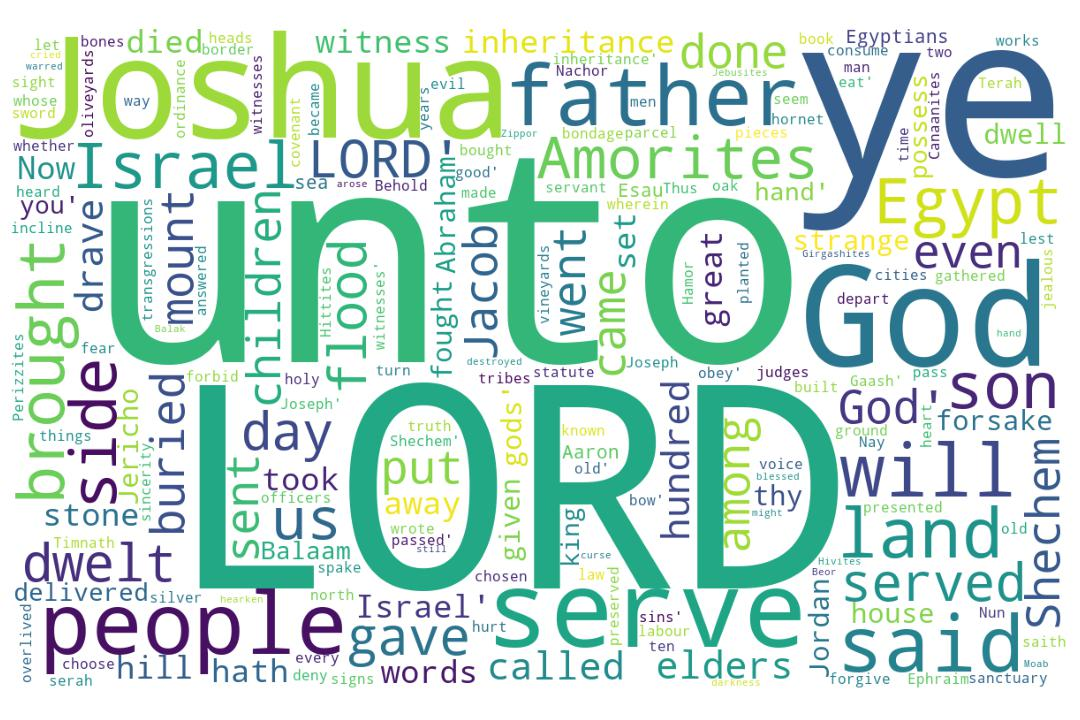
\includegraphics[width=\linewidth]{06OT-Joshua/Joshua24-WordCloud.jpg}
  \caption{Joshua 24 Word Cloud}
  \label{fig:Joshua 24 Word Cloud}
\end{figure}

\marginpar{\scriptsize \centering \fcolorbox{bone}{lime}{\textbf{JOSHUA'S SUMMARY}}\\ (Joshua 24)

\begin{compactenum}[I.][8]

	\item Story of a \textbf{Calling} \index[scripture]{Joshua!Jsh 24:03}(Jsh 24:3)
    \item Story of \textbf{Compassion} \index[scripture]{Joshua!Jsh 24:04}(Jsh 24:4)
    \item Story of \textbf{Covering} \index[scripture]{Joshua!Jsh 24:05}(Jsh 24:5)
    \item Story of \textbf{Conquering} \index[scripture]{Joshua!Jsh 24:08}(Jsh 24:8)
    \item Story of  \textbf{Commitment} \index[scripture]{Joshua!Jsh 24:14}(Jsh 24:14)
    \item Story of \textbf{Cleansing} \index[scripture]{Joshua!Jsh 24:23}(Jsh 24:23)
    \item Story of \textbf{Covenants} \index[scripture]{Joshua!Jsh 24:25}(Jsh 24:25)

\end{compactenum}}





\footnote{\textcolor[rgb]{0.00,0.25,0.00}{\hyperlink{TOC}{Return to end of Table of Contents.}}}\textcolor[cmyk]{0.99998,1,0,0}{And \fcolorbox{bone}{bone}{Joshua} gathered all the tribes of Israel to Shechem, and called for the elders of Israel, and for their heads, and for their judges, and for their officers; and they presented themselves before God.}
[2] \textcolor[cmyk]{0.99998,1,0,0}{And \fcolorbox{bone}{bone}{Joshua} said unto all the people, Thus saith the LORD God of Israel, Your fathers dwelt on the other side of the flood in old time, \emph{even} Terah, the father of Abraham, and the father of Nachor: and they served other gods.}
[3] \textcolor[cmyk]{0.99998,1,0,0}{And I took your father Abraham from the other side of the flood, and led him throughout all the land of Canaan, and multiplied his seed, and gave him Isaac.}\
[4] \textcolor[cmyk]{0.99998,1,0,0}{And I gave unto Isaac Jacob and Esau: and I gave unto Esau mount Seir, to possess it; but Jacob and his children went down into Egypt.}
[5] \textcolor[cmyk]{0.99998,1,0,0}{I sent Moses also and Aaron, and I plagued Egypt, according to that which I did among them: and afterward I brought you out.}
[6] \textcolor[cmyk]{0.99998,1,0,0}{And I brought your fathers out of Egypt: and ye came unto the sea; and the Egyptians pursued after your fathers with chariots and horsemen unto the Red sea.}
[7] \textcolor[cmyk]{0.99998,1,0,0}{And when they cried unto the LORD, he put darkness between you and the Egyptians, and brought the sea upon them, and covered them; and your eyes have seen what I have done in Egypt: and ye dwelt in the wilderness a long season.}
[8] \textcolor[cmyk]{0.99998,1,0,0}{And I brought you into the land of the Amorites, which dwelt on the other side Jordan; and they fought with you: and I gave them into your hand, that ye might possess their land; and I destroyed them from before you.}
[9] \textcolor[cmyk]{0.99998,1,0,0}{Then Balak the son of Zippor, king of Moab, arose and warred against Israel, and sent and called Balaam the son of Beor to curse you:}
[10] \textcolor[cmyk]{0.99998,1,0,0}{But I would not hearken unto Balaam; therefore he blessed you still: so I delivered you out of his hand.}
[11] \textcolor[cmyk]{0.99998,1,0,0}{And ye went over Jordan, and came unto Jericho: and the men of Jericho fought against you, the Amorites, and the Perizzites, and the Canaanites, and the Hittites, and the Girgashites, the Hivites, and the Jebusites; and I delivered them into your hand.}
[12] \textcolor[cmyk]{0.99998,1,0,0}{And I sent the hornet before you, which drave them out from before you, \emph{even} the two kings of the Amorites; \emph{but} not with thy sword, nor with thy bow.}
[13] \textcolor[cmyk]{0.99998,1,0,0}{And I have given you a land for which ye did not labour, and cities which ye built not, and ye dwell in them; of the vineyards and oliveyards which ye planted not do ye eat.}\\
\\
\P \textcolor[cmyk]{0.99998,1,0,0}{Now therefore fear the LORD, and serve him in sincerity and in truth: and put away the gods which your fathers served on the other side of the flood, and in Egypt; and serve ye the LORD.}
[15] \textcolor[cmyk]{0.99998,1,0,0}{And if it seem evil unto you to serve the LORD, choose you this day whom ye will serve; whether the gods which your fathers served that \emph{were} on the other side of the flood, or the gods of the Amorites, in whose land ye dwell: but as for me and my house, we will serve the LORD.}
[16] \textcolor[cmyk]{0.99998,1,0,0}{And the people answered and said, God forbid that we should forsake the LORD, to serve other gods;}
[17] \textcolor[cmyk]{0.99998,1,0,0}{For the LORD our God, he \emph{it} \emph{is} that brought us up and our fathers out of the land of Egypt, from the house of bondage, and which did those great signs in our sight, and preserved us in all the way wherein we went, and among all the people through whom we passed:}
[18] \textcolor[cmyk]{0.99998,1,0,0}{And the LORD drave out from before us all the people, even the Amorites which dwelt in the land: \emph{therefore} will we also serve the LORD; for he \emph{is} our God.}
[19] \textcolor[cmyk]{0.99998,1,0,0}{And \fcolorbox{bone}{bone}{Joshua} said unto the people, Ye cannot serve the LORD: for he \emph{is} an holy God; he \emph{is} a jealous God; he will not forgive your transgressions nor your sins.}
[20] \textcolor[cmyk]{0.99998,1,0,0}{If ye forsake the LORD, and serve strange gods, then he will turn and do you hurt, and consume you, after that he hath done you good.}
[21] \textcolor[cmyk]{0.99998,1,0,0}{And the people said unto \fcolorbox{bone}{bone}{Joshua}, Nay; but we will serve the LORD.}
[22] \textcolor[cmyk]{0.99998,1,0,0}{And \fcolorbox{bone}{bone}{Joshua} said unto the people, Ye \emph{are} witnesses against yourselves that ye have chosen you the LORD, to serve him. And they said, \emph{We} \emph{are} witnesses.}
[23] \textcolor[cmyk]{0.99998,1,0,0}{Now therefore put away, \emph{said} \emph{he}, the strange gods which \emph{are} among you, and incline your heart unto the LORD God of Israel.}
[24] \textcolor[cmyk]{0.99998,1,0,0}{And the people said unto \fcolorbox{bone}{bone}{Joshua}, The LORD our God will we serve, and his voice will we obey.}
[25] \textcolor[cmyk]{0.99998,1,0,0}{So \fcolorbox{bone}{bone}{Joshua} made a covenant with the people that day, and set them a statute and an ordinance in Shechem.}\\
\\
\P \textcolor[cmyk]{0.99998,1,0,0}{And \fcolorbox{bone}{bone}{Joshua} wrote these words in the book of the law of God, and took a great stone, and set it up there under an oak, that \emph{was} by the sanctuary of the LORD.}
[27] \textcolor[cmyk]{0.99998,1,0,0}{And \fcolorbox{bone}{bone}{Joshua} said unto all the people, Behold, this stone shall be a witness unto us; for it hath heard all the words of the LORD which he spake unto us: it shall be therefore a witness unto you, lest ye deny your God.}
[28] \textcolor[cmyk]{0.99998,1,0,0}{So \fcolorbox{bone}{bone}{Joshua} let the people depart, every man unto his inheritance.}\\
\\
\P \textcolor[cmyk]{0.99998,1,0,0}{And it came to pass after these things, that \fcolorbox{bone}{bone}{Joshua} the son of Nun, the servant of the LORD, died, \emph{being} an hundred and ten years old.}
[30] \textcolor[cmyk]{0.99998,1,0,0}{And they buried him in the border of his inheritance in Timnath-serah, which \emph{is} in mount Ephraim, on the north side of the hill of Gaash.}
[31] \textcolor[cmyk]{0.99998,1,0,0}{And Israel served the LORD all the days of \fcolorbox{bone}{bone}{Joshua}, and all the days of the elders that overlived \fcolorbox{bone}{bone}{Joshua}, and which had known all the works of the LORD, that he had done for Israel.}\\
\\
\P \textcolor[cmyk]{0.99998,1,0,0}{And the bones of Joseph, which the children of Israel brought up out of Egypt, buried they in Shechem, in a parcel of ground which Jacob bought of the sons of Hamor the father of Shechem for an hundred pieces of silver: and it became the inheritance of the children of Joseph.}
[33] \textcolor[cmyk]{0.99998,1,0,0}{And Eleazar the son of Aaron died; and they buried him in a hill \emph{that} \emph{pertained} \emph{to} Phinehas his son, which was given him in mount Ephraim.}


\index[NWIV]{35!Joshua!Jos 24:1}\index[AWIP]{And!Joshua!Jos 24:1}\index[AWIP]{Joshua!Joshua!Jos 24:1}\index[AWIP]{gathered!Joshua!Jos 24:1}\index[AWIP]{all!Joshua!Jos 24:1}\index[AWIP]{the!Joshua!Jos 24:1}\index[AWIP]{the!Joshua!Jos 24:1 (2)}\index[AWIP]{tribes!Joshua!Jos 24:1}\index[AWIP]{of!Joshua!Jos 24:1}\index[AWIP]{of!Joshua!Jos 24:1 (2)}\index[AWIP]{Israel!Joshua!Jos 24:1}\index[AWIP]{Israel!Joshua!Jos 24:1 (2)}\index[AWIP]{to!Joshua!Jos 24:1}\index[AWIP]{Shechem!Joshua!Jos 24:1}\index[AWIP]{and!Joshua!Jos 24:1}\index[AWIP]{and!Joshua!Jos 24:1 (2)}\index[AWIP]{and!Joshua!Jos 24:1 (3)}\index[AWIP]{and!Joshua!Jos 24:1 (4)}\index[AWIP]{and!Joshua!Jos 24:1 (5)}\index[AWIP]{called!Joshua!Jos 24:1}\index[AWIP]{for!Joshua!Jos 24:1}\index[AWIP]{for!Joshua!Jos 24:1 (2)}\index[AWIP]{for!Joshua!Jos 24:1 (3)}\index[AWIP]{for!Joshua!Jos 24:1 (4)}\index[AWIP]{elders!Joshua!Jos 24:1}\index[AWIP]{their!Joshua!Jos 24:1}\index[AWIP]{their!Joshua!Jos 24:1 (2)}\index[AWIP]{their!Joshua!Jos 24:1 (3)}\index[AWIP]{heads!Joshua!Jos 24:1}\index[AWIP]{judges!Joshua!Jos 24:1}\index[AWIP]{officers!Joshua!Jos 24:1}\index[AWIP]{they!Joshua!Jos 24:1}\index[AWIP]{presented!Joshua!Jos 24:1}\index[AWIP]{themselves!Joshua!Jos 24:1}\index[AWIP]{before!Joshua!Jos 24:1}\index[AWIP]{God!Joshua!Jos 24:1}

\index[NWIV]{43!Joshua!Jos 24:2}\index[AWIP]{And!Joshua!Jos 24:2}\index[AWIP]{Joshua!Joshua!Jos 24:2}\index[AWIP]{said!Joshua!Jos 24:2}\index[AWIP]{unto!Joshua!Jos 24:2}\index[AWIP]{all!Joshua!Jos 24:2}\index[AWIP]{the!Joshua!Jos 24:2}\index[AWIP]{the!Joshua!Jos 24:2 (2)}\index[AWIP]{the!Joshua!Jos 24:2 (3)}\index[AWIP]{the!Joshua!Jos 24:2 (4)}\index[AWIP]{the!Joshua!Jos 24:2 (5)}\index[AWIP]{the!Joshua!Jos 24:2 (6)}\index[AWIP]{people!Joshua!Jos 24:2}\index[AWIP]{Thus!Joshua!Jos 24:2}\index[AWIP]{saith!Joshua!Jos 24:2}\index[AWIP]{LORD!Joshua!Jos 24:2}\index[AWIP]{God!Joshua!Jos 24:2}\index[AWIP]{of!Joshua!Jos 24:2}\index[AWIP]{of!Joshua!Jos 24:2 (2)}\index[AWIP]{of!Joshua!Jos 24:2 (3)}\index[AWIP]{of!Joshua!Jos 24:2 (4)}\index[AWIP]{Israel!Joshua!Jos 24:2}\index[AWIP]{Your!Joshua!Jos 24:2}\index[AWIP]{fathers!Joshua!Jos 24:2}\index[AWIP]{dwelt!Joshua!Jos 24:2}\index[AWIP]{on!Joshua!Jos 24:2}\index[AWIP]{other!Joshua!Jos 24:2}\index[AWIP]{other!Joshua!Jos 24:2 (2)}\index[AWIP]{side!Joshua!Jos 24:2}\index[AWIP]{flood!Joshua!Jos 24:2}\index[AWIP]{in!Joshua!Jos 24:2}\index[AWIP]{old!Joshua!Jos 24:2}\index[AWIP]{time!Joshua!Jos 24:2}\index[AWIP]{\emph{even}!Joshua!Jos 24:2}\index[AWIP]{Terah!Joshua!Jos 24:2}\index[AWIP]{father!Joshua!Jos 24:2}\index[AWIP]{father!Joshua!Jos 24:2 (2)}\index[AWIP]{Abraham!Joshua!Jos 24:2}\index[AWIP]{and!Joshua!Jos 24:2}\index[AWIP]{and!Joshua!Jos 24:2 (2)}\index[AWIP]{Nachor!Joshua!Jos 24:2}\index[AWIP]{they!Joshua!Jos 24:2}\index[AWIP]{served!Joshua!Jos 24:2}\index[AWIP]{gods!Joshua!Jos 24:2}\index[AWIP]{\emph{even}!Joshua!Jos 24:2}

\index[NWIV]{30!Joshua!Jos 24:3}\index[AWIP]{And!Joshua!Jos 24:3}\index[AWIP]{I!Joshua!Jos 24:3}\index[AWIP]{took!Joshua!Jos 24:3}\index[AWIP]{your!Joshua!Jos 24:3}\index[AWIP]{father!Joshua!Jos 24:3}\index[AWIP]{Abraham!Joshua!Jos 24:3}\index[AWIP]{from!Joshua!Jos 24:3}\index[AWIP]{the!Joshua!Jos 24:3}\index[AWIP]{the!Joshua!Jos 24:3 (2)}\index[AWIP]{the!Joshua!Jos 24:3 (3)}\index[AWIP]{other!Joshua!Jos 24:3}\index[AWIP]{side!Joshua!Jos 24:3}\index[AWIP]{of!Joshua!Jos 24:3}\index[AWIP]{of!Joshua!Jos 24:3 (2)}\index[AWIP]{flood!Joshua!Jos 24:3}\index[AWIP]{and!Joshua!Jos 24:3}\index[AWIP]{and!Joshua!Jos 24:3 (2)}\index[AWIP]{and!Joshua!Jos 24:3 (3)}\index[AWIP]{led!Joshua!Jos 24:3}\index[AWIP]{him!Joshua!Jos 24:3}\index[AWIP]{him!Joshua!Jos 24:3 (2)}\index[AWIP]{throughout!Joshua!Jos 24:3}\index[AWIP]{all!Joshua!Jos 24:3}\index[AWIP]{land!Joshua!Jos 24:3}\index[AWIP]{Canaan!Joshua!Jos 24:3}\index[AWIP]{multiplied!Joshua!Jos 24:3}\index[AWIP]{his!Joshua!Jos 24:3}\index[AWIP]{seed!Joshua!Jos 24:3}\index[AWIP]{gave!Joshua!Jos 24:3}\index[AWIP]{Isaac!Joshua!Jos 24:3}

\index[NWIV]{27!Joshua!Jos 24:4}\index[AWIP]{And!Joshua!Jos 24:4}\index[AWIP]{I!Joshua!Jos 24:4}\index[AWIP]{I!Joshua!Jos 24:4 (2)}\index[AWIP]{gave!Joshua!Jos 24:4}\index[AWIP]{gave!Joshua!Jos 24:4 (2)}\index[AWIP]{unto!Joshua!Jos 24:4}\index[AWIP]{unto!Joshua!Jos 24:4 (2)}\index[AWIP]{Isaac!Joshua!Jos 24:4}\index[AWIP]{Jacob!Joshua!Jos 24:4}\index[AWIP]{Jacob!Joshua!Jos 24:4 (2)}\index[AWIP]{and!Joshua!Jos 24:4}\index[AWIP]{and!Joshua!Jos 24:4 (2)}\index[AWIP]{and!Joshua!Jos 24:4 (3)}\index[AWIP]{Esau!Joshua!Jos 24:4}\index[AWIP]{Esau!Joshua!Jos 24:4 (2)}\index[AWIP]{mount!Joshua!Jos 24:4}\index[AWIP]{Seir!Joshua!Jos 24:4}\index[AWIP]{to!Joshua!Jos 24:4}\index[AWIP]{possess!Joshua!Jos 24:4}\index[AWIP]{it!Joshua!Jos 24:4}\index[AWIP]{but!Joshua!Jos 24:4}\index[AWIP]{his!Joshua!Jos 24:4}\index[AWIP]{children!Joshua!Jos 24:4}\index[AWIP]{went!Joshua!Jos 24:4}\index[AWIP]{down!Joshua!Jos 24:4}\index[AWIP]{into!Joshua!Jos 24:4}\index[AWIP]{Egypt!Joshua!Jos 24:4}

\index[NWIV]{24!Joshua!Jos 24:5}\index[AWIP]{I!Joshua!Jos 24:5}\index[AWIP]{I!Joshua!Jos 24:5 (2)}\index[AWIP]{I!Joshua!Jos 24:5 (3)}\index[AWIP]{I!Joshua!Jos 24:5 (4)}\index[AWIP]{sent!Joshua!Jos 24:5}\index[AWIP]{Moses!Joshua!Jos 24:5}\index[AWIP]{also!Joshua!Jos 24:5}\index[AWIP]{and!Joshua!Jos 24:5}\index[AWIP]{and!Joshua!Jos 24:5 (2)}\index[AWIP]{and!Joshua!Jos 24:5 (3)}\index[AWIP]{Aaron!Joshua!Jos 24:5}\index[AWIP]{plagued!Joshua!Jos 24:5}\index[AWIP]{Egypt!Joshua!Jos 24:5}\index[AWIP]{according!Joshua!Jos 24:5}\index[AWIP]{to!Joshua!Jos 24:5}\index[AWIP]{that!Joshua!Jos 24:5}\index[AWIP]{which!Joshua!Jos 24:5}\index[AWIP]{did!Joshua!Jos 24:5}\index[AWIP]{among!Joshua!Jos 24:5}\index[AWIP]{them!Joshua!Jos 24:5}\index[AWIP]{afterward!Joshua!Jos 24:5}\index[AWIP]{brought!Joshua!Jos 24:5}\index[AWIP]{you!Joshua!Jos 24:5}\index[AWIP]{out!Joshua!Jos 24:5}

\index[NWIV]{29!Joshua!Jos 24:6}\index[AWIP]{And!Joshua!Jos 24:6}\index[AWIP]{I!Joshua!Jos 24:6}\index[AWIP]{brought!Joshua!Jos 24:6}\index[AWIP]{your!Joshua!Jos 24:6}\index[AWIP]{your!Joshua!Jos 24:6 (2)}\index[AWIP]{fathers!Joshua!Jos 24:6}\index[AWIP]{fathers!Joshua!Jos 24:6 (2)}\index[AWIP]{out!Joshua!Jos 24:6}\index[AWIP]{of!Joshua!Jos 24:6}\index[AWIP]{Egypt!Joshua!Jos 24:6}\index[AWIP]{and!Joshua!Jos 24:6}\index[AWIP]{and!Joshua!Jos 24:6 (2)}\index[AWIP]{and!Joshua!Jos 24:6 (3)}\index[AWIP]{ye!Joshua!Jos 24:6}\index[AWIP]{came!Joshua!Jos 24:6}\index[AWIP]{unto!Joshua!Jos 24:6}\index[AWIP]{unto!Joshua!Jos 24:6 (2)}\index[AWIP]{the!Joshua!Jos 24:6}\index[AWIP]{the!Joshua!Jos 24:6 (2)}\index[AWIP]{the!Joshua!Jos 24:6 (3)}\index[AWIP]{sea!Joshua!Jos 24:6}\index[AWIP]{sea!Joshua!Jos 24:6 (2)}\index[AWIP]{Egyptians!Joshua!Jos 24:6}\index[AWIP]{pursued!Joshua!Jos 24:6}\index[AWIP]{after!Joshua!Jos 24:6}\index[AWIP]{with!Joshua!Jos 24:6}\index[AWIP]{chariots!Joshua!Jos 24:6}\index[AWIP]{horsemen!Joshua!Jos 24:6}\index[AWIP]{Red!Joshua!Jos 24:6}

\index[NWIV]{44!Joshua!Jos 24:7}\index[AWIP]{And!Joshua!Jos 24:7}\index[AWIP]{when!Joshua!Jos 24:7}\index[AWIP]{they!Joshua!Jos 24:7}\index[AWIP]{cried!Joshua!Jos 24:7}\index[AWIP]{unto!Joshua!Jos 24:7}\index[AWIP]{the!Joshua!Jos 24:7}\index[AWIP]{the!Joshua!Jos 24:7 (2)}\index[AWIP]{the!Joshua!Jos 24:7 (3)}\index[AWIP]{the!Joshua!Jos 24:7 (4)}\index[AWIP]{LORD!Joshua!Jos 24:7}\index[AWIP]{he!Joshua!Jos 24:7}\index[AWIP]{put!Joshua!Jos 24:7}\index[AWIP]{darkness!Joshua!Jos 24:7}\index[AWIP]{between!Joshua!Jos 24:7}\index[AWIP]{you!Joshua!Jos 24:7}\index[AWIP]{and!Joshua!Jos 24:7}\index[AWIP]{and!Joshua!Jos 24:7 (2)}\index[AWIP]{and!Joshua!Jos 24:7 (3)}\index[AWIP]{and!Joshua!Jos 24:7 (4)}\index[AWIP]{and!Joshua!Jos 24:7 (5)}\index[AWIP]{Egyptians!Joshua!Jos 24:7}\index[AWIP]{brought!Joshua!Jos 24:7}\index[AWIP]{sea!Joshua!Jos 24:7}\index[AWIP]{upon!Joshua!Jos 24:7}\index[AWIP]{them!Joshua!Jos 24:7}\index[AWIP]{them!Joshua!Jos 24:7 (2)}\index[AWIP]{covered!Joshua!Jos 24:7}\index[AWIP]{your!Joshua!Jos 24:7}\index[AWIP]{eyes!Joshua!Jos 24:7}\index[AWIP]{have!Joshua!Jos 24:7}\index[AWIP]{have!Joshua!Jos 24:7 (2)}\index[AWIP]{seen!Joshua!Jos 24:7}\index[AWIP]{what!Joshua!Jos 24:7}\index[AWIP]{I!Joshua!Jos 24:7}\index[AWIP]{done!Joshua!Jos 24:7}\index[AWIP]{in!Joshua!Jos 24:7}\index[AWIP]{in!Joshua!Jos 24:7 (2)}\index[AWIP]{Egypt!Joshua!Jos 24:7}\index[AWIP]{ye!Joshua!Jos 24:7}\index[AWIP]{dwelt!Joshua!Jos 24:7}\index[AWIP]{wilderness!Joshua!Jos 24:7}\index[AWIP]{a!Joshua!Jos 24:7}\index[AWIP]{long!Joshua!Jos 24:7}\index[AWIP]{season!Joshua!Jos 24:7}

\index[NWIV]{42!Joshua!Jos 24:8}\index[AWIP]{And!Joshua!Jos 24:8}\index[AWIP]{I!Joshua!Jos 24:8}\index[AWIP]{I!Joshua!Jos 24:8 (2)}\index[AWIP]{I!Joshua!Jos 24:8 (3)}\index[AWIP]{brought!Joshua!Jos 24:8}\index[AWIP]{you!Joshua!Jos 24:8}\index[AWIP]{you!Joshua!Jos 24:8 (2)}\index[AWIP]{you!Joshua!Jos 24:8 (3)}\index[AWIP]{into!Joshua!Jos 24:8}\index[AWIP]{into!Joshua!Jos 24:8 (2)}\index[AWIP]{the!Joshua!Jos 24:8}\index[AWIP]{the!Joshua!Jos 24:8 (2)}\index[AWIP]{the!Joshua!Jos 24:8 (3)}\index[AWIP]{land!Joshua!Jos 24:8}\index[AWIP]{land!Joshua!Jos 24:8 (2)}\index[AWIP]{of!Joshua!Jos 24:8}\index[AWIP]{Amorites!Joshua!Jos 24:8}\index[AWIP]{which!Joshua!Jos 24:8}\index[AWIP]{dwelt!Joshua!Jos 24:8}\index[AWIP]{on!Joshua!Jos 24:8}\index[AWIP]{other!Joshua!Jos 24:8}\index[AWIP]{side!Joshua!Jos 24:8}\index[AWIP]{Jordan!Joshua!Jos 24:8}\index[AWIP]{and!Joshua!Jos 24:8}\index[AWIP]{and!Joshua!Jos 24:8 (2)}\index[AWIP]{and!Joshua!Jos 24:8 (3)}\index[AWIP]{they!Joshua!Jos 24:8}\index[AWIP]{fought!Joshua!Jos 24:8}\index[AWIP]{with!Joshua!Jos 24:8}\index[AWIP]{gave!Joshua!Jos 24:8}\index[AWIP]{them!Joshua!Jos 24:8}\index[AWIP]{them!Joshua!Jos 24:8 (2)}\index[AWIP]{your!Joshua!Jos 24:8}\index[AWIP]{hand!Joshua!Jos 24:8}\index[AWIP]{that!Joshua!Jos 24:8}\index[AWIP]{ye!Joshua!Jos 24:8}\index[AWIP]{might!Joshua!Jos 24:8}\index[AWIP]{possess!Joshua!Jos 24:8}\index[AWIP]{their!Joshua!Jos 24:8}\index[AWIP]{destroyed!Joshua!Jos 24:8}\index[AWIP]{from!Joshua!Jos 24:8}\index[AWIP]{before!Joshua!Jos 24:8}

\index[NWIV]{26!Joshua!Jos 24:9}\index[AWIP]{Then!Joshua!Jos 24:9}\index[AWIP]{Balak!Joshua!Jos 24:9}\index[AWIP]{the!Joshua!Jos 24:9}\index[AWIP]{the!Joshua!Jos 24:9 (2)}\index[AWIP]{son!Joshua!Jos 24:9}\index[AWIP]{son!Joshua!Jos 24:9 (2)}\index[AWIP]{of!Joshua!Jos 24:9}\index[AWIP]{of!Joshua!Jos 24:9 (2)}\index[AWIP]{of!Joshua!Jos 24:9 (3)}\index[AWIP]{Zippor!Joshua!Jos 24:9}\index[AWIP]{king!Joshua!Jos 24:9}\index[AWIP]{Moab!Joshua!Jos 24:9}\index[AWIP]{arose!Joshua!Jos 24:9}\index[AWIP]{and!Joshua!Jos 24:9}\index[AWIP]{and!Joshua!Jos 24:9 (2)}\index[AWIP]{and!Joshua!Jos 24:9 (3)}\index[AWIP]{warred!Joshua!Jos 24:9}\index[AWIP]{against!Joshua!Jos 24:9}\index[AWIP]{Israel!Joshua!Jos 24:9}\index[AWIP]{sent!Joshua!Jos 24:9}\index[AWIP]{called!Joshua!Jos 24:9}\index[AWIP]{Balaam!Joshua!Jos 24:9}\index[AWIP]{Beor!Joshua!Jos 24:9}\index[AWIP]{to!Joshua!Jos 24:9}\index[AWIP]{curse!Joshua!Jos 24:9}\index[AWIP]{you!Joshua!Jos 24:9}

\index[NWIV]{20!Joshua!Jos 24:10}\index[AWIP]{But!Joshua!Jos 24:10}\index[AWIP]{I!Joshua!Jos 24:10}\index[AWIP]{I!Joshua!Jos 24:10 (2)}\index[AWIP]{would!Joshua!Jos 24:10}\index[AWIP]{not!Joshua!Jos 24:10}\index[AWIP]{hearken!Joshua!Jos 24:10}\index[AWIP]{unto!Joshua!Jos 24:10}\index[AWIP]{Balaam!Joshua!Jos 24:10}\index[AWIP]{therefore!Joshua!Jos 24:10}\index[AWIP]{he!Joshua!Jos 24:10}\index[AWIP]{blessed!Joshua!Jos 24:10}\index[AWIP]{you!Joshua!Jos 24:10}\index[AWIP]{you!Joshua!Jos 24:10 (2)}\index[AWIP]{still!Joshua!Jos 24:10}\index[AWIP]{so!Joshua!Jos 24:10}\index[AWIP]{delivered!Joshua!Jos 24:10}\index[AWIP]{out!Joshua!Jos 24:10}\index[AWIP]{of!Joshua!Jos 24:10}\index[AWIP]{his!Joshua!Jos 24:10}\index[AWIP]{hand!Joshua!Jos 24:10}

\index[NWIV]{43!Joshua!Jos 24:11}\index[AWIP]{And!Joshua!Jos 24:11}\index[AWIP]{ye!Joshua!Jos 24:11}\index[AWIP]{went!Joshua!Jos 24:11}\index[AWIP]{over!Joshua!Jos 24:11}\index[AWIP]{Jordan!Joshua!Jos 24:11}\index[AWIP]{and!Joshua!Jos 24:11}\index[AWIP]{and!Joshua!Jos 24:11 (2)}\index[AWIP]{and!Joshua!Jos 24:11 (3)}\index[AWIP]{and!Joshua!Jos 24:11 (4)}\index[AWIP]{and!Joshua!Jos 24:11 (5)}\index[AWIP]{and!Joshua!Jos 24:11 (6)}\index[AWIP]{and!Joshua!Jos 24:11 (7)}\index[AWIP]{and!Joshua!Jos 24:11 (8)}\index[AWIP]{came!Joshua!Jos 24:11}\index[AWIP]{unto!Joshua!Jos 24:11}\index[AWIP]{Jericho!Joshua!Jos 24:11}\index[AWIP]{Jericho!Joshua!Jos 24:11 (2)}\index[AWIP]{the!Joshua!Jos 24:11}\index[AWIP]{the!Joshua!Jos 24:11 (2)}\index[AWIP]{the!Joshua!Jos 24:11 (3)}\index[AWIP]{the!Joshua!Jos 24:11 (4)}\index[AWIP]{the!Joshua!Jos 24:11 (5)}\index[AWIP]{the!Joshua!Jos 24:11 (6)}\index[AWIP]{the!Joshua!Jos 24:11 (7)}\index[AWIP]{the!Joshua!Jos 24:11 (8)}\index[AWIP]{men!Joshua!Jos 24:11}\index[AWIP]{of!Joshua!Jos 24:11}\index[AWIP]{fought!Joshua!Jos 24:11}\index[AWIP]{against!Joshua!Jos 24:11}\index[AWIP]{you!Joshua!Jos 24:11}\index[AWIP]{Amorites!Joshua!Jos 24:11}\index[AWIP]{Perizzites!Joshua!Jos 24:11}\index[AWIP]{Canaanites!Joshua!Jos 24:11}\index[AWIP]{Hittites!Joshua!Jos 24:11}\index[AWIP]{Girgashites!Joshua!Jos 24:11}\index[AWIP]{Hivites!Joshua!Jos 24:11}\index[AWIP]{Jebusites!Joshua!Jos 24:11}\index[AWIP]{I!Joshua!Jos 24:11}\index[AWIP]{delivered!Joshua!Jos 24:11}\index[AWIP]{them!Joshua!Jos 24:11}\index[AWIP]{into!Joshua!Jos 24:11}\index[AWIP]{your!Joshua!Jos 24:11}\index[AWIP]{hand!Joshua!Jos 24:11}

\index[NWIV]{30!Joshua!Jos 24:12}\index[AWIP]{And!Joshua!Jos 24:12}\index[AWIP]{I!Joshua!Jos 24:12}\index[AWIP]{sent!Joshua!Jos 24:12}\index[AWIP]{the!Joshua!Jos 24:12}\index[AWIP]{the!Joshua!Jos 24:12 (2)}\index[AWIP]{the!Joshua!Jos 24:12 (3)}\index[AWIP]{hornet!Joshua!Jos 24:12}\index[AWIP]{before!Joshua!Jos 24:12}\index[AWIP]{before!Joshua!Jos 24:12 (2)}\index[AWIP]{you!Joshua!Jos 24:12}\index[AWIP]{you!Joshua!Jos 24:12 (2)}\index[AWIP]{which!Joshua!Jos 24:12}\index[AWIP]{drave!Joshua!Jos 24:12}\index[AWIP]{them!Joshua!Jos 24:12}\index[AWIP]{out!Joshua!Jos 24:12}\index[AWIP]{from!Joshua!Jos 24:12}\index[AWIP]{\emph{even}!Joshua!Jos 24:12}\index[AWIP]{two!Joshua!Jos 24:12}\index[AWIP]{kings!Joshua!Jos 24:12}\index[AWIP]{of!Joshua!Jos 24:12}\index[AWIP]{Amorites!Joshua!Jos 24:12}\index[AWIP]{\emph{but}!Joshua!Jos 24:12}\index[AWIP]{not!Joshua!Jos 24:12}\index[AWIP]{with!Joshua!Jos 24:12}\index[AWIP]{with!Joshua!Jos 24:12 (2)}\index[AWIP]{thy!Joshua!Jos 24:12}\index[AWIP]{thy!Joshua!Jos 24:12 (2)}\index[AWIP]{sword!Joshua!Jos 24:12}\index[AWIP]{nor!Joshua!Jos 24:12}\index[AWIP]{bow!Joshua!Jos 24:12}\index[AWIP]{\emph{even}!Joshua!Jos 24:12}\index[AWIP]{\emph{but}!Joshua!Jos 24:12}

\index[NWIV]{36!Joshua!Jos 24:13}\index[AWIP]{And!Joshua!Jos 24:13}\index[AWIP]{I!Joshua!Jos 24:13}\index[AWIP]{have!Joshua!Jos 24:13}\index[AWIP]{given!Joshua!Jos 24:13}\index[AWIP]{you!Joshua!Jos 24:13}\index[AWIP]{a!Joshua!Jos 24:13}\index[AWIP]{land!Joshua!Jos 24:13}\index[AWIP]{for!Joshua!Jos 24:13}\index[AWIP]{which!Joshua!Jos 24:13}\index[AWIP]{which!Joshua!Jos 24:13 (2)}\index[AWIP]{which!Joshua!Jos 24:13 (3)}\index[AWIP]{ye!Joshua!Jos 24:13}\index[AWIP]{ye!Joshua!Jos 24:13 (2)}\index[AWIP]{ye!Joshua!Jos 24:13 (3)}\index[AWIP]{ye!Joshua!Jos 24:13 (4)}\index[AWIP]{ye!Joshua!Jos 24:13 (5)}\index[AWIP]{did!Joshua!Jos 24:13}\index[AWIP]{not!Joshua!Jos 24:13}\index[AWIP]{not!Joshua!Jos 24:13 (2)}\index[AWIP]{not!Joshua!Jos 24:13 (3)}\index[AWIP]{labour!Joshua!Jos 24:13}\index[AWIP]{and!Joshua!Jos 24:13}\index[AWIP]{and!Joshua!Jos 24:13 (2)}\index[AWIP]{and!Joshua!Jos 24:13 (3)}\index[AWIP]{cities!Joshua!Jos 24:13}\index[AWIP]{built!Joshua!Jos 24:13}\index[AWIP]{dwell!Joshua!Jos 24:13}\index[AWIP]{in!Joshua!Jos 24:13}\index[AWIP]{them!Joshua!Jos 24:13}\index[AWIP]{of!Joshua!Jos 24:13}\index[AWIP]{the!Joshua!Jos 24:13}\index[AWIP]{vineyards!Joshua!Jos 24:13}\index[AWIP]{oliveyards!Joshua!Jos 24:13}\index[AWIP]{planted!Joshua!Jos 24:13}\index[AWIP]{do!Joshua!Jos 24:13}\index[AWIP]{eat!Joshua!Jos 24:13}

\index[NWIV]{37!Joshua!Jos 24:14}\index[AWIP]{Now!Joshua!Jos 24:14}\index[AWIP]{therefore!Joshua!Jos 24:14}\index[AWIP]{fear!Joshua!Jos 24:14}\index[AWIP]{the!Joshua!Jos 24:14}\index[AWIP]{the!Joshua!Jos 24:14 (2)}\index[AWIP]{the!Joshua!Jos 24:14 (3)}\index[AWIP]{the!Joshua!Jos 24:14 (4)}\index[AWIP]{the!Joshua!Jos 24:14 (5)}\index[AWIP]{LORD!Joshua!Jos 24:14}\index[AWIP]{LORD!Joshua!Jos 24:14 (2)}\index[AWIP]{and!Joshua!Jos 24:14}\index[AWIP]{and!Joshua!Jos 24:14 (2)}\index[AWIP]{and!Joshua!Jos 24:14 (3)}\index[AWIP]{and!Joshua!Jos 24:14 (4)}\index[AWIP]{and!Joshua!Jos 24:14 (5)}\index[AWIP]{serve!Joshua!Jos 24:14}\index[AWIP]{serve!Joshua!Jos 24:14 (2)}\index[AWIP]{him!Joshua!Jos 24:14}\index[AWIP]{in!Joshua!Jos 24:14}\index[AWIP]{in!Joshua!Jos 24:14 (2)}\index[AWIP]{in!Joshua!Jos 24:14 (3)}\index[AWIP]{sincerity!Joshua!Jos 24:14}\index[AWIP]{truth!Joshua!Jos 24:14}\index[AWIP]{put!Joshua!Jos 24:14}\index[AWIP]{away!Joshua!Jos 24:14}\index[AWIP]{gods!Joshua!Jos 24:14}\index[AWIP]{which!Joshua!Jos 24:14}\index[AWIP]{your!Joshua!Jos 24:14}\index[AWIP]{fathers!Joshua!Jos 24:14}\index[AWIP]{served!Joshua!Jos 24:14}\index[AWIP]{on!Joshua!Jos 24:14}\index[AWIP]{other!Joshua!Jos 24:14}\index[AWIP]{side!Joshua!Jos 24:14}\index[AWIP]{of!Joshua!Jos 24:14}\index[AWIP]{flood!Joshua!Jos 24:14}\index[AWIP]{Egypt!Joshua!Jos 24:14}\index[AWIP]{ye!Joshua!Jos 24:14}

\index[NWIV]{58!Joshua!Jos 24:15}\index[AWIP]{And!Joshua!Jos 24:15}\index[AWIP]{if!Joshua!Jos 24:15}\index[AWIP]{it!Joshua!Jos 24:15}\index[AWIP]{seem!Joshua!Jos 24:15}\index[AWIP]{evil!Joshua!Jos 24:15}\index[AWIP]{unto!Joshua!Jos 24:15}\index[AWIP]{you!Joshua!Jos 24:15}\index[AWIP]{you!Joshua!Jos 24:15 (2)}\index[AWIP]{to!Joshua!Jos 24:15}\index[AWIP]{serve!Joshua!Jos 24:15}\index[AWIP]{serve!Joshua!Jos 24:15 (2)}\index[AWIP]{serve!Joshua!Jos 24:15 (3)}\index[AWIP]{the!Joshua!Jos 24:15}\index[AWIP]{the!Joshua!Jos 24:15 (2)}\index[AWIP]{the!Joshua!Jos 24:15 (3)}\index[AWIP]{the!Joshua!Jos 24:15 (4)}\index[AWIP]{the!Joshua!Jos 24:15 (5)}\index[AWIP]{the!Joshua!Jos 24:15 (6)}\index[AWIP]{the!Joshua!Jos 24:15 (7)}\index[AWIP]{LORD!Joshua!Jos 24:15}\index[AWIP]{LORD!Joshua!Jos 24:15 (2)}\index[AWIP]{choose!Joshua!Jos 24:15}\index[AWIP]{this!Joshua!Jos 24:15}\index[AWIP]{day!Joshua!Jos 24:15}\index[AWIP]{whom!Joshua!Jos 24:15}\index[AWIP]{ye!Joshua!Jos 24:15}\index[AWIP]{ye!Joshua!Jos 24:15 (2)}\index[AWIP]{will!Joshua!Jos 24:15}\index[AWIP]{will!Joshua!Jos 24:15 (2)}\index[AWIP]{whether!Joshua!Jos 24:15}\index[AWIP]{gods!Joshua!Jos 24:15}\index[AWIP]{gods!Joshua!Jos 24:15 (2)}\index[AWIP]{which!Joshua!Jos 24:15}\index[AWIP]{your!Joshua!Jos 24:15}\index[AWIP]{fathers!Joshua!Jos 24:15}\index[AWIP]{served!Joshua!Jos 24:15}\index[AWIP]{that!Joshua!Jos 24:15}\index[AWIP]{\emph{were}!Joshua!Jos 24:15}\index[AWIP]{on!Joshua!Jos 24:15}\index[AWIP]{other!Joshua!Jos 24:15}\index[AWIP]{side!Joshua!Jos 24:15}\index[AWIP]{of!Joshua!Jos 24:15}\index[AWIP]{of!Joshua!Jos 24:15 (2)}\index[AWIP]{flood!Joshua!Jos 24:15}\index[AWIP]{or!Joshua!Jos 24:15}\index[AWIP]{Amorites!Joshua!Jos 24:15}\index[AWIP]{in!Joshua!Jos 24:15}\index[AWIP]{whose!Joshua!Jos 24:15}\index[AWIP]{land!Joshua!Jos 24:15}\index[AWIP]{dwell!Joshua!Jos 24:15}\index[AWIP]{but!Joshua!Jos 24:15}\index[AWIP]{as!Joshua!Jos 24:15}\index[AWIP]{for!Joshua!Jos 24:15}\index[AWIP]{me!Joshua!Jos 24:15}\index[AWIP]{and!Joshua!Jos 24:15}\index[AWIP]{my!Joshua!Jos 24:15}\index[AWIP]{house!Joshua!Jos 24:15}\index[AWIP]{we!Joshua!Jos 24:15}\index[AWIP]{\emph{were}!Joshua!Jos 24:15}

\index[NWIV]{18!Joshua!Jos 24:16}\index[AWIP]{And!Joshua!Jos 24:16}\index[AWIP]{the!Joshua!Jos 24:16}\index[AWIP]{the!Joshua!Jos 24:16 (2)}\index[AWIP]{people!Joshua!Jos 24:16}\index[AWIP]{answered!Joshua!Jos 24:16}\index[AWIP]{and!Joshua!Jos 24:16}\index[AWIP]{said!Joshua!Jos 24:16}\index[AWIP]{God!Joshua!Jos 24:16}\index[AWIP]{forbid!Joshua!Jos 24:16}\index[AWIP]{that!Joshua!Jos 24:16}\index[AWIP]{we!Joshua!Jos 24:16}\index[AWIP]{should!Joshua!Jos 24:16}\index[AWIP]{forsake!Joshua!Jos 24:16}\index[AWIP]{LORD!Joshua!Jos 24:16}\index[AWIP]{to!Joshua!Jos 24:16}\index[AWIP]{serve!Joshua!Jos 24:16}\index[AWIP]{other!Joshua!Jos 24:16}\index[AWIP]{gods!Joshua!Jos 24:16}

\index[NWIV]{54!Joshua!Jos 24:17}\index[AWIP]{For!Joshua!Jos 24:17}\index[AWIP]{the!Joshua!Jos 24:17}\index[AWIP]{the!Joshua!Jos 24:17 (2)}\index[AWIP]{the!Joshua!Jos 24:17 (3)}\index[AWIP]{the!Joshua!Jos 24:17 (4)}\index[AWIP]{the!Joshua!Jos 24:17 (5)}\index[AWIP]{LORD!Joshua!Jos 24:17}\index[AWIP]{our!Joshua!Jos 24:17}\index[AWIP]{our!Joshua!Jos 24:17 (2)}\index[AWIP]{our!Joshua!Jos 24:17 (3)}\index[AWIP]{God!Joshua!Jos 24:17}\index[AWIP]{he!Joshua!Jos 24:17}\index[AWIP]{\emph{it}!Joshua!Jos 24:17}\index[AWIP]{\emph{is}!Joshua!Jos 24:17}\index[AWIP]{that!Joshua!Jos 24:17}\index[AWIP]{brought!Joshua!Jos 24:17}\index[AWIP]{us!Joshua!Jos 24:17}\index[AWIP]{us!Joshua!Jos 24:17 (2)}\index[AWIP]{up!Joshua!Jos 24:17}\index[AWIP]{and!Joshua!Jos 24:17}\index[AWIP]{and!Joshua!Jos 24:17 (2)}\index[AWIP]{and!Joshua!Jos 24:17 (3)}\index[AWIP]{and!Joshua!Jos 24:17 (4)}\index[AWIP]{fathers!Joshua!Jos 24:17}\index[AWIP]{out!Joshua!Jos 24:17}\index[AWIP]{of!Joshua!Jos 24:17}\index[AWIP]{of!Joshua!Jos 24:17 (2)}\index[AWIP]{of!Joshua!Jos 24:17 (3)}\index[AWIP]{land!Joshua!Jos 24:17}\index[AWIP]{Egypt!Joshua!Jos 24:17}\index[AWIP]{from!Joshua!Jos 24:17}\index[AWIP]{house!Joshua!Jos 24:17}\index[AWIP]{bondage!Joshua!Jos 24:17}\index[AWIP]{which!Joshua!Jos 24:17}\index[AWIP]{did!Joshua!Jos 24:17}\index[AWIP]{those!Joshua!Jos 24:17}\index[AWIP]{great!Joshua!Jos 24:17}\index[AWIP]{signs!Joshua!Jos 24:17}\index[AWIP]{in!Joshua!Jos 24:17}\index[AWIP]{in!Joshua!Jos 24:17 (2)}\index[AWIP]{sight!Joshua!Jos 24:17}\index[AWIP]{preserved!Joshua!Jos 24:17}\index[AWIP]{all!Joshua!Jos 24:17}\index[AWIP]{all!Joshua!Jos 24:17 (2)}\index[AWIP]{way!Joshua!Jos 24:17}\index[AWIP]{wherein!Joshua!Jos 24:17}\index[AWIP]{we!Joshua!Jos 24:17}\index[AWIP]{we!Joshua!Jos 24:17 (2)}\index[AWIP]{went!Joshua!Jos 24:17}\index[AWIP]{among!Joshua!Jos 24:17}\index[AWIP]{people!Joshua!Jos 24:17}\index[AWIP]{through!Joshua!Jos 24:17}\index[AWIP]{whom!Joshua!Jos 24:17}\index[AWIP]{passed!Joshua!Jos 24:17}\index[AWIP]{\emph{it}!Joshua!Jos 24:17}\index[AWIP]{\emph{is}!Joshua!Jos 24:17}

\index[NWIV]{31!Joshua!Jos 24:18}\index[AWIP]{And!Joshua!Jos 24:18}\index[AWIP]{the!Joshua!Jos 24:18}\index[AWIP]{the!Joshua!Jos 24:18 (2)}\index[AWIP]{the!Joshua!Jos 24:18 (3)}\index[AWIP]{the!Joshua!Jos 24:18 (4)}\index[AWIP]{the!Joshua!Jos 24:18 (5)}\index[AWIP]{LORD!Joshua!Jos 24:18}\index[AWIP]{LORD!Joshua!Jos 24:18 (2)}\index[AWIP]{drave!Joshua!Jos 24:18}\index[AWIP]{out!Joshua!Jos 24:18}\index[AWIP]{from!Joshua!Jos 24:18}\index[AWIP]{before!Joshua!Jos 24:18}\index[AWIP]{us!Joshua!Jos 24:18}\index[AWIP]{all!Joshua!Jos 24:18}\index[AWIP]{people!Joshua!Jos 24:18}\index[AWIP]{even!Joshua!Jos 24:18}\index[AWIP]{Amorites!Joshua!Jos 24:18}\index[AWIP]{which!Joshua!Jos 24:18}\index[AWIP]{dwelt!Joshua!Jos 24:18}\index[AWIP]{in!Joshua!Jos 24:18}\index[AWIP]{land!Joshua!Jos 24:18}\index[AWIP]{\emph{therefore}!Joshua!Jos 24:18}\index[AWIP]{will!Joshua!Jos 24:18}\index[AWIP]{we!Joshua!Jos 24:18}\index[AWIP]{also!Joshua!Jos 24:18}\index[AWIP]{serve!Joshua!Jos 24:18}\index[AWIP]{for!Joshua!Jos 24:18}\index[AWIP]{he!Joshua!Jos 24:18}\index[AWIP]{\emph{is}!Joshua!Jos 24:18}\index[AWIP]{our!Joshua!Jos 24:18}\index[AWIP]{God!Joshua!Jos 24:18}\index[AWIP]{\emph{therefore}!Joshua!Jos 24:18}\index[AWIP]{\emph{is}!Joshua!Jos 24:18}

\index[NWIV]{31!Joshua!Jos 24:19}\index[AWIP]{And!Joshua!Jos 24:19}\index[AWIP]{Joshua!Joshua!Jos 24:19}\index[AWIP]{said!Joshua!Jos 24:19}\index[AWIP]{unto!Joshua!Jos 24:19}\index[AWIP]{the!Joshua!Jos 24:19}\index[AWIP]{the!Joshua!Jos 24:19 (2)}\index[AWIP]{people!Joshua!Jos 24:19}\index[AWIP]{Ye!Joshua!Jos 24:19}\index[AWIP]{cannot!Joshua!Jos 24:19}\index[AWIP]{serve!Joshua!Jos 24:19}\index[AWIP]{LORD!Joshua!Jos 24:19}\index[AWIP]{for!Joshua!Jos 24:19}\index[AWIP]{he!Joshua!Jos 24:19}\index[AWIP]{he!Joshua!Jos 24:19 (2)}\index[AWIP]{he!Joshua!Jos 24:19 (3)}\index[AWIP]{\emph{is}!Joshua!Jos 24:19}\index[AWIP]{\emph{is}!Joshua!Jos 24:19 (2)}\index[AWIP]{an!Joshua!Jos 24:19}\index[AWIP]{holy!Joshua!Jos 24:19}\index[AWIP]{God!Joshua!Jos 24:19}\index[AWIP]{God!Joshua!Jos 24:19 (2)}\index[AWIP]{a!Joshua!Jos 24:19}\index[AWIP]{jealous!Joshua!Jos 24:19}\index[AWIP]{will!Joshua!Jos 24:19}\index[AWIP]{not!Joshua!Jos 24:19}\index[AWIP]{forgive!Joshua!Jos 24:19}\index[AWIP]{your!Joshua!Jos 24:19}\index[AWIP]{your!Joshua!Jos 24:19 (2)}\index[AWIP]{transgressions!Joshua!Jos 24:19}\index[AWIP]{nor!Joshua!Jos 24:19}\index[AWIP]{sins!Joshua!Jos 24:19}\index[AWIP]{\emph{is}!Joshua!Jos 24:19}\index[AWIP]{\emph{is}!Joshua!Jos 24:19 (2)}

\index[NWIV]{27!Joshua!Jos 24:20}\index[AWIP]{If!Joshua!Jos 24:20}\index[AWIP]{ye!Joshua!Jos 24:20}\index[AWIP]{forsake!Joshua!Jos 24:20}\index[AWIP]{the!Joshua!Jos 24:20}\index[AWIP]{LORD!Joshua!Jos 24:20}\index[AWIP]{and!Joshua!Jos 24:20}\index[AWIP]{and!Joshua!Jos 24:20 (2)}\index[AWIP]{and!Joshua!Jos 24:20 (3)}\index[AWIP]{serve!Joshua!Jos 24:20}\index[AWIP]{strange!Joshua!Jos 24:20}\index[AWIP]{gods!Joshua!Jos 24:20}\index[AWIP]{then!Joshua!Jos 24:20}\index[AWIP]{he!Joshua!Jos 24:20}\index[AWIP]{he!Joshua!Jos 24:20 (2)}\index[AWIP]{will!Joshua!Jos 24:20}\index[AWIP]{turn!Joshua!Jos 24:20}\index[AWIP]{do!Joshua!Jos 24:20}\index[AWIP]{you!Joshua!Jos 24:20}\index[AWIP]{you!Joshua!Jos 24:20 (2)}\index[AWIP]{you!Joshua!Jos 24:20 (3)}\index[AWIP]{hurt!Joshua!Jos 24:20}\index[AWIP]{consume!Joshua!Jos 24:20}\index[AWIP]{after!Joshua!Jos 24:20}\index[AWIP]{that!Joshua!Jos 24:20}\index[AWIP]{hath!Joshua!Jos 24:20}\index[AWIP]{done!Joshua!Jos 24:20}\index[AWIP]{good!Joshua!Jos 24:20}

\index[NWIV]{13!Joshua!Jos 24:21}\index[AWIP]{And!Joshua!Jos 24:21}\index[AWIP]{the!Joshua!Jos 24:21}\index[AWIP]{the!Joshua!Jos 24:21 (2)}\index[AWIP]{people!Joshua!Jos 24:21}\index[AWIP]{said!Joshua!Jos 24:21}\index[AWIP]{unto!Joshua!Jos 24:21}\index[AWIP]{Joshua!Joshua!Jos 24:21}\index[AWIP]{Nay!Joshua!Jos 24:21}\index[AWIP]{but!Joshua!Jos 24:21}\index[AWIP]{we!Joshua!Jos 24:21}\index[AWIP]{will!Joshua!Jos 24:21}\index[AWIP]{serve!Joshua!Jos 24:21}\index[AWIP]{LORD!Joshua!Jos 24:21}

\index[NWIV]{27!Joshua!Jos 24:22}\index[AWIP]{And!Joshua!Jos 24:22}\index[AWIP]{And!Joshua!Jos 24:22 (2)}\index[AWIP]{Joshua!Joshua!Jos 24:22}\index[AWIP]{said!Joshua!Jos 24:22}\index[AWIP]{said!Joshua!Jos 24:22 (2)}\index[AWIP]{unto!Joshua!Jos 24:22}\index[AWIP]{the!Joshua!Jos 24:22}\index[AWIP]{the!Joshua!Jos 24:22 (2)}\index[AWIP]{people!Joshua!Jos 24:22}\index[AWIP]{Ye!Joshua!Jos 24:22}\index[AWIP]{\emph{are}!Joshua!Jos 24:22}\index[AWIP]{\emph{are}!Joshua!Jos 24:22 (2)}\index[AWIP]{witnesses!Joshua!Jos 24:22}\index[AWIP]{witnesses!Joshua!Jos 24:22 (2)}\index[AWIP]{against!Joshua!Jos 24:22}\index[AWIP]{yourselves!Joshua!Jos 24:22}\index[AWIP]{that!Joshua!Jos 24:22}\index[AWIP]{ye!Joshua!Jos 24:22}\index[AWIP]{have!Joshua!Jos 24:22}\index[AWIP]{chosen!Joshua!Jos 24:22}\index[AWIP]{you!Joshua!Jos 24:22}\index[AWIP]{LORD!Joshua!Jos 24:22}\index[AWIP]{to!Joshua!Jos 24:22}\index[AWIP]{serve!Joshua!Jos 24:22}\index[AWIP]{him!Joshua!Jos 24:22}\index[AWIP]{they!Joshua!Jos 24:22}\index[AWIP]{\emph{We}!Joshua!Jos 24:22}\index[AWIP]{\emph{are}!Joshua!Jos 24:22}\index[AWIP]{\emph{are}!Joshua!Jos 24:22 (2)}\index[AWIP]{\emph{We}!Joshua!Jos 24:22}

\index[NWIV]{23!Joshua!Jos 24:23}\index[AWIP]{Now!Joshua!Jos 24:23}\index[AWIP]{therefore!Joshua!Jos 24:23}\index[AWIP]{put!Joshua!Jos 24:23}\index[AWIP]{away!Joshua!Jos 24:23}\index[AWIP]{\emph{said}!Joshua!Jos 24:23}\index[AWIP]{\emph{he}!Joshua!Jos 24:23}\index[AWIP]{the!Joshua!Jos 24:23}\index[AWIP]{the!Joshua!Jos 24:23 (2)}\index[AWIP]{strange!Joshua!Jos 24:23}\index[AWIP]{gods!Joshua!Jos 24:23}\index[AWIP]{which!Joshua!Jos 24:23}\index[AWIP]{\emph{are}!Joshua!Jos 24:23}\index[AWIP]{among!Joshua!Jos 24:23}\index[AWIP]{you!Joshua!Jos 24:23}\index[AWIP]{and!Joshua!Jos 24:23}\index[AWIP]{incline!Joshua!Jos 24:23}\index[AWIP]{your!Joshua!Jos 24:23}\index[AWIP]{heart!Joshua!Jos 24:23}\index[AWIP]{unto!Joshua!Jos 24:23}\index[AWIP]{LORD!Joshua!Jos 24:23}\index[AWIP]{God!Joshua!Jos 24:23}\index[AWIP]{of!Joshua!Jos 24:23}\index[AWIP]{Israel!Joshua!Jos 24:23}\index[AWIP]{\emph{said}!Joshua!Jos 24:23}\index[AWIP]{\emph{he}!Joshua!Jos 24:23}\index[AWIP]{\emph{are}!Joshua!Jos 24:23}

\index[NWIV]{19!Joshua!Jos 24:24}\index[AWIP]{And!Joshua!Jos 24:24}\index[AWIP]{the!Joshua!Jos 24:24}\index[AWIP]{people!Joshua!Jos 24:24}\index[AWIP]{said!Joshua!Jos 24:24}\index[AWIP]{unto!Joshua!Jos 24:24}\index[AWIP]{Joshua!Joshua!Jos 24:24}\index[AWIP]{The!Joshua!Jos 24:24}\index[AWIP]{LORD!Joshua!Jos 24:24}\index[AWIP]{our!Joshua!Jos 24:24}\index[AWIP]{God!Joshua!Jos 24:24}\index[AWIP]{will!Joshua!Jos 24:24}\index[AWIP]{will!Joshua!Jos 24:24 (2)}\index[AWIP]{we!Joshua!Jos 24:24}\index[AWIP]{we!Joshua!Jos 24:24 (2)}\index[AWIP]{serve!Joshua!Jos 24:24}\index[AWIP]{and!Joshua!Jos 24:24}\index[AWIP]{his!Joshua!Jos 24:24}\index[AWIP]{voice!Joshua!Jos 24:24}\index[AWIP]{obey!Joshua!Jos 24:24}

\index[NWIV]{20!Joshua!Jos 24:25}\index[AWIP]{So!Joshua!Jos 24:25}\index[AWIP]{Joshua!Joshua!Jos 24:25}\index[AWIP]{made!Joshua!Jos 24:25}\index[AWIP]{a!Joshua!Jos 24:25}\index[AWIP]{a!Joshua!Jos 24:25 (2)}\index[AWIP]{covenant!Joshua!Jos 24:25}\index[AWIP]{with!Joshua!Jos 24:25}\index[AWIP]{the!Joshua!Jos 24:25}\index[AWIP]{people!Joshua!Jos 24:25}\index[AWIP]{that!Joshua!Jos 24:25}\index[AWIP]{day!Joshua!Jos 24:25}\index[AWIP]{and!Joshua!Jos 24:25}\index[AWIP]{and!Joshua!Jos 24:25 (2)}\index[AWIP]{set!Joshua!Jos 24:25}\index[AWIP]{them!Joshua!Jos 24:25}\index[AWIP]{statute!Joshua!Jos 24:25}\index[AWIP]{an!Joshua!Jos 24:25}\index[AWIP]{ordinance!Joshua!Jos 24:25}\index[AWIP]{in!Joshua!Jos 24:25}\index[AWIP]{Shechem!Joshua!Jos 24:25}

\index[NWIV]{34!Joshua!Jos 24:26}\index[AWIP]{And!Joshua!Jos 24:26}\index[AWIP]{Joshua!Joshua!Jos 24:26}\index[AWIP]{wrote!Joshua!Jos 24:26}\index[AWIP]{these!Joshua!Jos 24:26}\index[AWIP]{words!Joshua!Jos 24:26}\index[AWIP]{in!Joshua!Jos 24:26}\index[AWIP]{the!Joshua!Jos 24:26}\index[AWIP]{the!Joshua!Jos 24:26 (2)}\index[AWIP]{the!Joshua!Jos 24:26 (3)}\index[AWIP]{the!Joshua!Jos 24:26 (4)}\index[AWIP]{book!Joshua!Jos 24:26}\index[AWIP]{of!Joshua!Jos 24:26}\index[AWIP]{of!Joshua!Jos 24:26 (2)}\index[AWIP]{of!Joshua!Jos 24:26 (3)}\index[AWIP]{law!Joshua!Jos 24:26}\index[AWIP]{God!Joshua!Jos 24:26}\index[AWIP]{and!Joshua!Jos 24:26}\index[AWIP]{and!Joshua!Jos 24:26 (2)}\index[AWIP]{took!Joshua!Jos 24:26}\index[AWIP]{a!Joshua!Jos 24:26}\index[AWIP]{great!Joshua!Jos 24:26}\index[AWIP]{stone!Joshua!Jos 24:26}\index[AWIP]{set!Joshua!Jos 24:26}\index[AWIP]{it!Joshua!Jos 24:26}\index[AWIP]{up!Joshua!Jos 24:26}\index[AWIP]{there!Joshua!Jos 24:26}\index[AWIP]{under!Joshua!Jos 24:26}\index[AWIP]{an!Joshua!Jos 24:26}\index[AWIP]{oak!Joshua!Jos 24:26}\index[AWIP]{that!Joshua!Jos 24:26}\index[AWIP]{\emph{was}!Joshua!Jos 24:26}\index[AWIP]{by!Joshua!Jos 24:26}\index[AWIP]{sanctuary!Joshua!Jos 24:26}\index[AWIP]{LORD!Joshua!Jos 24:26}\index[AWIP]{\emph{was}!Joshua!Jos 24:26}

\index[NWIV]{44!Joshua!Jos 24:27}\index[AWIP]{And!Joshua!Jos 24:27}\index[AWIP]{Joshua!Joshua!Jos 24:27}\index[AWIP]{said!Joshua!Jos 24:27}\index[AWIP]{unto!Joshua!Jos 24:27}\index[AWIP]{unto!Joshua!Jos 24:27 (2)}\index[AWIP]{unto!Joshua!Jos 24:27 (3)}\index[AWIP]{unto!Joshua!Jos 24:27 (4)}\index[AWIP]{all!Joshua!Jos 24:27}\index[AWIP]{all!Joshua!Jos 24:27 (2)}\index[AWIP]{the!Joshua!Jos 24:27}\index[AWIP]{the!Joshua!Jos 24:27 (2)}\index[AWIP]{the!Joshua!Jos 24:27 (3)}\index[AWIP]{people!Joshua!Jos 24:27}\index[AWIP]{Behold!Joshua!Jos 24:27}\index[AWIP]{this!Joshua!Jos 24:27}\index[AWIP]{stone!Joshua!Jos 24:27}\index[AWIP]{shall!Joshua!Jos 24:27}\index[AWIP]{shall!Joshua!Jos 24:27 (2)}\index[AWIP]{be!Joshua!Jos 24:27}\index[AWIP]{be!Joshua!Jos 24:27 (2)}\index[AWIP]{a!Joshua!Jos 24:27}\index[AWIP]{a!Joshua!Jos 24:27 (2)}\index[AWIP]{witness!Joshua!Jos 24:27}\index[AWIP]{witness!Joshua!Jos 24:27 (2)}\index[AWIP]{us!Joshua!Jos 24:27}\index[AWIP]{us!Joshua!Jos 24:27 (2)}\index[AWIP]{for!Joshua!Jos 24:27}\index[AWIP]{it!Joshua!Jos 24:27}\index[AWIP]{it!Joshua!Jos 24:27 (2)}\index[AWIP]{hath!Joshua!Jos 24:27}\index[AWIP]{heard!Joshua!Jos 24:27}\index[AWIP]{words!Joshua!Jos 24:27}\index[AWIP]{of!Joshua!Jos 24:27}\index[AWIP]{LORD!Joshua!Jos 24:27}\index[AWIP]{which!Joshua!Jos 24:27}\index[AWIP]{he!Joshua!Jos 24:27}\index[AWIP]{spake!Joshua!Jos 24:27}\index[AWIP]{therefore!Joshua!Jos 24:27}\index[AWIP]{you!Joshua!Jos 24:27}\index[AWIP]{lest!Joshua!Jos 24:27}\index[AWIP]{ye!Joshua!Jos 24:27}\index[AWIP]{deny!Joshua!Jos 24:27}\index[AWIP]{your!Joshua!Jos 24:27}\index[AWIP]{God!Joshua!Jos 24:27}

\index[NWIV]{11!Joshua!Jos 24:28}\index[AWIP]{So!Joshua!Jos 24:28}\index[AWIP]{Joshua!Joshua!Jos 24:28}\index[AWIP]{let!Joshua!Jos 24:28}\index[AWIP]{the!Joshua!Jos 24:28}\index[AWIP]{people!Joshua!Jos 24:28}\index[AWIP]{depart!Joshua!Jos 24:28}\index[AWIP]{every!Joshua!Jos 24:28}\index[AWIP]{man!Joshua!Jos 24:28}\index[AWIP]{unto!Joshua!Jos 24:28}\index[AWIP]{his!Joshua!Jos 24:28}\index[AWIP]{inheritance!Joshua!Jos 24:28}

\index[NWIV]{27!Joshua!Jos 24:29}\index[AWIP]{And!Joshua!Jos 24:29}\index[AWIP]{it!Joshua!Jos 24:29}\index[AWIP]{came!Joshua!Jos 24:29}\index[AWIP]{to!Joshua!Jos 24:29}\index[AWIP]{pass!Joshua!Jos 24:29}\index[AWIP]{after!Joshua!Jos 24:29}\index[AWIP]{these!Joshua!Jos 24:29}\index[AWIP]{things!Joshua!Jos 24:29}\index[AWIP]{that!Joshua!Jos 24:29}\index[AWIP]{Joshua!Joshua!Jos 24:29}\index[AWIP]{the!Joshua!Jos 24:29}\index[AWIP]{the!Joshua!Jos 24:29 (2)}\index[AWIP]{the!Joshua!Jos 24:29 (3)}\index[AWIP]{son!Joshua!Jos 24:29}\index[AWIP]{of!Joshua!Jos 24:29}\index[AWIP]{of!Joshua!Jos 24:29 (2)}\index[AWIP]{Nun!Joshua!Jos 24:29}\index[AWIP]{servant!Joshua!Jos 24:29}\index[AWIP]{LORD!Joshua!Jos 24:29}\index[AWIP]{died!Joshua!Jos 24:29}\index[AWIP]{\emph{being}!Joshua!Jos 24:29}\index[AWIP]{an!Joshua!Jos 24:29}\index[AWIP]{hundred!Joshua!Jos 24:29}\index[AWIP]{and!Joshua!Jos 24:29}\index[AWIP]{ten!Joshua!Jos 24:29}\index[AWIP]{years!Joshua!Jos 24:29}\index[AWIP]{old!Joshua!Jos 24:29}\index[AWIP]{\emph{being}!Joshua!Jos 24:29}

\index[NWIV]{26!Joshua!Jos 24:30}\index[AWIP]{And!Joshua!Jos 24:30}\index[AWIP]{they!Joshua!Jos 24:30}\index[AWIP]{buried!Joshua!Jos 24:30}\index[AWIP]{him!Joshua!Jos 24:30}\index[AWIP]{in!Joshua!Jos 24:30}\index[AWIP]{in!Joshua!Jos 24:30 (2)}\index[AWIP]{in!Joshua!Jos 24:30 (3)}\index[AWIP]{the!Joshua!Jos 24:30}\index[AWIP]{the!Joshua!Jos 24:30 (2)}\index[AWIP]{the!Joshua!Jos 24:30 (3)}\index[AWIP]{border!Joshua!Jos 24:30}\index[AWIP]{of!Joshua!Jos 24:30}\index[AWIP]{of!Joshua!Jos 24:30 (2)}\index[AWIP]{of!Joshua!Jos 24:30 (3)}\index[AWIP]{his!Joshua!Jos 24:30}\index[AWIP]{inheritance!Joshua!Jos 24:30}\index[AWIP]{Timnath-serah!Joshua!Jos 24:30}\index[AWIP]{which!Joshua!Jos 24:30}\index[AWIP]{\emph{is}!Joshua!Jos 24:30}\index[AWIP]{mount!Joshua!Jos 24:30}\index[AWIP]{Ephraim!Joshua!Jos 24:30}\index[AWIP]{on!Joshua!Jos 24:30}\index[AWIP]{north!Joshua!Jos 24:30}\index[AWIP]{side!Joshua!Jos 24:30}\index[AWIP]{hill!Joshua!Jos 24:30}\index[AWIP]{Gaash!Joshua!Jos 24:30}\index[AWIP]{\emph{is}!Joshua!Jos 24:30}

\index[NWIV]{36!Joshua!Jos 24:31}\index[AWIP]{And!Joshua!Jos 24:31}\index[AWIP]{Israel!Joshua!Jos 24:31}\index[AWIP]{Israel!Joshua!Jos 24:31 (2)}\index[AWIP]{served!Joshua!Jos 24:31}\index[AWIP]{the!Joshua!Jos 24:31}\index[AWIP]{the!Joshua!Jos 24:31 (2)}\index[AWIP]{the!Joshua!Jos 24:31 (3)}\index[AWIP]{the!Joshua!Jos 24:31 (4)}\index[AWIP]{the!Joshua!Jos 24:31 (5)}\index[AWIP]{the!Joshua!Jos 24:31 (6)}\index[AWIP]{LORD!Joshua!Jos 24:31}\index[AWIP]{LORD!Joshua!Jos 24:31 (2)}\index[AWIP]{all!Joshua!Jos 24:31}\index[AWIP]{all!Joshua!Jos 24:31 (2)}\index[AWIP]{all!Joshua!Jos 24:31 (3)}\index[AWIP]{days!Joshua!Jos 24:31}\index[AWIP]{days!Joshua!Jos 24:31 (2)}\index[AWIP]{of!Joshua!Jos 24:31}\index[AWIP]{of!Joshua!Jos 24:31 (2)}\index[AWIP]{of!Joshua!Jos 24:31 (3)}\index[AWIP]{Joshua!Joshua!Jos 24:31}\index[AWIP]{Joshua!Joshua!Jos 24:31 (2)}\index[AWIP]{and!Joshua!Jos 24:31}\index[AWIP]{and!Joshua!Jos 24:31 (2)}\index[AWIP]{elders!Joshua!Jos 24:31}\index[AWIP]{that!Joshua!Jos 24:31}\index[AWIP]{that!Joshua!Jos 24:31 (2)}\index[AWIP]{overlived!Joshua!Jos 24:31}\index[AWIP]{which!Joshua!Jos 24:31}\index[AWIP]{had!Joshua!Jos 24:31}\index[AWIP]{had!Joshua!Jos 24:31 (2)}\index[AWIP]{known!Joshua!Jos 24:31}\index[AWIP]{works!Joshua!Jos 24:31}\index[AWIP]{he!Joshua!Jos 24:31}\index[AWIP]{done!Joshua!Jos 24:31}\index[AWIP]{for!Joshua!Jos 24:31}

\index[NWIV]{52!Joshua!Jos 24:32}\index[AWIP]{And!Joshua!Jos 24:32}\index[AWIP]{the!Joshua!Jos 24:32}\index[AWIP]{the!Joshua!Jos 24:32 (2)}\index[AWIP]{the!Joshua!Jos 24:32 (3)}\index[AWIP]{the!Joshua!Jos 24:32 (4)}\index[AWIP]{the!Joshua!Jos 24:32 (5)}\index[AWIP]{the!Joshua!Jos 24:32 (6)}\index[AWIP]{bones!Joshua!Jos 24:32}\index[AWIP]{of!Joshua!Jos 24:32}\index[AWIP]{of!Joshua!Jos 24:32 (2)}\index[AWIP]{of!Joshua!Jos 24:32 (3)}\index[AWIP]{of!Joshua!Jos 24:32 (4)}\index[AWIP]{of!Joshua!Jos 24:32 (5)}\index[AWIP]{of!Joshua!Jos 24:32 (6)}\index[AWIP]{of!Joshua!Jos 24:32 (7)}\index[AWIP]{of!Joshua!Jos 24:32 (8)}\index[AWIP]{of!Joshua!Jos 24:32 (9)}\index[AWIP]{of!Joshua!Jos 24:32 (10)}\index[AWIP]{Joseph!Joshua!Jos 24:32}\index[AWIP]{Joseph!Joshua!Jos 24:32 (2)}\index[AWIP]{which!Joshua!Jos 24:32}\index[AWIP]{which!Joshua!Jos 24:32 (2)}\index[AWIP]{children!Joshua!Jos 24:32}\index[AWIP]{children!Joshua!Jos 24:32 (2)}\index[AWIP]{Israel!Joshua!Jos 24:32}\index[AWIP]{brought!Joshua!Jos 24:32}\index[AWIP]{up!Joshua!Jos 24:32}\index[AWIP]{out!Joshua!Jos 24:32}\index[AWIP]{Egypt!Joshua!Jos 24:32}\index[AWIP]{buried!Joshua!Jos 24:32}\index[AWIP]{they!Joshua!Jos 24:32}\index[AWIP]{in!Joshua!Jos 24:32}\index[AWIP]{in!Joshua!Jos 24:32 (2)}\index[AWIP]{Shechem!Joshua!Jos 24:32}\index[AWIP]{Shechem!Joshua!Jos 24:32 (2)}\index[AWIP]{a!Joshua!Jos 24:32}\index[AWIP]{parcel!Joshua!Jos 24:32}\index[AWIP]{ground!Joshua!Jos 24:32}\index[AWIP]{Jacob!Joshua!Jos 24:32}\index[AWIP]{bought!Joshua!Jos 24:32}\index[AWIP]{sons!Joshua!Jos 24:32}\index[AWIP]{Hamor!Joshua!Jos 24:32}\index[AWIP]{father!Joshua!Jos 24:32}\index[AWIP]{for!Joshua!Jos 24:32}\index[AWIP]{an!Joshua!Jos 24:32}\index[AWIP]{hundred!Joshua!Jos 24:32}\index[AWIP]{pieces!Joshua!Jos 24:32}\index[AWIP]{silver!Joshua!Jos 24:32}\index[AWIP]{and!Joshua!Jos 24:32}\index[AWIP]{it!Joshua!Jos 24:32}\index[AWIP]{became!Joshua!Jos 24:32}\index[AWIP]{inheritance!Joshua!Jos 24:32}

\index[NWIV]{27!Joshua!Jos 24:33}\index[AWIP]{And!Joshua!Jos 24:33}\index[AWIP]{Eleazar!Joshua!Jos 24:33}\index[AWIP]{the!Joshua!Jos 24:33}\index[AWIP]{son!Joshua!Jos 24:33}\index[AWIP]{son!Joshua!Jos 24:33 (2)}\index[AWIP]{of!Joshua!Jos 24:33}\index[AWIP]{Aaron!Joshua!Jos 24:33}\index[AWIP]{died!Joshua!Jos 24:33}\index[AWIP]{and!Joshua!Jos 24:33}\index[AWIP]{they!Joshua!Jos 24:33}\index[AWIP]{buried!Joshua!Jos 24:33}\index[AWIP]{him!Joshua!Jos 24:33}\index[AWIP]{him!Joshua!Jos 24:33 (2)}\index[AWIP]{in!Joshua!Jos 24:33}\index[AWIP]{in!Joshua!Jos 24:33 (2)}\index[AWIP]{a!Joshua!Jos 24:33}\index[AWIP]{hill!Joshua!Jos 24:33}\index[AWIP]{\emph{that}!Joshua!Jos 24:33}\index[AWIP]{\emph{pertained}!Joshua!Jos 24:33}\index[AWIP]{\emph{to}!Joshua!Jos 24:33}\index[AWIP]{Phinehas!Joshua!Jos 24:33}\index[AWIP]{his!Joshua!Jos 24:33}\index[AWIP]{which!Joshua!Jos 24:33}\index[AWIP]{was!Joshua!Jos 24:33}\index[AWIP]{given!Joshua!Jos 24:33}\index[AWIP]{mount!Joshua!Jos 24:33}\index[AWIP]{Ephraim!Joshua!Jos 24:33}\index[AWIP]{\emph{that}!Joshua!Jos 24:33}\index[AWIP]{\emph{pertained}!Joshua!Jos 24:33}\index[AWIP]{\emph{to}!Joshua!Jos 24:33}


\section{Joshua 24 Outlines}

\subsection{My Outlines}

\subsubsection{Joshua's Summary}
\index[speaker]{Keith Anthony!Joshua 24 (Joshua's Summary)}
\index[series]{Joshua (Keith Anthony)!Joshua 24 (Joshua's Summary)}
\index[date]{2017/03/13!Joshua 24 (Joshua's Summary) (Keith Anthony)}
%\textbf{Introduction:} Introduction: The context is the end-times, tribulation, and The parallel to Old Testament Israel is clear. The appeal is to not repeat the past mistakes::
\begin{compactenum}[I.][8]
    \item Story of a \textbf{Calling} \index[scripture]{Joshua!Jsh 24:03}(Jsh 24:3)
    \item Story of \textbf{Compassion} \index[scripture]{Joshua!Jsh 24:04}(Jsh 24:4)
    \item Story of \textbf{Covering} \index[scripture]{Joshua!Jsh 24:05}(Jsh 24:5)
    \item Story of \textbf{Conquering} \index[scripture]{Joshua!Jsh 24:08}(Jsh 24:8)
    \item Story of  \textbf{Commitment} \index[scripture]{Joshua!Jsh 24:14}(Jsh 24:14)
    \item Story of \textbf{Cleansing} \index[scripture]{Joshua!Jsh 24:23}(Jsh 24:23)
    \item Story of \textbf{Covenants} \index[scripture]{Joshua!Jsh 24:25}(Jsh 24:25)
\end{compactenum}

\subsection{My Outlines from Others}


\section{Joshua 24 Comments}

\subsection{Numeric Nuggets}
\textbf{13: } The name ``Joshua'' is used 13 times in the chapter.
\subsection{Joshua 24 Repeated Phrases}


%%%%%%%%%%
%%%%%%%%%%
\normalsize
 
\begin{center}
\begin{longtable}{|p{3.0in}|p{0.5in}|}
\caption[Joshua 24 Repeated Phrases]{Joshua 24 Repeated Phrases}\label{table:Repeated Phrases Joshua 24} \\
\hline \multicolumn{1}{|c|}{\textbf{Phrase}} & \multicolumn{1}{c|}{\textbf{Frequency}} \\ \hline 
\endfirsthead
 
\multicolumn{2}{c}
{{\bfseries \tablename\ \thetable{} -- continued from previous page}} \\  
\hline \multicolumn{1}{|c|}{\textbf{Phrase}} & \multicolumn{1}{c|}{\textbf{Frequency}} \\ \hline 
\endhead
 
\hline \multicolumn{2}{c}{{ }} \\ \hline
\endfoot 
the LORD & 20\\ \hline 
of the & 18\\ \hline 
all the & 11\\ \hline 
the people & 11\\ \hline 
and the & 9\\ \hline 
And Joshua & 6\\ \hline 
said unto & 6\\ \hline 
And I & 6\\ \hline 
unto the & 6\\ \hline 
of Israel & 5\\ \hline 
on the & 5\\ \hline 
the other & 5\\ \hline 
the other side & 5\\ \hline 
other side & 5\\ \hline 
side of & 5\\ \hline 
side of the & 5\\ \hline 
and I & 5\\ \hline 
the Amorites & 5\\ \hline 
serve the & 5\\ \hline 
serve the LORD & 5\\ \hline 
And the & 5\\ \hline 
and they & 4\\ \hline 
And Joshua said & 4\\ \hline 
And Joshua said unto & 4\\ \hline 
Joshua said & 4\\ \hline 
Joshua said unto & 4\\ \hline 
all the people & 4\\ \hline 
on the other & 4\\ \hline 
on the other side & 4\\ \hline 
the other side of & 4\\ \hline 
the other side of the & 4\\ \hline 
the other side of the flood & 4\\ \hline 
other side of & 4\\ \hline 
other side of the & 4\\ \hline 
other side of the flood & 4\\ \hline 
side of the flood & 4\\ \hline 
of the flood & 4\\ \hline 
the flood & 4\\ \hline 
the land & 4\\ \hline 
your fathers & 4\\ \hline 
out of & 4\\ \hline 
in the & 4\\ \hline 
the son & 4\\ \hline 
the son of & 4\\ \hline 
son of & 4\\ \hline 
him in & 4\\ \hline 
of the LORD & 4\\ \hline 
and for & 3\\ \hline 
and for their & 3\\ \hline 
for their & 3\\ \hline 
on the other side of & 3\\ \hline 
on the other side of the & 3\\ \hline 
on the other side of the flood & 3\\ \hline 
the father & 3\\ \hline 
the father of & 3\\ \hline 
father of & 3\\ \hline 
the land of & 3\\ \hline 
land of & 3\\ \hline 
I gave & 3\\ \hline 
them and & 3\\ \hline 
I brought & 3\\ \hline 
of Egypt & 3\\ \hline 
Egypt and & 3\\ \hline 
and ye & 3\\ \hline 
you and & 3\\ \hline 
of the Amorites & 3\\ \hline 
from before & 3\\ \hline 
before you & 3\\ \hline 
which ye & 3\\ \hline 
and serve & 3\\ \hline 
the gods & 3\\ \hline 
gods which & 3\\ \hline 
to serve & 3\\ \hline 
will serve & 3\\ \hline 
And the people & 3\\ \hline 
our God & 3\\ \hline 
God he & 3\\ \hline 
will we & 3\\ \hline 
he \emph{is} & 3\\ \hline 
\end{longtable}
\end{center}



%%%%%%%%%%
%%%%%%%%%%



\section{Joshua 24 Word Statistics}


%%%%%%%%%%
%%%%%%%%%%
\normalsize
 
\begin{center}
\begin{longtable}{l|c|c|c|c}
\caption[Joshua 24 Statistics]{Joshua 24 Statistics}\label{table:Statistics for Joshua 24} \\
\hline \multicolumn{1}{|c|}{\textbf{Verse(s)}} & \multicolumn{1}{|c|}{\textbf{Count}} & \multicolumn{1}{|c|}{\textbf{Unique}} & \multicolumn{1}{|c|}{\textbf{Italics}} & \multicolumn{1}{|c|}{\textbf{Uniq Italic}}  \\ \hline 
\endfirsthead
 
\multicolumn{5}{c}
{{\bfseries \tablename\ \thetable{} -- continued from previous page}} \\  
\hline \multicolumn{1}{|c|}{\textbf{Verse(s)}} & \multicolumn{1}{|c|}{\textbf{Count}} & \multicolumn{1}{|c|}{\textbf{Unique}} & \multicolumn{1}{|c|}{\textbf{Italics}} & \multicolumn{1}{|c|}{\textbf{Uniq Italic}}  \\ \hline 
\endhead
 
\hline \multicolumn{5}{|r|}{{Continued if needed}} \\ \hline
\endfoot 
1 & 35 & 23 & 0 & 0\\ \hline
2 & 43 & 32 & 1 & 1\\ \hline
3 & 30 & 24 & 0 & 0\\ \hline
4 & 27 & 20 & 0 & 0\\ \hline
5 & 24 & 19 & 0 & 0\\ \hline
6 & 29 & 21 & 0 & 0\\ \hline
7 & 44 & 34 & 0 & 0\\ \hline
8 & 42 & 31 & 0 & 0\\ \hline
9 & 26 & 20 & 0 & 0\\ \hline
10 & 20 & 18 & 0 & 0\\ \hline
11 & 43 & 28 & 0 & 0\\ \hline
12 & 30 & 24 & 2 & 2\\ \hline
13 & 36 & 26 & 0 & 0\\ \hline
14 & 37 & 25 & 0 & 0\\ \hline
15 & 58 & 44 & 1 & 1\\ \hline
16 & 18 & 17 & 0 & 0\\ \hline
17 & 54 & 39 & 2 & 2\\ \hline
18 & 31 & 26 & 2 & 2\\ \hline
19 & 31 & 25 & 2 & 1\\ \hline
20 & 27 & 22 & 0 & 0\\ \hline
21 & 13 & 12 & 0 & 0\\ \hline
22 & 27 & 22 & 3 & 2\\ \hline
23 & 23 & 22 & 3 & 3\\ \hline
24 & 19 & 17 & 0 & 0\\ \hline
25 & 20 & 18 & 0 & 0\\ \hline
26 & 34 & 28 & 1 & 1\\ \hline
27 & 44 & 32 & 0 & 0\\ \hline
28 & 11 & 11 & 0 & 0\\ \hline
29 & 27 & 24 & 1 & 1\\ \hline
30 & 26 & 20 & 1 & 1\\ \hline
31 & 36 & 20 & 0 & 0\\ \hline
32 & 52 & 33 & 0 & 0\\ \hline
33 & 27 & 24 & 3 & 3\\ \hline
Total & 1044 & 311 & 22 & 15
\end{longtable}
\end{center}



%%%%%%%%%%
%%%%%%%%%%


\subsection{Joshua 24 Words by Frequency}


%%%%%%%%%%
%%%%%%%%%%
\normalsize
 
\begin{center}
\begin{longtable}{l|r}
\caption[Joshua 24 Words by Frequency]{Joshua 24 Words by Frequency}\label{table:WordsbyFrequency for Joshua 24} \\
\hline \multicolumn{1}{|c|}{\textbf{Word}} & \multicolumn{1}{c|}{\textbf{Frequency}} \\ \hline 
\endfirsthead
 
\multicolumn{2}{c}
{{\bfseries \tablename\ \thetable{} -- continued from previous page}} \\  
\hline \multicolumn{1}{|c|}{\textbf{Word}} & \multicolumn{1}{c|}{\textbf{Frequency}} \\ \hline 
\endhead
 
\hline \multicolumn{2}{c}{{ }} \\ \hline
\endfoot 
the & 97\\ \hline 
and & 66\\ \hline 
of & 47\\ \hline 
And & 25\\ \hline 
LORD & 21\\ \hline 
in & 20\\ \hline 
you & 20\\ \hline 
unto & 19\\ \hline 
I & 17\\ \hline 
which & 17\\ \hline 
ye & 15\\ \hline 
Joshua & 13\\ \hline 
your & 12\\ \hline 
that & 12\\ \hline 
serve & 12\\ \hline 
all & 11\\ \hline 
for & 11\\ \hline 
God & 11\\ \hline 
people & 11\\ \hline 
he & 11\\ \hline 
a & 10\\ \hline 
them & 9\\ \hline 
Israel & 8\\ \hline 
to & 8\\ \hline 
they & 8\\ \hline 
said & 8\\ \hline 
will & 8\\ \hline 
we & 8\\ \hline 
other & 7\\ \hline 
gods & 7\\ \hline 
him & 7\\ \hline 
land & 7\\ \hline 
his & 7\\ \hline 
it & 7\\ \hline 
Egypt & 7\\ \hline 
out & 7\\ \hline 
fathers & 6\\ \hline 
side & 6\\ \hline 
brought & 6\\ \hline 
not & 6\\ \hline 
before & 5\\ \hline 
on & 5\\ \hline 
from & 5\\ \hline 
with & 5\\ \hline 
Amorites & 5\\ \hline 
son & 5\\ \hline 
our & 5\\ \hline 
\emph{is} & 5\\ \hline 
us & 5\\ \hline 
an & 5\\ \hline 
Shechem & 4\\ \hline 
their & 4\\ \hline 
dwelt & 4\\ \hline 
flood & 4\\ \hline 
father & 4\\ \hline 
served & 4\\ \hline 
gave & 4\\ \hline 
into & 4\\ \hline 
have & 4\\ \hline 
therefore & 4\\ \hline 
Jacob & 3\\ \hline 
mount & 3\\ \hline 
but & 3\\ \hline 
children & 3\\ \hline 
went & 3\\ \hline 
sent & 3\\ \hline 
did & 3\\ \hline 
among & 3\\ \hline 
came & 3\\ \hline 
sea & 3\\ \hline 
after & 3\\ \hline 
put & 3\\ \hline 
done & 3\\ \hline 
hand & 3\\ \hline 
against & 3\\ \hline 
up & 3\\ \hline 
\emph{are} & 3\\ \hline 
inheritance & 3\\ \hline 
buried & 3\\ \hline 
called & 2\\ \hline 
elders & 2\\ \hline 
old & 2\\ \hline 
\emph{even} & 2\\ \hline 
Abraham & 2\\ \hline 
took & 2\\ \hline 
Isaac & 2\\ \hline 
Esau & 2\\ \hline 
possess & 2\\ \hline 
also & 2\\ \hline 
Aaron & 2\\ \hline 
Egyptians & 2\\ \hline 
Jordan & 2\\ \hline 
fought & 2\\ \hline 
Balaam & 2\\ \hline 
delivered & 2\\ \hline 
Jericho & 2\\ \hline 
drave & 2\\ \hline 
thy & 2\\ \hline 
nor & 2\\ \hline 
given & 2\\ \hline 
dwell & 2\\ \hline 
do & 2\\ \hline 
Now & 2\\ \hline 
away & 2\\ \hline 
this & 2\\ \hline 
day & 2\\ \hline 
whom & 2\\ \hline 
house & 2\\ \hline 
forsake & 2\\ \hline 
great & 2\\ \hline 
Ye & 2\\ \hline 
strange & 2\\ \hline 
hath & 2\\ \hline 
witnesses & 2\\ \hline 
So & 2\\ \hline 
set & 2\\ \hline 
these & 2\\ \hline 
words & 2\\ \hline 
stone & 2\\ \hline 
shall & 2\\ \hline 
be & 2\\ \hline 
witness & 2\\ \hline 
died & 2\\ \hline 
hundred & 2\\ \hline 
Ephraim & 2\\ \hline 
hill & 2\\ \hline 
days & 2\\ \hline 
had & 2\\ \hline 
Joseph & 2\\ \hline 
gathered & 1\\ \hline 
tribes & 1\\ \hline 
heads & 1\\ \hline 
judges & 1\\ \hline 
officers & 1\\ \hline 
presented & 1\\ \hline 
themselves & 1\\ \hline 
Thus & 1\\ \hline 
saith & 1\\ \hline 
Your & 1\\ \hline 
time & 1\\ \hline 
Terah & 1\\ \hline 
Nachor & 1\\ \hline 
led & 1\\ \hline 
throughout & 1\\ \hline 
Canaan & 1\\ \hline 
multiplied & 1\\ \hline 
seed & 1\\ \hline 
Seir & 1\\ \hline 
down & 1\\ \hline 
Moses & 1\\ \hline 
plagued & 1\\ \hline 
according & 1\\ \hline 
afterward & 1\\ \hline 
pursued & 1\\ \hline 
chariots & 1\\ \hline 
horsemen & 1\\ \hline 
Red & 1\\ \hline 
when & 1\\ \hline 
cried & 1\\ \hline 
darkness & 1\\ \hline 
between & 1\\ \hline 
upon & 1\\ \hline 
covered & 1\\ \hline 
eyes & 1\\ \hline 
seen & 1\\ \hline 
what & 1\\ \hline 
wilderness & 1\\ \hline 
long & 1\\ \hline 
season & 1\\ \hline 
might & 1\\ \hline 
destroyed & 1\\ \hline 
Then & 1\\ \hline 
Balak & 1\\ \hline 
Zippor & 1\\ \hline 
king & 1\\ \hline 
Moab & 1\\ \hline 
arose & 1\\ \hline 
warred & 1\\ \hline 
Beor & 1\\ \hline 
curse & 1\\ \hline 
But & 1\\ \hline 
would & 1\\ \hline 
hearken & 1\\ \hline 
blessed & 1\\ \hline 
still & 1\\ \hline 
so & 1\\ \hline 
over & 1\\ \hline 
men & 1\\ \hline 
Perizzites & 1\\ \hline 
Canaanites & 1\\ \hline 
Hittites & 1\\ \hline 
Girgashites & 1\\ \hline 
Hivites & 1\\ \hline 
Jebusites & 1\\ \hline 
hornet & 1\\ \hline 
two & 1\\ \hline 
kings & 1\\ \hline 
\emph{but} & 1\\ \hline 
sword & 1\\ \hline 
bow & 1\\ \hline 
labour & 1\\ \hline 
cities & 1\\ \hline 
built & 1\\ \hline 
vineyards & 1\\ \hline 
oliveyards & 1\\ \hline 
planted & 1\\ \hline 
eat & 1\\ \hline 
fear & 1\\ \hline 
sincerity & 1\\ \hline 
truth & 1\\ \hline 
if & 1\\ \hline 
seem & 1\\ \hline 
evil & 1\\ \hline 
choose & 1\\ \hline 
whether & 1\\ \hline 
\emph{were} & 1\\ \hline 
or & 1\\ \hline 
whose & 1\\ \hline 
as & 1\\ \hline 
me & 1\\ \hline 
my & 1\\ \hline 
answered & 1\\ \hline 
forbid & 1\\ \hline 
should & 1\\ \hline 
For & 1\\ \hline 
\emph{it} & 1\\ \hline 
bondage & 1\\ \hline 
those & 1\\ \hline 
signs & 1\\ \hline 
sight & 1\\ \hline 
preserved & 1\\ \hline 
way & 1\\ \hline 
wherein & 1\\ \hline 
through & 1\\ \hline 
passed & 1\\ \hline 
even & 1\\ \hline 
\emph{therefore} & 1\\ \hline 
cannot & 1\\ \hline 
holy & 1\\ \hline 
jealous & 1\\ \hline 
forgive & 1\\ \hline 
transgressions & 1\\ \hline 
sins & 1\\ \hline 
If & 1\\ \hline 
then & 1\\ \hline 
turn & 1\\ \hline 
hurt & 1\\ \hline 
consume & 1\\ \hline 
good & 1\\ \hline 
Nay & 1\\ \hline 
yourselves & 1\\ \hline 
chosen & 1\\ \hline 
\emph{We} & 1\\ \hline 
\emph{said} & 1\\ \hline 
\emph{he} & 1\\ \hline 
incline & 1\\ \hline 
heart & 1\\ \hline 
The & 1\\ \hline 
voice & 1\\ \hline 
obey & 1\\ \hline 
made & 1\\ \hline 
covenant & 1\\ \hline 
statute & 1\\ \hline 
ordinance & 1\\ \hline 
wrote & 1\\ \hline 
book & 1\\ \hline 
law & 1\\ \hline 
there & 1\\ \hline 
under & 1\\ \hline 
oak & 1\\ \hline 
\emph{was} & 1\\ \hline 
by & 1\\ \hline 
sanctuary & 1\\ \hline 
Behold & 1\\ \hline 
heard & 1\\ \hline 
spake & 1\\ \hline 
lest & 1\\ \hline 
deny & 1\\ \hline 
let & 1\\ \hline 
depart & 1\\ \hline 
every & 1\\ \hline 
man & 1\\ \hline 
pass & 1\\ \hline 
things & 1\\ \hline 
Nun & 1\\ \hline 
servant & 1\\ \hline 
\emph{being} & 1\\ \hline 
ten & 1\\ \hline 
years & 1\\ \hline 
border & 1\\ \hline 
Timnath-serah & 1\\ \hline 
north & 1\\ \hline 
Gaash & 1\\ \hline 
overlived & 1\\ \hline 
known & 1\\ \hline 
works & 1\\ \hline 
bones & 1\\ \hline 
parcel & 1\\ \hline 
ground & 1\\ \hline 
bought & 1\\ \hline 
sons & 1\\ \hline 
Hamor & 1\\ \hline 
pieces & 1\\ \hline 
silver & 1\\ \hline 
became & 1\\ \hline 
Eleazar & 1\\ \hline 
\emph{that} & 1\\ \hline 
\emph{pertained} & 1\\ \hline 
\emph{to} & 1\\ \hline 
Phinehas & 1\\ \hline 
was & 1\\ \hline 
\end{longtable}
\end{center}



%%%%%%%%%%
%%%%%%%%%%


\subsection{Joshua 24 Words Alphabetically}


%%%%%%%%%%
%%%%%%%%%%
\normalsize
 
\begin{center}
\begin{longtable}{l|r}
\caption[Joshua 24 Words Alphabetically]{Joshua 24 Words Alphabetically}\label{table:WordsAlphabetically for Joshua 24} \\
\hline \multicolumn{1}{|c|}{\textbf{Word}} & \multicolumn{1}{c|}{\textbf{Frequency}} \\ \hline 
\endfirsthead
 
\multicolumn{2}{c}
{{\bfseries \tablename\ \thetable{} -- continued from previous page}} \\  
\hline \multicolumn{1}{|c|}{\textbf{Word}} & \multicolumn{1}{c|}{\textbf{Frequency}} \\ \hline 
\endhead
 
\hline \multicolumn{2}{c}{{ }} \\ \hline
\endfoot 
Aaron & 2\\ \hline 
Abraham & 2\\ \hline 
Amorites & 5\\ \hline 
And & 25\\ \hline 
Balaam & 2\\ \hline 
Balak & 1\\ \hline 
Behold & 1\\ \hline 
Beor & 1\\ \hline 
But & 1\\ \hline 
Canaan & 1\\ \hline 
Canaanites & 1\\ \hline 
Egypt & 7\\ \hline 
Egyptians & 2\\ \hline 
Eleazar & 1\\ \hline 
Ephraim & 2\\ \hline 
Esau & 2\\ \hline 
For & 1\\ \hline 
Gaash & 1\\ \hline 
Girgashites & 1\\ \hline 
God & 11\\ \hline 
Hamor & 1\\ \hline 
Hittites & 1\\ \hline 
Hivites & 1\\ \hline 
I & 17\\ \hline 
If & 1\\ \hline 
Isaac & 2\\ \hline 
Israel & 8\\ \hline 
Jacob & 3\\ \hline 
Jebusites & 1\\ \hline 
Jericho & 2\\ \hline 
Jordan & 2\\ \hline 
Joseph & 2\\ \hline 
Joshua & 13\\ \hline 
LORD & 21\\ \hline 
Moab & 1\\ \hline 
Moses & 1\\ \hline 
Nachor & 1\\ \hline 
Nay & 1\\ \hline 
Now & 2\\ \hline 
Nun & 1\\ \hline 
Perizzites & 1\\ \hline 
Phinehas & 1\\ \hline 
Red & 1\\ \hline 
Seir & 1\\ \hline 
Shechem & 4\\ \hline 
So & 2\\ \hline 
Terah & 1\\ \hline 
The & 1\\ \hline 
Then & 1\\ \hline 
Thus & 1\\ \hline 
Timnath-serah & 1\\ \hline 
Ye & 2\\ \hline 
Your & 1\\ \hline 
Zippor & 1\\ \hline 
\emph{We} & 1\\ \hline 
\emph{are} & 3\\ \hline 
\emph{being} & 1\\ \hline 
\emph{but} & 1\\ \hline 
\emph{even} & 2\\ \hline 
\emph{he} & 1\\ \hline 
\emph{is} & 5\\ \hline 
\emph{it} & 1\\ \hline 
\emph{pertained} & 1\\ \hline 
\emph{said} & 1\\ \hline 
\emph{that} & 1\\ \hline 
\emph{therefore} & 1\\ \hline 
\emph{to} & 1\\ \hline 
\emph{was} & 1\\ \hline 
\emph{were} & 1\\ \hline 
a & 10\\ \hline 
according & 1\\ \hline 
after & 3\\ \hline 
afterward & 1\\ \hline 
against & 3\\ \hline 
all & 11\\ \hline 
also & 2\\ \hline 
among & 3\\ \hline 
an & 5\\ \hline 
and & 66\\ \hline 
answered & 1\\ \hline 
arose & 1\\ \hline 
as & 1\\ \hline 
away & 2\\ \hline 
be & 2\\ \hline 
became & 1\\ \hline 
before & 5\\ \hline 
between & 1\\ \hline 
blessed & 1\\ \hline 
bondage & 1\\ \hline 
bones & 1\\ \hline 
book & 1\\ \hline 
border & 1\\ \hline 
bought & 1\\ \hline 
bow & 1\\ \hline 
brought & 6\\ \hline 
built & 1\\ \hline 
buried & 3\\ \hline 
but & 3\\ \hline 
by & 1\\ \hline 
called & 2\\ \hline 
came & 3\\ \hline 
cannot & 1\\ \hline 
chariots & 1\\ \hline 
children & 3\\ \hline 
choose & 1\\ \hline 
chosen & 1\\ \hline 
cities & 1\\ \hline 
consume & 1\\ \hline 
covenant & 1\\ \hline 
covered & 1\\ \hline 
cried & 1\\ \hline 
curse & 1\\ \hline 
darkness & 1\\ \hline 
day & 2\\ \hline 
days & 2\\ \hline 
delivered & 2\\ \hline 
deny & 1\\ \hline 
depart & 1\\ \hline 
destroyed & 1\\ \hline 
did & 3\\ \hline 
died & 2\\ \hline 
do & 2\\ \hline 
done & 3\\ \hline 
down & 1\\ \hline 
drave & 2\\ \hline 
dwell & 2\\ \hline 
dwelt & 4\\ \hline 
eat & 1\\ \hline 
elders & 2\\ \hline 
even & 1\\ \hline 
every & 1\\ \hline 
evil & 1\\ \hline 
eyes & 1\\ \hline 
father & 4\\ \hline 
fathers & 6\\ \hline 
fear & 1\\ \hline 
flood & 4\\ \hline 
for & 11\\ \hline 
forbid & 1\\ \hline 
forgive & 1\\ \hline 
forsake & 2\\ \hline 
fought & 2\\ \hline 
from & 5\\ \hline 
gathered & 1\\ \hline 
gave & 4\\ \hline 
given & 2\\ \hline 
gods & 7\\ \hline 
good & 1\\ \hline 
great & 2\\ \hline 
ground & 1\\ \hline 
had & 2\\ \hline 
hand & 3\\ \hline 
hath & 2\\ \hline 
have & 4\\ \hline 
he & 11\\ \hline 
heads & 1\\ \hline 
heard & 1\\ \hline 
hearken & 1\\ \hline 
heart & 1\\ \hline 
hill & 2\\ \hline 
him & 7\\ \hline 
his & 7\\ \hline 
holy & 1\\ \hline 
hornet & 1\\ \hline 
horsemen & 1\\ \hline 
house & 2\\ \hline 
hundred & 2\\ \hline 
hurt & 1\\ \hline 
if & 1\\ \hline 
in & 20\\ \hline 
incline & 1\\ \hline 
inheritance & 3\\ \hline 
into & 4\\ \hline 
it & 7\\ \hline 
jealous & 1\\ \hline 
judges & 1\\ \hline 
king & 1\\ \hline 
kings & 1\\ \hline 
known & 1\\ \hline 
labour & 1\\ \hline 
land & 7\\ \hline 
law & 1\\ \hline 
led & 1\\ \hline 
lest & 1\\ \hline 
let & 1\\ \hline 
long & 1\\ \hline 
made & 1\\ \hline 
man & 1\\ \hline 
me & 1\\ \hline 
men & 1\\ \hline 
might & 1\\ \hline 
mount & 3\\ \hline 
multiplied & 1\\ \hline 
my & 1\\ \hline 
nor & 2\\ \hline 
north & 1\\ \hline 
not & 6\\ \hline 
oak & 1\\ \hline 
obey & 1\\ \hline 
of & 47\\ \hline 
officers & 1\\ \hline 
old & 2\\ \hline 
oliveyards & 1\\ \hline 
on & 5\\ \hline 
or & 1\\ \hline 
ordinance & 1\\ \hline 
other & 7\\ \hline 
our & 5\\ \hline 
out & 7\\ \hline 
over & 1\\ \hline 
overlived & 1\\ \hline 
parcel & 1\\ \hline 
pass & 1\\ \hline 
passed & 1\\ \hline 
people & 11\\ \hline 
pieces & 1\\ \hline 
plagued & 1\\ \hline 
planted & 1\\ \hline 
possess & 2\\ \hline 
presented & 1\\ \hline 
preserved & 1\\ \hline 
pursued & 1\\ \hline 
put & 3\\ \hline 
said & 8\\ \hline 
saith & 1\\ \hline 
sanctuary & 1\\ \hline 
sea & 3\\ \hline 
season & 1\\ \hline 
seed & 1\\ \hline 
seem & 1\\ \hline 
seen & 1\\ \hline 
sent & 3\\ \hline 
servant & 1\\ \hline 
serve & 12\\ \hline 
served & 4\\ \hline 
set & 2\\ \hline 
shall & 2\\ \hline 
should & 1\\ \hline 
side & 6\\ \hline 
sight & 1\\ \hline 
signs & 1\\ \hline 
silver & 1\\ \hline 
sincerity & 1\\ \hline 
sins & 1\\ \hline 
so & 1\\ \hline 
son & 5\\ \hline 
sons & 1\\ \hline 
spake & 1\\ \hline 
statute & 1\\ \hline 
still & 1\\ \hline 
stone & 2\\ \hline 
strange & 2\\ \hline 
sword & 1\\ \hline 
ten & 1\\ \hline 
that & 12\\ \hline 
the & 97\\ \hline 
their & 4\\ \hline 
them & 9\\ \hline 
themselves & 1\\ \hline 
then & 1\\ \hline 
there & 1\\ \hline 
therefore & 4\\ \hline 
these & 2\\ \hline 
they & 8\\ \hline 
things & 1\\ \hline 
this & 2\\ \hline 
those & 1\\ \hline 
through & 1\\ \hline 
throughout & 1\\ \hline 
thy & 2\\ \hline 
time & 1\\ \hline 
to & 8\\ \hline 
took & 2\\ \hline 
transgressions & 1\\ \hline 
tribes & 1\\ \hline 
truth & 1\\ \hline 
turn & 1\\ \hline 
two & 1\\ \hline 
under & 1\\ \hline 
unto & 19\\ \hline 
up & 3\\ \hline 
upon & 1\\ \hline 
us & 5\\ \hline 
vineyards & 1\\ \hline 
voice & 1\\ \hline 
warred & 1\\ \hline 
was & 1\\ \hline 
way & 1\\ \hline 
we & 8\\ \hline 
went & 3\\ \hline 
what & 1\\ \hline 
when & 1\\ \hline 
wherein & 1\\ \hline 
whether & 1\\ \hline 
which & 17\\ \hline 
whom & 2\\ \hline 
whose & 1\\ \hline 
wilderness & 1\\ \hline 
will & 8\\ \hline 
with & 5\\ \hline 
witness & 2\\ \hline 
witnesses & 2\\ \hline 
words & 2\\ \hline 
works & 1\\ \hline 
would & 1\\ \hline 
wrote & 1\\ \hline 
ye & 15\\ \hline 
years & 1\\ \hline 
you & 20\\ \hline 
your & 12\\ \hline 
yourselves & 1\\ \hline 
\end{longtable}
\end{center}



%%%%%%%%%%
%%%%%%%%%%


\subsection{Joshua 24 Words by Length}


%%%%%%%%%%
%%%%%%%%%%
\normalsize
 
\begin{center}
\begin{longtable}{l|p{3.75in}}
\caption[Joshua 24 Words by Length]{Joshua 24 Words by Length}\label{table:WordsAlphabetically for Joshua 24} \\
\hline \multicolumn{1}{|c|}{\textbf{Length}} & \multicolumn{1}{c|}{\textbf{Words}} \\ \hline 
\endfirsthead
\hline \multicolumn{1}{|c|}{\textbf{Length}} & \multicolumn{1}{c|}{\textbf{Words}} \\ \hline 
\multicolumn{2}{c}
{{\bfseries \tablename\ \thetable{} -- continued from previous page}} \\  
\hline \multicolumn{1}{|c|}{\textbf{Word}} & \multicolumn{1}{c|}{\textbf{Frequency}} \\ \hline 
\endhead
 
\hline \multicolumn{2}{c}{{ }} \\ \hline
\endfoot 
1 & I, a\\ \hline 
2 & of, to, on, in, it, ye, he, so, do, if, or, as, me, my, we, \emph{it}, \emph{is}, us, up, Ye, an, If, \emph{We}, \emph{he}, So, by, be, \emph{to}\\ \hline 
3 & And, all, the, and, for, God, old, led, him, his, but, did, you, out, sea, Red, put, son, But, not, men, two, \emph{but}, thy, nor, bow, eat, Now, day, For, our, way, Nay, \emph{are}, The, set, law, oak, \emph{was}, let, man, Nun, ten, had, was\\ \hline 
4 & they, said, unto, Thus, LORD, Your, side, time, \emph{even}, gods, took, your, from, land, seed, gave, Esau, Seir, went, down, into, sent, also, that, them, came, with, when, upon, eyes, have, seen, what, done, long, hand, Then, king, Moab, Beor, over, fear, away, seem, evil, this, whom, will, \emph{were}, even, holy, sins, then, turn, hurt, hath, good, \emph{said}, obey, made, book, lest, deny, pass, died, hill, days, sons, \emph{that}\\ \hline 
5 & their, heads, saith, dwelt, other, flood, Terah, Isaac, Jacob, mount, Egypt, Moses, Aaron, which, among, after, cried, might, Balak, arose, curse, would, still, drave, kings, sword, given, built, dwell, serve, truth, whose, house, those, great, signs, sight, heart, voice, wrote, these, words, stone, there, under, shall, heard, spake, every, \emph{being}, years, north, Gaash, known, works, bones, Hamor\\ \hline 
6 & Joshua, tribes, Israel, called, elders, judges, before, people, father, Nachor, served, Canaan, season, Jordan, fought, Zippor, warred, Balaam, hornet, labour, cities, choose, forbid, should, passed, cannot, chosen, Behold, depart, things, buried, border, Joseph, parcel, ground, bought, pieces, silver, became\\ \hline 
7 & Shechem, fathers, Abraham, possess, plagued, brought, pursued, between, covered, against, hearken, blessed, Jericho, Hivites, planted, whether, forsake, bondage, wherein, through, jealous, forgive, strange, consume, incline, statute, witness, servant, hundred, Ephraim, Eleazar\\ \hline 
8 & gathered, officers, children, chariots, horsemen, darkness, Amorites, Hittites, answered, covenant, Phinehas\\ \hline 
9 & presented, according, afterward, Egyptians, destroyed, therefore, delivered, Jebusites, vineyards, sincerity, preserved, \emph{therefore}, witnesses, ordinance, sanctuary, overlived, \emph{pertained}\\ \hline 
10 & themselves, throughout, multiplied, wilderness, Perizzites, Canaanites, oliveyards, yourselves\\ \hline 
11 & Girgashites, inheritance\\ \hline 
13 & Timnath-serah\\ \hline 
14 & transgressions\\ \hline 
\end{longtable}
\end{center}



%%%%%%%%%%
%%%%%%%%%%




\chapter{Psalm 72}

\begin{figure}
  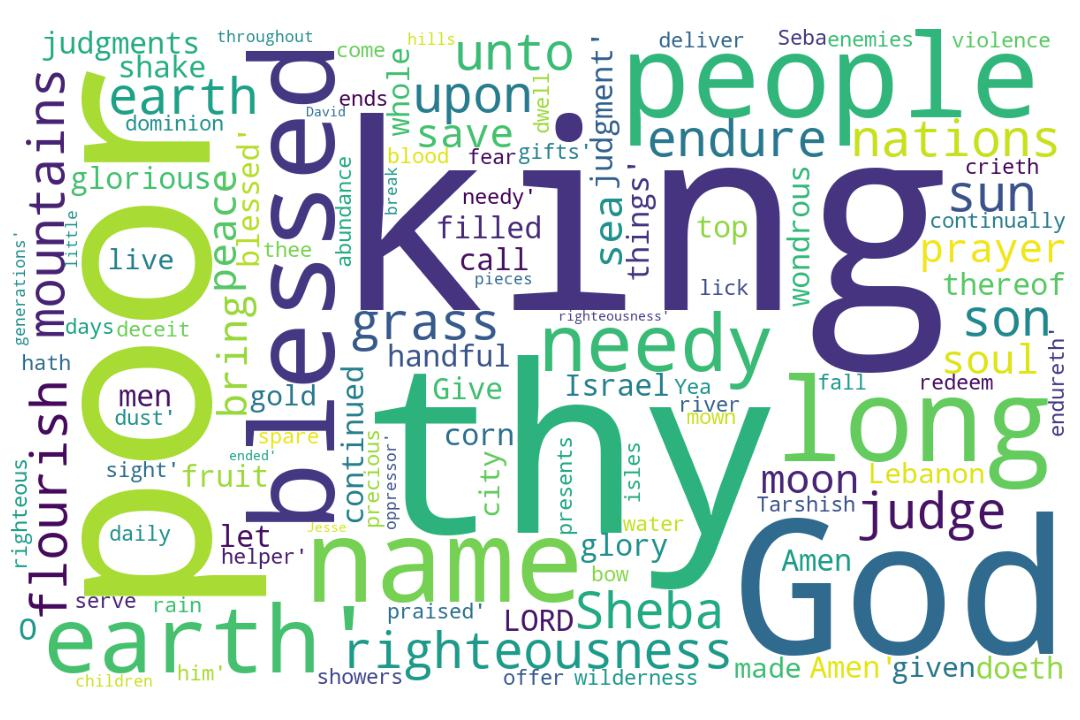
\includegraphics[width=\linewidth]{19OT-Psalms/Psalm72-WordCloud.jpg}
  \caption{Psalm 72 Word Cloud}
  \label{fig:Psalm 72 word Cloud}
\end{figure}


\marginpar{\scriptsize \centering \fcolorbox{bone}{lime}{\textbf{WITH THE PRINCE OF PEACE}}\\ (Psalm 72) \begin{compactenum}[I.][8]
    \item \textbf{Perfection in Judgment} \index[scripture]{Psalms!Psa 072:02}(Psa 72:2)
    \item The \textbf{Poor Blessed} \index[scripture]{Psalms!Psa 072:04}(Psa 72:4)
    \item \textbf{Peace Finally Arrives} \index[scripture]{Psalms!Psa 072:07}(Psa 72:7)
    \item \textbf{Opponents Praising} \index[scripture]{Psalms!Psa 072:09, 10}(Psa 72:9, 10)
    \item \textbf{Politics Centered on the Lord} \index[scripture]{Psalms!Psa 072:11}(Psa 72:11)
    \item \textbf{Produce Incredible} \index[scripture]{Psalms!Psa 072:16}(Psa 72:16)
    \item \textbf{Praise Continual} \index[scripture]{Psalms!Psa 072:17}(Psa 72:17)
\end{compactenum}}



\footnote{\textcolor[cmyk]{0.99998,1,0,0}{\hyperlink{TOC}{Return to end of Table of Contents.}}}\footnote{\href{https://audiobible.com/bible/psalms_72.html}{\textcolor[cmyk]{0.99998,1,0,0}{Psalm 72 Audio}}}\textcolor[cmyk]{0.99998,1,0,0}{\emph{A Psalm} for Solomon.}\\
\\
\textcolor[cmyk]{0.99998,1,0,0}{Give the king thy judgments, O God, and thy \fcolorbox{bone}{MYGOLD}{righteousness} unto the king's son.}
[2] \textcolor[cmyk]{0.99998,1,0,0}{He shall \fcolorbox{bone}{lime}{judge} thy people with \fcolorbox{bone}{MYGOLD}{righteousness}, and thy poor with judgment.}
[3] \textcolor[cmyk]{0.99998,1,0,0}{The mountains shall bring peace to the people, and the little hills, by \fcolorbox{bone}{MYGOLD}{righteousness}.}
[4] \textcolor[cmyk]{0.99998,1,0,0}{He shall judge the \fcolorbox{bone}{lime}{poor} of the people, he shall save the children of the needy, and shall break in pieces the oppressor.}
[5] \textcolor[cmyk]{0.99998,1,0,0}{They shall fear thee as long as the sun and moon endure, throughout all generations.}
[6] \textcolor[cmyk]{0.99998,1,0,0}{He shall come down like rain upon the mown grass: as showers \emph{that} water the earth.}
[7] \textcolor[cmyk]{0.99998,1,0,0}{In his days shall the righteous flourish; and abundance of \fcolorbox{bone}{lime}{peace} so long as the moon endureth.}
[8] \textcolor[cmyk]{0.99998,1,0,0}{He shall have dominion also from sea to sea, and from the river unto the ends of the earth.}\footnote{\textbf{Psalm 145:13} - Thy kingdom is an everlasting kingdom, and thy dominion endureth throughout all generations.}\footnote{\textbf{Zechariah 9:10} - And I will cut off the chariot from Ephraim, and the horse from Jerusalem, and the battle bow shall be cut off: and he shall speak peace unto the heathen: and his dominion shall be from sea even to sea, and from the river even to the ends of the earth.}\footnote{\textbf{Revelation 1:6} - And hath made us kings and priests unto God and his Father; to him be glory and dominion for ever and ever. Amen.}
[9] \textcolor[cmyk]{0.99998,1,0,0}{They that dwell in the wilderness shall \fcolorbox{bone}{lime}{bow before him}; and his enemies shall lick the dust.}
[10] \textcolor[cmyk]{0.99998,1,0,0}{The kings of Tarshish and of the isles shall bring presents: the kings of Sheba and Seba shall offer gifts.}
[11] \textcolor[cmyk]{0.99998,1,0,0}{Yea, all kings shall fall down \fcolorbox{bone}{lime}{before him}: all nations shall serve him.}
[12] \textcolor[cmyk]{0.99998,1,0,0}{For he shall deliver the needy when he crieth; the poor also, and \emph{him} that hath no helper.}
[13] \textcolor[cmyk]{0.99998,1,0,0}{He shall spare the poor and needy, and shall save the souls of the needy.}
[14] \textcolor[cmyk]{0.99998,1,0,0}{He shall redeem their soul from deceit and violence: and precious shall their blood be in his sight.}
[15] \textcolor[cmyk]{0.99998,1,0,0}{And he shall live, and to him shall be given of the gold of Sheba: prayer also shall be made for him continually; \emph{and} daily shall he be praised.}\footnote{\textbf{1 Kings 10:1-13} - And when the queen of Sheba heard of the fame of Solomon concerning the name of the LORD, she came to prove him with hard questions. [2] And she came to Jerusalem with a very great train, with camels that bare spices, and very much gold, and precious stones: and when she was come to Solomon, she communed with him of all that was in her heart. [3] And Solomon told her all her questions: there was not any thing hid from the king, which he told her not. [4] And when the queen of Sheba had seen all Solomon’s wisdom, and the house that he had built, [5] And the meat of his table, and the sitting of his servants, and the attendance of his ministers, and their apparel, and his cupbearers, and his ascent by which he went up unto the house of the LORD; there was no more spirit in her. [6] And she said to the king, It was a true report that I heard in mine own land of thy acts and of thy wisdom. [7] Howbeit I believed not the words, until I came, and mine eyes had seen it: and, behold, the half was not told me: thy wisdom and prosperity exceedeth the fame which I heard. [8] Happy are thy men, happy are these thy servants, which stand continually before thee, and that hear thy wisdom. [9] Blessed be the LORD thy God, which delighted in thee, to set thee on the throne of Israel: because the LORD loved Israel for ever, therefore made he thee king, to do judgment and justice. [10] And she gave the king an hundred and twenty talents of gold, and of spices very great store, and precious stones: there came no more such abundance of spices as these which the queen of Sheba gave to king Solomon. [11] And the navy also of Hiram, that brought gold from Ophir, brought in from Ophir great plenty of almug trees, and precious stones. [12] And the king made of the almug trees pillars for the house of the LORD, and for the king’s house, harps also and psalteries for singers: there came no such almug trees, nor were seen unto this day. [13] And king Solomon gave unto the queen of Sheba all her desire, whatsoever she asked, beside that which Solomon gave her of his royal bounty. So she turned and went to her own country, she and her servants.}\footnote{\textbf{Isaiah 60:6} - The multitude of camels shall cover thee, the dromedaries of Midian and Ephah; all they from Sheba shall come: they shall bring gold and incense; and they shall shew forth the praises of the LORD.}
[16] \textcolor[cmyk]{0.99998,1,0,0}{There shall be an handful of corn in the earth upon the top of the mountains; the \fcolorbox{bone}{lime}{fruit} thereof shall shake like Lebanon: and \emph{they} of the city shall flourish like grass of the earth.}
[17] \textcolor[cmyk]{0.99998,1,0,0}{His name shall endure for ever: his name shall be \fcolorbox{bone}{lime}{continued} as long as the sun: and \emph{men} shall be blessed in him: all nations shall call him blessed.}
[18] \textcolor[cmyk]{0.99998,1,0,0}{Blessed \emph{be} the LORD God, the God of Israel, who only doeth wondrous things.}
[19] \textcolor[cmyk]{0.99998,1,0,0}{And blessed \emph{be} his glorious name for ever: and let the whole earth be filled \emph{with} his glory; Amen, and Amen.}
[20] \textcolor[cmyk]{0.99998,1,0,0}{The prayers of David the son of Jesse are ended.}


\index[NWIV]{14!Psalms!Psa 72:1}\index[AWIP]{Give!Psalms!Psa 72:1}\index[AWIP]{the!Psalms!Psa 72:1}\index[AWIP]{the!Psalms!Psa 72:1 (2)}\index[AWIP]{king!Psalms!Psa 72:1}\index[AWIP]{thy!Psalms!Psa 72:1}\index[AWIP]{thy!Psalms!Psa 72:1 (2)}\index[AWIP]{judgments!Psalms!Psa 72:1}\index[AWIP]{O!Psalms!Psa 72:1}\index[AWIP]{God!Psalms!Psa 72:1}\index[AWIP]{and!Psalms!Psa 72:1}\index[AWIP]{righteousness!Psalms!Psa 72:1}\index[AWIP]{unto!Psalms!Psa 72:1}\index[AWIP]{king's!Psalms!Psa 72:1}\index[AWIP]{son!Psalms!Psa 72:1}

\index[NWIV]{12!Psalms!Psa 72:2}\index[AWIP]{He!Psalms!Psa 72:2}\index[AWIP]{shall!Psalms!Psa 72:2}\index[AWIP]{judge!Psalms!Psa 72:2}\index[AWIP]{thy!Psalms!Psa 72:2}\index[AWIP]{thy!Psalms!Psa 72:2 (2)}\index[AWIP]{people!Psalms!Psa 72:2}\index[AWIP]{with!Psalms!Psa 72:2}\index[AWIP]{with!Psalms!Psa 72:2 (2)}\index[AWIP]{righteousness!Psalms!Psa 72:2}\index[AWIP]{and!Psalms!Psa 72:2}\index[AWIP]{poor!Psalms!Psa 72:2}\index[AWIP]{judgment!Psalms!Psa 72:2}

\index[NWIV]{14!Psalms!Psa 72:3}\index[AWIP]{The!Psalms!Psa 72:3}\index[AWIP]{mountains!Psalms!Psa 72:3}\index[AWIP]{shall!Psalms!Psa 72:3}\index[AWIP]{bring!Psalms!Psa 72:3}\index[AWIP]{peace!Psalms!Psa 72:3}\index[AWIP]{to!Psalms!Psa 72:3}\index[AWIP]{the!Psalms!Psa 72:3}\index[AWIP]{the!Psalms!Psa 72:3 (2)}\index[AWIP]{people!Psalms!Psa 72:3}\index[AWIP]{and!Psalms!Psa 72:3}\index[AWIP]{little!Psalms!Psa 72:3}\index[AWIP]{hills!Psalms!Psa 72:3}\index[AWIP]{by!Psalms!Psa 72:3}\index[AWIP]{righteousness!Psalms!Psa 72:3}

\index[NWIV]{23!Psalms!Psa 72:4}\index[AWIP]{He!Psalms!Psa 72:4}\index[AWIP]{shall!Psalms!Psa 72:4}\index[AWIP]{shall!Psalms!Psa 72:4 (2)}\index[AWIP]{shall!Psalms!Psa 72:4 (3)}\index[AWIP]{judge!Psalms!Psa 72:4}\index[AWIP]{the!Psalms!Psa 72:4}\index[AWIP]{the!Psalms!Psa 72:4 (2)}\index[AWIP]{the!Psalms!Psa 72:4 (3)}\index[AWIP]{the!Psalms!Psa 72:4 (4)}\index[AWIP]{the!Psalms!Psa 72:4 (5)}\index[AWIP]{poor!Psalms!Psa 72:4}\index[AWIP]{of!Psalms!Psa 72:4}\index[AWIP]{of!Psalms!Psa 72:4 (2)}\index[AWIP]{people!Psalms!Psa 72:4}\index[AWIP]{he!Psalms!Psa 72:4}\index[AWIP]{save!Psalms!Psa 72:4}\index[AWIP]{children!Psalms!Psa 72:4}\index[AWIP]{needy!Psalms!Psa 72:4}\index[AWIP]{and!Psalms!Psa 72:4}\index[AWIP]{break!Psalms!Psa 72:4}\index[AWIP]{in!Psalms!Psa 72:4}\index[AWIP]{pieces!Psalms!Psa 72:4}\index[AWIP]{oppressor!Psalms!Psa 72:4}

\index[NWIV]{15!Psalms!Psa 72:5}\index[AWIP]{They!Psalms!Psa 72:5}\index[AWIP]{shall!Psalms!Psa 72:5}\index[AWIP]{fear!Psalms!Psa 72:5}\index[AWIP]{thee!Psalms!Psa 72:5}\index[AWIP]{as!Psalms!Psa 72:5}\index[AWIP]{as!Psalms!Psa 72:5 (2)}\index[AWIP]{long!Psalms!Psa 72:5}\index[AWIP]{the!Psalms!Psa 72:5}\index[AWIP]{sun!Psalms!Psa 72:5}\index[AWIP]{and!Psalms!Psa 72:5}\index[AWIP]{moon!Psalms!Psa 72:5}\index[AWIP]{endure!Psalms!Psa 72:5}\index[AWIP]{throughout!Psalms!Psa 72:5}\index[AWIP]{all!Psalms!Psa 72:5}\index[AWIP]{generations!Psalms!Psa 72:5}

\index[NWIV]{16!Psalms!Psa 72:6}\index[AWIP]{He!Psalms!Psa 72:6}\index[AWIP]{shall!Psalms!Psa 72:6}\index[AWIP]{come!Psalms!Psa 72:6}\index[AWIP]{down!Psalms!Psa 72:6}\index[AWIP]{like!Psalms!Psa 72:6}\index[AWIP]{rain!Psalms!Psa 72:6}\index[AWIP]{upon!Psalms!Psa 72:6}\index[AWIP]{the!Psalms!Psa 72:6}\index[AWIP]{the!Psalms!Psa 72:6 (2)}\index[AWIP]{mown!Psalms!Psa 72:6}\index[AWIP]{grass!Psalms!Psa 72:6}\index[AWIP]{as!Psalms!Psa 72:6}\index[AWIP]{showers!Psalms!Psa 72:6}\index[AWIP]{\emph{that}!Psalms!Psa 72:6}\index[AWIP]{water!Psalms!Psa 72:6}\index[AWIP]{earth!Psalms!Psa 72:6}\index[AWIP]{\emph{that}!Psalms!Psa 72:6}

\index[NWIV]{17!Psalms!Psa 72:7}\index[AWIP]{In!Psalms!Psa 72:7}\index[AWIP]{his!Psalms!Psa 72:7}\index[AWIP]{days!Psalms!Psa 72:7}\index[AWIP]{shall!Psalms!Psa 72:7}\index[AWIP]{the!Psalms!Psa 72:7}\index[AWIP]{the!Psalms!Psa 72:7 (2)}\index[AWIP]{righteous!Psalms!Psa 72:7}\index[AWIP]{flourish!Psalms!Psa 72:7}\index[AWIP]{and!Psalms!Psa 72:7}\index[AWIP]{abundance!Psalms!Psa 72:7}\index[AWIP]{of!Psalms!Psa 72:7}\index[AWIP]{peace!Psalms!Psa 72:7}\index[AWIP]{so!Psalms!Psa 72:7}\index[AWIP]{long!Psalms!Psa 72:7}\index[AWIP]{as!Psalms!Psa 72:7}\index[AWIP]{moon!Psalms!Psa 72:7}\index[AWIP]{endureth!Psalms!Psa 72:7}

\index[NWIV]{19!Psalms!Psa 72:8}\index[AWIP]{He!Psalms!Psa 72:8}\index[AWIP]{shall!Psalms!Psa 72:8}\index[AWIP]{have!Psalms!Psa 72:8}\index[AWIP]{dominion!Psalms!Psa 72:8}\index[AWIP]{also!Psalms!Psa 72:8}\index[AWIP]{from!Psalms!Psa 72:8}\index[AWIP]{from!Psalms!Psa 72:8 (2)}\index[AWIP]{sea!Psalms!Psa 72:8}\index[AWIP]{sea!Psalms!Psa 72:8 (2)}\index[AWIP]{to!Psalms!Psa 72:8}\index[AWIP]{and!Psalms!Psa 72:8}\index[AWIP]{the!Psalms!Psa 72:8}\index[AWIP]{the!Psalms!Psa 72:8 (2)}\index[AWIP]{the!Psalms!Psa 72:8 (3)}\index[AWIP]{river!Psalms!Psa 72:8}\index[AWIP]{unto!Psalms!Psa 72:8}\index[AWIP]{ends!Psalms!Psa 72:8}\index[AWIP]{of!Psalms!Psa 72:8}\index[AWIP]{earth!Psalms!Psa 72:8}

\index[NWIV]{17!Psalms!Psa 72:9}\index[AWIP]{They!Psalms!Psa 72:9}\index[AWIP]{that!Psalms!Psa 72:9}\index[AWIP]{dwell!Psalms!Psa 72:9}\index[AWIP]{in!Psalms!Psa 72:9}\index[AWIP]{the!Psalms!Psa 72:9}\index[AWIP]{the!Psalms!Psa 72:9 (2)}\index[AWIP]{wilderness!Psalms!Psa 72:9}\index[AWIP]{shall!Psalms!Psa 72:9}\index[AWIP]{shall!Psalms!Psa 72:9 (2)}\index[AWIP]{bow!Psalms!Psa 72:9}\index[AWIP]{before!Psalms!Psa 72:9}\index[AWIP]{him!Psalms!Psa 72:9}\index[AWIP]{and!Psalms!Psa 72:9}\index[AWIP]{his!Psalms!Psa 72:9}\index[AWIP]{enemies!Psalms!Psa 72:9}\index[AWIP]{lick!Psalms!Psa 72:9}\index[AWIP]{dust!Psalms!Psa 72:9}

\index[NWIV]{20!Psalms!Psa 72:10}\index[AWIP]{The!Psalms!Psa 72:10}\index[AWIP]{kings!Psalms!Psa 72:10}\index[AWIP]{kings!Psalms!Psa 72:10 (2)}\index[AWIP]{of!Psalms!Psa 72:10}\index[AWIP]{of!Psalms!Psa 72:10 (2)}\index[AWIP]{of!Psalms!Psa 72:10 (3)}\index[AWIP]{Tarshish!Psalms!Psa 72:10}\index[AWIP]{and!Psalms!Psa 72:10}\index[AWIP]{and!Psalms!Psa 72:10 (2)}\index[AWIP]{the!Psalms!Psa 72:10}\index[AWIP]{the!Psalms!Psa 72:10 (2)}\index[AWIP]{isles!Psalms!Psa 72:10}\index[AWIP]{shall!Psalms!Psa 72:10}\index[AWIP]{shall!Psalms!Psa 72:10 (2)}\index[AWIP]{bring!Psalms!Psa 72:10}\index[AWIP]{presents!Psalms!Psa 72:10}\index[AWIP]{Sheba!Psalms!Psa 72:10}\index[AWIP]{Seba!Psalms!Psa 72:10}\index[AWIP]{offer!Psalms!Psa 72:10}\index[AWIP]{gifts!Psalms!Psa 72:10}

\index[NWIV]{13!Psalms!Psa 72:11}\index[AWIP]{Yea!Psalms!Psa 72:11}\index[AWIP]{all!Psalms!Psa 72:11}\index[AWIP]{all!Psalms!Psa 72:11 (2)}\index[AWIP]{kings!Psalms!Psa 72:11}\index[AWIP]{shall!Psalms!Psa 72:11}\index[AWIP]{shall!Psalms!Psa 72:11 (2)}\index[AWIP]{fall!Psalms!Psa 72:11}\index[AWIP]{down!Psalms!Psa 72:11}\index[AWIP]{before!Psalms!Psa 72:11}\index[AWIP]{him!Psalms!Psa 72:11}\index[AWIP]{him!Psalms!Psa 72:11 (2)}\index[AWIP]{nations!Psalms!Psa 72:11}\index[AWIP]{serve!Psalms!Psa 72:11}

\index[NWIV]{18!Psalms!Psa 72:12}\index[AWIP]{For!Psalms!Psa 72:12}\index[AWIP]{he!Psalms!Psa 72:12}\index[AWIP]{he!Psalms!Psa 72:12 (2)}\index[AWIP]{shall!Psalms!Psa 72:12}\index[AWIP]{deliver!Psalms!Psa 72:12}\index[AWIP]{the!Psalms!Psa 72:12}\index[AWIP]{the!Psalms!Psa 72:12 (2)}\index[AWIP]{needy!Psalms!Psa 72:12}\index[AWIP]{when!Psalms!Psa 72:12}\index[AWIP]{crieth!Psalms!Psa 72:12}\index[AWIP]{poor!Psalms!Psa 72:12}\index[AWIP]{also!Psalms!Psa 72:12}\index[AWIP]{and!Psalms!Psa 72:12}\index[AWIP]{\emph{him}!Psalms!Psa 72:12}\index[AWIP]{that!Psalms!Psa 72:12}\index[AWIP]{hath!Psalms!Psa 72:12}\index[AWIP]{no!Psalms!Psa 72:12}\index[AWIP]{helper!Psalms!Psa 72:12}\index[AWIP]{\emph{him}!Psalms!Psa 72:12}

\index[NWIV]{15!Psalms!Psa 72:13}\index[AWIP]{He!Psalms!Psa 72:13}\index[AWIP]{shall!Psalms!Psa 72:13}\index[AWIP]{shall!Psalms!Psa 72:13 (2)}\index[AWIP]{spare!Psalms!Psa 72:13}\index[AWIP]{the!Psalms!Psa 72:13}\index[AWIP]{the!Psalms!Psa 72:13 (2)}\index[AWIP]{the!Psalms!Psa 72:13 (3)}\index[AWIP]{poor!Psalms!Psa 72:13}\index[AWIP]{and!Psalms!Psa 72:13}\index[AWIP]{and!Psalms!Psa 72:13 (2)}\index[AWIP]{needy!Psalms!Psa 72:13}\index[AWIP]{needy!Psalms!Psa 72:13 (2)}\index[AWIP]{save!Psalms!Psa 72:13}\index[AWIP]{souls!Psalms!Psa 72:13}\index[AWIP]{of!Psalms!Psa 72:13}

\index[NWIV]{18!Psalms!Psa 72:14}\index[AWIP]{He!Psalms!Psa 72:14}\index[AWIP]{shall!Psalms!Psa 72:14}\index[AWIP]{shall!Psalms!Psa 72:14 (2)}\index[AWIP]{redeem!Psalms!Psa 72:14}\index[AWIP]{their!Psalms!Psa 72:14}\index[AWIP]{their!Psalms!Psa 72:14 (2)}\index[AWIP]{soul!Psalms!Psa 72:14}\index[AWIP]{from!Psalms!Psa 72:14}\index[AWIP]{deceit!Psalms!Psa 72:14}\index[AWIP]{and!Psalms!Psa 72:14}\index[AWIP]{and!Psalms!Psa 72:14 (2)}\index[AWIP]{violence!Psalms!Psa 72:14}\index[AWIP]{precious!Psalms!Psa 72:14}\index[AWIP]{blood!Psalms!Psa 72:14}\index[AWIP]{be!Psalms!Psa 72:14}\index[AWIP]{in!Psalms!Psa 72:14}\index[AWIP]{his!Psalms!Psa 72:14}\index[AWIP]{sight!Psalms!Psa 72:14}

\index[NWIV]{29!Psalms!Psa 72:15}\index[AWIP]{And!Psalms!Psa 72:15}\index[AWIP]{he!Psalms!Psa 72:15}\index[AWIP]{he!Psalms!Psa 72:15 (2)}\index[AWIP]{shall!Psalms!Psa 72:15}\index[AWIP]{shall!Psalms!Psa 72:15 (2)}\index[AWIP]{shall!Psalms!Psa 72:15 (3)}\index[AWIP]{shall!Psalms!Psa 72:15 (4)}\index[AWIP]{live!Psalms!Psa 72:15}\index[AWIP]{and!Psalms!Psa 72:15}\index[AWIP]{to!Psalms!Psa 72:15}\index[AWIP]{him!Psalms!Psa 72:15}\index[AWIP]{him!Psalms!Psa 72:15 (2)}\index[AWIP]{be!Psalms!Psa 72:15}\index[AWIP]{be!Psalms!Psa 72:15 (2)}\index[AWIP]{be!Psalms!Psa 72:15 (3)}\index[AWIP]{given!Psalms!Psa 72:15}\index[AWIP]{of!Psalms!Psa 72:15}\index[AWIP]{of!Psalms!Psa 72:15 (2)}\index[AWIP]{the!Psalms!Psa 72:15}\index[AWIP]{gold!Psalms!Psa 72:15}\index[AWIP]{Sheba!Psalms!Psa 72:15}\index[AWIP]{prayer!Psalms!Psa 72:15}\index[AWIP]{also!Psalms!Psa 72:15}\index[AWIP]{made!Psalms!Psa 72:15}\index[AWIP]{for!Psalms!Psa 72:15}\index[AWIP]{continually!Psalms!Psa 72:15}\index[AWIP]{\emph{and}!Psalms!Psa 72:15}\index[AWIP]{daily!Psalms!Psa 72:15}\index[AWIP]{praised!Psalms!Psa 72:15}\index[AWIP]{\emph{and}!Psalms!Psa 72:15}

\index[NWIV]{35!Psalms!Psa 72:16}\index[AWIP]{There!Psalms!Psa 72:16}\index[AWIP]{shall!Psalms!Psa 72:16}\index[AWIP]{shall!Psalms!Psa 72:16 (2)}\index[AWIP]{shall!Psalms!Psa 72:16 (3)}\index[AWIP]{be!Psalms!Psa 72:16}\index[AWIP]{an!Psalms!Psa 72:16}\index[AWIP]{handful!Psalms!Psa 72:16}\index[AWIP]{of!Psalms!Psa 72:16}\index[AWIP]{of!Psalms!Psa 72:16 (2)}\index[AWIP]{of!Psalms!Psa 72:16 (3)}\index[AWIP]{of!Psalms!Psa 72:16 (4)}\index[AWIP]{corn!Psalms!Psa 72:16}\index[AWIP]{in!Psalms!Psa 72:16}\index[AWIP]{the!Psalms!Psa 72:16}\index[AWIP]{the!Psalms!Psa 72:16 (2)}\index[AWIP]{the!Psalms!Psa 72:16 (3)}\index[AWIP]{the!Psalms!Psa 72:16 (4)}\index[AWIP]{the!Psalms!Psa 72:16 (5)}\index[AWIP]{the!Psalms!Psa 72:16 (6)}\index[AWIP]{earth!Psalms!Psa 72:16}\index[AWIP]{earth!Psalms!Psa 72:16 (2)}\index[AWIP]{upon!Psalms!Psa 72:16}\index[AWIP]{top!Psalms!Psa 72:16}\index[AWIP]{mountains!Psalms!Psa 72:16}\index[AWIP]{fruit!Psalms!Psa 72:16}\index[AWIP]{thereof!Psalms!Psa 72:16}\index[AWIP]{shake!Psalms!Psa 72:16}\index[AWIP]{like!Psalms!Psa 72:16}\index[AWIP]{like!Psalms!Psa 72:16 (2)}\index[AWIP]{Lebanon!Psalms!Psa 72:16}\index[AWIP]{and!Psalms!Psa 72:16}\index[AWIP]{\emph{they}!Psalms!Psa 72:16}\index[AWIP]{city!Psalms!Psa 72:16}\index[AWIP]{flourish!Psalms!Psa 72:16}\index[AWIP]{grass!Psalms!Psa 72:16}\index[AWIP]{\emph{they}!Psalms!Psa 72:16}

\index[NWIV]{29!Psalms!Psa 72:17}\index[AWIP]{His!Psalms!Psa 72:17}\index[AWIP]{name!Psalms!Psa 72:17}\index[AWIP]{name!Psalms!Psa 72:17 (2)}\index[AWIP]{shall!Psalms!Psa 72:17}\index[AWIP]{shall!Psalms!Psa 72:17 (2)}\index[AWIP]{shall!Psalms!Psa 72:17 (3)}\index[AWIP]{shall!Psalms!Psa 72:17 (4)}\index[AWIP]{endure!Psalms!Psa 72:17}\index[AWIP]{for!Psalms!Psa 72:17}\index[AWIP]{ever!Psalms!Psa 72:17}\index[AWIP]{his!Psalms!Psa 72:17}\index[AWIP]{be!Psalms!Psa 72:17}\index[AWIP]{be!Psalms!Psa 72:17 (2)}\index[AWIP]{continued!Psalms!Psa 72:17}\index[AWIP]{as!Psalms!Psa 72:17}\index[AWIP]{as!Psalms!Psa 72:17 (2)}\index[AWIP]{long!Psalms!Psa 72:17}\index[AWIP]{the!Psalms!Psa 72:17}\index[AWIP]{sun!Psalms!Psa 72:17}\index[AWIP]{and!Psalms!Psa 72:17}\index[AWIP]{\emph{men}!Psalms!Psa 72:17}\index[AWIP]{blessed!Psalms!Psa 72:17}\index[AWIP]{blessed!Psalms!Psa 72:17 (2)}\index[AWIP]{in!Psalms!Psa 72:17}\index[AWIP]{him!Psalms!Psa 72:17}\index[AWIP]{him!Psalms!Psa 72:17 (2)}\index[AWIP]{all!Psalms!Psa 72:17}\index[AWIP]{nations!Psalms!Psa 72:17}\index[AWIP]{call!Psalms!Psa 72:17}\index[AWIP]{\emph{men}!Psalms!Psa 72:17}

\index[NWIV]{14!Psalms!Psa 72:18}\index[AWIP]{Blessed!Psalms!Psa 72:18}\index[AWIP]{\emph{be}!Psalms!Psa 72:18}\index[AWIP]{the!Psalms!Psa 72:18}\index[AWIP]{the!Psalms!Psa 72:18 (2)}\index[AWIP]{LORD!Psalms!Psa 72:18}\index[AWIP]{God!Psalms!Psa 72:18}\index[AWIP]{God!Psalms!Psa 72:18 (2)}\index[AWIP]{of!Psalms!Psa 72:18}\index[AWIP]{Israel!Psalms!Psa 72:18}\index[AWIP]{who!Psalms!Psa 72:18}\index[AWIP]{only!Psalms!Psa 72:18}\index[AWIP]{doeth!Psalms!Psa 72:18}\index[AWIP]{wondrous!Psalms!Psa 72:18}\index[AWIP]{things!Psalms!Psa 72:18}\index[AWIP]{\emph{be}!Psalms!Psa 72:18}

\index[NWIV]{21!Psalms!Psa 72:19}\index[AWIP]{And!Psalms!Psa 72:19}\index[AWIP]{blessed!Psalms!Psa 72:19}\index[AWIP]{\emph{be}!Psalms!Psa 72:19}\index[AWIP]{his!Psalms!Psa 72:19}\index[AWIP]{his!Psalms!Psa 72:19 (2)}\index[AWIP]{glorious!Psalms!Psa 72:19}\index[AWIP]{name!Psalms!Psa 72:19}\index[AWIP]{for!Psalms!Psa 72:19}\index[AWIP]{ever!Psalms!Psa 72:19}\index[AWIP]{and!Psalms!Psa 72:19}\index[AWIP]{and!Psalms!Psa 72:19 (2)}\index[AWIP]{let!Psalms!Psa 72:19}\index[AWIP]{the!Psalms!Psa 72:19}\index[AWIP]{whole!Psalms!Psa 72:19}\index[AWIP]{earth!Psalms!Psa 72:19}\index[AWIP]{be!Psalms!Psa 72:19}\index[AWIP]{filled!Psalms!Psa 72:19}\index[AWIP]{\emph{with}!Psalms!Psa 72:19}\index[AWIP]{glory!Psalms!Psa 72:19}\index[AWIP]{Amen!Psalms!Psa 72:19}\index[AWIP]{Amen!Psalms!Psa 72:19 (2)}\index[AWIP]{\emph{be}!Psalms!Psa 72:19}\index[AWIP]{\emph{with}!Psalms!Psa 72:19}

\index[NWIV]{10!Psalms!Psa 72:20}\index[AWIP]{The!Psalms!Psa 72:20}\index[AWIP]{prayers!Psalms!Psa 72:20}\index[AWIP]{of!Psalms!Psa 72:20}\index[AWIP]{of!Psalms!Psa 72:20 (2)}\index[AWIP]{David!Psalms!Psa 72:20}\index[AWIP]{the!Psalms!Psa 72:20}\index[AWIP]{son!Psalms!Psa 72:20}\index[AWIP]{Jesse!Psalms!Psa 72:20}\index[AWIP]{are!Psalms!Psa 72:20}\index[AWIP]{ended!Psalms!Psa 72:20}


\section{Psalm 72 Outlines}

\subsection{My Outlines}

\subsubsection{Perfect Peace with the Prince of Peace}

\index[speaker]{Keith Anthony!Psalm 072 (Perfect Peace with the Prince of Peace)}
\index[series]{Psalms (Keith Anthony)!Psalm 072 (Perfect Peace with the Prince of Peace)}
\index[date]{2017/03/13!Psalm 072 (Perfect Peace with the Prince of Peace) (Keith Anthony)}

\begin{compactenum}[I.][8]
    \item \textbf{Perfection in Judgment} \index[scripture]{Psalms!Psa 072:02}(Psa 72:2)
    \item The \textbf{Poor Blessed} \index[scripture]{Psalms!Psa 072:04}(Psa 72:4)
    \item \textbf{Peace Finally Arrives} \index[scripture]{Psalms!Psa 072:07}(Psa 72:7)
    \item \textbf{Oponents Praising} \index[scripture]{Psalms!Psa 072:09, 10}(Psa 72:9, 10)
    \item \textbf{Politics Centered on the Lord} \index[scripture]{Psalms!Psa 072:11}(Psa 72:11)
    \item \textbf{Produce Incredible} \index[scripture]{Psalms!Psa 072:16}(Psa 72:16)
    \item \textbf{Praise Continual} \index[scripture]{Psalms!Psa 072:17}(Psa 72:17)
\end{compactenum}





\subsection{Outlines from Others}


\section{Psalm 72 Comments}

\subsection{Numeric Nuggets}
Verse 11 has 13 words. Verse 3 has 13 unique words. the 13-letter word ``righteousness'' is used in Psalm 72.
\subsection{Psalm 72 Repeated Phrases}


%%%%%%%%%%
%%%%%%%%%%
\normalsize
 
\begin{center}
\begin{longtable}{|p{3.0in}|p{0.5in}|}
\caption[Psalm 72 Repeated Phrases]{Psalm 72 Repeated Phrases}\label{table:Repeated Phrases Psalm 72} \\
\hline \multicolumn{1}{|c|}{\textbf{Phrase}} & \multicolumn{1}{c|}{\textbf{Frequency}} \\ \hline 
\endfirsthead
 
\multicolumn{2}{c}
{{\bfseries \tablename\ \thetable{} -- continued from previous page}} \\  
\hline \multicolumn{1}{|c|}{\textbf{Phrase}} & \multicolumn{1}{c|}{\textbf{Frequency}} \\ \hline 
\endhead
 
\hline \multicolumn{2}{c}{{ }} \\ \hline
\endfoot 
of the & 9\\ \hline 
He shall & 6\\ \hline 
shall be & 5\\ \hline 
the earth & 4\\ \hline 
the poor & 3\\ \hline 
he shall & 3\\ \hline 
the needy & 3\\ \hline 
long as & 3\\ \hline 
long as the & 3\\ \hline 
as the & 3\\ \hline 
\end{longtable}
\end{center}



%%%%%%%%%%
%%%%%%%%%%



\section{Psalm 72 Word Statistics}


%%%%%%%%%%
%%%%%%%%%%
\normalsize
 
\begin{center}
\begin{longtable}{l|c|c|c|c}
\caption[Psalm 72 Statistics]{Psalm 72 Statistics}\label{table:Statistics for Psalm 72} \\
\hline \multicolumn{1}{|c|}{\textbf{Verse(s)}} & \multicolumn{1}{|c|}{\textbf{Count}} & \multicolumn{1}{|c|}{\textbf{Unique}} & \multicolumn{1}{|c|}{\textbf{Italics}} & \multicolumn{1}{|c|}{\textbf{Uniq Italic}}  \\ \hline 
\endfirsthead
 
\multicolumn{5}{c}
{{\bfseries \tablename\ \thetable{} -- continued from previous page}} \\  
\hline \multicolumn{1}{|c|}{\textbf{Verse(s)}} & \multicolumn{1}{|c|}{\textbf{Count}} & \multicolumn{1}{|c|}{\textbf{Unique}} & \multicolumn{1}{|c|}{\textbf{Italics}} & \multicolumn{1}{|c|}{\textbf{Uniq Italic}}  \\ \hline 
\endhead
 
\hline \multicolumn{5}{|r|}{{Continued if needed}} \\ \hline
\endfoot 
1 & 14 & 12 & 0 & 0\\ \hline
2 & 12 & 10 & 0 & 0\\ \hline
3 & 14 & 13 & 0 & 0\\ \hline
4 & 23 & 16 & 0 & 0\\ \hline
5 & 15 & 14 & 0 & 0\\ \hline
6 & 16 & 15 & 1 & 1\\ \hline
7 & 17 & 16 & 0 & 0\\ \hline
8 & 19 & 15 & 0 & 0\\ \hline
9 & 17 & 15 & 0 & 0\\ \hline
10 & 20 & 14 & 0 & 0\\ \hline
11 & 13 & 10 & 0 & 0\\ \hline
12 & 18 & 16 & 1 & 1\\ \hline
13 & 15 & 10 & 0 & 0\\ \hline
14 & 18 & 15 & 0 & 0\\ \hline
15 & 29 & 21 & 1 & 1\\ \hline
16 & 35 & 23 & 1 & 1\\ \hline
17 & 29 & 21 & 1 & 1\\ \hline
18 & 14 & 12 & 1 & 1\\ \hline
19 & 21 & 18 & 2 & 2\\ \hline
20 & 10 & 9 & 0 & 0\\ \hline
Total & 369 & 163 & 8 & 7
\end{longtable}
\end{center}



%%%%%%%%%%
%%%%%%%%%%


\subsection{Psalm 72 Words by Frequency}


%%%%%%%%%%
%%%%%%%%%%
\normalsize
 
\begin{center}
\begin{longtable}{l|r}
\caption[Psalm 72 Words by Frequency]{Psalm 72 Words by Frequency}\label{table:WordsbyFrequency for Psalm 72} \\
\hline \multicolumn{1}{|c|}{\textbf{Word}} & \multicolumn{1}{c|}{\textbf{Frequency}} \\ \hline 
\endfirsthead
 
\multicolumn{2}{c}
{{\bfseries \tablename\ \thetable{} -- continued from previous page}} \\  
\hline \multicolumn{1}{|c|}{\textbf{Word}} & \multicolumn{1}{c|}{\textbf{Frequency}} \\ \hline 
\endhead
 
\hline \multicolumn{2}{c}{{ }} \\ \hline
\endfoot 
the & 38\\ \hline 
shall & 31\\ \hline 
and & 20\\ \hline 
of & 17\\ \hline 
be & 8\\ \hline 
him & 7\\ \hline 
He & 6\\ \hline 
as & 6\\ \hline 
his & 6\\ \hline 
he & 5\\ \hline 
in & 5\\ \hline 
earth & 5\\ \hline 
thy & 4\\ \hline 
poor & 4\\ \hline 
needy & 4\\ \hline 
all & 4\\ \hline 
God & 3\\ \hline 
righteousness & 3\\ \hline 
people & 3\\ \hline 
The & 3\\ \hline 
to & 3\\ \hline 
long & 3\\ \hline 
like & 3\\ \hline 
also & 3\\ \hline 
from & 3\\ \hline 
kings & 3\\ \hline 
for & 3\\ \hline 
name & 3\\ \hline 
blessed & 3\\ \hline 
unto & 2\\ \hline 
son & 2\\ \hline 
judge & 2\\ \hline 
with & 2\\ \hline 
mountains & 2\\ \hline 
bring & 2\\ \hline 
peace & 2\\ \hline 
save & 2\\ \hline 
They & 2\\ \hline 
sun & 2\\ \hline 
moon & 2\\ \hline 
endure & 2\\ \hline 
down & 2\\ \hline 
upon & 2\\ \hline 
grass & 2\\ \hline 
flourish & 2\\ \hline 
sea & 2\\ \hline 
that & 2\\ \hline 
before & 2\\ \hline 
Sheba & 2\\ \hline 
nations & 2\\ \hline 
their & 2\\ \hline 
And & 2\\ \hline 
ever & 2\\ \hline 
\emph{be} & 2\\ \hline 
Amen & 2\\ \hline 
Give & 1\\ \hline 
king & 1\\ \hline 
judgments & 1\\ \hline 
O & 1\\ \hline 
king's & 1\\ \hline 
judgment & 1\\ \hline 
little & 1\\ \hline 
hills & 1\\ \hline 
by & 1\\ \hline 
children & 1\\ \hline 
break & 1\\ \hline 
pieces & 1\\ \hline 
oppressor & 1\\ \hline 
fear & 1\\ \hline 
thee & 1\\ \hline 
throughout & 1\\ \hline 
generations & 1\\ \hline 
come & 1\\ \hline 
rain & 1\\ \hline 
mown & 1\\ \hline 
showers & 1\\ \hline 
\emph{that} & 1\\ \hline 
water & 1\\ \hline 
In & 1\\ \hline 
days & 1\\ \hline 
righteous & 1\\ \hline 
abundance & 1\\ \hline 
so & 1\\ \hline 
endureth & 1\\ \hline 
have & 1\\ \hline 
dominion & 1\\ \hline 
river & 1\\ \hline 
ends & 1\\ \hline 
dwell & 1\\ \hline 
wilderness & 1\\ \hline 
bow & 1\\ \hline 
enemies & 1\\ \hline 
lick & 1\\ \hline 
dust & 1\\ \hline 
Tarshish & 1\\ \hline 
isles & 1\\ \hline 
presents & 1\\ \hline 
Seba & 1\\ \hline 
offer & 1\\ \hline 
gifts & 1\\ \hline 
Yea & 1\\ \hline 
fall & 1\\ \hline 
serve & 1\\ \hline 
For & 1\\ \hline 
deliver & 1\\ \hline 
when & 1\\ \hline 
crieth & 1\\ \hline 
\emph{him} & 1\\ \hline 
hath & 1\\ \hline 
no & 1\\ \hline 
helper & 1\\ \hline 
spare & 1\\ \hline 
souls & 1\\ \hline 
redeem & 1\\ \hline 
soul & 1\\ \hline 
deceit & 1\\ \hline 
violence & 1\\ \hline 
precious & 1\\ \hline 
blood & 1\\ \hline 
sight & 1\\ \hline 
live & 1\\ \hline 
given & 1\\ \hline 
gold & 1\\ \hline 
prayer & 1\\ \hline 
made & 1\\ \hline 
continually & 1\\ \hline 
\emph{and} & 1\\ \hline 
daily & 1\\ \hline 
praised & 1\\ \hline 
There & 1\\ \hline 
an & 1\\ \hline 
handful & 1\\ \hline 
corn & 1\\ \hline 
top & 1\\ \hline 
fruit & 1\\ \hline 
thereof & 1\\ \hline 
shake & 1\\ \hline 
Lebanon & 1\\ \hline 
\emph{they} & 1\\ \hline 
city & 1\\ \hline 
His & 1\\ \hline 
continued & 1\\ \hline 
\emph{men} & 1\\ \hline 
call & 1\\ \hline 
Blessed & 1\\ \hline 
LORD & 1\\ \hline 
Israel & 1\\ \hline 
who & 1\\ \hline 
only & 1\\ \hline 
doeth & 1\\ \hline 
wondrous & 1\\ \hline 
things & 1\\ \hline 
glorious & 1\\ \hline 
let & 1\\ \hline 
whole & 1\\ \hline 
filled & 1\\ \hline 
\emph{with} & 1\\ \hline 
glory & 1\\ \hline 
prayers & 1\\ \hline 
David & 1\\ \hline 
Jesse & 1\\ \hline 
are & 1\\ \hline 
ended & 1\\ \hline 
\end{longtable}
\end{center}



%%%%%%%%%%
%%%%%%%%%%


\subsection{Psalm 72 Words Alphabetically}


%%%%%%%%%%
%%%%%%%%%%
\normalsize
 
\begin{center}
\begin{longtable}{l|r}
\caption[Psalm 72 Words Alphabetically]{Psalm 72 Words Alphabetically}\label{table:WordsAlphabetically for Psalm 72} \\
\hline \multicolumn{1}{|c|}{\textbf{Word}} & \multicolumn{1}{c|}{\textbf{Frequency}} \\ \hline 
\endfirsthead
 
\multicolumn{2}{c}
{{\bfseries \tablename\ \thetable{} -- continued from previous page}} \\  
\hline \multicolumn{1}{|c|}{\textbf{Word}} & \multicolumn{1}{c|}{\textbf{Frequency}} \\ \hline 
\endhead
 
\hline \multicolumn{2}{c}{{ }} \\ \hline
\endfoot 
Amen & 2\\ \hline 
And & 2\\ \hline 
Blessed & 1\\ \hline 
David & 1\\ \hline 
For & 1\\ \hline 
Give & 1\\ \hline 
God & 3\\ \hline 
He & 6\\ \hline 
His & 1\\ \hline 
In & 1\\ \hline 
Israel & 1\\ \hline 
Jesse & 1\\ \hline 
LORD & 1\\ \hline 
Lebanon & 1\\ \hline 
O & 1\\ \hline 
Seba & 1\\ \hline 
Sheba & 2\\ \hline 
Tarshish & 1\\ \hline 
The & 3\\ \hline 
There & 1\\ \hline 
They & 2\\ \hline 
Yea & 1\\ \hline 
\emph{and} & 1\\ \hline 
\emph{be} & 2\\ \hline 
\emph{him} & 1\\ \hline 
\emph{men} & 1\\ \hline 
\emph{that} & 1\\ \hline 
\emph{they} & 1\\ \hline 
\emph{with} & 1\\ \hline 
abundance & 1\\ \hline 
all & 4\\ \hline 
also & 3\\ \hline 
an & 1\\ \hline 
and & 20\\ \hline 
are & 1\\ \hline 
as & 6\\ \hline 
be & 8\\ \hline 
before & 2\\ \hline 
blessed & 3\\ \hline 
blood & 1\\ \hline 
bow & 1\\ \hline 
break & 1\\ \hline 
bring & 2\\ \hline 
by & 1\\ \hline 
call & 1\\ \hline 
children & 1\\ \hline 
city & 1\\ \hline 
come & 1\\ \hline 
continually & 1\\ \hline 
continued & 1\\ \hline 
corn & 1\\ \hline 
crieth & 1\\ \hline 
daily & 1\\ \hline 
days & 1\\ \hline 
deceit & 1\\ \hline 
deliver & 1\\ \hline 
doeth & 1\\ \hline 
dominion & 1\\ \hline 
down & 2\\ \hline 
dust & 1\\ \hline 
dwell & 1\\ \hline 
earth & 5\\ \hline 
ended & 1\\ \hline 
ends & 1\\ \hline 
endure & 2\\ \hline 
endureth & 1\\ \hline 
enemies & 1\\ \hline 
ever & 2\\ \hline 
fall & 1\\ \hline 
fear & 1\\ \hline 
filled & 1\\ \hline 
flourish & 2\\ \hline 
for & 3\\ \hline 
from & 3\\ \hline 
fruit & 1\\ \hline 
generations & 1\\ \hline 
gifts & 1\\ \hline 
given & 1\\ \hline 
glorious & 1\\ \hline 
glory & 1\\ \hline 
gold & 1\\ \hline 
grass & 2\\ \hline 
handful & 1\\ \hline 
hath & 1\\ \hline 
have & 1\\ \hline 
he & 5\\ \hline 
helper & 1\\ \hline 
hills & 1\\ \hline 
him & 7\\ \hline 
his & 6\\ \hline 
in & 5\\ \hline 
isles & 1\\ \hline 
judge & 2\\ \hline 
judgment & 1\\ \hline 
judgments & 1\\ \hline 
king & 1\\ \hline 
king's & 1\\ \hline 
kings & 3\\ \hline 
let & 1\\ \hline 
lick & 1\\ \hline 
like & 3\\ \hline 
little & 1\\ \hline 
live & 1\\ \hline 
long & 3\\ \hline 
made & 1\\ \hline 
moon & 2\\ \hline 
mountains & 2\\ \hline 
mown & 1\\ \hline 
name & 3\\ \hline 
nations & 2\\ \hline 
needy & 4\\ \hline 
no & 1\\ \hline 
of & 17\\ \hline 
offer & 1\\ \hline 
only & 1\\ \hline 
oppressor & 1\\ \hline 
peace & 2\\ \hline 
people & 3\\ \hline 
pieces & 1\\ \hline 
poor & 4\\ \hline 
praised & 1\\ \hline 
prayer & 1\\ \hline 
prayers & 1\\ \hline 
precious & 1\\ \hline 
presents & 1\\ \hline 
rain & 1\\ \hline 
redeem & 1\\ \hline 
righteous & 1\\ \hline 
righteousness & 3\\ \hline 
river & 1\\ \hline 
save & 2\\ \hline 
sea & 2\\ \hline 
serve & 1\\ \hline 
shake & 1\\ \hline 
shall & 31\\ \hline 
showers & 1\\ \hline 
sight & 1\\ \hline 
so & 1\\ \hline 
son & 2\\ \hline 
soul & 1\\ \hline 
souls & 1\\ \hline 
spare & 1\\ \hline 
sun & 2\\ \hline 
that & 2\\ \hline 
the & 38\\ \hline 
thee & 1\\ \hline 
their & 2\\ \hline 
thereof & 1\\ \hline 
things & 1\\ \hline 
throughout & 1\\ \hline 
thy & 4\\ \hline 
to & 3\\ \hline 
top & 1\\ \hline 
unto & 2\\ \hline 
upon & 2\\ \hline 
violence & 1\\ \hline 
water & 1\\ \hline 
when & 1\\ \hline 
who & 1\\ \hline 
whole & 1\\ \hline 
wilderness & 1\\ \hline 
with & 2\\ \hline 
wondrous & 1\\ \hline 
\end{longtable}
\end{center}



%%%%%%%%%%
%%%%%%%%%%


\subsection{Psalm 72 Words by Length}


%%%%%%%%%%
%%%%%%%%%%
\normalsize
 
\begin{center}
\begin{longtable}{l|p{3.75in}}
\caption[Psalm 72 Words by Length]{Psalm 72 Words by Length}\label{table:WordsAlphabetically for Psalm 72} \\
\hline \multicolumn{1}{|c|}{\textbf{Length}} & \multicolumn{1}{c|}{\textbf{Words}} \\ \hline 
\endfirsthead
\hline \multicolumn{1}{|c|}{\textbf{Length}} & \multicolumn{1}{c|}{\textbf{Words}} \\ \hline 
\multicolumn{2}{c}
{{\bfseries \tablename\ \thetable{} -- continued from previous page}} \\  
\hline \multicolumn{1}{|c|}{\textbf{Word}} & \multicolumn{1}{c|}{\textbf{Frequency}} \\ \hline 
\endhead
 
\hline \multicolumn{2}{c}{{ }} \\ \hline
\endfoot 
1 & O\\ \hline 
2 & He, to, by, of, he, in, as, In, so, no, be, an, \emph{be}\\ \hline 
3 & the, thy, God, and, son, The, sun, all, his, sea, bow, him, Yea, For, \emph{him}, And, for, \emph{and}, top, His, \emph{men}, who, let, are\\ \hline 
4 & Give, king, unto, with, poor, save, They, fear, thee, long, moon, come, down, like, rain, upon, mown, \emph{that}, days, have, also, from, ends, that, lick, dust, Seba, fall, when, hath, soul, live, gold, made, corn, \emph{they}, city, name, ever, call, LORD, only, \emph{with}, Amen\\ \hline 
5 & shall, judge, bring, peace, hills, needy, break, grass, water, earth, river, dwell, kings, isles, Sheba, offer, gifts, serve, spare, souls, their, blood, sight, given, daily, There, fruit, shake, doeth, whole, glory, David, Jesse, ended\\ \hline 
6 & king's, people, little, pieces, endure, before, crieth, helper, redeem, deceit, prayer, Israel, things, filled\\ \hline 
7 & showers, enemies, nations, deliver, praised, handful, thereof, Lebanon, blessed, Blessed, prayers\\ \hline 
8 & judgment, children, flourish, endureth, dominion, Tarshish, presents, violence, precious, wondrous, glorious\\ \hline 
9 & judgments, mountains, oppressor, righteous, abundance, continued\\ \hline 
10 & throughout, wilderness\\ \hline 
11 & generations, continually\\ \hline 
13 & righteousness\\ \hline 
\end{longtable}
\end{center}



%%%%%%%%%%
%%%%%%%%%%




\chapter{Proverb 13}

\begin{figure}
  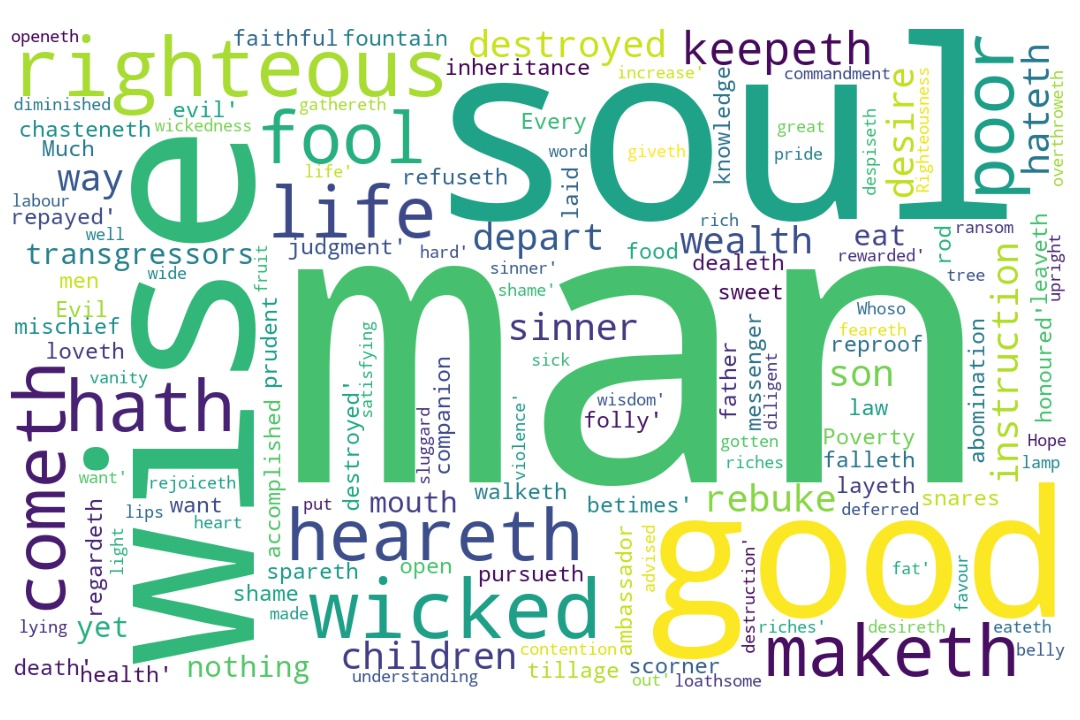
\includegraphics[width=\linewidth]{20OT-Proverbs/Proverb13-WordCloud.jpg}
  \caption{Proverb 13 Word Cloud}
  \label{fig:Proverb 13 Word Cloud}
\end{figure}

\marginpar{\scriptsize \centering \fcolorbox{bone}{lime}{\textbf{A WISE MAN}}\\ (Proverbs 13:1-25) \begin{compactenum}[I.][8]
    \item \textbf{Hears Instruction} \index[scripture]{Proverbs!Pro 13:01}(Pro 13:1)
    \item \textbf{Holds His Tongue} \index[scripture]{Proverbs!Pro 13:03}(Pro 13:3)
    \item \textbf{Hates Lying} \index[scripture]{Proverbs!Pro 13:05}(Pro 13:5)
    \item Is \textbf{Held up by Righteousness} \index[scripture]{Proverbs!Pro 13:06}(Pro 13:6)
    \item \textbf{Has True Wealth} \index[scripture]{Proverbs!Pro 13:07}(Pro 13:7)
    \item \textbf{Hearkens to God's Word} \index[scripture]{Proverbs!Pro 13:13}(Pro 13:13)
    \item \textbf{Hangs out with other wise Men} \index[scripture]{Proverbs!Pro 13:20}(Pro 13:20)
\end{compactenum}}

\marginpar{\scriptsize \centering \fcolorbox{bone}{yellow}{\textbf{A WISE SON}}\\ (Proverbs 13:1-25) \begin{compactenum}[I.][8]
    \item \textbf{Listens} to Instruction \index[scripture]{Proverbs!Pro 13:01}(Pro 13:1)
    \item \textbf{Learns}  \index[scripture]{Proverbs!Pro 13:01}(Pro 13:1)
    \item \textbf{Locks} his Lips \index[scripture]{Proverbs!Pro 13:03}(Pro 13:3)
    \item \textbf{Labours}  \index[scripture]{Proverbs!Pro 13:11}(Pro 13:11)
    \item \textbf{Likes} Reproof \index[scripture]{Proverbs!Pro 13:18}(Pro 13:18)
    \item \textbf{Leaves} an Inheritance \index[scripture]{Proverbs!Pro 13:22}(Pro 13:22)
    \item \textbf{Loves} Enough to Correct \index[scripture]{Proverbs!Pro 13:24}(Pro 13:24)
\end{compactenum}}

\footnote{\textcolor[cmyk]{0.99998,1,0,0}{\hyperlink{TOC}{Return to end of Table of Contents.}}}\footnote{\href{https://audiobible.com/bible/proverbs_13.html}{\textcolor[cmyk]{0.99998,1,0,0}{Proverbs Audio}}}\textcolor[cmyk]{0.99998,1,0,0}{A wise son \fcolorbox{bone}{lime}{\emph{heareth} his father's instruction}: but a scorner heareth not rebuke.}\footnote{\textbf{Isaiah 29:20} - For the terrible one is brought to nought, and the scorner is consumed, and all that watch for iniquity are cut off:}
[2] \textcolor[cmyk]{0.99998,1,0,0}{A man \fcolorbox{bone}{bone}{shall} eat good by the fruit of \emph{his} mouth: but the soul of the \fcolorbox{bone}{MYGOLD}{transgressors} \emph{\fcolorbox{bone}{bone}{shall}} \emph{eat} violence.}
[3] \textcolor[cmyk]{0.99998,1,0,0}{He that \fcolorbox{bone}{lime}{keepeth his mouth} keepeth his life: \emph{but} he that openeth wide his lips \fcolorbox{bone}{bone}{shall} have destruction.}
[4] \textcolor[cmyk]{0.99998,1,0,0}{The soul of the sluggard desireth, and \emph{hath} nothing: but the soul of the diligent \fcolorbox{bone}{bone}{shall} be made fat.}
[5] \textcolor[cmyk]{0.99998,1,0,0}{A righteous \emph{man} \fcolorbox{bone}{lime}{hateth lying}: but a wicked \emph{man} is loathsome, and cometh to shame.}
[6] \textcolor[cmyk]{0.99998,1,0,0}{\fcolorbox{bone}{MYGOLD}{Righteousness} keepeth \emph{him} \emph{that} \emph{is} upright in the way: but wickedness overthroweth the sinner.}
[7] \textcolor[cmyk]{0.99998,1,0,0}{There is that maketh himself rich, yet \emph{hath} nothing: \emph{there} \emph{is} that maketh himself poor, \fcolorbox{bone}{lime}{yet \emph{hath} great riches}.}
[8] \textcolor[cmyk]{0.99998,1,0,0}{The ransom of a man's life \emph{are} his riches: but the poor heareth not rebuke.}
[9] \textcolor[cmyk]{0.99998,1,0,0}{The light of the righteous rejoiceth: but the lamp of the wicked \fcolorbox{bone}{bone}{shall} be put out.}
[10] \textcolor[cmyk]{0.99998,1,0,0}{Only by pride cometh contention: but with the well advised \emph{is} wisdom.}
[11] \textcolor[cmyk]{0.99998,1,0,0}{Wealth \emph{gotten} by vanity \fcolorbox{bone}{bone}{shall} be diminished: but he that gathereth by labour \fcolorbox{bone}{bone}{shall} increase.}
[12] \textcolor[cmyk]{0.99998,1,0,0}{Hope deferred maketh the heart sick: but \emph{when} the desire cometh, \emph{it} \emph{is} a tree of life.}
[13] \textcolor[cmyk]{0.99998,1,0,0}{Whoso despiseth the word \fcolorbox{bone}{bone}{shall} be destroyed: but he that \fcolorbox{bone}{lime}{feareth the commandment} \fcolorbox{bone}{bone}{shall} be rewarded.}
[14] \textcolor[cmyk]{0.99998,1,0,0}{The law of the wise \emph{is} a fountain of life, to depart from the snares of death.}
[15] \textcolor[cmyk]{0.99998,1,0,0}{Good \fcolorbox{bone}{MYGOLD}{understanding} giveth favour: but the way of \fcolorbox{bone}{MYGOLD}{transgressors} \emph{is} hard.}
[16] \textcolor[cmyk]{0.99998,1,0,0}{Every prudent \emph{man} dealeth with knowledge: but a fool layeth open \emph{his} folly.}
[17] \textcolor[cmyk]{0.99998,1,0,0}{A wicked messenger falleth into mischief: but a faithful ambassador \emph{is} health.}
[18] \textcolor[cmyk]{0.99998,1,0,0}{Poverty and shame \emph{\fcolorbox{bone}{bone}{shall}} \emph{be} \emph{to} him that refuseth instruction: but he that regardeth reproof \fcolorbox{bone}{bone}{shall} be honoured.}
[19] \textcolor[cmyk]{0.99998,1,0,0}{The desire accomplished is sweet to the soul: but \emph{it} \emph{is} abomination to fools to depart from evil.}
[20] \textcolor[cmyk]{0.99998,1,0,0}{He that \fcolorbox{bone}{lime}{walketh with wise \emph{men}} \fcolorbox{bone}{bone}{shall} be wise: but a companion of fools \fcolorbox{bone}{bone}{shall} be destroyed.}\footnote{\textbf{2 Kings 9:11} - Then Jehu came forth to the servants of his lord: and one said unto him, Is all well? wherefore came this mad fellow to thee? And he said unto them, Ye know the man, and his communication.}\footnote{\textbf{1 Corinthians 15:33} - Be not deceived: evil communications corrupt good manners.}
[21] \textcolor[cmyk]{0.99998,1,0,0}{Evil pursueth sinners: but to the righteous good \fcolorbox{bone}{bone}{shall} be repayed.}
[22] \textcolor[cmyk]{0.99998,1,0,0}{A good \emph{man} leaveth an inheritance to his children's children: and the wealth of the sinner \emph{is} laid up for the just.}
[23] \textcolor[cmyk]{0.99998,1,0,0}{Much food \emph{is} \emph{in} the tillage of the poor: but there is \emph{that} \emph{is} destroyed for want of judgment.}
[24] \textcolor[cmyk]{0.99998,1,0,0}{He that spareth his rod hateth his son: but he that loveth him chasteneth him betimes.}
[25] \textcolor[cmyk]{0.99998,1,0,0}{The righteous eateth to the satisfying of his soul: but the belly of the wicked \fcolorbox{bone}{bone}{shall} want.}


% ransom , rebuke, refuseth, regardeth, rejoiceth, repayed, reproof, rewarded, rich, riches, righteous, rod

\index[NWIV]{13!Proverbs!Pro 13:1}\index[AWIP]{A!Proverbs!Pro 13:1}\index[AWIP]{wise!Proverbs!Pro 13:1}\index[AWIP]{son!Proverbs!Pro 13:1}\index[AWIP]{\emph{heareth}!Proverbs!Pro 13:1}\index[AWIP]{his!Proverbs!Pro 13:1}\index[AWIP]{father's!Proverbs!Pro 13:1}\index[AWIP]{instruction!Proverbs!Pro 13:1}\index[AWIP]{but!Proverbs!Pro 13:1}\index[AWIP]{a!Proverbs!Pro 13:1}\index[AWIP]{scorner!Proverbs!Pro 13:1}\index[AWIP]{heareth!Proverbs!Pro 13:1}\index[AWIP]{not!Proverbs!Pro 13:1}\index[AWIP]{rebuke!Proverbs!Pro 13:1}\index[AWIP]{\emph{heareth}!Proverbs!Pro 13:1}

\index[NWIV]{20!Proverbs!Pro 13:2}\index[AWIP]{A!Proverbs!Pro 13:2}\index[AWIP]{man!Proverbs!Pro 13:2}\index[AWIP]{shall!Proverbs!Pro 13:2}\index[AWIP]{eat!Proverbs!Pro 13:2}\index[AWIP]{good!Proverbs!Pro 13:2}\index[AWIP]{by!Proverbs!Pro 13:2}\index[AWIP]{the!Proverbs!Pro 13:2}\index[AWIP]{the!Proverbs!Pro 13:2 (2)}\index[AWIP]{the!Proverbs!Pro 13:2 (3)}\index[AWIP]{fruit!Proverbs!Pro 13:2}\index[AWIP]{of!Proverbs!Pro 13:2}\index[AWIP]{of!Proverbs!Pro 13:2 (2)}\index[AWIP]{\emph{his}!Proverbs!Pro 13:2}\index[AWIP]{mouth!Proverbs!Pro 13:2}\index[AWIP]{but!Proverbs!Pro 13:2}\index[AWIP]{soul!Proverbs!Pro 13:2}\index[AWIP]{transgressors!Proverbs!Pro 13:2}\index[AWIP]{\emph{shall}!Proverbs!Pro 13:2}\index[AWIP]{\emph{eat}!Proverbs!Pro 13:2}\index[AWIP]{violence!Proverbs!Pro 13:2}\index[AWIP]{\emph{his}!Proverbs!Pro 13:2}\index[AWIP]{\emph{shall}!Proverbs!Pro 13:2}\index[AWIP]{\emph{eat}!Proverbs!Pro 13:2}

\index[NWIV]{18!Proverbs!Pro 13:3}\index[AWIP]{He!Proverbs!Pro 13:3}\index[AWIP]{that!Proverbs!Pro 13:3}\index[AWIP]{that!Proverbs!Pro 13:3 (2)}\index[AWIP]{keepeth!Proverbs!Pro 13:3}\index[AWIP]{keepeth!Proverbs!Pro 13:3 (2)}\index[AWIP]{his!Proverbs!Pro 13:3}\index[AWIP]{his!Proverbs!Pro 13:3 (2)}\index[AWIP]{his!Proverbs!Pro 13:3 (3)}\index[AWIP]{mouth!Proverbs!Pro 13:3}\index[AWIP]{life!Proverbs!Pro 13:3}\index[AWIP]{\emph{but}!Proverbs!Pro 13:3}\index[AWIP]{he!Proverbs!Pro 13:3}\index[AWIP]{openeth!Proverbs!Pro 13:3}\index[AWIP]{wide!Proverbs!Pro 13:3}\index[AWIP]{lips!Proverbs!Pro 13:3}\index[AWIP]{shall!Proverbs!Pro 13:3}\index[AWIP]{have!Proverbs!Pro 13:3}\index[AWIP]{destruction!Proverbs!Pro 13:3}\index[AWIP]{\emph{but}!Proverbs!Pro 13:3}

\index[NWIV]{19!Proverbs!Pro 13:4}\index[AWIP]{The!Proverbs!Pro 13:4}\index[AWIP]{soul!Proverbs!Pro 13:4}\index[AWIP]{soul!Proverbs!Pro 13:4 (2)}\index[AWIP]{of!Proverbs!Pro 13:4}\index[AWIP]{of!Proverbs!Pro 13:4 (2)}\index[AWIP]{the!Proverbs!Pro 13:4}\index[AWIP]{the!Proverbs!Pro 13:4 (2)}\index[AWIP]{the!Proverbs!Pro 13:4 (3)}\index[AWIP]{sluggard!Proverbs!Pro 13:4}\index[AWIP]{desireth!Proverbs!Pro 13:4}\index[AWIP]{and!Proverbs!Pro 13:4}\index[AWIP]{\emph{hath}!Proverbs!Pro 13:4}\index[AWIP]{nothing!Proverbs!Pro 13:4}\index[AWIP]{but!Proverbs!Pro 13:4}\index[AWIP]{diligent!Proverbs!Pro 13:4}\index[AWIP]{shall!Proverbs!Pro 13:4}\index[AWIP]{be!Proverbs!Pro 13:4}\index[AWIP]{made!Proverbs!Pro 13:4}\index[AWIP]{fat!Proverbs!Pro 13:4}\index[AWIP]{\emph{hath}!Proverbs!Pro 13:4}

\index[NWIV]{15!Proverbs!Pro 13:5}\index[AWIP]{A!Proverbs!Pro 13:5}\index[AWIP]{righteous!Proverbs!Pro 13:5}\index[AWIP]{\emph{man}!Proverbs!Pro 13:5}\index[AWIP]{\emph{man}!Proverbs!Pro 13:5 (2)}\index[AWIP]{hateth!Proverbs!Pro 13:5}\index[AWIP]{lying!Proverbs!Pro 13:5}\index[AWIP]{but!Proverbs!Pro 13:5}\index[AWIP]{a!Proverbs!Pro 13:5}\index[AWIP]{wicked!Proverbs!Pro 13:5}\index[AWIP]{is!Proverbs!Pro 13:5}\index[AWIP]{loathsome!Proverbs!Pro 13:5}\index[AWIP]{and!Proverbs!Pro 13:5}\index[AWIP]{cometh!Proverbs!Pro 13:5}\index[AWIP]{to!Proverbs!Pro 13:5}\index[AWIP]{shame!Proverbs!Pro 13:5}\index[AWIP]{\emph{man}!Proverbs!Pro 13:5}\index[AWIP]{\emph{man}!Proverbs!Pro 13:5 (2)}

\index[NWIV]{14!Proverbs!Pro 13:6}\index[AWIP]{Righteousness!Proverbs!Pro 13:6}\index[AWIP]{keepeth!Proverbs!Pro 13:6}\index[AWIP]{\emph{him}!Proverbs!Pro 13:6}\index[AWIP]{\emph{that}!Proverbs!Pro 13:6}\index[AWIP]{\emph{is}!Proverbs!Pro 13:6}\index[AWIP]{upright!Proverbs!Pro 13:6}\index[AWIP]{in!Proverbs!Pro 13:6}\index[AWIP]{the!Proverbs!Pro 13:6}\index[AWIP]{the!Proverbs!Pro 13:6 (2)}\index[AWIP]{way!Proverbs!Pro 13:6}\index[AWIP]{but!Proverbs!Pro 13:6}\index[AWIP]{wickedness!Proverbs!Pro 13:6}\index[AWIP]{overthroweth!Proverbs!Pro 13:6}\index[AWIP]{sinner!Proverbs!Pro 13:6}\index[AWIP]{\emph{him}!Proverbs!Pro 13:6}\index[AWIP]{\emph{that}!Proverbs!Pro 13:6}\index[AWIP]{\emph{is}!Proverbs!Pro 13:6}

\index[NWIV]{19!Proverbs!Pro 13:7}\index[AWIP]{There!Proverbs!Pro 13:7}\index[AWIP]{is!Proverbs!Pro 13:7}\index[AWIP]{that!Proverbs!Pro 13:7}\index[AWIP]{that!Proverbs!Pro 13:7 (2)}\index[AWIP]{maketh!Proverbs!Pro 13:7}\index[AWIP]{maketh!Proverbs!Pro 13:7 (2)}\index[AWIP]{himself!Proverbs!Pro 13:7}\index[AWIP]{himself!Proverbs!Pro 13:7 (2)}\index[AWIP]{rich!Proverbs!Pro 13:7}\index[AWIP]{yet!Proverbs!Pro 13:7}\index[AWIP]{yet!Proverbs!Pro 13:7 (2)}\index[AWIP]{\emph{hath}!Proverbs!Pro 13:7}\index[AWIP]{\emph{hath}!Proverbs!Pro 13:7 (2)}\index[AWIP]{nothing!Proverbs!Pro 13:7}\index[AWIP]{\emph{there}!Proverbs!Pro 13:7}\index[AWIP]{\emph{is}!Proverbs!Pro 13:7}\index[AWIP]{poor!Proverbs!Pro 13:7}\index[AWIP]{great!Proverbs!Pro 13:7}\index[AWIP]{riches!Proverbs!Pro 13:7}\index[AWIP]{\emph{hath}!Proverbs!Pro 13:7}\index[AWIP]{\emph{hath}!Proverbs!Pro 13:7 (2)}\index[AWIP]{\emph{there}!Proverbs!Pro 13:7}\index[AWIP]{\emph{is}!Proverbs!Pro 13:7}

\index[NWIV]{15!Proverbs!Pro 13:8}\index[AWIP]{The!Proverbs!Pro 13:8}\index[AWIP]{ransom!Proverbs!Pro 13:8}\index[AWIP]{of!Proverbs!Pro 13:8}\index[AWIP]{a!Proverbs!Pro 13:8}\index[AWIP]{man's!Proverbs!Pro 13:8}\index[AWIP]{life!Proverbs!Pro 13:8}\index[AWIP]{\emph{are}!Proverbs!Pro 13:8}\index[AWIP]{his!Proverbs!Pro 13:8}\index[AWIP]{riches!Proverbs!Pro 13:8}\index[AWIP]{but!Proverbs!Pro 13:8}\index[AWIP]{the!Proverbs!Pro 13:8}\index[AWIP]{poor!Proverbs!Pro 13:8}\index[AWIP]{heareth!Proverbs!Pro 13:8}\index[AWIP]{not!Proverbs!Pro 13:8}\index[AWIP]{rebuke!Proverbs!Pro 13:8}\index[AWIP]{\emph{are}!Proverbs!Pro 13:8}

\index[NWIV]{16!Proverbs!Pro 13:9}\index[AWIP]{The!Proverbs!Pro 13:9}\index[AWIP]{light!Proverbs!Pro 13:9}\index[AWIP]{of!Proverbs!Pro 13:9}\index[AWIP]{of!Proverbs!Pro 13:9 (2)}\index[AWIP]{the!Proverbs!Pro 13:9}\index[AWIP]{the!Proverbs!Pro 13:9 (2)}\index[AWIP]{the!Proverbs!Pro 13:9 (3)}\index[AWIP]{righteous!Proverbs!Pro 13:9}\index[AWIP]{rejoiceth!Proverbs!Pro 13:9}\index[AWIP]{but!Proverbs!Pro 13:9}\index[AWIP]{lamp!Proverbs!Pro 13:9}\index[AWIP]{wicked!Proverbs!Pro 13:9}\index[AWIP]{shall!Proverbs!Pro 13:9}\index[AWIP]{be!Proverbs!Pro 13:9}\index[AWIP]{put!Proverbs!Pro 13:9}\index[AWIP]{out!Proverbs!Pro 13:9}

\index[NWIV]{12!Proverbs!Pro 13:10}\index[AWIP]{Only!Proverbs!Pro 13:10}\index[AWIP]{by!Proverbs!Pro 13:10}\index[AWIP]{pride!Proverbs!Pro 13:10}\index[AWIP]{cometh!Proverbs!Pro 13:10}\index[AWIP]{contention!Proverbs!Pro 13:10}\index[AWIP]{but!Proverbs!Pro 13:10}\index[AWIP]{with!Proverbs!Pro 13:10}\index[AWIP]{the!Proverbs!Pro 13:10}\index[AWIP]{well!Proverbs!Pro 13:10}\index[AWIP]{advised!Proverbs!Pro 13:10}\index[AWIP]{\emph{is}!Proverbs!Pro 13:10}\index[AWIP]{wisdom!Proverbs!Pro 13:10}\index[AWIP]{\emph{is}!Proverbs!Pro 13:10}

\index[NWIV]{15!Proverbs!Pro 13:11}\index[AWIP]{Wealth!Proverbs!Pro 13:11}\index[AWIP]{\emph{gotten}!Proverbs!Pro 13:11}\index[AWIP]{by!Proverbs!Pro 13:11}\index[AWIP]{by!Proverbs!Pro 13:11 (2)}\index[AWIP]{vanity!Proverbs!Pro 13:11}\index[AWIP]{shall!Proverbs!Pro 13:11}\index[AWIP]{shall!Proverbs!Pro 13:11 (2)}\index[AWIP]{be!Proverbs!Pro 13:11}\index[AWIP]{diminished!Proverbs!Pro 13:11}\index[AWIP]{but!Proverbs!Pro 13:11}\index[AWIP]{he!Proverbs!Pro 13:11}\index[AWIP]{that!Proverbs!Pro 13:11}\index[AWIP]{gathereth!Proverbs!Pro 13:11}\index[AWIP]{labour!Proverbs!Pro 13:11}\index[AWIP]{increase!Proverbs!Pro 13:11}\index[AWIP]{\emph{gotten}!Proverbs!Pro 13:11}

\index[NWIV]{17!Proverbs!Pro 13:12}\index[AWIP]{Hope!Proverbs!Pro 13:12}\index[AWIP]{deferred!Proverbs!Pro 13:12}\index[AWIP]{maketh!Proverbs!Pro 13:12}\index[AWIP]{the!Proverbs!Pro 13:12}\index[AWIP]{the!Proverbs!Pro 13:12 (2)}\index[AWIP]{heart!Proverbs!Pro 13:12}\index[AWIP]{sick!Proverbs!Pro 13:12}\index[AWIP]{but!Proverbs!Pro 13:12}\index[AWIP]{\emph{when}!Proverbs!Pro 13:12}\index[AWIP]{desire!Proverbs!Pro 13:12}\index[AWIP]{cometh!Proverbs!Pro 13:12}\index[AWIP]{\emph{it}!Proverbs!Pro 13:12}\index[AWIP]{\emph{is}!Proverbs!Pro 13:12}\index[AWIP]{a!Proverbs!Pro 13:12}\index[AWIP]{tree!Proverbs!Pro 13:12}\index[AWIP]{of!Proverbs!Pro 13:12}\index[AWIP]{life!Proverbs!Pro 13:12}\index[AWIP]{\emph{when}!Proverbs!Pro 13:12}\index[AWIP]{\emph{it}!Proverbs!Pro 13:12}\index[AWIP]{\emph{is}!Proverbs!Pro 13:12}

\index[NWIV]{16!Proverbs!Pro 13:13}\index[AWIP]{Whoso!Proverbs!Pro 13:13}\index[AWIP]{despiseth!Proverbs!Pro 13:13}\index[AWIP]{the!Proverbs!Pro 13:13}\index[AWIP]{the!Proverbs!Pro 13:13 (2)}\index[AWIP]{word!Proverbs!Pro 13:13}\index[AWIP]{shall!Proverbs!Pro 13:13}\index[AWIP]{shall!Proverbs!Pro 13:13 (2)}\index[AWIP]{be!Proverbs!Pro 13:13}\index[AWIP]{be!Proverbs!Pro 13:13 (2)}\index[AWIP]{destroyed!Proverbs!Pro 13:13}\index[AWIP]{but!Proverbs!Pro 13:13}\index[AWIP]{he!Proverbs!Pro 13:13}\index[AWIP]{that!Proverbs!Pro 13:13}\index[AWIP]{feareth!Proverbs!Pro 13:13}\index[AWIP]{commandment!Proverbs!Pro 13:13}\index[AWIP]{rewarded!Proverbs!Pro 13:13}

\index[NWIV]{17!Proverbs!Pro 13:14}\index[AWIP]{The!Proverbs!Pro 13:14}\index[AWIP]{law!Proverbs!Pro 13:14}\index[AWIP]{of!Proverbs!Pro 13:14}\index[AWIP]{of!Proverbs!Pro 13:14 (2)}\index[AWIP]{of!Proverbs!Pro 13:14 (3)}\index[AWIP]{the!Proverbs!Pro 13:14}\index[AWIP]{the!Proverbs!Pro 13:14 (2)}\index[AWIP]{wise!Proverbs!Pro 13:14}\index[AWIP]{\emph{is}!Proverbs!Pro 13:14}\index[AWIP]{a!Proverbs!Pro 13:14}\index[AWIP]{fountain!Proverbs!Pro 13:14}\index[AWIP]{life!Proverbs!Pro 13:14}\index[AWIP]{to!Proverbs!Pro 13:14}\index[AWIP]{depart!Proverbs!Pro 13:14}\index[AWIP]{from!Proverbs!Pro 13:14}\index[AWIP]{snares!Proverbs!Pro 13:14}\index[AWIP]{death!Proverbs!Pro 13:14}\index[AWIP]{\emph{is}!Proverbs!Pro 13:14}

\index[NWIV]{11!Proverbs!Pro 13:15}\index[AWIP]{Good!Proverbs!Pro 13:15}\index[AWIP]{understanding!Proverbs!Pro 13:15}\index[AWIP]{giveth!Proverbs!Pro 13:15}\index[AWIP]{favour!Proverbs!Pro 13:15}\index[AWIP]{but!Proverbs!Pro 13:15}\index[AWIP]{the!Proverbs!Pro 13:15}\index[AWIP]{way!Proverbs!Pro 13:15}\index[AWIP]{of!Proverbs!Pro 13:15}\index[AWIP]{transgressors!Proverbs!Pro 13:15}\index[AWIP]{\emph{is}!Proverbs!Pro 13:15}\index[AWIP]{hard!Proverbs!Pro 13:15}\index[AWIP]{\emph{is}!Proverbs!Pro 13:15}

\index[NWIV]{13!Proverbs!Pro 13:16}\index[AWIP]{Every!Proverbs!Pro 13:16}\index[AWIP]{prudent!Proverbs!Pro 13:16}\index[AWIP]{\emph{man}!Proverbs!Pro 13:16}\index[AWIP]{dealeth!Proverbs!Pro 13:16}\index[AWIP]{with!Proverbs!Pro 13:16}\index[AWIP]{knowledge!Proverbs!Pro 13:16}\index[AWIP]{but!Proverbs!Pro 13:16}\index[AWIP]{a!Proverbs!Pro 13:16}\index[AWIP]{fool!Proverbs!Pro 13:16}\index[AWIP]{layeth!Proverbs!Pro 13:16}\index[AWIP]{open!Proverbs!Pro 13:16}\index[AWIP]{\emph{his}!Proverbs!Pro 13:16}\index[AWIP]{folly!Proverbs!Pro 13:16}\index[AWIP]{\emph{man}!Proverbs!Pro 13:16}\index[AWIP]{\emph{his}!Proverbs!Pro 13:16}

\index[NWIV]{12!Proverbs!Pro 13:17}\index[AWIP]{A!Proverbs!Pro 13:17}\index[AWIP]{wicked!Proverbs!Pro 13:17}\index[AWIP]{messenger!Proverbs!Pro 13:17}\index[AWIP]{falleth!Proverbs!Pro 13:17}\index[AWIP]{into!Proverbs!Pro 13:17}\index[AWIP]{mischief!Proverbs!Pro 13:17}\index[AWIP]{but!Proverbs!Pro 13:17}\index[AWIP]{a!Proverbs!Pro 13:17}\index[AWIP]{faithful!Proverbs!Pro 13:17}\index[AWIP]{ambassador!Proverbs!Pro 13:17}\index[AWIP]{\emph{is}!Proverbs!Pro 13:17}\index[AWIP]{health!Proverbs!Pro 13:17}\index[AWIP]{\emph{is}!Proverbs!Pro 13:17}

\index[NWIV]{18!Proverbs!Pro 13:18}\index[AWIP]{Poverty!Proverbs!Pro 13:18}\index[AWIP]{and!Proverbs!Pro 13:18}\index[AWIP]{shame!Proverbs!Pro 13:18}\index[AWIP]{\emph{shall}!Proverbs!Pro 13:18}\index[AWIP]{\emph{be}!Proverbs!Pro 13:18}\index[AWIP]{\emph{to}!Proverbs!Pro 13:18}\index[AWIP]{him!Proverbs!Pro 13:18}\index[AWIP]{that!Proverbs!Pro 13:18}\index[AWIP]{that!Proverbs!Pro 13:18 (2)}\index[AWIP]{refuseth!Proverbs!Pro 13:18}\index[AWIP]{instruction!Proverbs!Pro 13:18}\index[AWIP]{but!Proverbs!Pro 13:18}\index[AWIP]{he!Proverbs!Pro 13:18}\index[AWIP]{regardeth!Proverbs!Pro 13:18}\index[AWIP]{reproof!Proverbs!Pro 13:18}\index[AWIP]{shall!Proverbs!Pro 13:18}\index[AWIP]{be!Proverbs!Pro 13:18}\index[AWIP]{honoured!Proverbs!Pro 13:18}\index[AWIP]{\emph{shall}!Proverbs!Pro 13:18}\index[AWIP]{\emph{be}!Proverbs!Pro 13:18}\index[AWIP]{\emph{to}!Proverbs!Pro 13:18}

\index[NWIV]{18!Proverbs!Pro 13:19}\index[AWIP]{The!Proverbs!Pro 13:19}\index[AWIP]{desire!Proverbs!Pro 13:19}\index[AWIP]{accomplished!Proverbs!Pro 13:19}\index[AWIP]{is!Proverbs!Pro 13:19}\index[AWIP]{sweet!Proverbs!Pro 13:19}\index[AWIP]{to!Proverbs!Pro 13:19}\index[AWIP]{to!Proverbs!Pro 13:19 (2)}\index[AWIP]{to!Proverbs!Pro 13:19 (3)}\index[AWIP]{the!Proverbs!Pro 13:19}\index[AWIP]{soul!Proverbs!Pro 13:19}\index[AWIP]{but!Proverbs!Pro 13:19}\index[AWIP]{\emph{it}!Proverbs!Pro 13:19}\index[AWIP]{\emph{is}!Proverbs!Pro 13:19}\index[AWIP]{abomination!Proverbs!Pro 13:19}\index[AWIP]{fools!Proverbs!Pro 13:19}\index[AWIP]{depart!Proverbs!Pro 13:19}\index[AWIP]{from!Proverbs!Pro 13:19}\index[AWIP]{evil!Proverbs!Pro 13:19}\index[AWIP]{\emph{it}!Proverbs!Pro 13:19}\index[AWIP]{\emph{is}!Proverbs!Pro 13:19}

\index[NWIV]{17!Proverbs!Pro 13:20}\index[AWIP]{He!Proverbs!Pro 13:20}\index[AWIP]{that!Proverbs!Pro 13:20}\index[AWIP]{walketh!Proverbs!Pro 13:20}\index[AWIP]{with!Proverbs!Pro 13:20}\index[AWIP]{wise!Proverbs!Pro 13:20}\index[AWIP]{wise!Proverbs!Pro 13:20 (2)}\index[AWIP]{\emph{men}!Proverbs!Pro 13:20}\index[AWIP]{shall!Proverbs!Pro 13:20}\index[AWIP]{shall!Proverbs!Pro 13:20 (2)}\index[AWIP]{be!Proverbs!Pro 13:20}\index[AWIP]{be!Proverbs!Pro 13:20 (2)}\index[AWIP]{but!Proverbs!Pro 13:20}\index[AWIP]{a!Proverbs!Pro 13:20}\index[AWIP]{companion!Proverbs!Pro 13:20}\index[AWIP]{of!Proverbs!Pro 13:20}\index[AWIP]{fools!Proverbs!Pro 13:20}\index[AWIP]{destroyed!Proverbs!Pro 13:20}\index[AWIP]{\emph{men}!Proverbs!Pro 13:20}

\index[NWIV]{11!Proverbs!Pro 13:21}\index[AWIP]{Evil!Proverbs!Pro 13:21}\index[AWIP]{pursueth!Proverbs!Pro 13:21}\index[AWIP]{sinners!Proverbs!Pro 13:21}\index[AWIP]{but!Proverbs!Pro 13:21}\index[AWIP]{to!Proverbs!Pro 13:21}\index[AWIP]{the!Proverbs!Pro 13:21}\index[AWIP]{righteous!Proverbs!Pro 13:21}\index[AWIP]{good!Proverbs!Pro 13:21}\index[AWIP]{shall!Proverbs!Pro 13:21}\index[AWIP]{be!Proverbs!Pro 13:21}\index[AWIP]{repayed!Proverbs!Pro 13:21}

\index[NWIV]{22!Proverbs!Pro 13:22}\index[AWIP]{A!Proverbs!Pro 13:22}\index[AWIP]{good!Proverbs!Pro 13:22}\index[AWIP]{\emph{man}!Proverbs!Pro 13:22}\index[AWIP]{leaveth!Proverbs!Pro 13:22}\index[AWIP]{an!Proverbs!Pro 13:22}\index[AWIP]{inheritance!Proverbs!Pro 13:22}\index[AWIP]{to!Proverbs!Pro 13:22}\index[AWIP]{his!Proverbs!Pro 13:22}\index[AWIP]{children's!Proverbs!Pro 13:22}\index[AWIP]{children!Proverbs!Pro 13:22}\index[AWIP]{and!Proverbs!Pro 13:22}\index[AWIP]{the!Proverbs!Pro 13:22}\index[AWIP]{the!Proverbs!Pro 13:22 (2)}\index[AWIP]{the!Proverbs!Pro 13:22 (3)}\index[AWIP]{wealth!Proverbs!Pro 13:22}\index[AWIP]{of!Proverbs!Pro 13:22}\index[AWIP]{sinner!Proverbs!Pro 13:22}\index[AWIP]{\emph{is}!Proverbs!Pro 13:22}\index[AWIP]{laid!Proverbs!Pro 13:22}\index[AWIP]{up!Proverbs!Pro 13:22}\index[AWIP]{for!Proverbs!Pro 13:22}\index[AWIP]{just!Proverbs!Pro 13:22}\index[AWIP]{\emph{man}!Proverbs!Pro 13:22}\index[AWIP]{\emph{is}!Proverbs!Pro 13:22}

\index[NWIV]{19!Proverbs!Pro 13:23}\index[AWIP]{Much!Proverbs!Pro 13:23}\index[AWIP]{food!Proverbs!Pro 13:23}\index[AWIP]{\emph{is}!Proverbs!Pro 13:23}\index[AWIP]{\emph{is}!Proverbs!Pro 13:23 (2)}\index[AWIP]{\emph{in}!Proverbs!Pro 13:23}\index[AWIP]{the!Proverbs!Pro 13:23}\index[AWIP]{the!Proverbs!Pro 13:23 (2)}\index[AWIP]{tillage!Proverbs!Pro 13:23}\index[AWIP]{of!Proverbs!Pro 13:23}\index[AWIP]{of!Proverbs!Pro 13:23 (2)}\index[AWIP]{poor!Proverbs!Pro 13:23}\index[AWIP]{but!Proverbs!Pro 13:23}\index[AWIP]{there!Proverbs!Pro 13:23}\index[AWIP]{is!Proverbs!Pro 13:23}\index[AWIP]{\emph{that}!Proverbs!Pro 13:23}\index[AWIP]{destroyed!Proverbs!Pro 13:23}\index[AWIP]{for!Proverbs!Pro 13:23}\index[AWIP]{want!Proverbs!Pro 13:23}\index[AWIP]{judgment!Proverbs!Pro 13:23}\index[AWIP]{\emph{is}!Proverbs!Pro 13:23}\index[AWIP]{\emph{is}!Proverbs!Pro 13:23 (2)}\index[AWIP]{\emph{in}!Proverbs!Pro 13:23}\index[AWIP]{\emph{that}!Proverbs!Pro 13:23}

\index[NWIV]{16!Proverbs!Pro 13:24}\index[AWIP]{He!Proverbs!Pro 13:24}\index[AWIP]{that!Proverbs!Pro 13:24}\index[AWIP]{that!Proverbs!Pro 13:24 (2)}\index[AWIP]{spareth!Proverbs!Pro 13:24}\index[AWIP]{his!Proverbs!Pro 13:24}\index[AWIP]{his!Proverbs!Pro 13:24 (2)}\index[AWIP]{rod!Proverbs!Pro 13:24}\index[AWIP]{hateth!Proverbs!Pro 13:24}\index[AWIP]{son!Proverbs!Pro 13:24}\index[AWIP]{but!Proverbs!Pro 13:24}\index[AWIP]{he!Proverbs!Pro 13:24}\index[AWIP]{loveth!Proverbs!Pro 13:24}\index[AWIP]{him!Proverbs!Pro 13:24}\index[AWIP]{him!Proverbs!Pro 13:24 (2)}\index[AWIP]{chasteneth!Proverbs!Pro 13:24}\index[AWIP]{betimes!Proverbs!Pro 13:24}

\index[NWIV]{17!Proverbs!Pro 13:25}\index[AWIP]{The!Proverbs!Pro 13:25}\index[AWIP]{righteous!Proverbs!Pro 13:25}\index[AWIP]{eateth!Proverbs!Pro 13:25}\index[AWIP]{to!Proverbs!Pro 13:25}\index[AWIP]{the!Proverbs!Pro 13:25}\index[AWIP]{the!Proverbs!Pro 13:25 (2)}\index[AWIP]{the!Proverbs!Pro 13:25 (3)}\index[AWIP]{satisfying!Proverbs!Pro 13:25}\index[AWIP]{of!Proverbs!Pro 13:25}\index[AWIP]{of!Proverbs!Pro 13:25 (2)}\index[AWIP]{his!Proverbs!Pro 13:25}\index[AWIP]{soul!Proverbs!Pro 13:25}\index[AWIP]{but!Proverbs!Pro 13:25}\index[AWIP]{belly!Proverbs!Pro 13:25}\index[AWIP]{wicked!Proverbs!Pro 13:25}\index[AWIP]{shall!Proverbs!Pro 13:25}\index[AWIP]{want!Proverbs!Pro 13:25}


\section{Proverb 13 Outlines}

\subsection{My Outlines}

\subsubsection{A Wise Man}

\index[speaker]{Keith Anthony!Proverb 13 (A Wise Man)}
\index[series]{Proverbs (Keith Anthony)!Pro 13 (A Wise Man)}
\index[date]{2016/05/13!Proverbs 13 (A Wise Man) (Keith Anthony)}
\begin{compactenum}[I.]
    \item \textbf{Hears Instruction} \index[scripture]{Proverbs!Pro 13:01}(Pro 13:1)
    \item \textbf{Holds His Tongue} \index[scripture]{Proverbs!Pro 13:03}(Pro 13:3)
    \item \textbf{Hates Lying} \index[scripture]{Proverbs!Pro 13:05}(Pro 13:5)
    \item Is \textbf{Help up by Righteousness} \index[scripture]{Proverbs!Pro 13:06}(Pro 13:6)
    \item \textbf{Has True Wealth} \index[scripture]{Proverbs!Pro 13:07}(Pro 13:7)
    \item \textbf{Hearkens to God's Word} \index[scripture]{Proverbs!Pro 13:13}(Pro 13:13)
    \item \textbf{Hangs out with other wise Men} \index[scripture]{Proverbs!Pro 13:20}(Pro 13:20)
\end{compactenum}

\subsubsection{A Wise Son}

\index[speaker]{Keith Anthony!Proverb 13 (A Wise Son)}
\index[series]{Proverbs (Keith Anthony)!Pro 13 (A Wise Son)}
\index[date]{2020/12/13!Proverbs 13 (A Wise Son) (Keith Anthony)}
 \begin{compactenum}[I.][8]
    \item \textbf{Listens} to Instruction \index[scripture]{Proverbs!Pro 13:01}(Pro 13:1)
    \item \textbf{Learns}  \index[scripture]{Proverbs!Pro 13:01}(Pro 13:1)
    \item \textbf{Locks} his Lips \index[scripture]{Proverbs!Pro 13:03}(Pro 13:3)
    \item \textbf{Labours}  \index[scripture]{Proverbs!Pro 13:11}(Pro 13:11)
    \item \textbf{Likes} Reproof \index[scripture]{Proverbs!Pro 13:18}(Pro 13:18)
    \item \textbf{Leaves} an Inheritance \index[scripture]{Proverbs!Pro 13:22}(Pro 13:22)
    \item \textbf{Loves} Enough to Correct \index[scripture]{Proverbs!Pro 13:24}(Pro 13:24)
\end{compactenum}

\subsection{Outlines from Others}

\section{Proverb 13 Comments}

\subsection{Numeric Nuggets}
\textbf{13:} Verses 1 and 16 have 13 words. Verses 1, 6, 9, 11, 13, 16, and 24 have 13 unique words. The word ``shall'' is found 13 times in the chapter.  The 13-letter words ``transgressors,'' ``Righteousness,'' and ``understanding'' are used in the cahpter.


\subsection{Proverb 13 Repeated Phrases}


%%%%%%%%%%
%%%%%%%%%%
\normalsize
 
\begin{center}
\begin{longtable}{|c|c|}
\caption[Proverb 13 Repeated Phrases]{Proverb 13 Repeated Phrases}\label{table:Repeated Phrases Proverb 13} \\
\hline \multicolumn{1}{|c|}{\textbf{Phrase}} & \multicolumn{1}{c|}{\textbf{Frequency}} \\ \hline 
\endfirsthead
 
\multicolumn{2}{c}
{{\bfseries \tablename\ \thetable{} -- continued from previous page}} \\  
\hline \multicolumn{1}{|c|}{\textbf{Phrase}} & \multicolumn{1}{c|}{\textbf{Frequency}} \\ \hline 
\endhead
 
\hline \multicolumn{2}{c}{{ }} \\ \hline
\endfoot 
of the & 9\\ \hline 
shall be & 9\\ \hline 
but the & 6\\ \hline 
but a & 5\\ \hline 
he that & 5\\ \hline 
but he & 4\\ \hline 
but he that & 4\\ \hline 
the soul & 3\\ \hline 
soul of & 3\\ \hline 
soul of the & 3\\ \hline 
He that & 3\\ \hline 
to the & 3\\ \hline 
\end{longtable}
\end{center}



%%%%%%%%%%
%%%%%%%%%%



%\newpage
\section{Proverb 13 Statistics}

%%%%%%%%%%%%%%%%%%%%%%%%%%%
%%%%% Word Statistics
%%%%%%%%%%%%%%%%%%%%%%%%%%

\normalsize
\subsection{Chapter Word Statistics}


%%%%%%%%%%
%%%%%%%%%%
 
\begin{center}
\begin{longtable}{l|c|c|c|c}
\caption[Stats for Proverb 13]{Stats for Proverb 13} \label{table:Stats for Proverb 13} \\ 
\hline \multicolumn{1}{|c|}{\textbf{Verse(s)}} & \multicolumn{1}{|c|}{\textbf{Count}} & \multicolumn{1}{|c|}{\textbf{Unique}} & \multicolumn{1}{|c|}{\textbf{Italics}} & \multicolumn{1}{|c|}{\textbf{Uniq Italic}}  \\ \hline 
\endfirsthead
 
\multicolumn{5}{c}
{{\bfseries \tablename\ \thetable{} -- continued from previous page}} \\  
\hline \multicolumn{1}{|c|}{\textbf{Verse(s)}} & \multicolumn{1}{|c|}{\textbf{Count}} & \multicolumn{1}{|c|}{\textbf{Unique}} & \multicolumn{1}{|c|}{\textbf{Italics}} & \multicolumn{1}{|c|}{\textbf{Uniq Italic}}  \\ \hline 
\endhead
 
\hline \multicolumn{5}{|r|}{{Continued if needed}} \\ \hline
\endfoot 
1 & 13 & 13 & 1 & 1\\ \hline
2 & 20 & 17 & 3 & 3\\ \hline
3 & 18 & 14 & 1 & 1\\ \hline
4 & 19 & 15 & 1 & 1\\ \hline
5 & 15 & 14 & 2 & 1\\ \hline
6 & 14 & 13 & 3 & 3\\ \hline
7 & 19 & 14 & 4 & 3\\ \hline
8 & 15 & 15 & 1 & 1\\ \hline
9 & 16 & 13 & 0 & 0\\ \hline
10 & 12 & 12 & 1 & 1\\ \hline
11 & 15 & 13 & 1 & 1\\ \hline
12 & 17 & 16 & 3 & 3\\ \hline
13 & 16 & 13 & 0 & 0\\ \hline
14 & 17 & 14 & 1 & 1\\ \hline
15 & 11 & 11 & 1 & 1\\ \hline
16 & 13 & 13 & 2 & 2\\ \hline
17 & 12 & 12 & 1 & 1\\ \hline
18 & 18 & 17 & 3 & 3\\ \hline
19 & 18 & 16 & 2 & 2\\ \hline
20 & 17 & 14 & 1 & 1\\ \hline
21 & 11 & 11 & 0 & 0\\ \hline
22 & 22 & 20 & 2 & 2\\ \hline
23 & 19 & 16 & 4 & 3\\ \hline
24 & 16 & 13 & 0 & 0\\ \hline
25 & 17 & 14 & 0 & 0\\ \hline
\hline \hline
Total & 400 & 186 & 38 & 19




\end{longtable}
\end{center}

%%%%%%%%%%
%%%%%%%%%%


\subsection{Words by Frequency}

\begin{center}
\begin{longtable}{l|r}
\caption[Word Frequencies in Proverb 13]{Word Frequencies in Proverb 13} \label{table:WordsIn-Proverb-13} \\ 
\hline \multicolumn{1}{|c|}{\textbf{Word}} & \multicolumn{1}{c|}{\textbf{Frequency}} \\ \hline 
\endfirsthead
  
\multicolumn{2}{c}  
{{\bfseries \tablename\ \thetable{} -- continued from previous page}} \\   
\hline \multicolumn{1}{|c|}{\textbf{Word}} & \multicolumn{1}{c|}{\textbf{Frequency}} \\ \hline   
\endhead  
  
\hline \multicolumn{2}{|r|}{{Continue}} \\ \hline  
\endfoot  
  
\hline \hline  
\endlastfoot  
  
the & 30\\ \hline 
but & 21\\ \hline 
of & 18\\ \hline 
shall & 13\\ \hline 
that & 11\\ \hline 
\emph{is} & 11\\ \hline 
his & 9\\ \hline 
be & 9\\ \hline 
a & 8\\ \hline 
to & 8\\ \hline 
The & 6\\ \hline 
A & 5\\ \hline 
soul & 5\\ \hline 
he & 5\\ \hline 
wise & 4\\ \hline 
by & 4\\ \hline 
life & 4\\ \hline 
and & 4\\ \hline 
righteous & 4\\ \hline 
\emph{man} & 4\\ \hline 
wicked & 4\\ \hline 
is & 4\\ \hline 
good & 3\\ \hline 
He & 3\\ \hline 
keepeth & 3\\ \hline 
\emph{hath} & 3\\ \hline 
cometh & 3\\ \hline 
maketh & 3\\ \hline 
poor & 3\\ \hline 
with & 3\\ \hline 
destroyed & 3\\ \hline 
him & 3\\ \hline 
son & 2\\ \hline 
instruction & 2\\ \hline 
heareth & 2\\ \hline 
not & 2\\ \hline 
rebuke & 2\\ \hline 
\emph{his} & 2\\ \hline 
mouth & 2\\ \hline 
transgressors & 2\\ \hline 
\emph{shall} & 2\\ \hline 
nothing & 2\\ \hline 
hateth & 2\\ \hline 
shame & 2\\ \hline 
\emph{that} & 2\\ \hline 
way & 2\\ \hline 
sinner & 2\\ \hline 
himself & 2\\ \hline 
yet & 2\\ \hline 
riches & 2\\ \hline 
desire & 2\\ \hline 
\emph{it} & 2\\ \hline 
depart & 2\\ \hline 
from & 2\\ \hline 
fools & 2\\ \hline 
for & 2\\ \hline 
want & 2\\ \hline 
\emph{heareth} & 1\\ \hline 
father's & 1\\ \hline 
scorner & 1\\ \hline 
man & 1\\ \hline 
eat & 1\\ \hline 
fruit & 1\\ \hline 
\emph{eat} & 1\\ \hline 
violence & 1\\ \hline 
\emph{but} & 1\\ \hline 
openeth & 1\\ \hline 
wide & 1\\ \hline 
lips & 1\\ \hline 
have & 1\\ \hline 
destruction & 1\\ \hline 
sluggard & 1\\ \hline 
desireth & 1\\ \hline 
diligent & 1\\ \hline 
made & 1\\ \hline 
fat & 1\\ \hline 
lying & 1\\ \hline 
loathsome & 1\\ \hline 
Righteousness & 1\\ \hline 
\emph{him} & 1\\ \hline 
upright & 1\\ \hline 
in & 1\\ \hline 
wickedness & 1\\ \hline 
overthroweth & 1\\ \hline 
There & 1\\ \hline 
rich & 1\\ \hline 
\emph{there} & 1\\ \hline 
great & 1\\ \hline 
ransom & 1\\ \hline 
man's & 1\\ \hline 
\emph{are} & 1\\ \hline 
light & 1\\ \hline 
rejoiceth & 1\\ \hline 
lamp & 1\\ \hline 
put & 1\\ \hline 
out & 1\\ \hline 
Only & 1\\ \hline 
pride & 1\\ \hline 
contention & 1\\ \hline 
well & 1\\ \hline 
advised & 1\\ \hline 
wisdom & 1\\ \hline 
Wealth & 1\\ \hline 
\emph{gotten} & 1\\ \hline 
vanity & 1\\ \hline 
diminished & 1\\ \hline 
gathereth & 1\\ \hline 
labour & 1\\ \hline 
increase & 1\\ \hline 
Hope & 1\\ \hline 
deferred & 1\\ \hline 
heart & 1\\ \hline 
sick & 1\\ \hline 
\emph{when} & 1\\ \hline 
tree & 1\\ \hline 
Whoso & 1\\ \hline 
despiseth & 1\\ \hline 
word & 1\\ \hline 
feareth & 1\\ \hline 
commandment & 1\\ \hline 
rewarded & 1\\ \hline 
law & 1\\ \hline 
fountain & 1\\ \hline 
snares & 1\\ \hline 
death & 1\\ \hline 
Good & 1\\ \hline 
understanding & 1\\ \hline 
giveth & 1\\ \hline 
favour & 1\\ \hline 
hard & 1\\ \hline 
Every & 1\\ \hline 
prudent & 1\\ \hline 
dealeth & 1\\ \hline 
knowledge & 1\\ \hline 
fool & 1\\ \hline 
layeth & 1\\ \hline 
open & 1\\ \hline 
folly & 1\\ \hline 
messenger & 1\\ \hline 
falleth & 1\\ \hline 
into & 1\\ \hline 
mischief & 1\\ \hline 
faithful & 1\\ \hline 
ambassador & 1\\ \hline 
health & 1\\ \hline 
Poverty & 1\\ \hline 
\emph{be} & 1\\ \hline 
\emph{to} & 1\\ \hline 
refuseth & 1\\ \hline 
regardeth & 1\\ \hline 
reproof & 1\\ \hline 
honoured & 1\\ \hline 
accomplished & 1\\ \hline 
sweet & 1\\ \hline 
abomination & 1\\ \hline 
evil & 1\\ \hline 
walketh & 1\\ \hline 
\emph{men} & 1\\ \hline 
companion & 1\\ \hline 
Evil & 1\\ \hline 
pursueth & 1\\ \hline 
sinners & 1\\ \hline 
repayed & 1\\ \hline 
leaveth & 1\\ \hline 
an & 1\\ \hline 
inheritance & 1\\ \hline 
children's & 1\\ \hline 
children & 1\\ \hline 
wealth & 1\\ \hline 
laid & 1\\ \hline 
up & 1\\ \hline 
just & 1\\ \hline 
Much & 1\\ \hline 
food & 1\\ \hline 
\emph{in} & 1\\ \hline 
tillage & 1\\ \hline 
there & 1\\ \hline 
judgment & 1\\ \hline 
spareth & 1\\ \hline 
rod & 1\\ \hline 
loveth & 1\\ \hline 
chasteneth & 1\\ \hline 
betimes & 1\\ \hline 
eateth & 1\\ \hline 
satisfying & 1\\ \hline 
belly & 1\\ \hline 
\end{longtable}  
\end{center}  


  
\normalsize  

  
  


\subsection{Words Alphabetically}

\begin{center}
\begin{longtable}{l|r}
\caption[Word Frequencies in Proverb 13]{Word Frequencies in Proverb 13} \label{table:WordsIn-Proverb-13} \\ 
\hline \multicolumn{1}{|c|}{\textbf{Word}} & \multicolumn{1}{c|}{\textbf{Frequency}} \\ \hline 
\endfirsthead
  
\multicolumn{2}{c}  
{{\bfseries \tablename\ \thetable{} -- continued from previous page}} \\   
\hline \multicolumn{1}{|c|}{\textbf{Word}} & \multicolumn{1}{c|}{\textbf{Frequency}} \\ \hline   
\endhead  
  
\hline \multicolumn{2}{|r|}{{Continue}} \\ \hline  
\endfoot  
  
\hline \hline  
\endlastfoot  
  
A & 5\\ \hline 
Every & 1\\ \hline 
Evil & 1\\ \hline 
Good & 1\\ \hline 
He & 3\\ \hline 
Hope & 1\\ \hline 
Much & 1\\ \hline 
Only & 1\\ \hline 
Poverty & 1\\ \hline 
Righteousness & 1\\ \hline 
The & 6\\ \hline 
There & 1\\ \hline 
Wealth & 1\\ \hline 
Whoso & 1\\ \hline 
\emph{are} & 1\\ \hline 
\emph{be} & 1\\ \hline 
\emph{but} & 1\\ \hline 
\emph{eat} & 1\\ \hline 
\emph{gotten} & 1\\ \hline 
\emph{hath} & 3\\ \hline 
\emph{heareth} & 1\\ \hline 
\emph{him} & 1\\ \hline 
\emph{his} & 2\\ \hline 
\emph{in} & 1\\ \hline 
\emph{is} & 11\\ \hline 
\emph{it} & 2\\ \hline 
\emph{man} & 4\\ \hline 
\emph{men} & 1\\ \hline 
\emph{shall} & 2\\ \hline 
\emph{that} & 2\\ \hline 
\emph{there} & 1\\ \hline 
\emph{to} & 1\\ \hline 
\emph{when} & 1\\ \hline 
a & 8\\ \hline 
abomination & 1\\ \hline 
accomplished & 1\\ \hline 
advised & 1\\ \hline 
ambassador & 1\\ \hline 
an & 1\\ \hline 
and & 4\\ \hline 
be & 9\\ \hline 
belly & 1\\ \hline 
betimes & 1\\ \hline 
but & 21\\ \hline 
by & 4\\ \hline 
chasteneth & 1\\ \hline 
children & 1\\ \hline 
children's & 1\\ \hline 
cometh & 3\\ \hline 
commandment & 1\\ \hline 
companion & 1\\ \hline 
contention & 1\\ \hline 
dealeth & 1\\ \hline 
death & 1\\ \hline 
deferred & 1\\ \hline 
depart & 2\\ \hline 
desire & 2\\ \hline 
desireth & 1\\ \hline 
despiseth & 1\\ \hline 
destroyed & 3\\ \hline 
destruction & 1\\ \hline 
diligent & 1\\ \hline 
diminished & 1\\ \hline 
eat & 1\\ \hline 
eateth & 1\\ \hline 
evil & 1\\ \hline 
faithful & 1\\ \hline 
falleth & 1\\ \hline 
fat & 1\\ \hline 
father's & 1\\ \hline 
favour & 1\\ \hline 
feareth & 1\\ \hline 
folly & 1\\ \hline 
food & 1\\ \hline 
fool & 1\\ \hline 
fools & 2\\ \hline 
for & 2\\ \hline 
fountain & 1\\ \hline 
from & 2\\ \hline 
fruit & 1\\ \hline 
gathereth & 1\\ \hline 
giveth & 1\\ \hline 
good & 3\\ \hline 
great & 1\\ \hline 
hard & 1\\ \hline 
hateth & 2\\ \hline 
have & 1\\ \hline 
he & 5\\ \hline 
health & 1\\ \hline 
heareth & 2\\ \hline 
heart & 1\\ \hline 
him & 3\\ \hline 
himself & 2\\ \hline 
his & 9\\ \hline 
honoured & 1\\ \hline 
in & 1\\ \hline 
increase & 1\\ \hline 
inheritance & 1\\ \hline 
instruction & 2\\ \hline 
into & 1\\ \hline 
is & 4\\ \hline 
judgment & 1\\ \hline 
just & 1\\ \hline 
keepeth & 3\\ \hline 
knowledge & 1\\ \hline 
labour & 1\\ \hline 
laid & 1\\ \hline 
lamp & 1\\ \hline 
law & 1\\ \hline 
layeth & 1\\ \hline 
leaveth & 1\\ \hline 
life & 4\\ \hline 
light & 1\\ \hline 
lips & 1\\ \hline 
loathsome & 1\\ \hline 
loveth & 1\\ \hline 
lying & 1\\ \hline 
made & 1\\ \hline 
maketh & 3\\ \hline 
man & 1\\ \hline 
man's & 1\\ \hline 
messenger & 1\\ \hline 
mischief & 1\\ \hline 
mouth & 2\\ \hline 
not & 2\\ \hline 
nothing & 2\\ \hline 
of & 18\\ \hline 
open & 1\\ \hline 
openeth & 1\\ \hline 
out & 1\\ \hline 
overthroweth & 1\\ \hline 
poor & 3\\ \hline 
pride & 1\\ \hline 
prudent & 1\\ \hline 
pursueth & 1\\ \hline 
put & 1\\ \hline 
ransom & 1\\ \hline 
rebuke & 2\\ \hline 
refuseth & 1\\ \hline 
regardeth & 1\\ \hline 
rejoiceth & 1\\ \hline 
repayed & 1\\ \hline 
reproof & 1\\ \hline 
rewarded & 1\\ \hline 
rich & 1\\ \hline 
riches & 2\\ \hline 
righteous & 4\\ \hline 
rod & 1\\ \hline 
satisfying & 1\\ \hline 
scorner & 1\\ \hline 
shall & 13\\ \hline 
shame & 2\\ \hline 
sick & 1\\ \hline 
sinner & 2\\ \hline 
sinners & 1\\ \hline 
sluggard & 1\\ \hline 
snares & 1\\ \hline 
son & 2\\ \hline 
soul & 5\\ \hline 
spareth & 1\\ \hline 
sweet & 1\\ \hline 
that & 11\\ \hline 
the & 30\\ \hline 
there & 1\\ \hline 
tillage & 1\\ \hline 
to & 8\\ \hline 
transgressors & 2\\ \hline 
tree & 1\\ \hline 
understanding & 1\\ \hline 
up & 1\\ \hline 
upright & 1\\ \hline 
vanity & 1\\ \hline 
violence & 1\\ \hline 
walketh & 1\\ \hline 
want & 2\\ \hline 
way & 2\\ \hline 
wealth & 1\\ \hline 
well & 1\\ \hline 
wicked & 4\\ \hline 
wickedness & 1\\ \hline 
wide & 1\\ \hline 
wisdom & 1\\ \hline 
wise & 4\\ \hline 
with & 3\\ \hline 
word & 1\\ \hline 
yet & 2\\ \hline 
\end{longtable}  
\end{center}  


  
\normalsize  

  
  
\subsection{Word Lengths in Chapter} 
\normalsize 
\begin{center} 
\begin{longtable}{l|p{3.75in}} 
\caption[Words by Length in Proverb 13]{Words by Length in Proverb 13} \label{table:WordsIn-Proverb-13} \\ 
\hline \multicolumn{1}{|c|}{\textbf{Length}} & \multicolumn{1}{c|}{\textbf{Words}} \\ \hline 
\endfirsthead 
 
\multicolumn{2}{c} 
{{\bfseries \tablename\ \thetable{} -- continued from previous page}} \\ 
\hline \multicolumn{1}{|c|}{\textbf{Length}} & \multicolumn{1}{c|}{\textbf{Words}} \\ \hline 
\endhead 
 
\hline \multicolumn{2}{|r|}{{Continued}} \\ \hline 
\endfoot 
 
\hline \hline 
\endlastfoot 
1 & A, a\\ \hline 
2 & by, of, He, he, be, is, to, \emph{is}, in, \emph{it}, \emph{be}, \emph{to}, an, up, \emph{in}\\ \hline 
3 & son, his, but, not, man, eat, the, \emph{his}, \emph{eat}, \emph{but}, The, and, fat, \emph{man}, \emph{him}, way, yet, \emph{are}, put, out, law, him, \emph{men}, for, rod\\ \hline 
4 & wise, good, soul, that, life, wide, lips, have, \emph{hath}, made, \emph{that}, rich, poor, lamp, Only, with, well, Hope, sick, \emph{when}, tree, word, from, Good, hard, fool, open, into, evil, Evil, laid, just, Much, food, want\\ \hline 
5 & shall, fruit, mouth, \emph{shall}, lying, shame, There, \emph{there}, great, man's, light, pride, heart, Whoso, death, Every, folly, sweet, fools, there, belly\\ \hline 
6 & rebuke, hateth, wicked, cometh, sinner, maketh, riches, ransom, wisdom, Wealth, \emph{gotten}, vanity, labour, desire, depart, snares, giveth, favour, layeth, health, wealth, loveth, eateth\\ \hline 
7 & \emph{heareth}, scorner, heareth, keepeth, openeth, nothing, upright, himself, advised, feareth, prudent, dealeth, falleth, Poverty, reproof, walketh, sinners, repayed, leaveth, tillage, spareth, betimes\\ \hline 
8 & father's, violence, sluggard, desireth, diligent, increase, deferred, rewarded, fountain, mischief, faithful, refuseth, honoured, pursueth, children, judgment\\ \hline 
9 & righteous, loathsome, rejoiceth, gathereth, despiseth, destroyed, knowledge, messenger, regardeth, companion\\ \hline 
10 & wickedness, contention, diminished, ambassador, children's, chasteneth, satisfying\\ \hline 
11 & instruction, destruction, commandment, abomination, inheritance\\ \hline 
12 & overthroweth, accomplished\\ \hline 
13 & transgressors, Righteousness, understanding\\ \hline 
\end{longtable} 
\end{center} 




%%%%%%%%%%
%%%%%%%%%%
 

%\input{20OT-Proverbs/Example-DEVOTIONAL-Psalm3-DEVOTIONAL-BryanChapel}


%%% For Indexes

%\index[DEVOTIONAL]{TGIF1!Os Hillman (Living for a Cause Greater Than Yourself) - Proverb 19:17!2021/12/21}

%\index[DEVOTIONAL]{TGIF1!Os Hillman (Living for a Cause Greater Than Yourself) - Proverb 19:17!2021/12/21}

















%%% colour: cardinal red - \textcolor[cmyk]{0,0.85,0.70,0.23}{text}


%%%% Example marginpar with a compactenum list --- green color text
%\marginpar{\scriptsize \textcolor[rgb]{0.00,0.545,0.269}{$\rightarrow$7 Abominations: 
%\begin{compactenum}
%	\item A proud look,
%	\item a lying tongue,
%	\item hands that shed innocent blood,
%	\item An heart that deviseth wicked imaginations,
%	\item feet that be swift in running to mischief,
%	\item A false witness that speaketh lies, and
%	\item he that soweth discord among brethren.
%\end{compactenum}}}



%\newpage

%\begin{mdframed}[style=MyFrame]
%\begin{center}
%\begin{longtable}{|p{.5in}|p{3.5in}|}

%\caption[Corruption Alert: Proverbs 18:1]{Corruption Alert: Proverbs 18:1} \label{table:CorruptionProv18:1} \\ 

%\hline  
%\multicolumn{1}{|c|}{\textbf{Version}} & 
%\multicolumn{1}{c|}{\textbf{Corruption}}  \\ \hline 
%\endfirsthead
 
%\multicolumn{2}{c}
%{{\bfseries \tablename\ \thetable{} -- continued from previous page}} \\  \hline  
%\multicolumn{1}{|c|}{\textbf{Version}} & 
%\multicolumn{1}{c|}{\textbf{Corruption}}  \\ \hline 
%\endhead
 
%\hline \multicolumn{2}{|r|}{{Continued on next page}} \\ \hline
%\endfoot 
%\textcolor[rgb]{0.00,0.00,1.00}{AV} & \textcolor[rgb]{0.00,0.00,1.00}{Through desire a man, having separated himself, seeketh \emph{and} intermeddleth with all wisdom.} \\ \hline
%
%ASV &  He that separateth himself seeketh his own desire, And  rageth against all sound wisdom. \\ \hline
%
%CEB &  Unfriendly people look out for themselves; they bicker with sensible people.\\ \hline
%
%ESV & Whoever isolates himself seeks his own desire;  he breaks out against all sound judgment. \\ \hline
%
%NASV &  He who separates himself seeks his own desire, He quarrels against all sound wisdom.\\ \hline
%
%MEV & He who separates himself seeks his own desire; he seeks and quarrels against all wisdom.\\ \hline
%
%NIV &  An unfriendly person pursues selfish ends and against all sound judgment starts quarrels. \\ \hline
%
%NKJV &  A man who isolates himself seeks his own desire; He rages against all wise judgment.\\ \hline
%
%RSV &  He who is estranged seeks pretexts  to break out against all sound judgment.\\ \hline

% \multicolumn{2}{p{4.3in}}{{Modern translations, such as the ASV and others, strike out the first part of the verse, concealing the intent of mankind in genewisdom clearly revealed in scripture. How wonderful is the obfuscated RSV text: ``He who is estranged seeks pretexts.'' What does THAT mean?}} \\ %\hline

%\hline

%\end{longtable}
%\end{center}

%\normalsize 
%\end{mdframed}

%\marginpar{\scriptsize \centering \fcolorbox{black}{lime}{\textbf{OUTIDE THE PLACE OF PROMISE}}\\ (Psalm 137:1--9) 
%\begin{compactenum}[I.][8]
%	\item \textbf{Plight \& Distress} \index[scripture]{Psalms!Psa 137:01} (Psalm 137:1)
%	\item The \textbf{Place Desired} \index[scripture]{Psalms!Psa 137:01} (Psalm 137:1)
%	\item \textbf{Pining \& Despiar} \index[scripture]{Psalms!Psa 137:02} (Psalm 137:2)
%	\item \textbf{Provoked \& Degraded}\index[scripture]{Psalms!Psa 137:03} (Psalm 137:3)
%	\item The \textbf{Predicament Described}\index[scripture]{Psalms!Psa 137:04} (Psalm 137:4)
%	\item A \textbf{Preference Decided}\index[scripture]{Psalms!Psa 137:06} (Psalm 137:6)
%	\item A \textbf{Prediction of Destruction}\index[scripture]{Psalms!Psa 137:08} (Psalm 137:8)
%\end{compactenum} }


%\subsection{Outlines from Others}

%\subsubsection{Words on Wisdom}
%\index[speaker]{John Battles!Proverbs 01 (Words on Wisdom)}
%\index[series]{Proverbs (John Battles)!Proverbs 01 (Words on Wisdom)}
%\index[date]{2016/01/20!Proverbs 01 (Words on Wisdom) (John Battles)}
%\textbf{Lineage}: adpated from S. Conway\\
%\textbf{Introduction}: Proverbs distinctly points out things that a fool does:
%\begin{compactenum}[I.][4]
%	\item \textbf{Welcome to Wisdom} \index[scripture]{Proverbs!Pro 01:01-09}(Proverbs 1:1-9)
%	\item \textbf{Warnings of Wisdom} \index[scripture]{Proverbs!Pro 01:10-19}(Proverbs 1:10-19).
%	\item \textbf{Woe of Wisdom} \index[scripture]{Proverbs!Pro 01:24-32}(Proverbs 1:24-32)
%	\item \textbf{Watchcare of Wisdom} \index[scripture]{Proverbs!Pro 01:33}(Proverbs 1:33).
%\end{compactenum}


%%%%% COLOR FOR MARGINPAR OUTLINES
%% 1  LIME - \marginpar{\scriptsize \centering \fcolorbox{black}{lime}{\textbf{TITLE}}\\ (Passage) 
%% 2. YELLOW - \marginpar{\scriptsize \centering \fcolorbox{black}{yellow}{\textbf{TITLE}}\\ (Passage) 
%% 3. Blue BGND, WHITE LETTERS - \marginpar{\scriptsize \centering \fcolorbox{black}{blue}{\textbf{\textcolor[cmyk]{0,0,0,0}{TITLE}}}\\ (Passage) 
%% 4. black BGND, WHITE LETTERS - \marginpar{\scriptsize \centering \fcolorbox{black}{black}{\textbf{\textcolor[cmyk]{0,0,0,0}{TITLE}}}\\ (Passage) 
%% 5. red BGND, WHITE LETTERS - \marginpar{\scriptsize \centering \fcolorbox{black}{red}{\textbf{\textcolor[cmyk]{0,0,0,0}{TITLE}}}\\ (Passage) 

%%%%%% INCLUSION OF GRAPHIC
%\newpage

%\begin{figure}
%\begin{center}
%\includegraphics[scale=0.5, angle=90]{07OT-Judges/References/b201107i1-large}
%\caption[Summary of the 13 Judges]{Summary of the 13 Judges}
%\label{fig:Summary of the 13 Judges}
%\end{center}
%\end{figure}


%%%%%%%%%%%
%%%%%%%%%%%

% SYTEMATIC THEOLOGY (10 + 2)
% Theology proper – The study of the character of God
% Angelology – The study of angels
% Biblical theology – The study of the Bible
% Christology – The study of Christ
% Ecclesiology – The study of the church
% Eschatology – The study of the end times[5]
% Hamartiology – The study of sin
% Pneumatology – The study of the Holy Spirit
% Soteriology – The study of salvation
% Theological anthropology – The study of the nature of humanity.
% ++
% Moral theology
% Bilical cosomolgy

%%%%%%%%%%%%%%
%%%%%%%%%%%%%%

% \footnote{\href{https://audiobible.com/bible/psalms_91.html}{\textcolor[cmyk]{0.99998,1,0,0}{Psalm 91 Audio}}}

% \marginpar{\scriptsize \centering \fcolorbox{black}{lime}{\textbf{JERUSALEM}}\\
% \fcolorbox{black}{lime}{\textbf{DON'T GO BACK TO EGYPT}} \\ (Isaiah 31:1--9) 

%%%%%%%%%%%%%%
%%% Extra Colors
%%% from https://latexcolor.blogspot.com/2019/10/list-of-latex-colors.html
%%%%%%%%%%%%%%
% \definecolor{champagne}{rgb}{0.97,0.91,0.81}
% \definecolor{bone}{rgb}{0.89,0.85,0.79}
%\titleJE
%

%%%%% EXAMPLE Index entry:
% \index[DOCTRINES]{Eschatology - Millennium!Psalms!Psa 069:036}

%%% for things found 13 times
%\fcolorbox{black}{bone}{TEXT}
\scriptsize

%%%%%%%%%%%%%%%%%%%%%%%%%%%%%
%Indices

\chapter{Indexes}
\printindex[DOCTRINES]
\printindex[scripture]
\printindex[speaker]
%\printindex[series]

\printindex[FACEBOOK]
\printindex[LOCATION]
\printindex[DEVOTIONAL]
\printindex[AWIP]

\printbibliography
\end{document}

